\documentclass[12pt, a4paper]{article}

\usepackage{caption}
\usepackage{subcaption}
\captionsetup[figure]{font=large} 
\usepackage[T1]{fontenc}
\usepackage[utf8]{inputenc}
\usepackage[margin=2.5cm]{geometry}
\usepackage{amsmath, amssymb, amsthm}
\usepackage{booktabs}
\usepackage{array}
\usepackage{tabularx}
\usepackage{multirow}
\usepackage{hyperref}
\usepackage{xcolor}
\usepackage{enumitem}
\usepackage{tcolorbox}
\usepackage{mdframed}
\usepackage{titlesec}
\usepackage{graphicx}
\usepackage[authoryear,round]{natbib}
\usepackage{setspace}
\usepackage{footnote}
\usepackage{pgfplots}
\usepackage{float}
\usepackage{eurosym}

\hypersetup{
  colorlinks=true,
  linkcolor=blue!60!black,
  citecolor=blue!50!black,
  urlcolor=blue!70!black
}

\onehalfspacing

\begin{document}


% ---------------------------------------------------------
% WORKING PAPER FRONT PAGE (PAGE 1)
% ---------------------------------------------------------
\title{\Large \textbf{Should I Save \textit{and} Should I Go? A Spatial Model of Climate Change Adaptation with Saving and Migration}\thanks{Master's thesis to be defended at the Paris School of Economics in September 2026 as part of the Master Analysis and Policy in Economics. I thank my supervisor, Katheline Schubert, for her guidance and continuous support, and Marc Fleurbaey for serving as my referee. I would also like to thank Lucas Chancel and Hélène Ollivier for valuable discussions and Adrien Bilal, Martin Breux, Camille Lemonde and Eve Samani for helpful comments. All remaining errors are my own.}}
\author{
    \textbf{Léon Chapuis}\thanks{Paris School of Economics / École normale supérieure--PSL, Department of Economics. \href{mailto:leon.chapuis@ens.psl.eu}{leon.chapuis@ens.psl.eu}}
}
\date{Summer 2026}
\maketitle
\thispagestyle{plain}
\begin{abstract}
\noindent
I build a Dynamic Quantitative Spatial Model featuring heterogeneous agents capable of both saving and migrating across all 51 U.S. states to examine adaptation to a spatially heterogeneous climate change. This paper contributes to an emerging literature in climate macroeconomics by providing a tractable structural framework to jointly evaluate saving and migration at the individual worker level within a dynamic spatial model. I build on an existing framework which incorporates a CARA preference structure that separates workers' migration and saving choices, ensuring tractability despite the curse of dimensionality. The main result demonstrates that climate damages induce significant spatial reallocation and precautionary saving, which smooth the drop in consumption and restrict welfare losses to 0.5\%, while altering the spatial distribution of wealth. Anticipation helps to speed the transition and limits welfare drop on the transition path. Counterfactual scenarios reveal both substitutability and complementarity between saving and migration; suppressing either of these adaptive margins amplifies welfare losses, showing the interaction between wealth accumulation and spatial mobility in adapting to climate damages.\footnote{\textbf{Use of AI.} This project utilised artificial intelligence, mainly Gemini Pro 3.1 and Claude Opus 4.6, as a coding assistant for the numerical model, as well as for English proofreading, grammar correction, and \LaTeX\ formatting. The selection of the research topic, the theoretical framework, and the literature review are the exclusive result of independent research.\par
}
\end{abstract}
\vspace{0.8em}
\noindent \textbf{JEL classification:} Q54, R12, R23, E21, J61 \\
\textbf{Keywords:} Climate Change, Migration, Saving, Spatial Economics, Dynamic Model
\clearpage

\newpage
\tableofcontents
\newpage

% ---------------------------------------------------------
% MAIN TEXT
% ---------------------------------------------------------
\section{Introduction}

Climate change is already underway. Global temperatures have increased by $+1.1^\circ\text{C}$ since the pre-industrial era, and IPCC projections anticipate an additional warming of $+2.0^\circ\text{C}$ to $+4.0^\circ\text{C}$ by 2100 \citep{lee_ipcc_2023}. Therefore, rather than relying only on mitigation policies, responses to climate change increasingly take the form of adaptation and behavioural adjustments. Importantly, because climate damages are heterogeneous across regions, this need for adaptation is connected to the spatial distribution of climate shocks. While numerous studies examine the spatial impact of climate change on human activities, many rely on reduced-form models \cite[e.g.,][]{burke_global_2015, hsiang_estimating_2017} that struggle to incorporate structural adaptive mechanisms. Conversely, structural macroeconomic modelling, in the tradition of \citet{nordhaus_managing_1994}, allows for explicit assumptions regarding adaptive behaviours. 

However, while wealth and capital accumulation through saving are basic elements in standard macroeconomic models since \citet{solow_contribution_1956}, their integration into spatial frameworks remains challenging. This is due to a curse of dimensionality: the state space becomes prohibitively large when tracking the joint evolution of population and capital over time and space \citep{desmet_spatial_2025}. As a result, spatial models analysing climate change adaptation, despite their rich structural features, often simplify the household behaviour and do not take into account their capacity to both save and migrate, relying instead on the assumption that all income is allocated to consumption. Yet, in reality, saving and migration are jointly determined, acting as different channels for adaptation by limiting exposure to climate damages. As workers move to places less impacted by climate change and accumulate savings in specific locations, the spatial distribution and concentration of wealth are reshaped and risk reinforcing inequalities both across and within geographic zones, thereby altering the distributional consequences of climate shocks. While recent research has begun to tackle the joint decision of migration and wealth accumulation with computational methods using machine learning (\citet{sun_wealth_2025}), there remains a need for tractable, structurally transparent frameworks. The objective of this paper is to develop a dynamic, quantitative spatial model that incorporates both saving and migration as adaptive mechanisms to climate change, while maintaining analytical tractability.

I build on the framework developed by \citet{dvorkin_geography_2025} (hereafter DG). This is an endowment economy with $J$ locations, representing local labour markets that differ in wages, amenities, housing costs, and the variance of individual productivity shocks. Workers are risk-averse and heterogeneous, facing both uninsurable idiosyncratic productivity shocks and idiosyncratic location preference shocks. They exhibit Constant Absolute Risk Aversion (CARA) preferences, can move across locations subject to a mobility friction, and can save a fraction of their income. The primary limitation of the CARA utility function, the absence of wealth effects, is what yields closed-form solutions for consumption and saving. This preference structure ensures the analytical separation of workers' migration and saving choices, rendering the model tractable.\footnote{As explained in subsequent sections, for both the static and dynamic algorithms, the absence of wealth effects on migration choices allows the model to be solved recursively: first computing the population distribution, followed by the evolution of wealth.} The framework is thus a macro-finance model extending \citet{caballero_consumption_1990} by introducing spatial features, mobility frictions, and climate change.\footnote{Seminal paper on precautionary savings in incomplete market macroeconomics.} Because of the CARA specification, workers are risk-averse and wealth accumulation is only the result of precautionary saving.

I introduce three innovations to this framework. First, I incorporate transitional dynamics. While the DG approach is static and compares various steady states, it does not model the transition path between equilibria. In the context of climate change, understanding how workers anticipate future damages and how long it takes them to fully adapt are questions of interest, and can only be captured through the length of a transition path. Second, I introduce an exogenous climate trajectory from 2010 to 2100. Building on \citet{hsiang_estimating_2017}, which is a comprehensive econometric analysis that quantifies and constructs estimates for county-level climate change impacts on productivity, agricultural yields, coastal damage, mortality, crime, and energy consumption, I map these damages into three channels: wages, amenities, and housing costs. Third, the original DG framework does not disentangle migration costs from amenities, jointly treating them as a residual. To isolate the effect of heterogeneous amenity changes on household behaviour and to conduct counterfactuals on migration while preserving the role of amenities, I separate migration costs from amenities by parameterizing moving costs via a two-parameter gravity structure during calibration.

The model is calibrated to the US economy at the state level for the year 2010, employing a combination of external and internal calibration techniques. External parameters are taken from the DG framework and with data from the BEA, ACS, and other sources. Internal calibration, targeting amenities, migration costs, and the shape of idiosyncratic preference shocks, uses the model to match empirical moments. The calibrated model is then used to simulate the aggregate and distributional effects of climate change on the US economy from 2010 to 2500, with climate damages happening between 2010 and 2100. The scale of climate shocks at the state level remains moderate in absolute terms. Losses in wage income are limited to approximately 1.0\% (with a maximum decline of 4.2\% in Nebraska), while the impact on housing costs is negligible ($+0.2$\% on average).\footnote{Note that this reflects the direct effect of climate change on energy demand, rather than a general equilibrium price effect operating through housing demand (discussed further in Section 5).} The deterioration in local amenities is somewhat more pronounced, averaging 1\% and peaking at 7.8\% in the hardest-hit states, such as Florida.

Exploiting the model's tractability and efficiency, I evaluate counterfactual scenarios, such as shutting down workers' foresight or suppressing their capacity to save or migrate.\footnote{The total runtime (encompassing data cleaning, calibration, computation of the initial and terminal steady states, the transition path, all counterfactuals, and figure generation) is under two hours.} This approach allows me to assess the extent to which workers rely on migration and saving as adaptive responses, their sensitivity to spatial frictions, and to quantify the substitutability or complementarity between these two adaptation mechanisms. The empirical analysis yields four main sets of results.

\paragraph{(i) Anticipation and adaptation in the baseline scenario.} In the baseline specification, where workers can save, migrate, and possess perfect foresight regarding future damages, anticipation and adaptation limit the aggregate impact of climate change. A strong spatial reallocation of individuals almost offsets the decline in aggregate income; Florida, for instance, loses over 80\% of its population. The anticipation of future damages induces precautionary saving between 2010 and 2100, which smooths the decline in consumption and welfare before both revert to levels comparable to 2010. It takes 300 years for the model to reach a new steady state. In aggregate, welfare falls by 0.5\%, constituting a lower bound relative to alternative estimates. While these aggregate macroeconomic variations are modest, they mask spatial disparities across states. Accumulated wealth contracts by more than 20\% in Southeastern states, yet rises by over 10\% in Montana, making the former experience a steep drop. Therefore, climate change alters the concentration and distribution of wealth across states.

\paragraph{(ii) The role of perfect foresight.} To determine the extent to which anticipation shapes behaviour, I simulate a counterfactual in which workers are myopic regarding climate change. Instead of observing the damage trajectory, agents believe that current wages, amenities, and housing costs are permanent; thus, along the climate path from 2010 to 2100, they are repeatedly hit by a series of unexpected shocks. Although the terminal steady state is identical to the baseline, the transition path diverges. Without anticipation, workers do not accumulate precautionary savings between 2010 and 2100. As a result, the welfare drop in 2100 is four times larger in the myopic scenario than in the baseline. Driven by spatial frictions, the wealth distribution, and the absence of foresight, convergence to the terminal steady state requires an additional 100 years relative to the perfect-foresight baseline.

\paragraph{(iii) Shutting down migration.} To quantify the importance of spatial mobility, I construct a counterfactual where migration is suppressed by setting moving costs to infinity. Without the ability to self-insure spatially, the aggregate wealth-to-income ratio surges from 4.1 to 7.3 even in the absence of climate change, demonstrating a substitutability between saving and migration. Isolating the climate shock, the transition path exhibits trends similar to the perfect-foresight baseline, but with greater intensity: the peak in the wealth-to-income ratio between 2010 and 2100 reaches $+6$\% above a trajectory without climate change, compared to $+4.5$\% in the baseline. Unlike the baseline scenario, I observe minimal spatial discrepancy in wealth accumulation across states; this is partly because workers no longer need to insure against idiosyncratic location preference shocks. Suppressing migration generates more negative welfare consequences, driving an aggregate decline of 1.5\%.

\paragraph{(iv) Shutting down saving.} Finally, when workers are not allowed to save, allocating all income to consumption, the inter-state migration rate increases from 2.5\% to 2.7\%.\footnote{Because the closed-form solutions rely on the Euler equation, this exercise requires constructing a new model with hand-to-mouth workers. Therefore, this counterfactual is in fact the evaluation of a distinct structural model (using baseline parameter values) rather than just shifting a single structural parameter.} This confirms the substitutability between saving and migration, in the spirit of the 'location as an asset' framework of \citet{bilal_location_2021}. Similar to the baseline, the migration rate rises marginally with warming, settling at approximately 2.75\%. At the disaggregated level, population flows mirror the baseline, characterised by a transfer of population from the Southeast towards the North and Northwest. The similarity in spatial reallocation comes from the model structure, where migration decisions are independent of saving choices. Nevertheless, the absence of saving has more severe welfare implications, yielding a 2.8\% decline in long-run welfare. \\ 

Overall, the final results demonstrate that while the aggregate macroeconomic impacts of climate change on the US economy may appear moderate (a 0.5\% welfare drop), these figures mask a significant reshaping of the economic geography. The climate shock reinforces the spatial heterogeneity of the US economy, which triggers migration from the hardest-hit Southeastern states towards the North and Northwest. Driven by the anticipation of future damages, workers reallocate both themselves and their capital, and in the long run it alters the spatial distribution of wealth and labour. Analyses restricted to national aggregates underestimate the localised impact of the shock and the scale of the adaptation. 

Moreover, the analysis shows a relationship between mobility and wealth accumulation of both substitutability and complementarity. On the one hand, saving and migration work as substitute forms of insurance: suppressing mobility forces workers to accumulate more wealth, while eliminating saving increases the use of the inter-state migration network. On the other hand, the two mechanisms exhibit complementarity operating in both directions. First, wealth allows more effective spatial adaptation; without saving to absorb the high uninsurable variance penalty of productive Northern destinations, climate migrants are forced into sub-optimal, lower-variance regions, degrading the directional efficiency of mobility. Second, the spatial network shapes wealth accumulation; the option to migrate, combined with idiosyncratic location preferences, generates a demand for spatially heterogeneous precautionary saving.


\paragraph{Related literature.} This paper is related to three strands of the literature. First, this paper contributes to the rapidly expanding literature on dynamic quantitative spatial macroeconomics. The introduction of forward-looking dynamic choices in spatial models presents tractability challenges due to the high dimensionality of the aggregate state space. Early contributions in the quantitative spatial literature bypass this complexity by either focusing on static environments or by formulating dynamic decisions that collapse into a sequence of static optimisation problems \citep{desmet_geography_2018}. Dynamic, forward-looking migration choices were subsequently introduced by \cite{caliendo_trade_2019}, allowing agents to optimise over future locations subject to idiosyncratic preference shocks and mobility frictions. Incorporating dynamic consumption-saving decisions alongside spatial mobility presents a higher barrier \citep{desmet_spatial_2025}. An initial approach to bypass the curse of dimensionality was to separate the population into mobile, hand-to-mouth workers and immobile capitalists who make forward-looking investment decisions \citep{kleinman_dynamic_2023}. More recently, a strand of quantitative spatial models has tried to integrate both forward-looking migration and saving decisions for heterogeneous agents. These papers employ a variety of methodological innovations to tackle this issue. \cite{sun_wealth_2025} employs neural networks to approximate the high-dimensional value functions. \cite{donald_optimal_2025} achieve tractability by constraining their model to environments where the probability of aggregate shocks is very small, allowing the use of a sequence-space Jacobian approach. \cite{giannone_unpacking_2023} tackle the issue within an overlapping generations (OLG) framework. \cite{greaney_dynamic_2025} leverage a mixed continuous-discrete time setting, utilising continuous time for consumption-saving decisions and discrete time for migration events. The framework adopted in this paper, building on \cite{dvorkin_geography_2025}, is in many aspects analytically simpler than these alternatives. While relying on slightly more restrictive assumptions, it has the distinct advantage of yielding closed-form solutions that allow for precise quantitative decompositions. I extend the \cite{dvorkin_geography_2025} model by explicitly solving for the transition path between steady-state equilibria, along with a separation of migration costs from time-varying amenities. \\

Second, this work connects to quantitative spatial assessments of climate change damages and adaptation. Early contributions, such as the RICE model by \cite{nordhaus_regional_1996}, examined climate impacts across multiple aggregate regions. Subsequent work, including \cite{dennig_inequality_2015}, introduced regional heterogeneity to study the implications of climate change for intra-regional inequalities. More recently, the Spatial Integrated Assessment Models (S-IAMs) pursued a much more granular quantification of these effects. At the global scale, \cite{desmet_climate_2024} incorporate adaptation through trade, innovation, and migration; however, because they build on the framework of \cite{desmet_geography_2018}, they abstract from capital accumulation and savings. At the US scale, \cite{bilal_anticipating_nodate} build upon the population structure of \cite{kleinman_dynamic_2023} to study climate adaptation across U.S. counties. Similarly, \cite{sun_wealth_2025} incorporates both saving and migration in a U.S. climate context, relying on machine learning techniques to solve the model. In contrast, the framework preserves the ability to transparently decompose the various motives for saving and facilitates the computation of counterfactuals without resorting to black-box numerical approximations. A question in this literature is estimating the magnitude of household adaptation to climate shocks. Regarding spatial reallocation, \cite{bilal_anticipating_nodate} project massive population displacements within the United States, including a 90\% population decline along the Florida coasts accompanied by significant inflows to northern states, magnitudes that are consistent with the predictions of the model. The question of capital adaptation, however, introduces additional complexities. \cite{balboni_harms_2025} examines the costs of delayed adaptation using a transport infrastructure model in Vietnam. \cite{krusell_climate_2022} develop a high-resolution global spatial model featuring capital accumulation, but they achieve tractability by prohibiting migration entirely. Focusing specifically on the United States, \cite{fried_seawalls_2022} studies capital adaptation in the US and finds that while the aggregate macroeconomic effects are small (around +1\%), such investments drastically reduce the welfare costs of climate change. My model bridges this gap by explicitly incorporating both capital accumulation and spatial mobility, allowing me to simultaneously evaluate the strength and interaction of these two adaptation margins. \\ 

Third, this paper bridges the literature on the substitutability and complementarity of saving and migration. Traditionally, these decisions are viewed as substitutable insurance mechanisms against idiosyncratic risk. Following the taxonomy of \citet{ehrlich_market_1972}, saving acts as self-insurance (reducing loss severity), while migration acts as self-protection (reducing the probability of a bad state). \citet{bilal_location_2021} formalise this substitutability by conceptualising location as a financial asset: households with limited wealth hit by negative shocks ``borrow'' by downgrading to cheaper, lower-opportunity regions, whereas wealthier households smooth consumption using financial assets, an analysis presented also in \cite{giannone_unpacking_2023}. A distinct strand of the literature emphasises their complementarity. For example, \citet{berninghaus_role_1993} show that in guest-worker contexts, reaching a target level of savings is linked to, and a prerequisite for, return migration. The framework developed in this paper captures both dynamics. By embedding location choice within a dynamic spatial environment featuring uninsurable risk and mobility frictions, the model allows workers to substitute saving and moving to smooth consumption. Simultaneously, the interaction between spatial frictions and income volatility generates a spatial precautionary motive, where wealth accumulation acts as a complement to geographic mobility. \\

The rest of the paper is structured as follows. Section 2 presents a model of migration and saving in a spatial economy, subject to climate change, with uninsurable labour-income and preference shocks. Section 3 explains how I bring the model to the data. Section 4 provides the results of the baseline and the counterfactuals. Section 5 discusses the results and the model assumptions. Section 6 concludes. 


\section{Model}
\label{sec:model}
In this section I present the model developed by  \citet{dvorkin_geography_2025} with workers that can save and migrate across locations.\footnote{It follows closely section 3 of \citet{dvorkin_geography_2025}, see their paper for details.} This is an endowment economy without production with exogenous wages, prices and interest rates. Savings are thus not transformed into capital, do not affect the interest rate, and serve solely as the workers' accumulated wealth. I solve the model in two steps. First I solve the static model to find the initial and terminal steady state. Then I solve the dynamic model to find the transition path between the two steady states on a period of 500 years.\footnote{Details for the resolution and algorithms can be found in Appendix~\ref{app:proofs} and \ref{app:algorithms}.} Time is discrete and each period represents one year. 

\subsection{Core Structure and Assumptions}
\paragraph{The Spatial Economy.} The economy consists of $J$ locations, each representing a local labour market. Each location $j$ is characterised by a set of state-specific fundamentals that can vary over time, the wage $w_{j,t}$, the amenity $A_{j,t}$, and the housing cost $q_{j,t}$. The wage captures the local labour market conditions, the amenity reflects non-monetary aspects of living in location $j$ (such as climate, public services, etc.), and the housing cost represents the price of housing in that location. The space is populated by a continuum of workers of measure one, each facing at each period a probability of death $\delta$ (Blanchard-Yaari perpetual youth). At each period a cohort of measure $\delta$ is born. 

Individuals have the option to move to a different labour market at the beginning of each period. Geographic mobility is costly for workers, affecting their utility due to non-pecuniary factors. I capture moving frictions with parameter $\psi_{j,\ell}$, which scales utility due to non-pecuniary costs of relocating from labour market $j$ to $\ell$, with  $\psi_{j,j} = 0$, and  $\psi_{j,\ell} \geq 0$, for $j \neq \ell$. In addition, mobility and reallocation decisions are influenced by idiosyncratic preference shocks for different labour markets. These shocks are denoted by the random vector $\varepsilon \in \mathbb{R}^J_+$, where each element is distributed i.i.d. Weibull with shape parameter $\nu \geq 0$ and identical scale parameter $\lambda = \bar{\lambda}\frac{J^{-1/\nu}}{\Gamma(1+\nu)}$. $\nu$ is proportional to the inverse of the variance of $\varepsilon$ , meaning that larger values of $\nu$ correspond to smaller variances, making migration decisions less sensitive to preference shocks and more sensitive to the deterministic components.

A Weibull distribution for $\varepsilon$ is chosen because this distribution allows for a closed-form solution of the migration decision. The scale parameter $\lambda$ is chosen such that the expected value of the maximum of $J$ i.i.d. Weibull random variables is $\bar{\lambda}$, ensuring that the average idiosyncratic preference shock across locations is consistent with the model's calibration. Idiosyncratic preference shocks serve a double purpose: they capture unobserved non-pecuniary determinants of mobility and they introduce a distinct source of risk. For instance, workers residing in high-wage locations face the risk of drawing a strong preference shock for a lower-wage region. Because satisfying this preference forces a geographic transition that will reduce their future disposable income, these preference shocks generate a spatial precautionary savings motive.

\paragraph{Income Process and Incomplete Markets.} Workers are heterogeneous in the efficient units of labour they supply (inelastically) to their labour market. Although workers have on average one unit of labour to supply to the market, each worker’s endowment is random and changes over time, which can be interpreted as idiosyncratic shocks to a worker's labour income. The total efficient units of labour of worker $i$ are $(1 + z'_i + \eta'_i)$. $z'_i$ is an AR(1) process with shock $\epsilon'_i$ so $z'_i = \rho z_i + \epsilon'_i$. $\epsilon'_i$ and $\eta'_i$ are i.i.d. shocks distributed normally with mean zero and variance $\sigma^2_{\epsilon, \ell}$ and $\sigma^2_{\eta, \ell}$, respectively. The autocorrelation parameter $\rho \in [0,1]$ is common across all labour markets, but the variances of the shocks can differ across regions. $z'_i$ is the persistent income shock and $\eta'_i$ the transitory income shock. To solve the model numerically, this continuous stochastic process is discretised into $N_z = 15$ grid nodes using the Rouwenhorst method.\footnote{Because the distribution of persistent income shocks is discretised, for the purposes of notation, $\int dz$ might sometimes be replaced by $\sum_{iz = 1}^{Nz}$ with $Nz$ the number of discrete points in the support of the persistent income shock. $Nz$ is set to 15.}

Workers have no access to state-contingent claims to insure against the individual labour income fluctuations and the idiosyncratic preference shocks. As a result, the model features incomplete markets where workers are forced to self-insure by accumulating precautionary savings. Workers have access to a global financial market where they can partially hedge against shocks by borrowing or saving in a risk-free bond. Bonds can be purchased at the price of $1/(1 + r_t)$ units of final consumption at date $t$ and each bond pays one unit of the final consumption good the next period if the bondholder survives. Denote $a_t(j,z, \eta)$ the asset holdings of a household of type $z$ in location $j$ at time $t$. Newborn workers start with an exogenous and identical level of assets $a^0$ and $z = 0$.

\paragraph{Climate Change.} The economy is hit by an exogenous climate change shock that affects the fundamentals of each location. The climate change shock is represented by a vector of three components: $D^w_{j,t}$, $D^A_{j,t}$, and $D^q_{j,t}$, which represent the changes in wages, amenities, and housing costs in location $j$ at time $t$, respectively. These shocks are derived from the county-level damage estimates of \citet{hsiang_estimating_2017} and are aggregated to the state level using population and income weights. The shocks are assumed to be exogenous and permanent. As this is an endowment economy without production, I am not able to introduce endogenous climate damages, but as the model is calibrated at the US scale, this is a reasonable assumption. The climate change shocks are assumed to be known by the workers, and they can anticipate the future path of these shocks when making their saving and migration decisions.

\paragraph{The Workers.} Individuals derive utility from the consumption of a final good and local amenities. The final good is freely traded and serves as the numeraire. The utility function exhibits Constant Absolute Risk Aversion (CARA), with the parameter $\gamma$ representing the coefficient of absolute risk aversion. The intra-period utility of a worker residing in location $j$ at time $t$ depends on the level of consumption $c$ and the amenity $A$ enjoyed and is given by:\footnote{For clarity, exposition and comparability with the wages and housing costs the climate change damages on amenities are presented a multiplicative but in the calibration they enter additively.}
\begin{equation}
u(c_{j,t}(a, z^\prime, \eta^\prime), A_{j,t}) = -\frac{1}{\gamma} e^{-\gamma c_{j,t}(a, z^\prime, \eta^\prime) - A_{j,t}(1-D^A_{j,t})}
\end{equation}
At the beginning of each period, workers can move across locations subject to bilateral moving frictions and idiosyncratic location preference shocks. They can self-insure by buying or shorting a risk-free bond. Importantly, markets are incomplete but workers face no borrowing constraints, allowing them to save or borrow any amount they choose.\footnote{The transversality condition is naturally imposed for the value function to be well-defined: $\lim_{t \rightarrow +\infty}\frac{a_{j,t}}{(1 + r_t)^t} = 0$.} Conditional on having chosen destination $j$, their budget constraint is given by:
\begin{equation}
c_{j,t}(a, z^\prime, \eta^\prime) + \frac{a_{j,t+1}}{1 + r_t} + q_{j,t}(1+ D^q_{j,t}) = w_{j,t}(1-D^w_{j,t})(1 + z^\prime + \eta^\prime) + a
\end{equation}
The timing of the model is as follows: 
\begin{enumerate}
  \item Entering the period with asset holdings $a$, past persistent productivity $z$, and an origin location, workers draw their idiosyncratic location preference shocks $\varepsilon$ and observe the climate-adjusted fundamentals of all locations ($w$, $A$, and $q$).
  \item Based on their state variables and the observed fundamentals, they choose their destination location $j$.
  \item After relocating, they draw their new idiosyncratic income shocks: the persistent component $z^\prime$ and the transitory component $\eta^\prime$.
  \item Based on the realisation of the income shocks, they choose their consumption $c_{j,t}$ and next-period savings $a_{j,t+1}$.
  \item Between periods, workers face a probability of death $\delta$ and are replaced by newborns with initial asset holdings $a^0$ and $z = 0$.\footnote{It ensures that the level of assets stays bounded, otherwise the assets level follows a random walk with drift and converges to infinity.}
\end{enumerate}

\subsection{Workers' Program}
The worker's problem is to choose consumption, saving, and location to maximise expected lifetime utility, taking into account the stochastic nature of income and preference shocks, as well as the exogenous climate change shocks. Let $V_{j,t}(a, z, \varepsilon)$ be the ex-ante value function of a worker starting the period in origin location $j$. Because of the CARA utility formulation, the moving friction $e^{\psi_{j\ell}}$ and the preference shock $\varepsilon_\ell$ act as multiplicative scalars on the exponential utility and cancel out of the intra-period first-order conditions. It makes the optimal consumption and saving choices depend only on the chosen destination $\ell$ and the idiosyncratic states, remaining independent of the origin $j$. So it can be denoted $c_{\ell,t}$ and $a_{\ell,t+1}$. The worker's problem is defined as:
\begin{equation}
V_{j,t}(a, z, \varepsilon) = \max_{\ell} \left\{ \varepsilon_\ell e^{\psi_{j\ell}} \mathbb{E}_{\eta^\prime, z^\prime | z, \ell} \left[ \max_{c_{\ell,t}, a_{\ell,t+1}} \left\{ -\frac{1}{\gamma} e^{-\gamma c_{\ell,t} - A_{\ell,t}(1-D^A_{\ell,t})} + \beta \mathbb{E}_{\varepsilon^\prime} \left[ V_{\ell,t+1}(a_{\ell,t+1}, z^\prime, \varepsilon^\prime) \right] \right\} \right] \right\}
\end{equation}
subject to the conditional budget constraint in destination $\ell$:
\begin{equation}
c_{\ell,t} + \frac{a_{\ell,t+1}}{1 + r_t} + q_{\ell,t}(1+ D^q_{\ell,t}) = w_{\ell,t}(1-D^w_{\ell,t})(1 + z^\prime + \eta^\prime) + a
\end{equation}

\paragraph{Program's Solution.} Due to the CARA utility specification, the Weibull distribution of preference shocks, and the absence of borrowing constraints, the worker's problem can be solved in closed form.\footnote{This is Proposition 1 of \citet{dvorkin_geography_2025} with a slight simplification.} For the sake of clarity let $\tilde{y}_{\ell,t} = (1 - D^w_{\ell,t})w_{\ell,t} - q_{\ell,t}(1+ D^q_{\ell,t})$,  $\tilde{w}_{\ell,t} = (1 - D^w_{\ell,t})w_{\ell,t}$ and $\tilde{A}_{\ell,t} = A_{\ell,t}(1 - D^A_{\ell,t})$. In addition, denote the \textit{ex ante} lifetime utility function as $v_{j,t}(a, z) = \mathbb{E}_\varepsilon\left(V_{j,t}(a, z, \varepsilon)\right)$. Under a stationary interest rate $r_t = r$, the marginal propensity to consume out of wealth is constant and equal to $\frac{r}{1+r}$.\footnote{Without this assumption an additional recursive term needs to be added, $\kappa_t = \frac{\kappa_{t+1}(1+r_t)}{1+\kappa_{t+1}(1+r_t)}$. But as I assume the interest rate is constant this is unnecessary.} The optimal consumption-savings decisions of a worker, after having chosen destination location $\ell$, are characterised by:
\begin{align}
c_{\ell,t}(a, z^\prime, \eta^\prime) &= \Xi_{\ell,t}(z^\prime) + \frac{r}{1+r} \left[ \tilde{y}_{\ell,t} + \tilde{w}_{\ell,t}\eta^\prime + a \right] \label{eq:cpol} \\
a_{\ell,t+1}(a, z^\prime, \eta^\prime) &= \left[ \tilde{y}_{\ell,t} + \tilde{w}_{\ell,t}\eta^\prime + a \right] + (1+r) \left( \tilde{w}_{\ell,t}z^\prime - \Xi_{\ell,t}(z^\prime) \right) \label{eq:apol}
\end{align}
where $\Xi_{\ell,t}(z^\prime)$ depends on the realisation of the persistent shock $z^\prime$, the selected labour market, and time. It makes consumption and wealth accumulation decisions affine in the deterministic income, transitory income shock and past wealth, with a constant marginal propensity to consume of $r/(1+r)$ for those three. Moreover, the share of individuals moving from labour market $j$ to $\ell$, $\mu_{j\ell,t}(z)$, are given by:
\begin{equation}
\mu_{j\ell,t}(z) = \frac{ e^{\nu \mathbb{B}_{1,j\ell,t}} \left( \mathbb{E}_{z^\prime | z, \ell} \left[ e^{-\gamma \Xi_{\ell,t}(z^\prime)} \right] \right)^{-\nu} }{ \sum_{m=1}^J e^{\nu \mathbb{B}_{1,jm,t}} \left( \mathbb{E}_{z^\prime | z, m} \left[ e^{-\gamma \Xi_{m,t}(z^\prime)} \right] \right)^{-\nu} }
\label{eq:mu}
\end{equation}
where the location-to-destination specific value shifter is defined as $\mathbb{B}_{1,j\ell,t} = \tilde{A}_{\ell,t} - \psi_{j\ell} + \gamma \left(\frac{r}{1+r}\right) \tilde{y}_{\ell,t} - \frac{1}{2}\left(\frac{r}{1+r} \gamma \tilde{w}_{\ell,t}\right)^2 \sigma_{\eta,\ell}^2$. The share of individuals moving from labour market $j$ to $\ell$ is determined by the relative attractiveness of the destination, which depends on the amenities, moving frictions, and expected future utility in that location. The continuation term $\Xi_{\ell,t}(z^\prime)$ is defined recursively as:
\begin{align}
\Xi_{\ell,t}(z^\prime) &= -\frac{1}{\gamma(1+r)} \Bigg( \log(\beta(1+r)) - \gamma r \tilde{w}_{\ell,t}z^\prime + \tilde{A}_{\ell,t} + \log(\bar{\lambda}) \nonumber \\
&\quad - \frac{1}{\nu} \log \left[ \frac{1}{J} \sum_{m=1}^J e^{\nu \mathbb{B}_{1,\ell m, t+1}} \left( \mathbb{E}_{z^{\prime\prime} | z^\prime, m} \left[ e^{-\gamma \Xi_{m,t+1}(z^{\prime\prime})} \right] \right)^{-\nu} \right] \Bigg) \label{eq:Xi}
\end{align}
Economically, the endogenous term $\Xi_{\ell,t}(z^\prime)$ acts as a state-dependent intercept in the consumption rule. It captures all forward-looking components of the household's problem, including the present value of expected future permanent income, the precautionary savings motive against spatial and income risks, and the option value of future geographic mobility. It makes saving and consumption decisions differ across labour markets and productivity levels. It is important to note that $\Xi_{\ell,t}(z^\prime)$ is independent of $a$: the state space reduces from $(a, z, \ell)$ to $(z, \ell)$ and the model is thus tractable, making the migration decision independent of the saving decision. 

Another interesting property of this economy is the spatial sorting of high productivity workers (the ones with a high $z$) in high wage locations. As the gain from a high $z$ is multiplied by the local wage, highly productive workers benefit more from high-wage locations and as $z$ is persistent, the chance of moving to a high wage location is higher for high-$z$ workers than low-$z$ workers.

\paragraph{Aggregation.} From the individual decisions, I can aggregate to obtain the distribution of workers across locations and persistent productivity levels.\footnote{This is Proposition 2 of \citet{dvorkin_geography_2025}.} Exploiting the linearity of the optimal decision rules, the aggregation of individual choices tracks the evolution of the population and wealth distributions over time. The exact laws of motion and aggregation formulas are detailed in Appendix \ref{app:proofs}.

\paragraph{Welfare metric.} The Certainty Equivalent of a worker in location~$\ell$ with persistent productivity state $z$, and assets $a$, is defined as the affine image of this value function in consumption units:
\begin{equation}
    CE_t(\ell, z, a) \;=\; \frac{1}{1+r}\, a \;+\; \Xi_{\ell,t}(z),
\end{equation}
This quantity is expressed in model units (i.e., multiples of national average income $\bar{Y}_{\text{US}}$). It directly captures the monetary equivalent of the welfare shift. To express the welfare change in more meaningful terms, I also compute a Consumption Equivalent Variation. Define baseline material flow consumption in state $\ell$ at the initial steady state as:
\begin{equation}\label{eq:base_flow_cons}
    c^{\text{init}}_{\ell} \;\equiv\; \tilde{y}^{\text{init}}_\ell + \frac{r}{1+r}\,\bar{a}^{\text{init}}(\ell),
\end{equation}
The state-level consumption equivalent is then:
\begin{equation}\label{eq:consumption_equivalent}
    \frac{\overline{CE}_t(\ell) -
          \overline{CE}^{\,\text{init}}(\ell)}{c^{\text{init}}_{\ell}}.
\end{equation}
This gives the fraction of baseline material consumption that must be transferred to (or taken from) an agent in the baseline economy to make them indifferent to the climate change. The national consumption equivalent variation is obtained by aggregating the numerator and denominator separately across all $J$ states:
\begin{equation}\label{eq:lambda_nat}
    \frac{\displaystyle\sum_{\ell=1}^{J}
      \bigl(\overline{CE}_t(\ell) -
            \overline{CE}^{\,\text{init}}(\ell)\bigr)\,
      \Lambda_{\ell,t}}
    {\displaystyle\sum_{\ell=1}^{J}\, c^{\text{init}}_{\ell}\;
      \Lambda^{\text{init}}_{\ell}},
\end{equation}
Note that as there is no income effect in the CARA specification, the consumption equivalent variation is equal to the consumption compensating variation. In the CRRA case, because of the income effect, the two metrics would differ.



\subsection{Saving Motives and Adaptive Margins}
To understand how workers adapt to climate change through saving and spatial mobility, it is instructive to isolate the different economic forces driving their wealth accumulation. I decompose the saving rule $\Delta a_{t+1} = a_{t+1} - a_t$ by sequentially introducing the model's mechanisms.
\subsubsection*{Deterministic Fundamentals: Permanent Income and Amenity Smoothing}
Saving and wealth accumulation are driven by the desire to smooth consumption over time. In a scenario where spatial mobility is shut down ($J=1$) and the idiosyncratic income process is turned off, accumulation is driven by the anticipation of future changes in local fundamentals.  

By iteratively substituting the value function into the saving policy rule, the change in individual wealth can be expressed in terms of deviations from permanent values. Let us define the Permanent Income $y_t^P$ and the Permanent Amenity $A_t^P$ as the annuity values of their respective future streams:
\begin{align}
    y_t^P &= \frac{r}{1+r} \sum_{s=0}^{\infty} \frac{\tilde{y}_{t+s}}{(1+r)^s} \label{eq:perm_income} \\
    A_t^P &= \frac{r}{1+r} \sum_{s=0}^{\infty} \frac{\tilde{A}_{t+s}}{(1+r)^s} \label{eq:perm_amenity}
\end{align}
The individual saving rule can be then written as:\footnote{For clarity the impatience related term $\log(\beta/(1+r))$ is omitted. It is also motivated by the calibration of the model where $\beta = 1/(1+r)$, making the impatience term equal to zero.}
\begin{equation}
    \Delta a_{t+1} = (1+r) \left( \tilde{y}_t - y_t^P \right) + \frac{1+r}{\gamma} \left( \tilde{A}_t - A_t^P \right)
    \label{eq:saving_permanent}
\end{equation}
Equation (\ref{eq:saving_permanent}) illustrates two distinct precautionary motives. The first term represents the standard Permanent Income Hypothesis (PIH): workers save if their current disposable income exceeds their permanent income. The second term introduces an amenity smoothing mechanism: if current amenities are superior to the permanent amenity level, workers accumulate additional savings today to finance higher future consumption, compensating for the anticipated loss in local quality of life. 

This mechanism can be expressed as a function of the climate damage trajectory. Let the baseline pre-shock fundamentals $w, q,$ and $A$ be constant, and define the incremental climate damage occurring between period $t$ and $t+1$ as $\Delta D_{t+1} = D_{t+1} - D_t$. Equation (\ref{eq:saving_permanent}) yields the present discounted value of all future fundamental degradations:
\begin{equation}
    \Delta a_{t+1} = \sum_{s=0}^{\infty} \frac{1}{(1+r)^s} \left[ \underbrace{w \Delta D^w_{t+s+1}}_{\text{Wage loss}} + \underbrace{q \Delta D^q_{t+s+1}}_{\text{Housing cost rise}} + \underbrace{\frac{A}{\gamma} \Delta D^A_{t+s+1}}_{\text{Monetised amenity loss}} \right]
    \label{eq:saving_climate}
\end{equation}
Equation (\ref{eq:saving_climate}) demonstrates that in the absence of spatial options, climate adaptation operates by smoothing the growth rate of damages. Savings are driven by the speed of climate degradation ($\Delta D$). Should the climate stabilise and damages reach a permanent plateau ($\Delta D = 0$), precautionary accumulation ceases ($\Delta a_{t+1} = 0$).
\subsubsection*{Idiosyncratic Income Risk: Precautionary Savings}
When I reintroduce the uninsurable idiosyncratic income process (composed of a persistent AR(1) component $z$ and a transitory component $\eta$) the deterministic framework extends to a stochastic one. With income risk, the worker can no longer anticipate their future labour endowment. Let $\tilde{Y}_{t+s} = \tilde{y}_{t+s} + \tilde{w}_{t+s} z_{t+s} + \tilde{w}_{t+s} \eta_{t+s}$ denote the total disposable income. The PIH term is now evaluated using the conditional expectation $\mathbb{E}_t[\tilde{Y}_{t+s}]$. Furthermore, the uninsurable risk generates a positive precautionary saving motive. Let $\sigma_{C, t+s}^2$ denote the variance of the innovation to permanent income occurring at period $t+s$, which aggregates both the transitory shock $\eta$ and the persistent shock $\epsilon$:
\begin{equation}
    \sigma_{C, t+s}^2 = \left( \frac{r}{1+r} \tilde{w}_{t+s} \right)^2 \sigma_{\eta, t+s}^2 + \Omega_{t+s}^2 \sigma_{\epsilon, t+s}^2
    \label{eq:var_innovation}
\end{equation}
where $\Omega_{t+s} = \frac{r}{1+r} \sum_{k=0}^{\infty} \frac{\rho^k \tilde{w}_{t+s+k}}{(1+r)^k}$ translates a unit persistent shock $\epsilon_{t+s}$ into a permanent flow.
Using a summation by parts on the conditional expectations, the saving equation generalises to include risk:
\begin{equation}
    \Delta a_{t+1}(z) = \sum_{s=0}^{\infty} \frac{1}{(1+r)^s} \left[ \underbrace{\left(\mathbb{E}_t[\tilde{Y}_{t+s}] - \mathbb{E}_t[\tilde{Y}_{t+s+1}]\right)}_{\text{Expected Income Drop}} + \underbrace{\frac{1}{\gamma} (A_{t+s} - A_{t+s+1})}_{\text{Amenity Drop}} + \underbrace{\frac{\gamma}{2} \sigma_{C, t+s+1}^2}_{\text{Precautionary Risk}} \right]
    \label{eq:saving_stochastic}
\end{equation}
If a worker is currently highly productive ($z_t > 0$), they anticipate their productivity to revert to the mean over time ($\rho^s > \rho^{s+1}$). This expected drop in future income activates standard PIH saving to smooth consumption.

I can decompose the expected income drop to separate the climate damages from the idiosyncratic mean-reversion. Knowing that $\mathbb{E}_t[z_{t+s}] = \rho^s z_t$ and that effective wages evolve as $\tilde{w}_{t+s+1} = \tilde{w}_{t+s} - w \Delta D^w_{t+s+1}$, I can expand the income drop into three distinct economic forces:
\begin{equation}
    \mathbb{E}_t[\tilde{Y}_{t+s}] - \mathbb{E}_t[\tilde{Y}_{t+s+1}] = \underbrace{w \Delta D^w_{t+s+1} (1 + z_t \rho^{s+1}) + q \Delta D^q_{t+s+1}}_{\text{Net Climate Damage Drop}} + \underbrace{z_t \rho^s (1 - \rho) w}_{\text{ Mean-Reversion}} - \underbrace{z_t \rho^s (1 - \rho) w D^w_{t+s}}_{\text{Damage-Level Dampening}}
    \label{eq:income_drop_decomp}
\end{equation}
It shows how climate change alters income expectations on two distinct margins: the growth of damages ($\Delta D$) increases the expected income drop, while the level of accumulated damages ($D$) dampens the absolute monetary value of standard idiosyncratic mean-reversion. Building on this, Equation (\ref{eq:saving_stochastic}) reveals that climate change affects the overall saving rule through first and second moment effects. In the first moment, climate change degrades base wages (higher $D^w$). Because the base wage drops, the absolute dollar value of any given percentage income shock decreases. This dampens both the expected mean-reversion (the Damage-Level Dampening term above) and the absolute monetary risk $\sigma_C^2$ (reducing $\Omega$). Together, these first-moment dampening effects act to reduce precautionary savings. In the second moment, if climate change increases the variance of future transitory shocks, the augmentation in $\sigma_{\eta, t+s}^2$ increases $\sigma_C^2$, accelerating precautionary wealth accumulation.
\subsubsection*{Spatial Mobility: Substitutability and Complementarity}
To understand the interaction between savings and spatial mobility, I consider the environment with migration ($J > 1$) but without idiosyncratic income risk. The presence of spatial options implies that the continuation value incorporates the expected maximum utility over all possible destinations $m$, governed by the uninsurable Weibull preference shocks ($\nu$). From a $\log$ transformation in Equation \ref{eq:mu}, I can express the inclusive value through the probability of staying in the origin location, $\mu_{\ell \ell, t}$. Since the moving cost to stay is zero ($\psi_{\ell\ell} = 0$), it allows us to recursively solve for the saving policy rule along the hypothetical path where the agent chooses to stay in location $\ell$:\footnote{The constant shift $\ln\bar{\lambda}/\gamma$ induced by the Weibull mean is omitted for clarity.}
\begin{equation}
    \Delta a_{\ell, t+1} = \sum_{s=0}^{\infty} \frac{1}{(1+r)^s} \left[ \underbrace{(\tilde{y}_{\ell, t+s} - \tilde{y}_{\ell, t+s+1}) + \frac{1}{\gamma} (A_{\ell, t+s} - A_{\ell, t+s+1})}_{\text{Local Climate Damage Smoothing}} + \underbrace{\frac{1}{\gamma \nu} \ln \mu_{\ell  \ell, t+s}}_{\text{Option Value of Spatial Insurance}} \right]
    \label{eq:saving_spatial}
\end{equation}
Because $\mu_{\ell \ell, t+s}$ is a probability ($\mu \le 1$), its logarithm is non-positive ($\ln \mu \le 0$). The ability to spatially reallocate acts as an insurance mechanism, substituting for the accumulation of financial wealth and reducing the need to save compared to autarky. \\

Equation (\ref{eq:saving_spatial}) reveals a relationship of both substitutability and complementarity between spatial mobility and saving. First, spatial mobility acts as a substitute for savings, but its effect is asymmetric across locations. In damaged states, local economic fundamentals drop, causing the option value of leaving to go up: workers rely more on the migration network to escape. For states that are relatively untouched by damages, local fundamentals remain strong, but the global degradation of outside options puts the spatial option value ($\mu_{\ell \ell}$) closer to 1, diminishing the option value term to $\ln \mu_{\ell \ell} \to 0$. Without this spatial insurance, workers are forced to substitute towards saving. Second, idiosyncratic preference shocks ($\varepsilon$) generate a complementary demand for wealth. In a post-shock equilibrium, drawing a strong spatial preference often requires migrating to a destination with degraded economic fundamentals. To absorb this drop in income without enduring a drop in consumption, workers require accumulated wealth. In this sense, savings act as a complement to spatial mobility, financing the realisation of location preferences in a climate-damaged world.
\subsubsection*{Steady-State Comparison}
The individual saving rule derived above provides a decomposition of behavioural motives during the transition path. Because climate fundamentals are constant within any steady state ($\Delta D = 0$), the transitional permanent income smoothing motive vanishes when comparing different steady states. The change in average local wealth is then governed by three distinct margins: a behavioural adjustment, the spatial change of historical wealth, and a compositional sorting.
\paragraph{Saving Rule.} There is no stationary wealth distribution for an infinitely lived individual under Constant Absolute Risk Aversion (CARA) utility. Instead, with the Blanchard-Yaari demographic structure, the steady-state target wealth for a worker of productivity $z$ who remains in location $\ell$ is an equilibrium stock proportional to the flow of the remaining stationary saving motives, scaled by the demographic survival multiplier. The intensive shift in this behavioural savings policy, denoted $\Delta a_\ell^{\text{Saving Rule}}(z)$, is driven by the cross-steady-state shift in these motives:
\begin{equation}
    \Delta a_\ell^{\text{Saving Rule}}(z) \propto \sum_{s=0}^{\infty} \frac{1}{(1+r)^s} \left[ \underbrace{- z \rho^s (1-\rho) w \Delta^{SS} D^w_\ell}_{\text{Damage-Level Dampening}} + \underbrace{\frac{\gamma}{2} \Delta^{SS} \sigma_{C, \ell}^2}_{\Delta \text{Precautionary Risk}} + \underbrace{\frac{1}{\gamma \nu} \Delta^{SS} \ln \mu_{\ell \ell}(z)}_{\Delta \text{Spatial Option Value}} \right]
    \label{eq:intensive_margin_decomposition}
\end{equation}
Equation \ref{eq:intensive_margin_decomposition} demonstrates that a permanently lower base wage compresses the monetary magnitude of idiosyncratic mean-reversion, reducing target wealth. Shifts in precautionary risk and the potential collapse of the spatial option value are added, which forces workers to substitute migration with wealth accumulation.
\paragraph{Spatial Transition (Historical Origin).}
In a dynamic spatial model wealth is a state variable that accumulates across space. The per-capita wealth of workers in location $\ell$ is the result of the history of all the past migration flows of the residents. Even if the local saving policy (Equation~\ref{eq:intensive_margin_decomposition}) remained constant, average wealth would shift due to a spatial transition margin, denoted $\Delta a_\ell^{\text{Transition}}(z)$. This margin captures the change in the historical origins of the population: as climate change alters the migration network, the workers arriving in $\ell$ today come from different locations, bringing different levels of past wealth and saving rules.
\paragraph{Compositional Sorting.}
The average per-capita wealth in location $\ell$ is the expectation over the productivity distribution: $\bar{a}_\ell = \sum_z \pi_\ell(z) a_\ell(z)$, where $\pi_\ell(z)$ is the stationary fraction of workers of type $z$ residing in $\ell$. A new steady-state demographic distribution $\pi_\ell(z)$ emerges after a climate shock, which may differ from the pre-shock distribution, as people with different productivity sort in different locations. To separate these wealth changes from demographic reallocations, the total state-level wealth variation is decomposed as:
\begin{equation}
    \Delta^{SS} \bar{a}_\ell = \sum_z \pi_\ell^{\text{init}}(z) \big[\Delta a_\ell^{\text{Saving Rule}}(z) + \Delta a_\ell^{\text{Transition}}(z) \big] + \underbrace{\sum_z \big[\pi_\ell^{\text{term}}(z) - \pi_\ell^{\text{init}}(z) \big] a_\ell^{\text{term}}(z)}_{\text{Compositional Sorting}}
    \label{eq:wealth_decomposition}
\end{equation}
The first term aggregates the intensive margins (both the behavioural saving adjustments and the spatial transition history) weighted by the baseline pre-shock demographic distribution. The second term is the compositional margin. It captures how the underlying productivity composition of the state has changed. Due to the spatial sorting mechanism, workers with different productivity levels react differently to climate shocks. In damaged states, high-productivity workers who face larger absolute wage losses and possess a higher spatial option value tend to leave more. This selective out-migration leaves behind a population that is, on average, less productive than before. For climate haven states, they experience an influx of these high productivity workers.

\section{Calibration}
This section explains how the model is brought to the data. I use a mix of external and internal calibration strategies, essentially taking parameter values from \citet{dvorkin_geography_2025} and data sources like the BEA or the ACS when necessary, and using some of the model generated moments to adjust parameters and match empirical moments. Table \ref{tab:baseline_params} reports parameter values which stay the same across states and table \ref{tab:state_wages_amenities_wealth} in Appendix~\ref{sec:summary} reports the per-state parameter values like the wages, amenities and wealth.

\begin{table}[!htb]
    \centering
    \caption{Baseline Global Parameters}
    \label{tab:baseline_params}
    \begin{tabular}{llcc}
        \toprule
        \textbf{Description} & \textbf{Parameter} & \textbf{Value} & \textbf{Calibration} \\
        \midrule
        \multicolumn{4}{l}{\textbf{\textit{Preferences \& Demographics}}} \\
        Discount factor & $\beta$ & $0.971$ & External \\
        Absolute risk aversion (CARA) & $\gamma$ & $3.000$ & External \\
        Per-period death rate & $\delta$ & $0.025$ & External \\ 
        Newborn wealth & $a_0$ & $0.000$ & External \\
        Migration elasticity (Weibull shape) & $\nu$ & $3.950$ & External \\
        Preference shock scale parameter & $\bar{\lambda}$ & $0.371$ & Internal \\
        \midrule
        \multicolumn{4}{l}{\textbf{\textit{Income Process}}} \\
        Autocorrelation of persistent shock & $\rho$ & $0.934$ & External \\
        Shock variances & $\sigma_{\epsilon,\ell}^2$, $\sigma_{\eta,\ell}^2$ & Table \ref{tab:state_income_process} & External \\
        \midrule
        \multicolumn{4}{l}{\textbf{\textit{Spatial Economy \& Migration Costs}}} \\
        Interest rate & $r$ & $0.030$ & External \\
        Fixed migration cost & $\psi_{\text{fix}}$ & $1.633$ & Internal \\
        Distance elasticity & $\psi_{\text{dist}}$ & $0.405$ & Internal \\
        Local amenities & $A_\ell$ & Table \ref{tab:state_wages_amenities_wealth} & Internal \\
        Local base wages & $w_\ell$ & Table \ref{tab:state_wages_amenities_wealth} & External \\
        \bottomrule
    \end{tabular}
    
    \vspace{0.2cm}
    \begin{minipage}{0.9\textwidth}
        \small \textbf{Note:} This table reports the structural parameters that are homogeneous across all locations. Parameters marked "External" are directly borrowed from the literature, while "Internal" refers to parameters jointly identified by targeting empirical aggregate moments (including the overall interstate migration rate, the average log-distance of moves, and the aggregate wealth-to-earnings ratio) alongside the inner-loop calibration of population shares. State-specific parameters are detailed in Tables \ref{tab:state_income_process} and \ref{tab:state_wages_amenities_wealth}.
    \end{minipage}
\end{table}
\subsection{External Calibration}
For the interest rate $r_t$, the absolute risk aversion parameter $\gamma$, the per-period death rate $\delta$, and the discount factor $\beta$, I use the values of the DG framework. The interest rate is set at $r_t = r = 0.03$ and the discount factor to $\beta = 1/(1+r) = 0.971$. $\gamma$, which captures both absolute risk aversion and prudence is set at 3, lying at the midpoint of the existing literature. The housing costs $q_{\ell, t}$ are denoted: $q_{\ell, t} = \alpha_h \frac{RPP_\ell}{100}$. $\alpha_h$ is the housing-to-income ratio at the national scale that I weight with the relative price of housing across states. $\alpha_h$ is set to 0.3 using data from the Bureau of Labour Statistics and I use the data from the Bureau of Economic Analysis for the year 2010-2015 for the relative price of housing. For simplicity, those values are fixed over time.\footnote{I abstract from the effect of climate change on the financial markets and the housing costs do not depend on the population distribution (a proxy for housing demand) and therefore do not include dispersion forces. Those assumptions are detailed in Section \ref{sec:discussion}.} 
\paragraph{Income process.} To parameterise the spatialised income process, I adopt the estimates from \citet{dvorkin_geography_2025}. Their calibration strategy relies on a simulated method of moments that corrects for the dynamic selection of workers across space. They estimate state-level base wages ($w_\ell$), persistent shock variances ($\sigma_{\epsilon,\ell}^2$), and transitory shock variances ($\sigma_{\eta,\ell}^2$) by matching moments of residual log-earnings from the CPS-ORG (2010--2019) for employees who do not move, while using migration flows from the IRS SOI (2015--2016) to account for endogenous selection. Finally, the autoregressive parameter of the persistent shock ($\rho$) is assumed to be spatially homogenous and is calibrated to match the ratio of second-to-first-order autocovariances using panel data from the PSID (1991--1997).\footnote{The Current Population Survey Outgoing Rotation Group (CPS-ORG) is a primary source for US labour force and earnings statistics. The Internal Revenue Service Statistics of Income (IRS SOI) provides detailed annual data on geographic mobility based on tax returns. The Panel Study of Income Dynamics (PSID) is a long-running longitudinal survey that tracks households over time, making it well-suited for estimating the intertemporal persistence of income shocks.}

\subsection{Internal Calibration}

\paragraph{Parameters specification.} The scale parameter of the preference shocks, $\bar{\lambda}$  and the vector of state-specific amenities, $\{A_\ell\}$, are calibrated internally to match spatial moments. $\bar{\lambda}$ is set to match the nationwide wealth-to-income ratio, while the amenities $A_\ell$ are calibrated via an inner loop to ensure the model replicates the empirical population distribution across the 51 locations. 

To govern spatial frictions, bilateral migration costs are parameterised using a gravity-style specification: \begin{equation}
  \psi_{j\ell} = \psi_{\text{fix}} + \psi_{\text{dist}} \log(\text{dist}_{j\ell} + 1).
\end{equation}
$\psi_{\text{fix}}$ captures the baseline non-monetary costs of relocating, $\psi_{\text{dist}}$ reflects the increasing burden associated with moving longer distances. 

My moving cost specification relies on a two-parameter gravity equation (fixed costs and distance). Unlike models that use non-parametric $J \times J$ moving cost matrices \citep[e.g.,][]{dvorkin_geography_2025}, imposing this specification breaks the collinearity between bilateral frictions and location-specific amenities. This choice allows the model to identify baseline amenities $A_\ell$ from population shares (conditional on the specification not being biased), which is necessary for implementing climate damage shocks to amenities ($D^A$). However, this restriction introduces an identification challenge regarding the migration parameters ($\psi$) and the migration elasticity (the Weibull shape parameter, $\nu$). Because multiple pairs of $(\psi, \nu)$ can match the static aggregate moments while yielding different dynamic responses to shocks, these parameters cannot be identified together.\footnote{This is mentioned by \citet{sun_wealth_2025}. In this paper the $\psi_{\text{fix}}$ is externally calibrated and the $\nu$ is internally calibrated.}

To resolve this, I set the migration elasticity to $\nu = 3.95$, aligning with \citet{dvorkin_geography_2025} and the broader dynamic spatial literature \citet{caliendo_trade_2019, kleinman_dynamic_2023, kennan_effect_2011}.\footnote{Note that all those articles have very different values for $\nu$, but the overall migration elasticity, say $\frac{\partial\mu_{j\ell}}{\partial w_\ell}$, is roughly the same. It is the result of different utility specification (log, CARA, CRRA) or preference distribution specification (Weibull, Gumbel, Frechet) across models.}  Because my moving cost specification is relatively smooth, it cannot capture the asymmetry of state-to-state migration flows. If $\nu$ were to be calibrated internally, the solver would be forced to generate a lower value, injecting random noise into worker location decisions to compensate for the rigid and smooth moving costs and fit the data. By fixing $\nu$ to the literature consensus, I ensure the model's responsiveness to climate shocks remains credible.

\paragraph{Algorithm.}
The calibration routine employs a nested fixed-point procedure. The outer loop uses a numerical solver to calibrate the vector of aggregate parameters $\theta = (\psi_{\text{fix}}, \psi_{\text{dist}}, \bar\lambda)$ to match three targeted aggregate moments: the overall interstate migration rate, the average log-distance of moves, and the aggregate wealth-to-earnings ratio. In addition, for each guess of $\theta$, an inner loop applies a contraction mapping to iteratively update the amenity vector $\{A_\ell\}$ until the model-generated population shares match empirical population distributions. 

\paragraph{Calibration routine results.} The three-moment outer loop converges, and the inner loop achieves population share errors below $10^{-5}$ across all states. The contraction mapping produces an amenity vector $\{A_\ell\}$ with cross-sectional mean zero (by normalisation). The distribution is economically sensible: large, high-wage states attract a compensating positive amenity value (California: $A = 0.902$; New York: $A = 0.609$; Texas: $A = 0.557$), while sparsely populated states receive negative values. All five aggregate targets are matched to high precision (see Table \ref{tab:calibration_fit}).

\begin{table}[htbp]
\centering
\caption{Targeted Aggregate Moments and Model Fit}
\label{tab:calibration_fit}
\begin{tabular}{lrr}
\toprule
Moment & Target & Model \\
\midrule
Aggregate out-migration rate & 0.0250 & 0.0250 \\
Aggregate wealth-to-earnings ratio & 4.0900 & 4.0888 \\
Max.\ abs.\ error in population shares & $<10^{-5}$ & $5.8 \times 10^{-7}$ \\
Average log-distance of moves & 0.5032 & 0.5032 \\ 
\bottomrule
\end{tabular}
\end{table}

Conditional on the migration elasticity $\nu$, the joint calibration targets two aggregate moments to identify the remaining frictions. This routine yields a fixed migration cost of $\psi_{\text{fix}} = 1.633$, a distance elasticity of $\psi_{\text{dist}} = 0.405$, and a scale parameter of $\bar{\lambda} = 0.371$. As I mentioned, the model over-predicts the micro-level spatial sorting of productivity relative to the data, yielding a model-implied spatial sorting slope (the regression coefficient of $\mathbb{E}(z|j)$ on $\log(w_j)$) of approximately $0.20$, compared to the empirical benchmark of $0.11$ of \citet{dvorkin_geography_2025}. I accept this trade-off to prioritise the macro migration elasticity.

\paragraph{Robustness: Internal Calibration of $\nu$.} 
In Appendix~\ref{app:additional}, I provide a robustness check where $\nu$ is calibrated internally alongside the moving costs. As anticipated, the internal solver drives the elasticity down to $\nu = 2.18$ to create the noise to fit the spatial sorting data. This alternative calibration generates higher migration costs, greater variance in baseline amenities, a lower scale parameter ($\bar{\lambda}$), and predicts less migration response to climate change. However, the qualitative conclusions of the paper remain unchanged.

\paragraph{Out-of-sample fit.} The model generates a per-state value of wealth that can be compared to empirical wealth data. The model fits the data well, with a strong positive correlation between the model-generated and empirical wealth values across states (See Figure \ref{fig:fig:out_sample_fit}).\footnote{I use the Geowealth Data from \cite{suss_geowealth-us_2024} to compare with the model-generated values with empirical data. \cite{dvorkin_geography_2025} use the individual-level data of the SIPP survey to construct the empirical data. They show that the two datasets are similar.} The model captures the pattern of the wealth distribution: high-wealth states like California, New York, and Texas are accurately represented, while lower-wealth states like Mississippi and West Virginia also align closely with empirical observations. This out-of-sample fit provides confidence in the model's ability to reliably represent the spatial distribution of wealth and savings in the United States. Furthermore, despite the restricted two-parameter gravity specification (fixed cost and distance), the model remains capable of capturing the U.S. interstate mobility out-of-sample. While the calibration routine only targets aggregate spatial frictions, the model successfully predicts the micro-level distribution of bilateral flows across all 2,550 possible state-to-state combinations. The predicted matrix exhibits a strong Pearson correlation of $0.7214$ with the empirical interstate flow matrix. The model achieves this without necessitating an unrestricted $J \times J$ moving cost matrix.

\begin{figure}[!htp]
    \centering
    \caption{Out-of-sample fit of the model}
    \label{fig:out_sample_fit}
    \begin{subfigure}[b]{0.49\textwidth}
        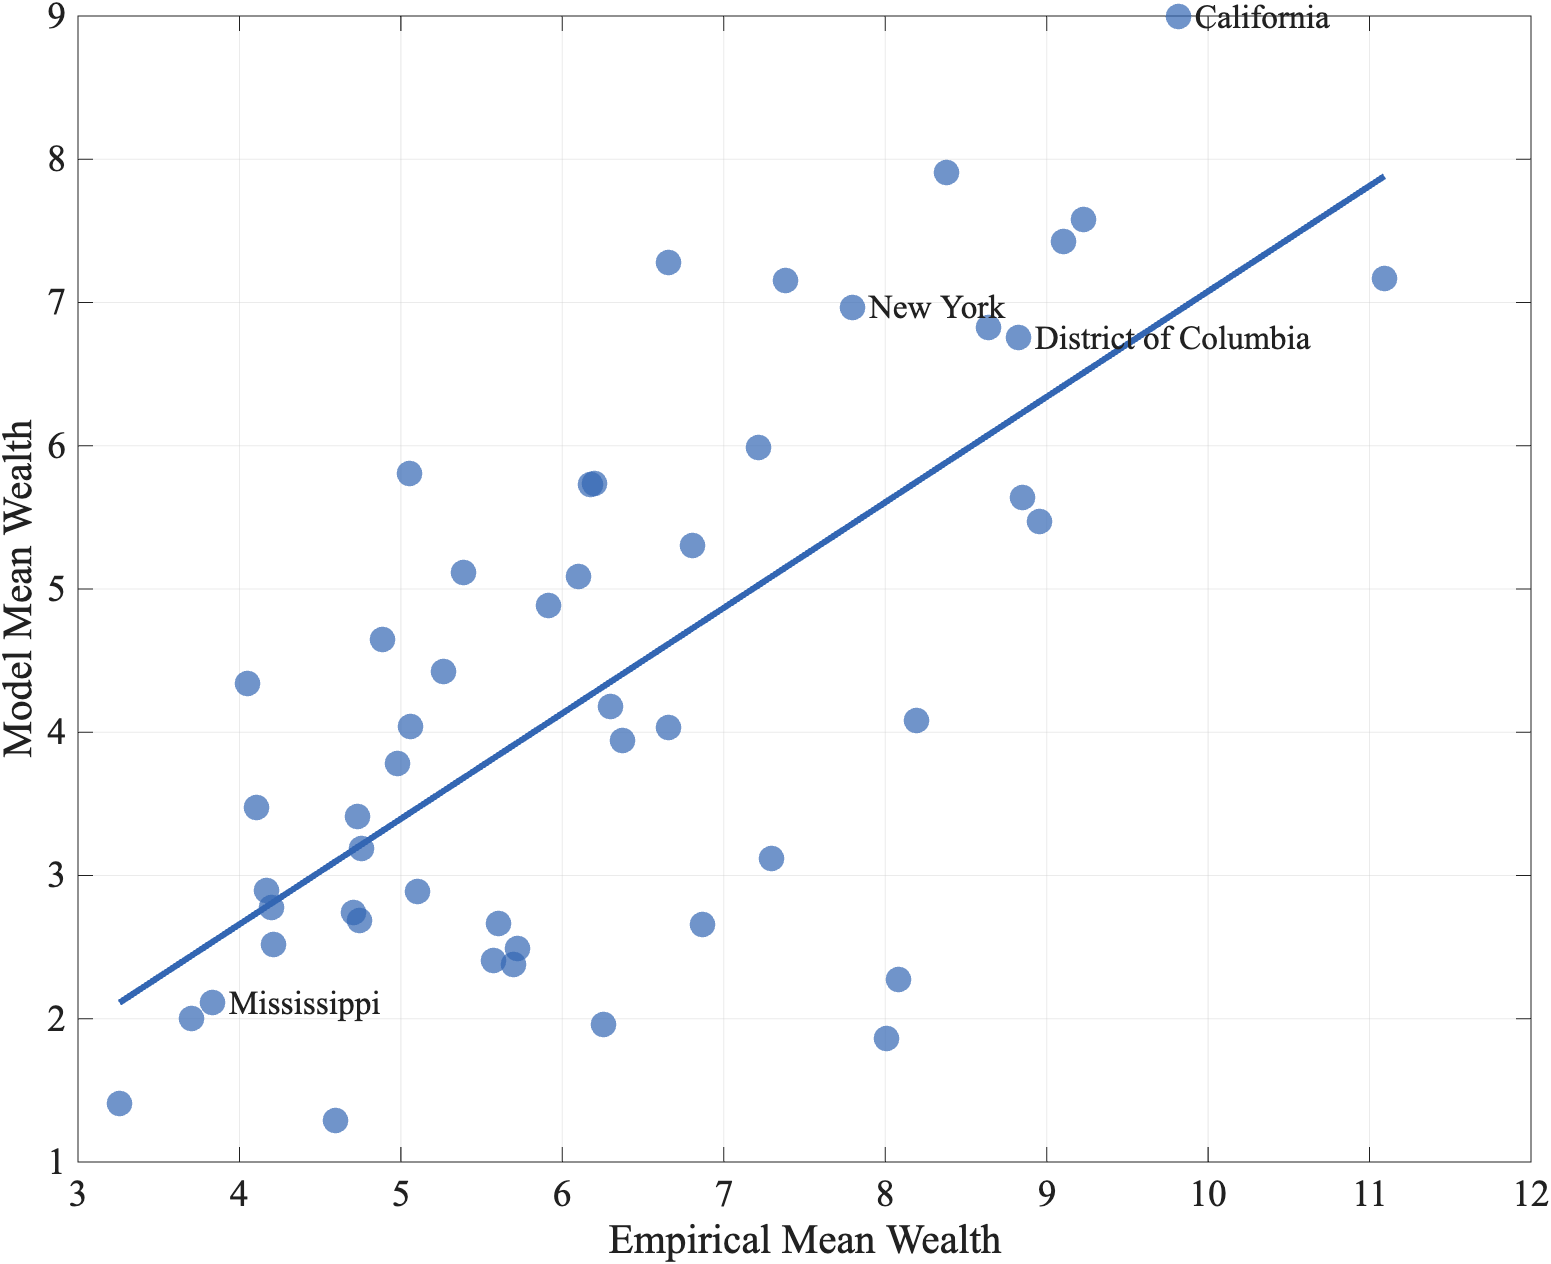
\includegraphics[width=\textwidth]{../Output/graph_comparison/out_sample_fit/out_sample_fit_model_mean_wealth.png}
        \caption{Wealth Comparisons}
        \label{fig:out_sample_wealth}
    \end{subfigure}
    \hfill
    \begin{subfigure}[b]{0.49\textwidth}
        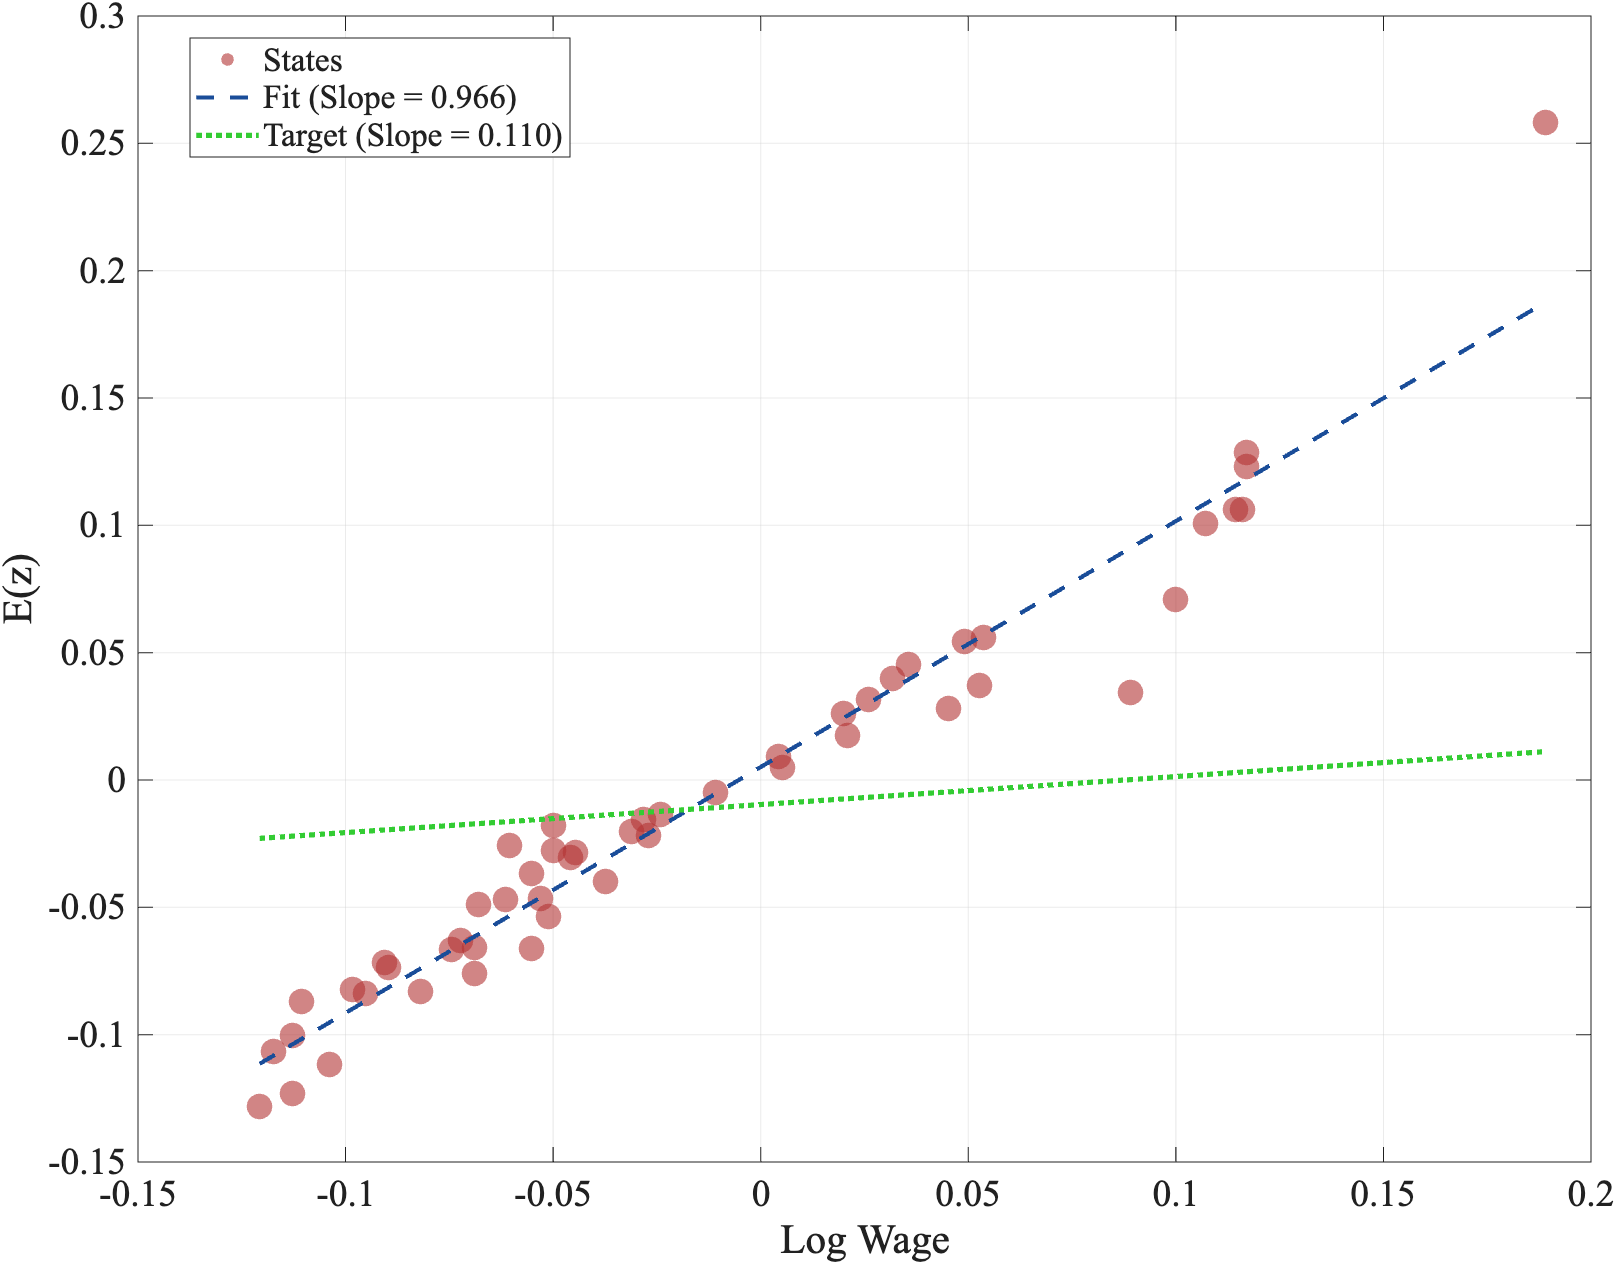
\includegraphics[width=\textwidth]{../Output/graph_comparison/out_sample_fit/out_sample_fit_e_z.png}
        \caption{Migration Sorting}
        \label{fig:out_sample_sorting}
    \end{subfigure}
    
    \vspace{1em}
    \begin{subfigure}[b]{0.49\textwidth}
        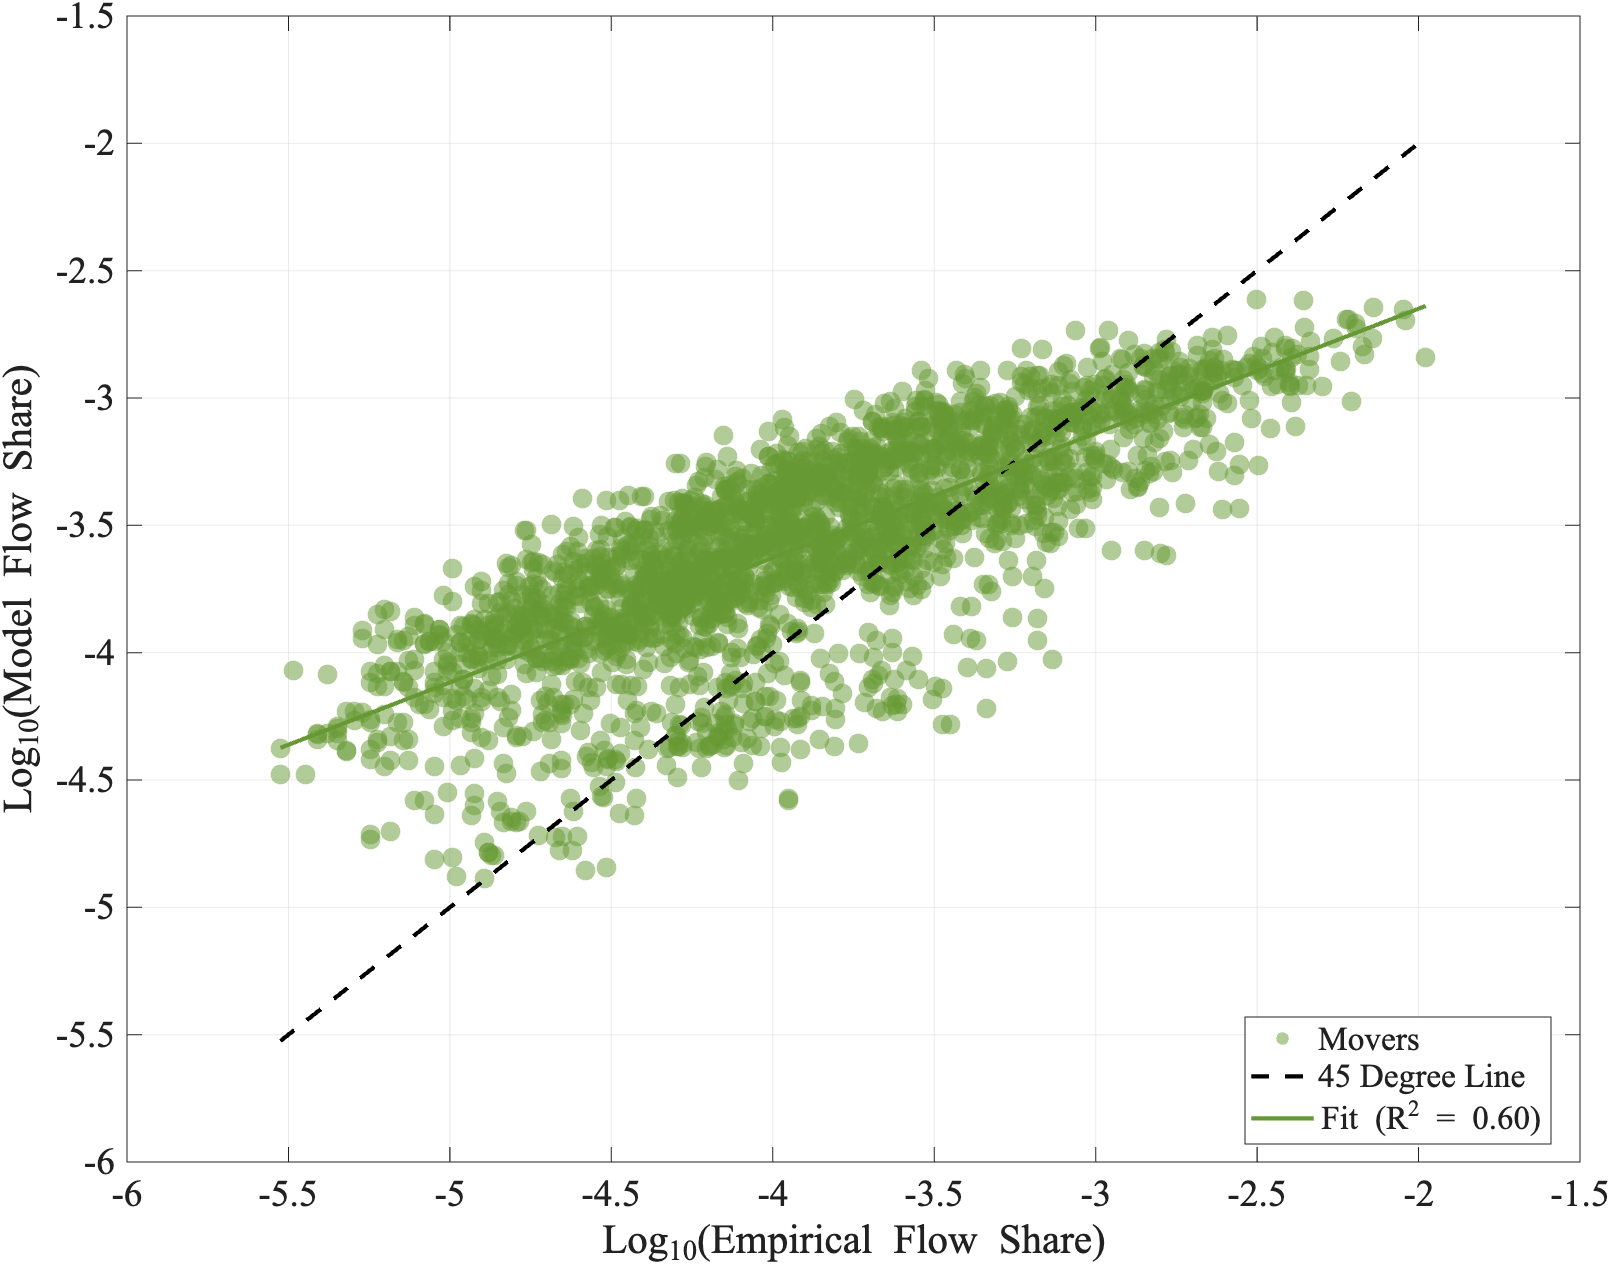
\includegraphics[width=\textwidth]{../Output/graph_comparison/out_sample_fit/out_sample_fit_log_10_model_flow_share.png}
        \caption{Bilateral Migration Flows}
        \label{fig:out_sample_flows}
    \end{subfigure}
    
    \begin{minipage}{\textwidth} \vspace{0.5em}
      \footnotesize{\textbf{Note:} Out-of-sample fit of the model along three dimensions: (a) average state-level wealth, (b) spatial sorting of productive workers across states, and (c) bilateral migration flows (in log shares) between states. In panel (a), the black line displays the OLS regression of model-implied mean wealth on empirical values from Geowealth-US 2010. In panel (b), the regression of expected productivity $E(z)$ on log wages (blue dashed line) tracks the slope of $0.11$ (green dotted line) from \cite{dvorkin_geography_2025}. In panel (c), the OLS regression of model-implied bilateral log migration shares on empirical values from the ACS 2010-2019 is shown.}
    \end{minipage}
\end{figure}


\subsection{Climate Change Damages}
The exogenous climate shock paths are derived from the county-level damage estimates of \citet{hsiang_estimating_2017}, who project economic impacts across six sectors under RCP~8.5 for the period 2080--2099. Their county-level data are aggregated to the state level using population and income weights, then mapped into the three channels of the Dvorkin \& Greaney framework:
\begin{table}[!htb]
\centering
\small
\renewcommand{\arraystretch}{1.2}
\begin{tabular}{lll}
\toprule
\textbf{Hsiang sector} & \textbf{Model channel} & \textbf{Aggregation weight} \\
\midrule
Labour (avg.\ low- \& high-risk) & Wage $(\Delta w)$ & Income-weighted \\
Agriculture (4 major crops) & Wage $(\Delta w)$, scaled by $s_\ell^{\text{agri}}$ & Income-weighted \\
Coastal damages & Wage $(\Delta w)$ & Income-weighted \\
\addlinespace
Mortality (deaths / 100k) & Amenity $(\Delta A)$, via VSL & Population-weighted \\
\addlinespace 
Violent and Property crime (crime / 100k) & Amenity $(\Delta A)$, via VSC & Population-weighted \\
Energy expenditures & Housing cost $(\Delta q)$ & Income-weighted \\
\bottomrule
\end{tabular}
\caption{Mapping of the six Hsiang et al.\ (2017) damage sectors into the three model shock channels.}
\label{tab:sector_mapping}
\end{table}
\paragraph{Sector-to-channel mapping}
A challenge in this framework is the translation of non-pecuniary empirical damages (mortality and crime) into the model's parameters. Because baseline amenities ($A_{\ell, \text{init}}$) are residuals centred around zero (as they explain location choice that is not captured by wage), evaluating amenity damages as a percentage of this baseline is somewhat spurious. Instead absolute amenity shocks ($\text{shock\_amenity}_\ell$) can be interpreted as consumption-equivalent welfare losses via the marginal rate of substitution ($MRS_{A,c} = 1/\gamma$). By scaling the monetary costs of mortality and crime by the national average income ($\bar{Y}_{\text{US}}$) and mapping them through $\gamma$, I convert empirical monetary damages into util shocks.

The three composite shocks are thus constructed as follows:
\begin{align}
  \text{shock\_wage}_\ell &= \frac{\bar L_\ell}{100}
    + \frac{\bar Y_\ell^{\text{agri}}}{100} \cdot s_\ell^{\text{agri}}
    - \frac{\bar C_\ell}{100}, \label{eq:shock_wage} \\
  \text{shock\_amenity}_\ell &= \gamma \left[ \left(\frac{\bar M_\ell}{100{,}000}\right) \frac{\text{VSL}}{\bar{Y}_{\text{US}}} + \left(\frac{\bar R_\ell}{100{,}000}\right) \frac{\mathbb{E}[\text{VSC}]}{\bar{Y}_{\text{US}}} \right], \label{eq:shock_amenity} \\
  \text{shock\_housing}_\ell &= \frac{\bar E_\ell}{100} \cdot s_\ell^{\text{energy}}, \label{eq:shock_housing}
\end{align}
where $\bar L_\ell$ is the income-weighted average labour productivity loss (\%), $\bar Y_\ell^{\text{agri}}$ the income-weighted agricultural yield change (\%), $s_\ell^{\text{agri}}$ the agriculture GDP share of state $\ell$ (BEA 2010--2015 average), $\bar C_\ell$ the income-weighted coastal damage (\% of county income), $\bar M_\ell$ the population-weighted additional mortality (deaths per 100k), $\bar R_\ell$ the population-weighted additional crime (crimes per 100k), $\bar E_\ell$ the income-weighted change in energy expenditures (\%), and $s_\ell^{\text{energy}}$ the state-level electricity expenditure share of personal income. For the amenity parameters, $\gamma$ is the CARA absolute risk aversion coefficient, $\text{VSL} = \$9.0\text{M}$ (2012 USD), and the expected unit cost of crime $\mathbb{E}[\text{VSC}]$ evaluates separately violent (\$205,782) and property (\$4,799) crimes following \citet{mccollister_cost_2010} and pooled with FBI UCR incident data. $\bar{Y}_{\text{US}} = \$48,668.71$ (2012 USD) is the national average income using the CPS-ORG data with the 2010--2015 average and the same restrictions as \citet{dvorkin_geography_2025}.\footnote{It means that one model unit equals roughly $\$48,668.71$.} These shocks enter the terminal steady state as:
\begin{align}
  w_{\ell, \text{term}} &= w_{\ell, \text{init}} \cdot (1 + \text{shock\_wage}_\ell), \label{eq:w_terminal}\\
  A_{\ell, \text{term}} &= A_{\ell, \text{init}} - \text{shock\_amenity}_\ell, \label{eq:A_terminal}\\
  q_{\ell, \text{term}} &= q_{\ell, \text{init}} \cdot (1 + \text{shock\_housing}_\ell). \label{eq:q_terminal}
\end{align}

\paragraph{Magnitudes}
The resulting state-level shocks are moderate in absolute terms (Table~\ref{tab:shock_magnitudes}), reflecting the fact that most of Hsiang et al.'s headline damage ($\approx$6\% of GDP) is diluted across different sectors and channels. The wage channel experiences an average decline of 1.0\%, following a North--South gradient driven by labour productivity losses, with Nebraska standing out as an outlier ($-4.2$ \%) due to its agricultural exposure. The housing cost channel remains very small and spatially diffuse (averaging just $+0.2$ \%). Regarding non-pecuniary damages, under the baseline calibration of $\gamma = 3$, the drop in local amenities averages 1.01\% in consumption-equivalent terms. However, this national average hides spatial heterogeneity: the amenity degradation peaks at 7.81\% in the hardest-hit states, such as Florida, while colder states like Maine and Alaska experience a consumption-equivalent amenity gain of up to 3.50\% due to a reduction in winter mortality.
\begin{table}[!htb]
\centering
\small
\begin{tabular}{lrrrr}
\toprule
\textbf{Shock} & \textbf{Min} & \textbf{Max} & \textbf{Mean} & \textbf{Median} \\
\midrule
$\text{shock\_wage}$    & $-4.2\%$ (NE) & $+0.6\%$ (ND) & $-1.0\%$ & $-0.9\%$ \\
$\text{shock\_amenity}$ & $-3.5\%$ (ME) & $+7.8\%$ (FL) & $+1.0\%$ & $+0.6\%$ \\
$\text{shock\_housing}$ & $-0.0\%$ (WA) & $+0.4\%$ (AR) & $+0.2\%$ & $+0.2\%$ \\
\bottomrule
\end{tabular}
\caption{Summary statistics of the three composite climate shocks across 51 states (DC included). Signs: negative wage $=$ loss; positive amenity $=$ welfare deterioration (higher mortality); positive housing $=$ higher housing cost. Note that $\text{shock\_amenity}$ is reported in consumption-equivalent percentage terms (the absolute util shock divided by the CARA parameter $\gamma = 3$).}
\label{tab:shock_magnitudes}
\end{table}
Figure~\ref{fig:damage_maps} displays the spatial distribution of all three shocks. The wage channel shows a clear North--South gradient, driven primarily by the labour productivity loss, with Nebraska as an outlier due to its very large agricultural exposure. The amenity channel is dominated by heat-related mortality concentrated in the Gulf states and Florida. The housing cost channel is small and spatially diffuse.
\begin{figure}[htb]
  \centering
  \caption{Spatial Distribution of Climate Damages}
  \label{fig:damage_maps}
  \begin{minipage}[t]{0.32\textwidth}
    \centering
    \small{A. Wage Damages ($\Delta w$)}
    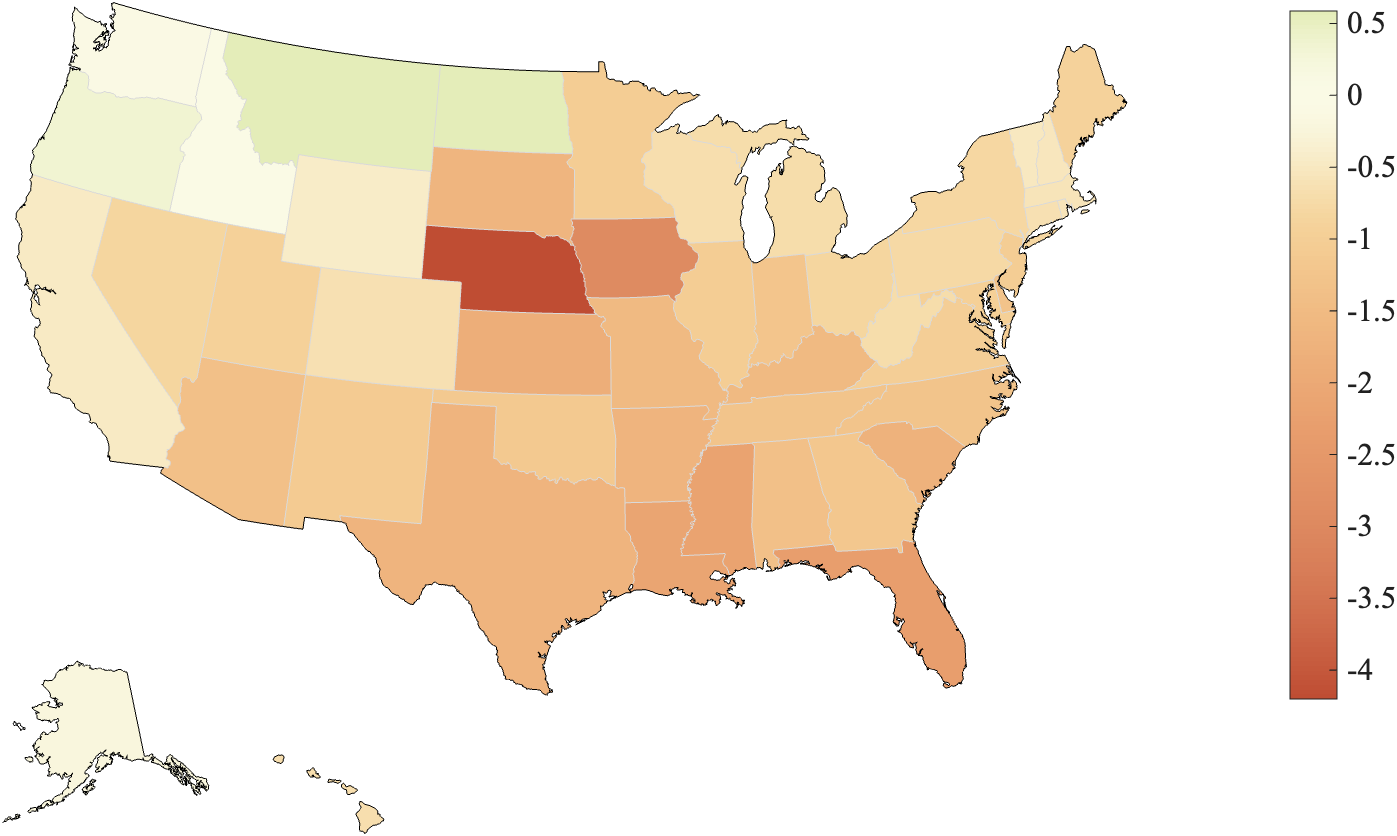
\includegraphics[width=\textwidth]{../Output/big_nu/graph_perfect_foresight/damage_maps/damage_maps_damage_wage.png}
  \end{minipage}\hfill
  \begin{minipage}[t]{0.32\textwidth}
    \centering
    \small{B. Amenity Damages ($\Delta A$)}
    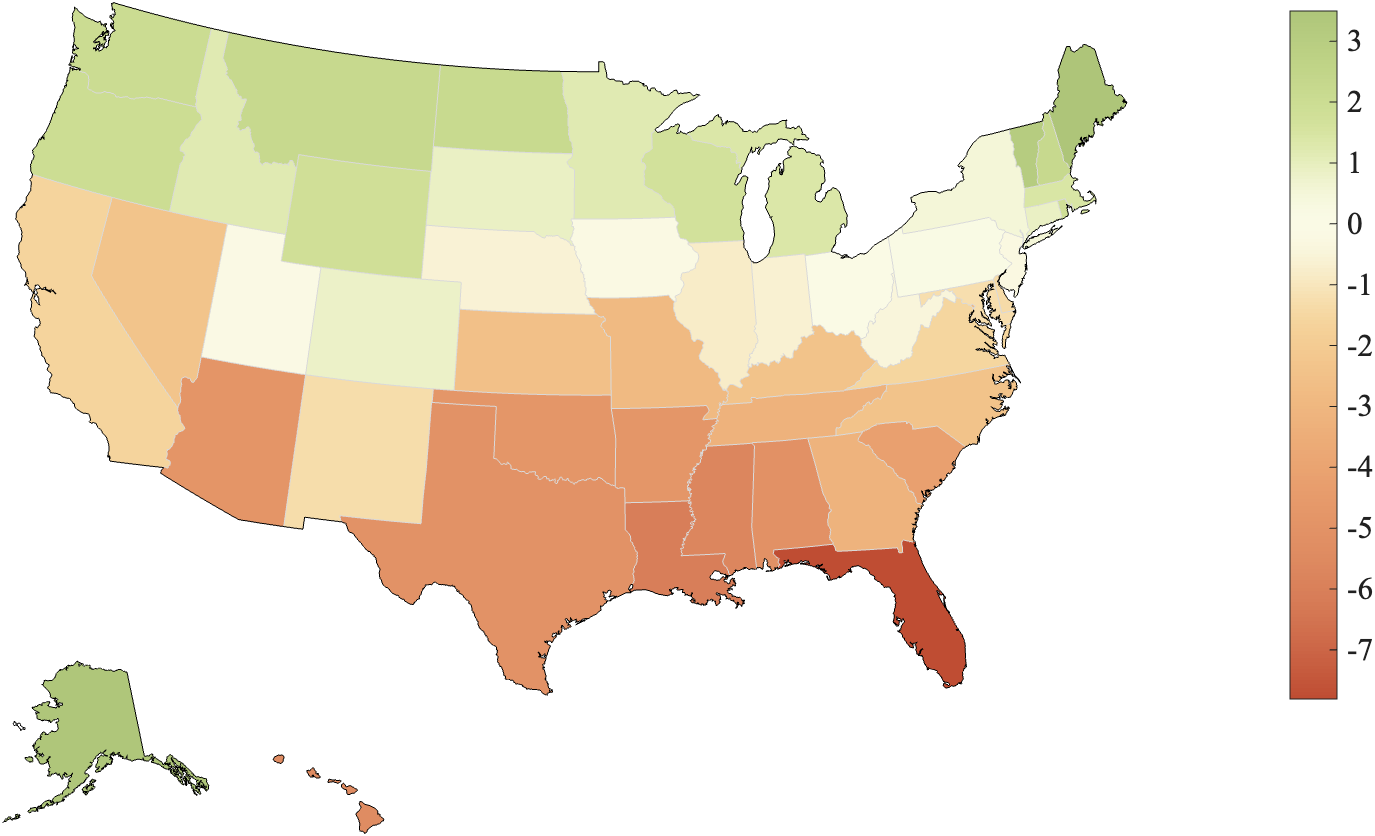
\includegraphics[width=\textwidth]{../Output/big_nu/graph_perfect_foresight/damage_maps/damage_maps_damage_amenity.png}
  \end{minipage}\hfill
  \begin{minipage}[t]{0.32\textwidth}
    \centering
    \small{C. Housing Damages ($\Delta q$)}
    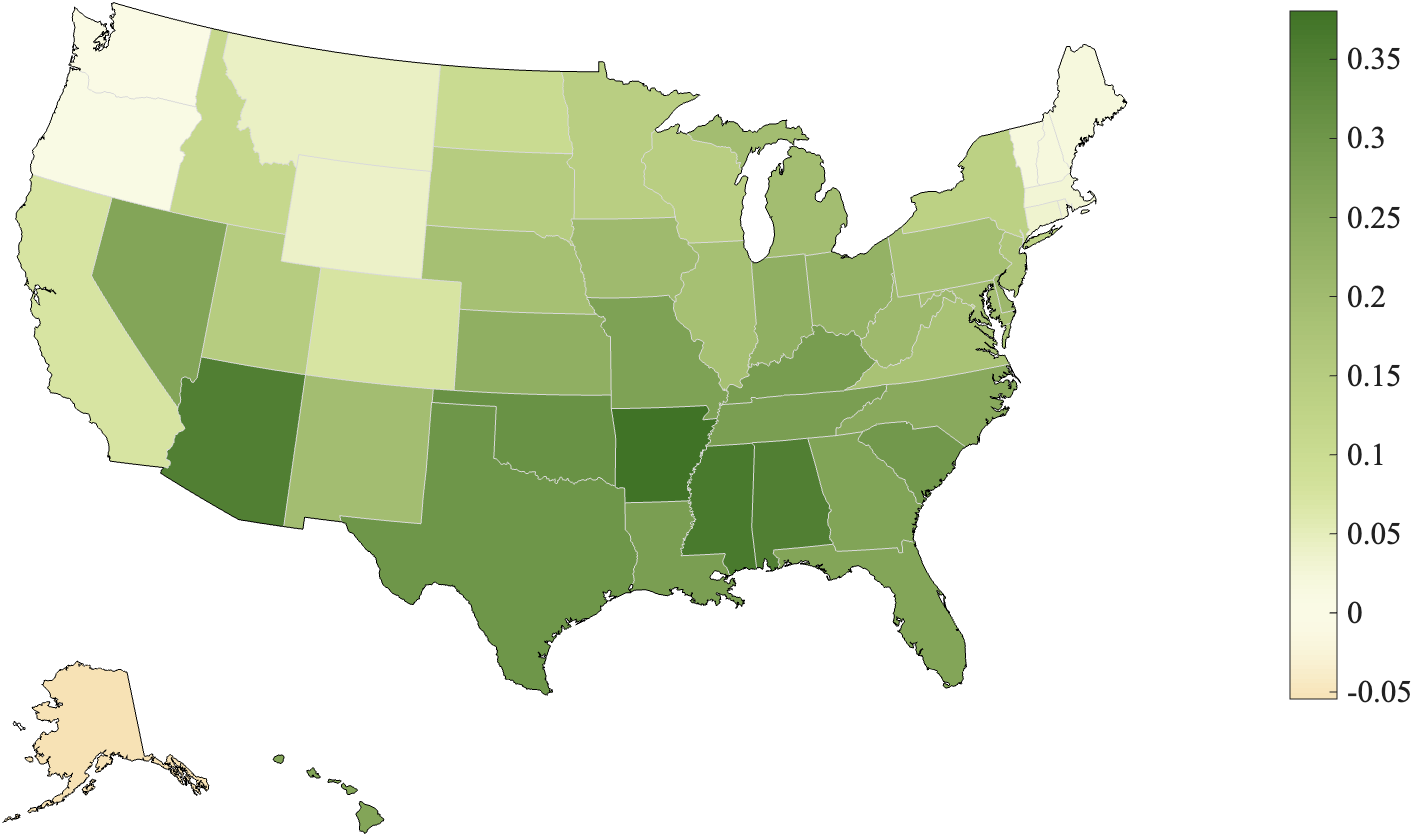
\includegraphics[width=\textwidth]{../Output/big_nu/graph_perfect_foresight/damage_maps/damage_maps_damage_housing.png}
  \end{minipage}
  \begin{minipage}{\textwidth}
  \vspace{0.5em}
  \footnotesize{\textbf{Note:} State-level spatial distribution of calibrated RCP 8.5 climate damage shocks across $J=51$ states. Panel~(a): percentage wage damage $\Delta w_\ell = \text{shock\_wage}_\ell \times 100$, where $w_{\ell, \text{term}} = w_{\ell, \text{init}}(1 + \text{shock\_wage}_\ell)$ combines labour productivity, agricultural yield, and coastal loss channels. Panel~(b): amenity loss expressed in consumption-equivalent percentage points, $\Delta A_\ell^{\text{CE}} = (\text{shock\_amenity}_\ell / \gamma) \times 100$, where $A_{\ell, \text{term}} = A_{\ell, \text{init}} - \text{shock\_amenity}_\ell$ based on temperature mortality and monetised crime rates. Panel~(c): percentage housing cost shock $\Delta q_\ell = \text{shock\_housing}_\ell \times 100$, where $q_{\ell, \text{term}} = q_{\ell, \text{init}}(1 + \text{shock\_housing}_\ell)$ through energy demand.} \end{minipage}
\end{figure}

\section{Quantitative Results}
This section provides an overview of the various scenarios and counterfactuals conducted. The dynamic simulation computes the economy's transition over a horizon of $T_{\text{sim}} = 500$ years, which includes a 90-year linear climate damage ramp followed by 410 periods of steady-state padding to ensure terminal convergence. The main scenario serves as the baseline, wherein agents possess perfect foresight regarding climate change, anticipating future shifts in wages and amenities. I introduce a scenario that varies agents' expectation. In the Myopia scenario agents are unaware of future trajectories and base their decisions on current conditions. Then, the No Migration scenario is a counterfactual setting where migration costs are assumed to be infinite ($\psi_{j\ell} = 10^8$ for $j \neq \ell$), shutting down migration; in the No Saving scenario agents are not allowed to save. Additional scenarios can be found in the Appendix~\ref{app:additional}.
\subsection{Baseline Dynamic Transition (Perfect Foresight)}
Figure~\ref{fig:trans_dyn_pf} illustrates that the aggregate effects of climate change on earnings and wealth are modest, yet they conceal substantial regional disparities, as depicted in Figure~\ref{fig:trans_map_pf}.
\paragraph{National aggregate and transition dynamics}
The transition dynamics reveal the permanent income and amenity effect depicted in Equation~\ref{eq:saving_climate} during the 2010--2100 period. Aggregate wealth increases by 4.5\% at its peak, as agents anticipate future climate damages and accumulate savings before consuming this wealth to smooth the effect of climate change over time. The aggregate wealth and wealth-to-income ratios slowly transition towards new steady-state values over approximately 300 years that remain very close to their baseline levels, which shows that an analysis limited to national aggregates would miss substantial spatial heterogeneity. The interstate migration rate\footnote{Calculated as the national population share changing state of residence between two periods: $m_t = \sum_{\ell,z} \Lambda_t(\ell,z) [1 - \mu_{\ell \ell,t}(z)] / \sum_\ell L_{\ell,t}$} experiences a slight increase in response to climate change before returning to its baseline value in the new steady state. But an aggregate migration rate masks important shifts in the nature of mobility and the migration patterns. In fact, even if the overall rate of migration remains modest, the long-run composition and population size within individual states go through massive changes. Similarly, the aggregate average wage appears almost unaffected by climate change. At the national scale, there is only a marginal increase in the average wage (equivalent to an increase of roughly 250 USD per year for a baseline unit wage of 50,000 USD). This small aggregate effect is driven by population reallocation: because the national average wage is weighted by state population shares, the reallocation of workers towards high-wage states, which are located for the major part in the North of the US so relatively less impacted by climate change, offsets localised wage declines.

In short, the national aggregate dynamics are useful to look at the speed of adjustment and the anticipation of future damages. First, due to migration frictions, the adaptation process is slow; it takes roughly 300 years for the economy to reach the new steady state, despite the fundamental climate shocks stabilising 200 periods earlier. Second, these dynamics exhibit agents' anticipation of future damages, as they begin saving well before the most severe damages are realised to smooth the coming drop in wage and amenity. Nevertheless, national aggregates mask large spatial heterogeneity, are driven by the reallocation of populations across states and thus miss a part of the story.
\begin{figure}[!htb]
  \centering
  \caption{Dynamic Moments (Perfect Foresight)}
  \label{fig:trans_dyn_pf}
  \begin{minipage}[t]{0.4\textwidth}
    \centering
    \small{(a) Earnings}
    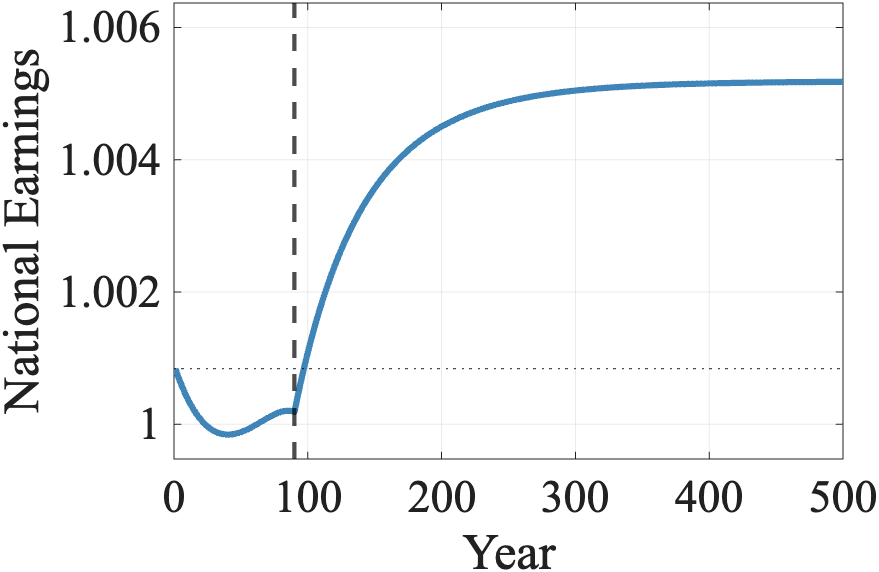
\includegraphics[width=\textwidth]{../Output/big_nu/graph_perfect_foresight/dynamic_moments/dynamic_moments_national_earnings.png}
  \end{minipage}\hfill
  \begin{minipage}[t]{0.4\textwidth}
    \centering
    \small{(b) Mobility}
    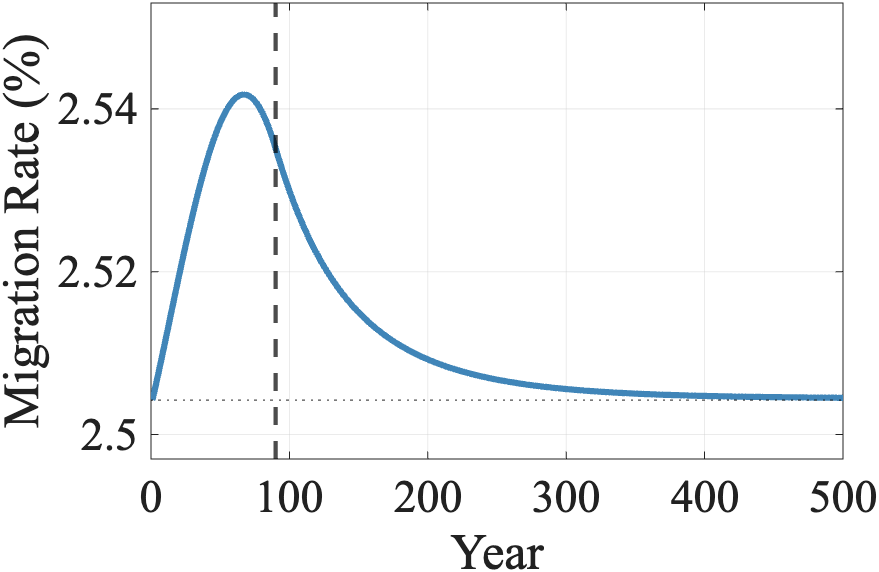
\includegraphics[width=\textwidth]{../Output/big_nu/graph_perfect_foresight/dynamic_moments/dynamic_moments_national_mobility.png}
  \end{minipage} \\[2ex]
  \begin{minipage}[t]{0.4\textwidth}
    \centering
    \small{(c) Wealth}
    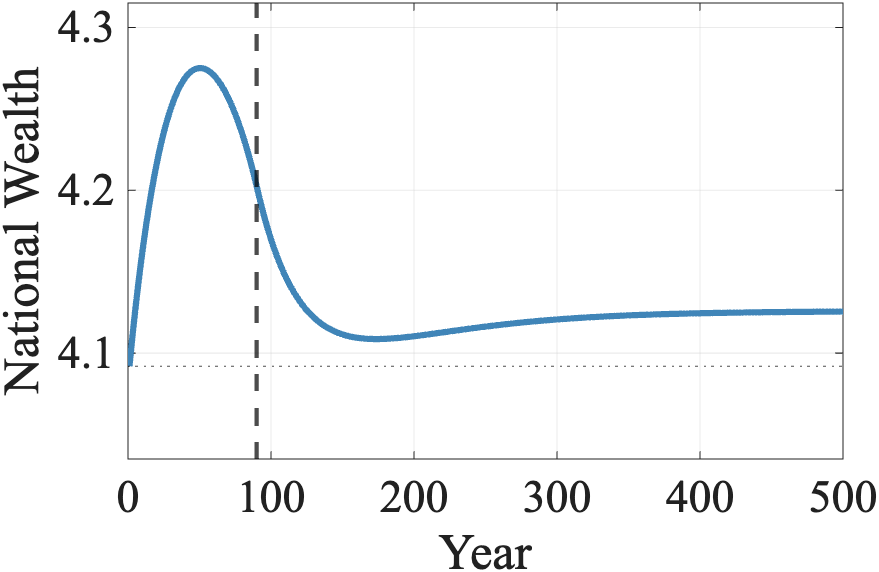
\includegraphics[width=\textwidth]{../Output/big_nu/graph_perfect_foresight/dynamic_moments/dynamic_moments_national_wealth.png}
  \end{minipage}\hfill
  \begin{minipage}[t]{0.4\textwidth}
    \centering
    \small{(d) W/Y Ratio}
    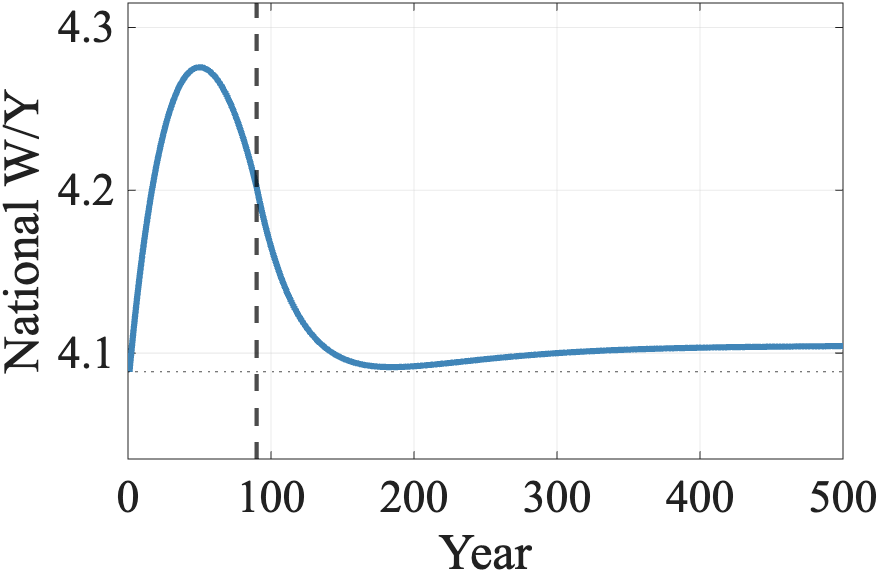
\includegraphics[width=\textwidth]{../Output/big_nu/graph_perfect_foresight/dynamic_moments/dynamic_moments_national_wy.png}
  \end{minipage} \begin{minipage}{\textwidth} 
  \vspace{0.5em}
  \footnotesize{\textbf{Note:} Aggregate macroeconomic time series under Perfect Foresight, 2010--2500+. Panel (a): national total disposable labour earnings $Y_t = \sum_{\ell=1}^J \tilde{w}_{\ell,t} (L_{\ell,t} + \sum_z z \Lambda_t(\ell,z))$. Panel (b): national gross annual inter-state migration rate $m_t = \sum_{\ell,z} \Lambda_t(\ell,z) [1 - \mu_{\ell \ell,t}(z)] / \sum_\ell L_{\ell,t}$. Panel (c): total national wealth holdings $W_t = \sum_{\ell,z} \bar{a}_t(\ell,z) \Lambda_t(\ell,z)$. Panel (d): aggregate wealth-to-earnings ratio $(W/Y)_t = W_t / Y_t$, capturing precautionary asset accumulation ahead of climate shocks and subsequent decumulation.} \end{minipage}
\end{figure}
\paragraph{Spatial differences across the two Steady States}
\begin{figure}[!htb]
  \centering
  \caption{Transition Maps (Perfect Foresight)}
  \label{fig:trans_map_pf}
  \begin{minipage}[t]{0.4\textwidth}
    \centering
    \small{(a) $\Delta$ Mean Welfare (CE)}
    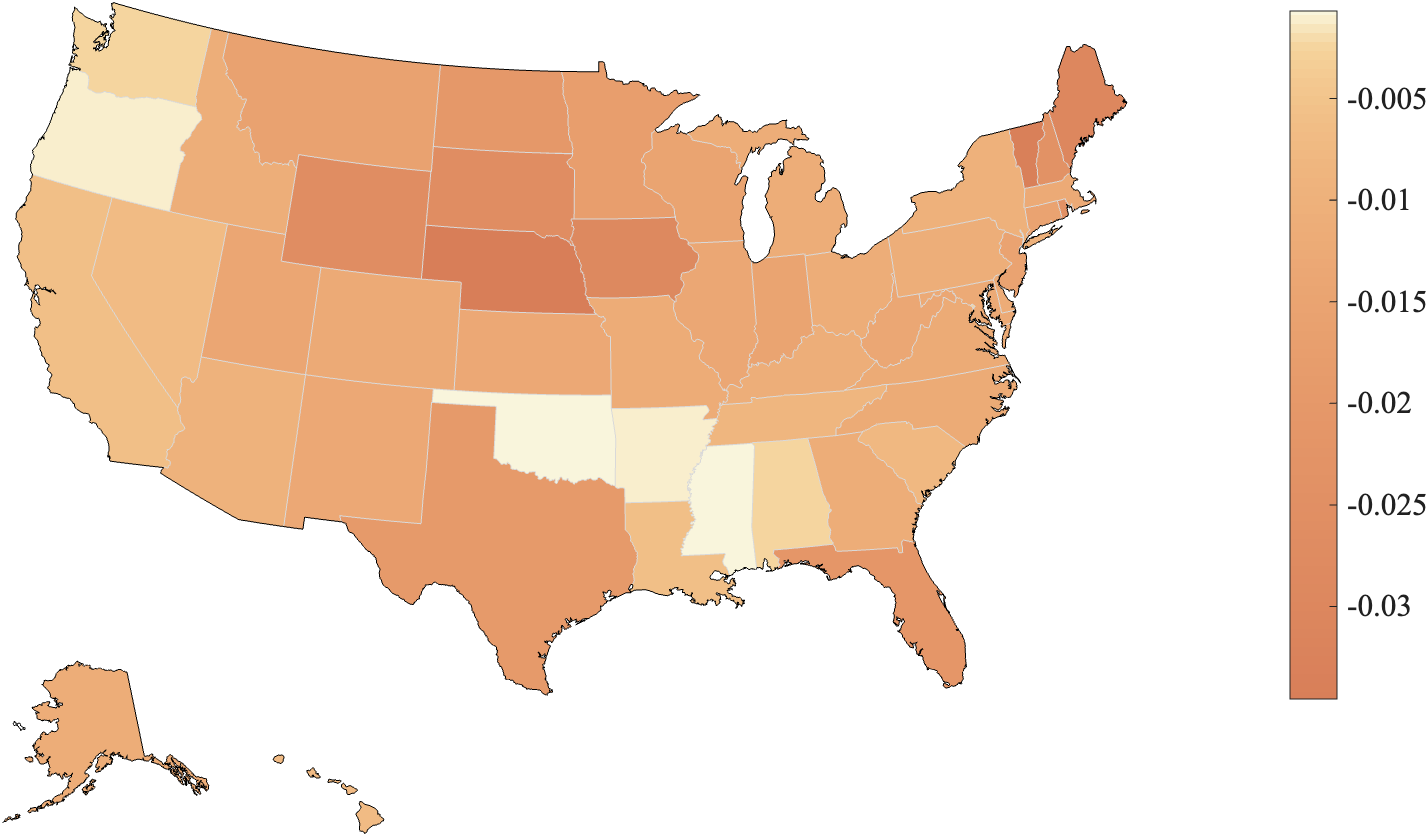
\includegraphics[width=\textwidth]{../Output/big_nu/graph_perfect_foresight/transition_maps/transition_maps_delta_mean_welfare_ce.png}
  \end{minipage}\hfill
  \begin{minipage}[t]{0.4\textwidth}
    \centering
    \small{(b) $\Delta$ W/Y Ratio in level}
    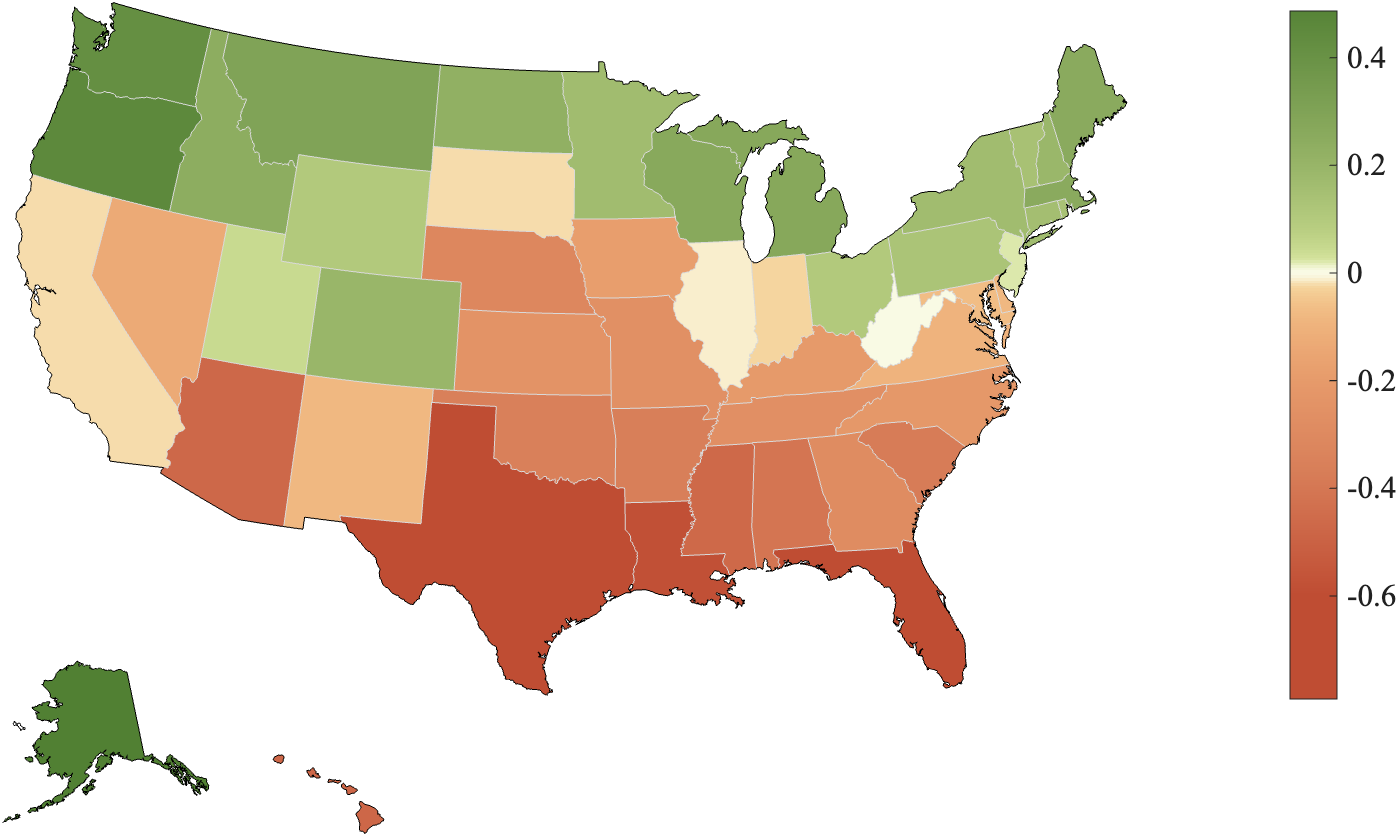
\includegraphics[width=\textwidth]{../Output/big_nu/graph_perfect_foresight/transition_maps/transition_maps_wealth_income_ratio_changes.png}
  \end{minipage}\\[2ex]
  \begin{minipage}[t]{0.4\textwidth}
    \centering
    \small{(c) $\Delta$ Local Population (\%)}
    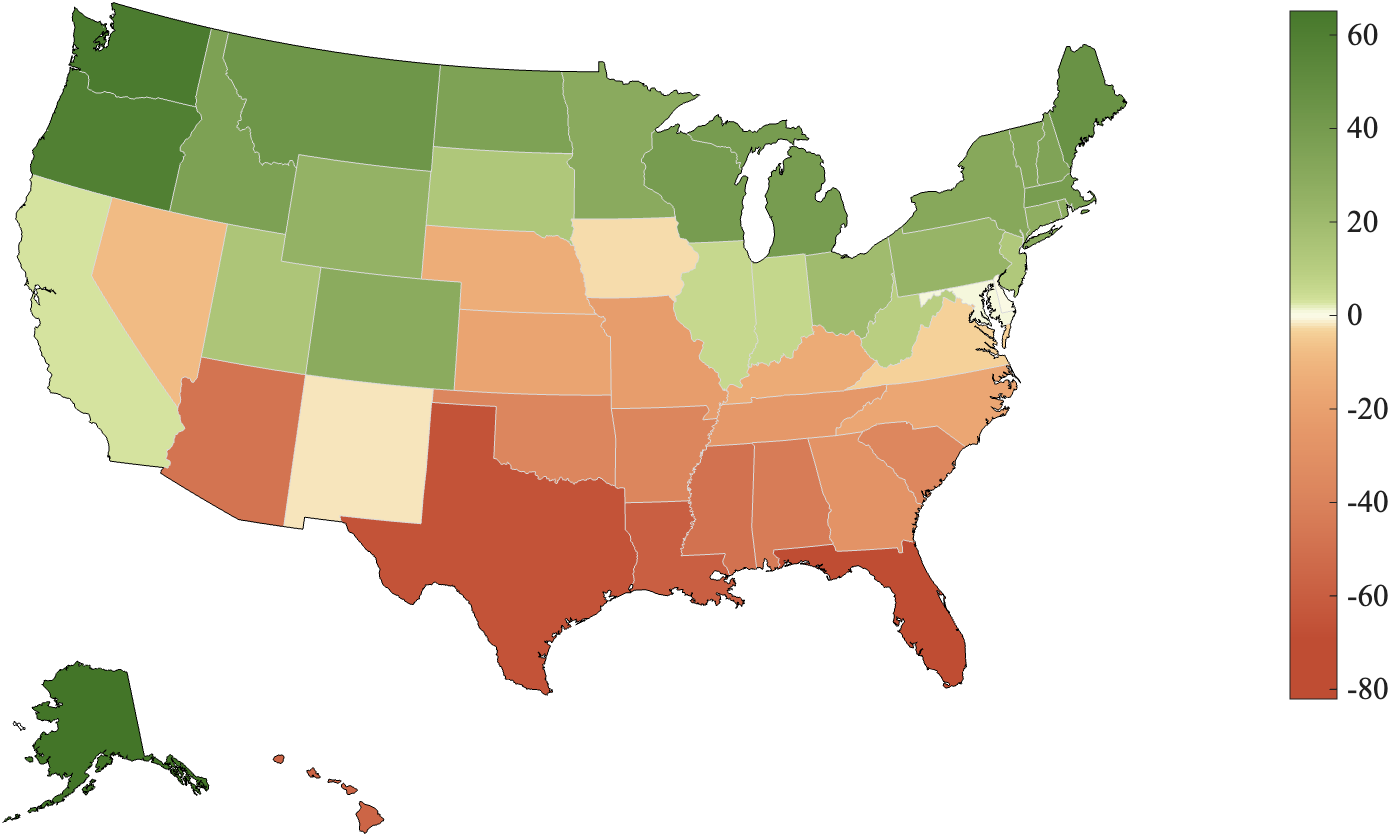
\includegraphics[width=\textwidth]{../Output/big_nu/graph_perfect_foresight/transition_maps/transition_maps_local_pop_changes_pct.png}
  \end{minipage}\hfill
  \begin{minipage}[t]{0.4\textwidth}
    \centering
    \small{(d) $\Delta$ Mean Wealth (\%)}
    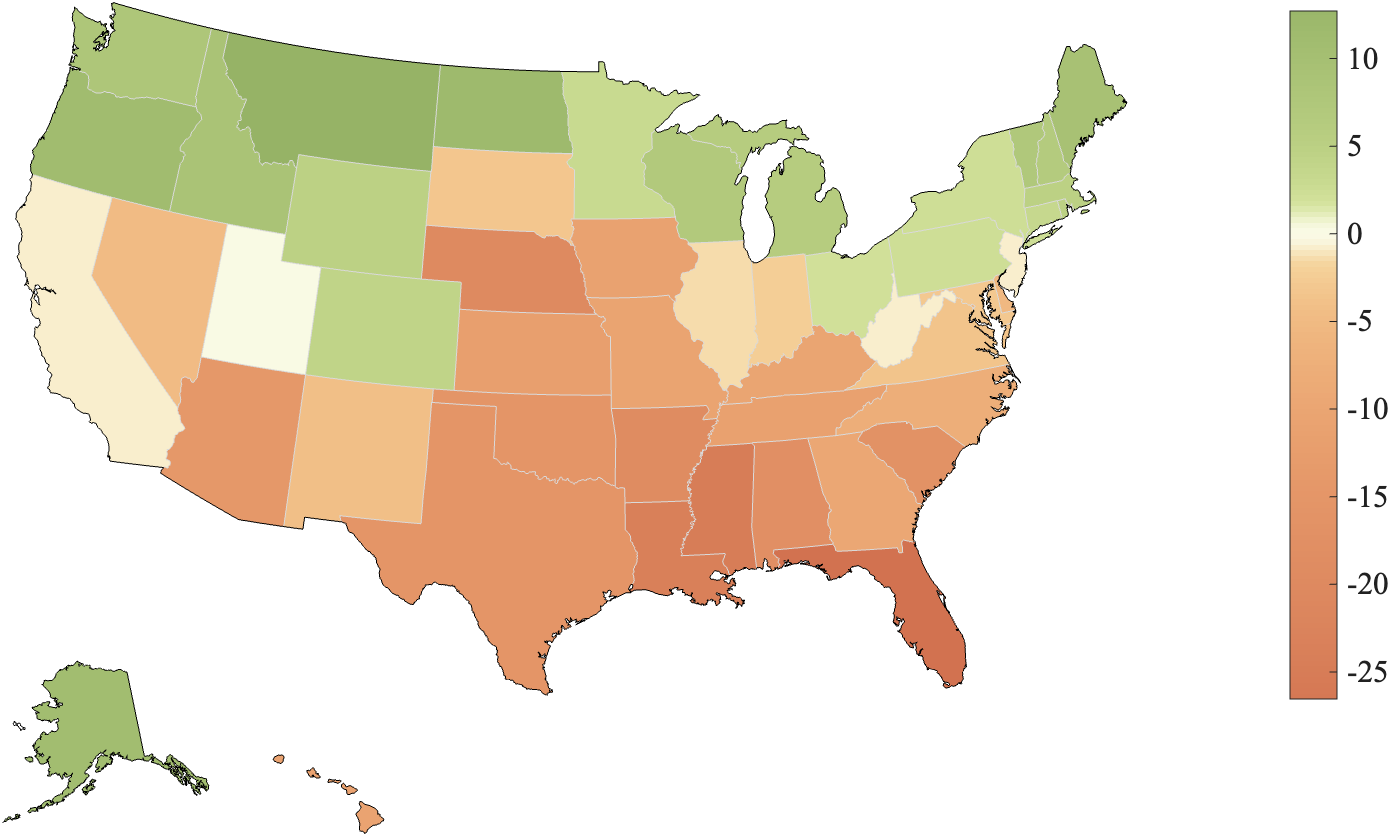
\includegraphics[width=\textwidth]{../Output/big_nu/graph_perfect_foresight/transition_maps/transition_maps_pop_changes_pp.png}
  \end{minipage}
   \begin{minipage}{\textwidth}
  \vspace{0.5em}
  \footnotesize{\textbf{Note:} Spatial maps comparing the terminal steady state under 2100 climate parameters ($SS_\text{term}$) to the initial 2010 baseline steady state ($SS_\text{init}$) under Perfect Foresight. Panel (a): change in mean Certainty Equivalent welfare $\Delta \text{CE}_\ell = \overline{\text{CE}}_{\ell, \text{term}} - \overline{\text{CE}}_{\ell, \text{init}}$, with $\overline{\text{CE}}_\ell = \frac{1}{L_\ell} \sum_z \Lambda(\ell,z) [\kappa \bar{a}_\ell(z) + \Xi_\ell(z)]$. Panel (b): change in state wealth-to-earnings ratio $\Delta (W/Y)_\ell = (W/Y)_{\ell, \text{term}} - (W/Y)_{\ell, \text{init}}$. Panel (c): relative population percentage change $\Delta L_\ell\% = 100 \times (L_{\ell, \text{term}} - L_{\ell, \text{init}})/L_{\ell, \text{init}}$. Panel (d): percentage change in state mean per-capita wealth $\Delta \bar{a}_\ell\%$.} \end{minipage}
\end{figure}
Comparing the initial and final steady states reveals the spatial heterogeneity that is hidden by national aggregates. The model predicts a strong North-South gradient in population reallocation: the South-East experiences an important drop in population, most notably a local population decline of 80\% in Florida and 20 to 30\% across the broader region, while the North-East and specific northern states like Alaska see local population go up by 20 to 30\% and up to 60 percent, respectively. 
This spatial gradient is similar when looking at the wealth accumulation and the wealth-to-income ratio. States such as Florida and Louisiana experience a drop in mean wealth of approximately 25 percent, contrasted with increases of over 10\% in states like Montana and Oregon. The spatial distribution of these effects is not symmetric: the magnitude of local economic drop in the more affected regions is larger than the expansions in the other states. National aggregates fail to capture this asymmetry due to the weighting effect: heavily damaged states like Florida lose over 70\% of their population so their contribution to the national aggregate wealth shrinks, masking the severity of wealth destruction. Furthermore, while the decline in local wages correlates with a decline in wealth, the proportional drop in wealth systematically exceeds the drop in wages, driving the wealth-to-income ratio down in tandem with per-state mean wealth. 

Despite the heterogeneous spatial impacts and reactions, the welfare implications, measured in consumption equivalent terms, are negative across all regions. No single state is strictly better off after climate change. In a dynamic spatial equilibrium with idiosyncratic preference shocks, workers evaluate welfare not only on local fundamentals, but on the option value of the entire spatial network. The degradation of amenities and wages in southern states reduces the expected continuation value of migration for all agents, regardless of their current location. A more detailed welfare analysis is provided in Section 4.3.

Wealth changes across the two steady states come from the mechanisms described in Equations \ref{eq:wealth_decomposition} and \ref{eq:intensive_margin_decomposition} of Section 2.3: damage-dampening, risk effect, spatial option value, spatial transition and compositional margin.
To disentangle these mechanisms, Figure \ref{fig:trans_wy_pf} utilises a wealth change decomposition that captures all the effects exhibited.\footnote{More details for the computation of the decomposition are given in Appendix~\ref{app:algorithms}.} The decomposition yields several insights. First, the risk effect is quantitatively negligible. While changes in the monetary magnitude of mean-reversion play a bigger role than the risk effect (since a drop in income reduces the need for saving against mean-reverting shocks), the vast majority of the heterogeneity in wealth dynamics is driven by the three spatial components. In particular, the spatial option effect, which captures shifts in migration probabilities and implicit changes in non-market amenities, is the primary driver of changes in wealth across steady states. As theorised in Section 2.3, workers in states like Alaska or Oregon accumulate additional precautionary wealth to insure against the risk of drawing an idiosyncratic shock that would make them migrate to a climate-damaged state. On the other side of the table, in severely impacted states like Florida or Louisiana, the spatial option effect suppresses wealth accumulation. Workers in these regions anticipate that conditional on drawing a sufficiently large preference shock to migrate, they will likely relocate to a state with superior wages or amenities, thus reducing their current precautionary savings motive.

Then, the spatial transition effect accounts for changes in wealth driven by shifts in the historical origins of a state's population that is governed by the interaction between moving cost and the geographic distribution of climate damages. When spatially correlated climate damages decrease the fundamental value of Southern states, the resulting wave of migration does not disperse uniformly across the country because moving costs penalise long-distance migration. Instead, it flows into nearby states. The average wealth in these adjacent states (that are for the most part also hit by climate change) is dragged down, as their incoming migration comes more often from damaged neighbouring states. For the most damaged states their in-migration rate decreases, trapping their wealth dynamics to the localised economic depression. For relatively undamaged states, the spatial transition effect is often positive. Because their fundamental value rises relative to the rest of the country $\mu_{jj}$ increases for those states. By having a larger share of their  residents and proportionally fewer immigrants, the historical origin of these safe states shifts towards higher average wealth. This mechanism is sensitive to a state's baseline wealth relative to its immigrant origin. For instance, severely damaged states with historically low baseline wealth (such as Louisiana) can exhibit a positive spatial transition effect: their population flees and the remaining population comes from states that are historically wealthier. The attractive states that are relatively close to the damaged states (such as Montana) can exhibit a negative transition effect if they experience an influx of immigrants whose origin-state wealth is lower than the haven's baseline.

Finally, the compositional sorting effect isolates the change in wealth attributable to the endogenous spatial sorting of productivity types. Severely impacted states like Florida and Louisiana lose high-productivity workers who save more than the other workers (mainly because they are more prone to mean-reverting saving), which reduces the mean productivity and mean wealth in those states. States like Alaska and Oregon experience the reverse, absorbing high-productivity workers and thereby increasing their mean wealth. It should be noted, however, that this compositional effect is not strictly monotonic across the climate-impact gradient; several lightly affected states also exhibit negative compositional sorting. Ultimately, while productivity sorting operates in the expected theoretical direction, it remains a secondary driver of the overall spatial variation in wealth changes.
\begin{figure}[!htb]
  \centering
    \caption{Wealth's Change Decomposition (Perfect Foresight)}
  \label{fig:trans_wy_pf}
  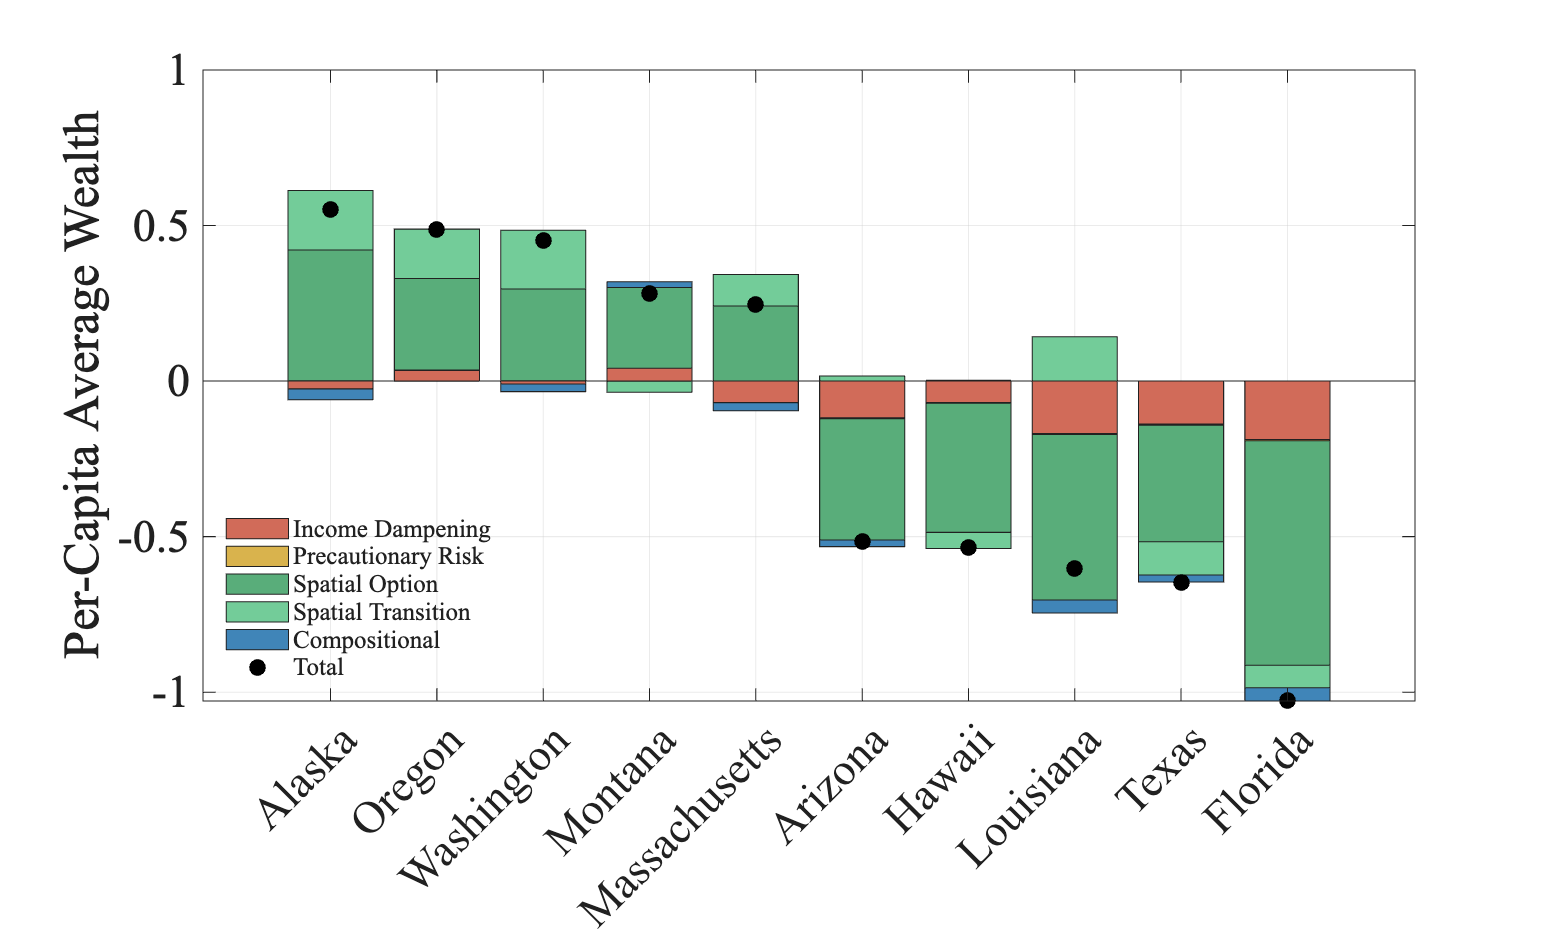
\includegraphics[width=\textwidth]{../Output/big_nu/graph_perfect_foresight/exact_percapita_decomposition_bar_no_counterfactual_no_counterfactual.png}
  \begin{minipage}{\textwidth}
  \vspace{0.5em}
  \footnotesize{\textbf{Note:} Structural shift-share decomposition of the state-level per-capita wealth change $\Delta \bar{a}_\ell = \bar{a}_{\ell, \text{term}} - \bar{a}_{\ell, \text{init}}$ under Perfect Foresight into five margins: (1) Income Dampening: savings adjustments to income changes evaluated at the baseline autarky network; (2) Precautionary Risk: shifts in savings due to altered income variance evaluated at autarky; (3) Spatial option: network premium from accumulating wealth over the baseline spatial network versus autarky; (4) Spatial Transition: change in the migration network evaluated at the new savings behaviour; (5) Compositional: changes in local productivity shares.}
  \end{minipage}
\end{figure}
\paragraph{Inequality Indices: Intra- and Inter-State Dynamics}
The divergence of wealth between the North and the South alters the distribution of wealth across the country. To quantify this, I decompose the variance of wealth and welfare into intra-state dynamics (the variance of wealth within each state) and inter-state dynamics (the variance of mean wealth across states). These variances are population-weighted to reflect the actual distribution of workers. Note that because the population distribution becomes increasingly concentrated as climate migration empties the South, the inter-state variance is mostly driven by the largest states, which tends to dampen the measured magnitude of spatial inequality.

Figure~\ref{fig:ineq_pf} presents the evolution of these inequality metrics. For wealth, intra-state variance decreases in almost all states, with the exception of climate havens like Oregon and Washington. This within-state compression is driven by two forces. First, the damage-dampening effect compresses the precautionary saving gap between high- and low-productivity workers. Second, the compositional sorting mechanism drives high-productivity (and thus wealthier) workers out of damaged states, leaving behind a poorer, more homogeneous population. Oregon and Washington experience rising internal inequality because they absorb a diverse influx of migrants across the wealth spectrum, mixing with their native populations. At the national level, the inter-state wealth variance exhibits a non-monotonic transition. It starts by decreasing slightly as everyone engages in transitional saving to smooth the permanent income and amenity drop, boosting Southern wealth in the short run. In the long run, inter-state wealth variance increases by 6 percent, reflecting the permanent spatial divergence between the wealth-depleted South and the wealth-accumulating North.

In contrast to wealth, the inter-state variance in welfare strictly decreases, dropping by up to 8\% by 2100 before stabilising at a permanent 5\% decline. This divergence between wealth and welfare inequality comes from the option value of migration. While climate change concentrates physical wealth in the North, it destroys the value of the national spatial network for everyone. Workers in Northern states suffer a massive loss in their continuation value because their outside options (e.g. migrating to the South for amenities or wages) are degraded. Spatial mobility and idiosyncratic preference shocks smooth utility differences across space, the climate shock acts as a great equaliser in welfare terms, compressing the spatial distribution of utility even as it tears apart the spatial distribution of wealth.
\begin{figure}[!htb]
  \centering
  \caption{Inequality Maps and Transition (Perfect Foresight)}
  \begin{minipage}[t]{0.4\textwidth}
    \centering
    \small{(a) Within-State Welfare Ineq. (Map)}
    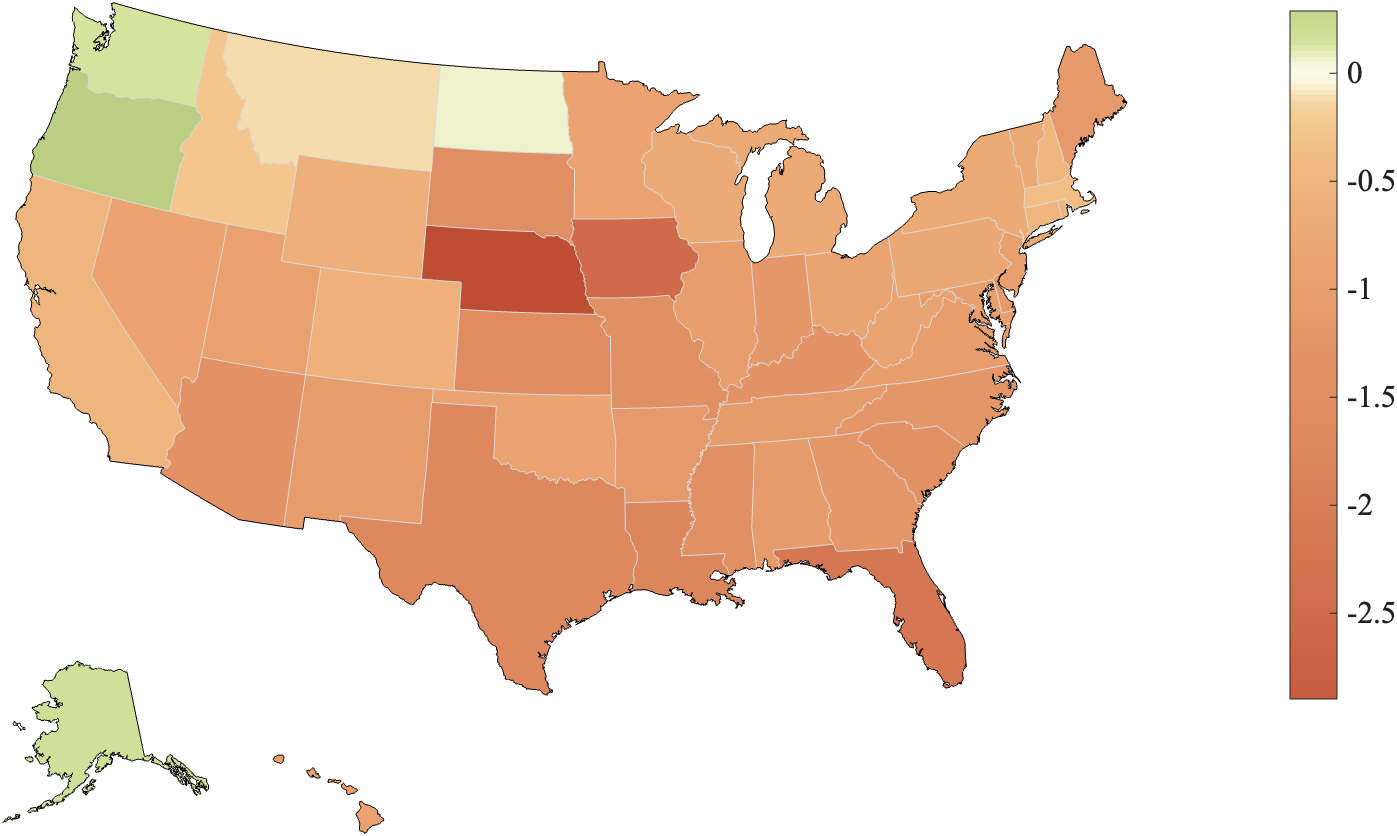
\includegraphics[width=\textwidth]{../Output/big_nu/graph_perfect_foresight/welfare_wealth_inequality_maps/welfare_wealth_inequality_maps_welfare_inequality.png}
  \end{minipage}\hfill
  \begin{minipage}[t]{0.4\textwidth}
    \centering
    \small{(b) $\Delta$ Wealth Inequality (Std Dev \%)}
    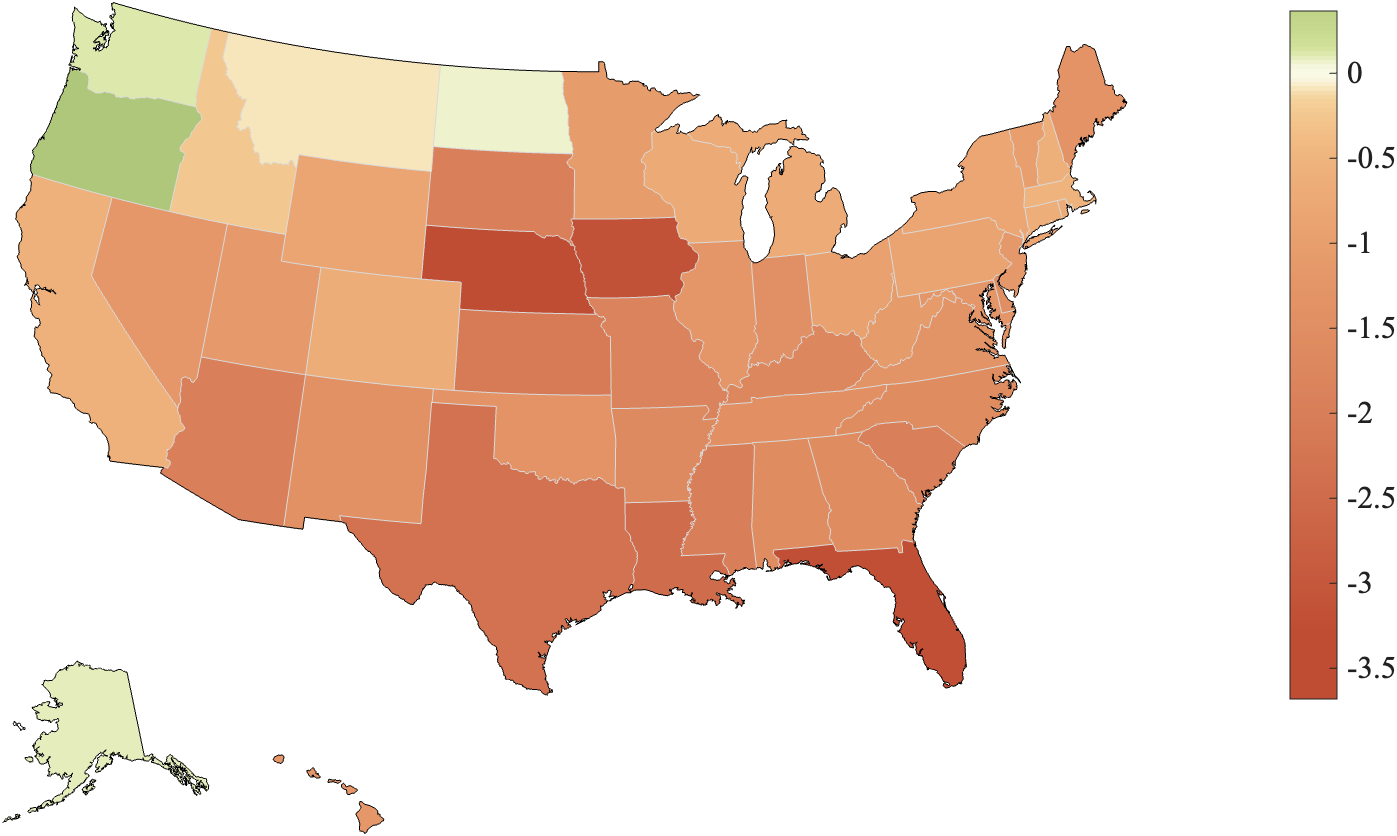
\includegraphics[width=\textwidth]{../Output/big_nu/graph_perfect_foresight/welfare_wealth_inequality_maps/welfare_wealth_inequality_maps_wealth_inequality.png}
  \end{minipage}
  \vspace{1em}
  \begin{minipage}[t]{0.4\textwidth}
    \centering
    \small{(c) Cross-State Welfare Ineq. (Time Series)}
    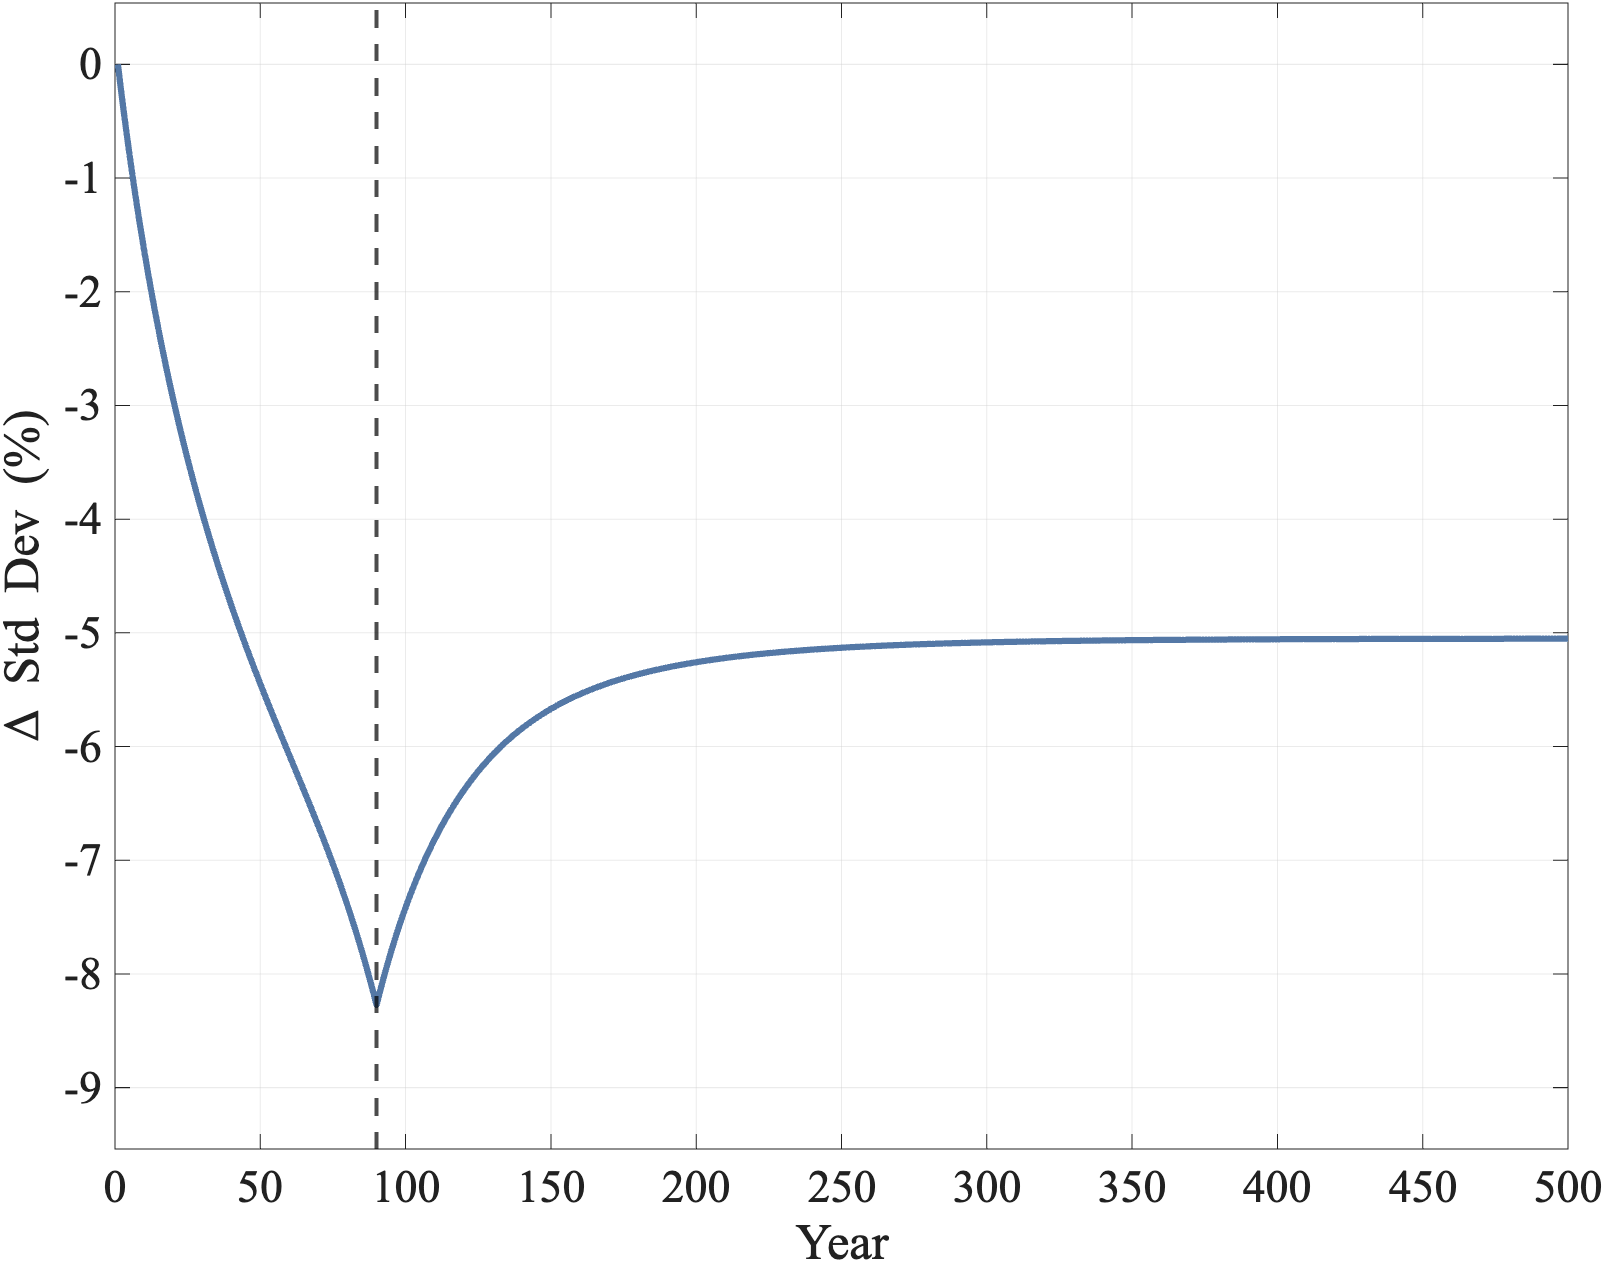
\includegraphics[width=\textwidth]{../Output/big_nu/graph_perfect_foresight/welfare_transition/welfare_transition_welfare_inequality.png}
  \end{minipage}\hfill
  \begin{minipage}[t]{0.4\textwidth}
    \centering
    \small{(d) $\Delta$ Wealth Inequality (Std Dev \%)}
    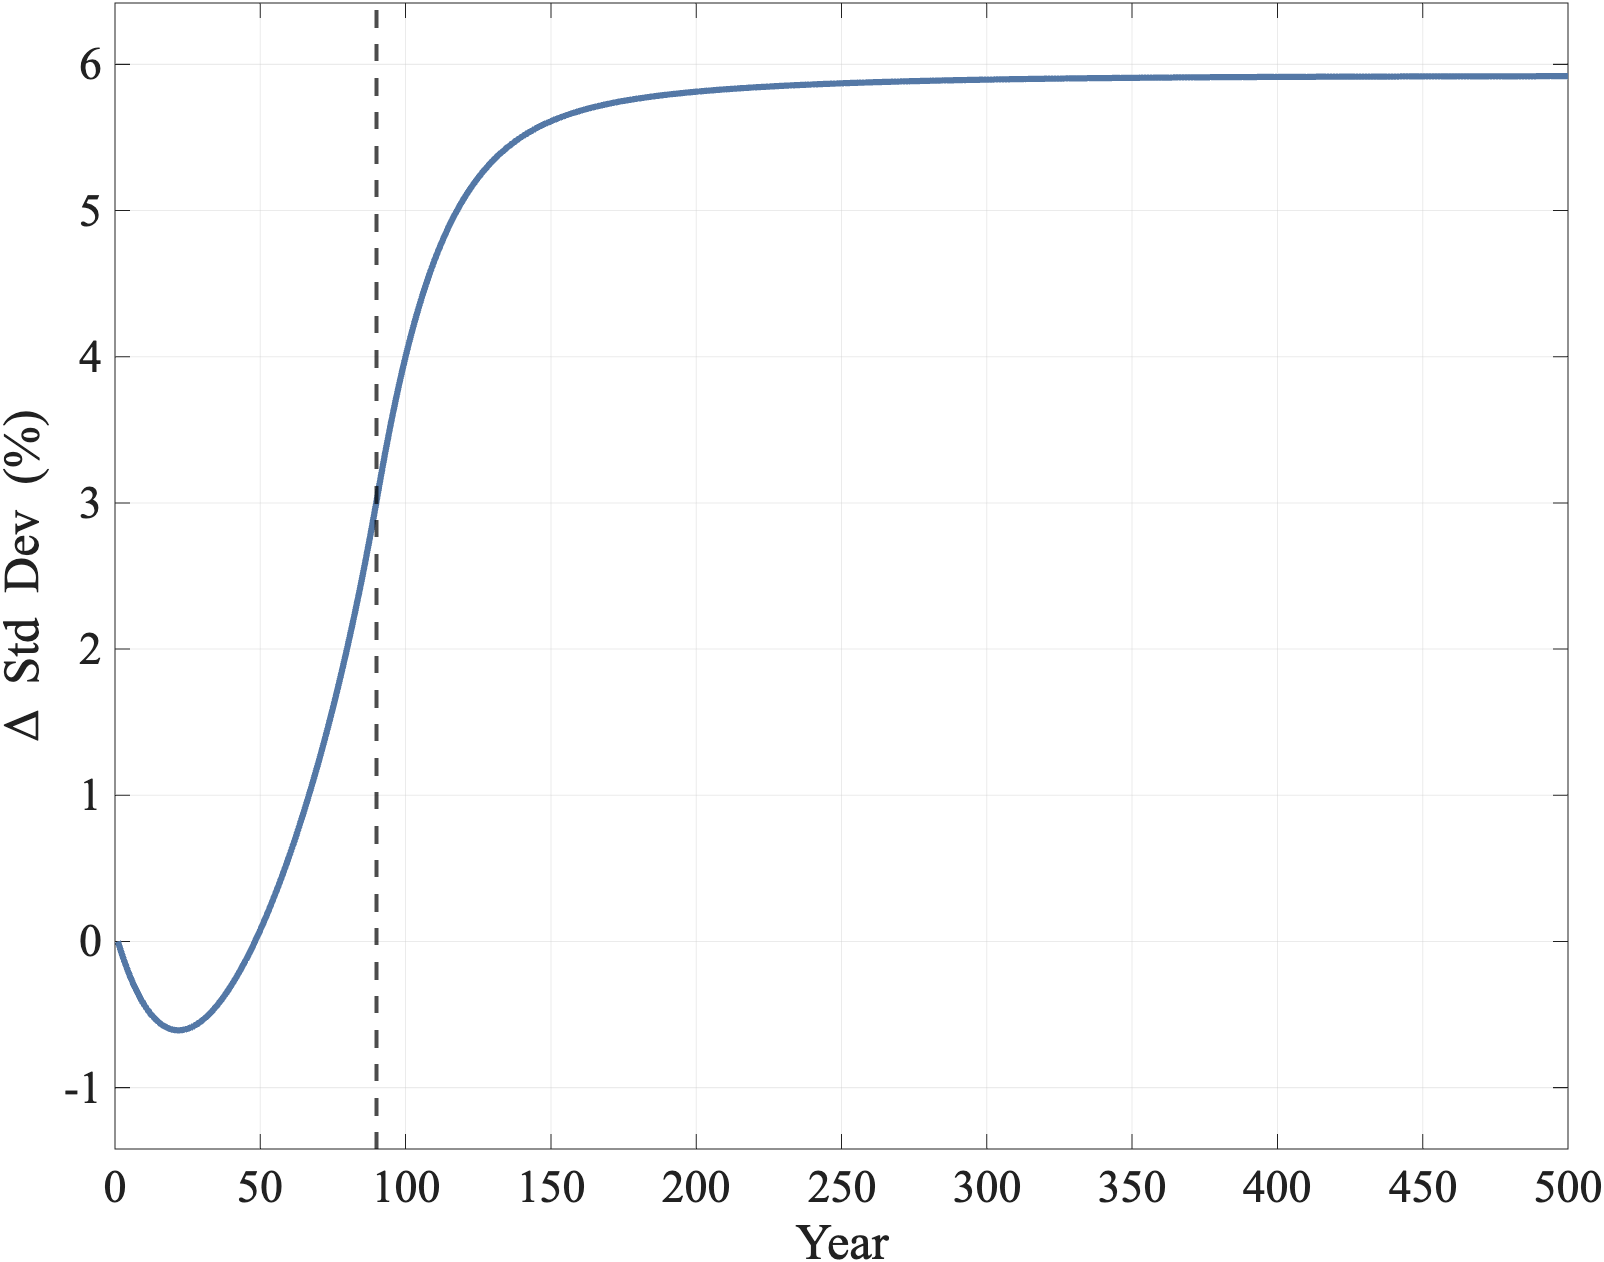
\includegraphics[width=\textwidth]{../Output/big_nu/graph_perfect_foresight/welfare_transition/welfare_transition_wealth_inequality.png}
  \end{minipage}
  \begin{minipage}{\textwidth}
  \vspace{0.5em}
  \footnotesize{\textbf{Note:} Spatial and dynamic inequality metrics under Perfect Foresight. Panel (a): percentage change in the within-state welfare standard deviation $\text{Var}_z(\text{CE}_\ell(z)) = \frac{1}{L_\ell} \sum_z \Lambda(\ell,z) [\text{CE}_\ell(z) - \overline{\text{CE}}_\ell]^2$ between the two steady states. Panel (b): percentage change in the within-state wealth standard deviation $\text{Var}_z(\bar{a}_\ell(z)) = \frac{1}{L_\ell} \sum_z \Lambda(\ell,z) [\bar{a}_\ell(z) - \bar{a}_\ell]^2$ between the two steady states. Panel (c): dynamic transition of national cross-state welfare inequality $\text{Ineq}_t^{\text{CE}} = \sum_\ell p_{\ell,t} [\overline{\text{CE}}_{\ell,t} - \overline{\text{CE}}_t^{\text{agg}}]^2$. Panel (d): dynamic transition of national cross-state wealth inequality $\text{Ineq}_t^{\text{W}} = \sum_\ell p_{\ell,t} [\bar{a}_{\ell,t} - \bar{a}_t^{\text{agg}}]^2$.} \end{minipage}
  \label{fig:ineq_pf}
\end{figure}

\subsection{The Importance of Forward-Looking Anticipation: Myopia Counterfactual}
\paragraph{Shutting Down Anticipation.} In the Myopia scenario, agents are assumed to be myopic and do not anticipate future climate damages. Instead, they make decisions based solely on current conditions, ignoring the expected trajectory of wages and amenities.\footnote{The algorithm therefore solves the fixed point of Equation \ref{eq:Xi} at each period independently. More details are given in Appendix~\ref{app:algorithms}.} This scenario allows me to isolate the effects of forward-looking behaviour on wealth accumulation, migration patterns, and welfare outcomes, and more broadly to assess the importance of anticipatory actions in adapting to climate change on the transition path in terms of speed of adjustment and negative welfare effects before reaching the new steady state. Note that without perfect foresight, the economy still reaches the same terminal steady state, but via a different transition path. Figure~\ref{fig:trans_dyn_myopia} displays the time series for the Myopia scenario.

\begin{figure}[!htb]
  \centering
  \caption{Dynamic Moments (Myopia)}
  \begin{minipage}[t]{0.4\textwidth}
    \centering
    \small{(a) Earnings}
    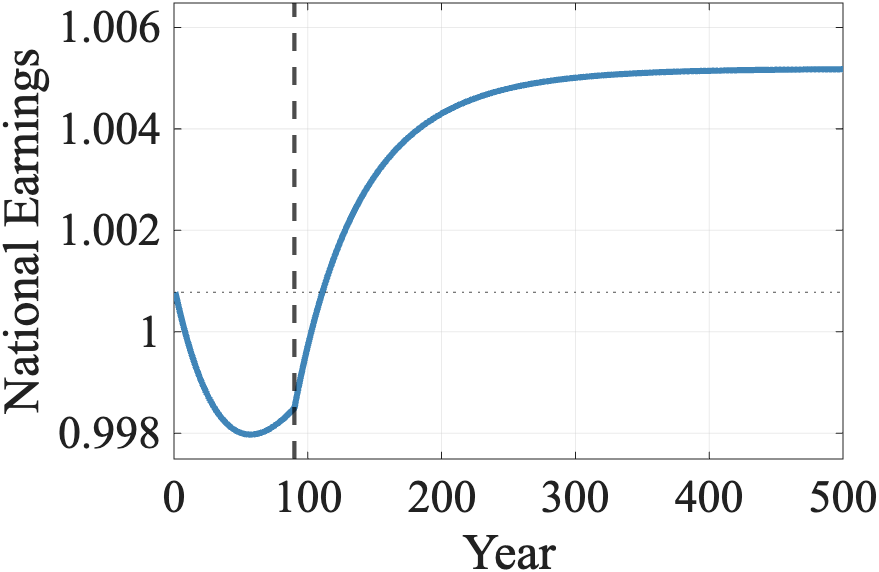
\includegraphics[width=\textwidth]{../Output/big_nu/graph_myopia/dynamic_moments/dynamic_moments_national_earnings.png}
  \end{minipage}\hfill
  \begin{minipage}[t]{0.4\textwidth}
    \centering
    \small{(b) Mobility}
    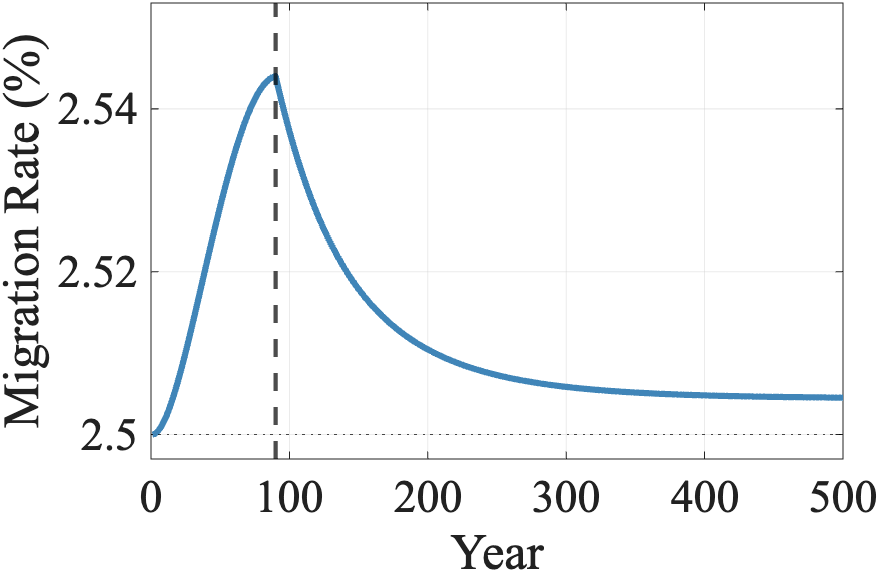
\includegraphics[width=\textwidth]{../Output/big_nu/graph_myopia/dynamic_moments/dynamic_moments_national_mobility.png}
  \end{minipage} \\[2ex]
  \begin{minipage}[t]{0.4\textwidth}
    \centering
    \small{(c) Wealth}
    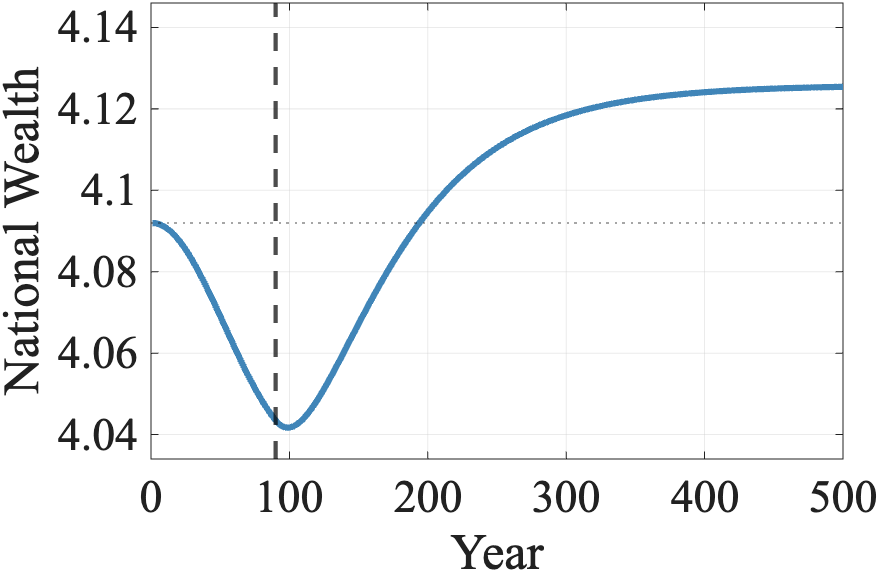
\includegraphics[width=\textwidth]{../Output/big_nu/graph_myopia/dynamic_moments/dynamic_moments_national_wealth.png}
  \end{minipage}\hfill
  \begin{minipage}[t]{0.4\textwidth}
    \centering
    \small{(d) W/Y Ratio}
    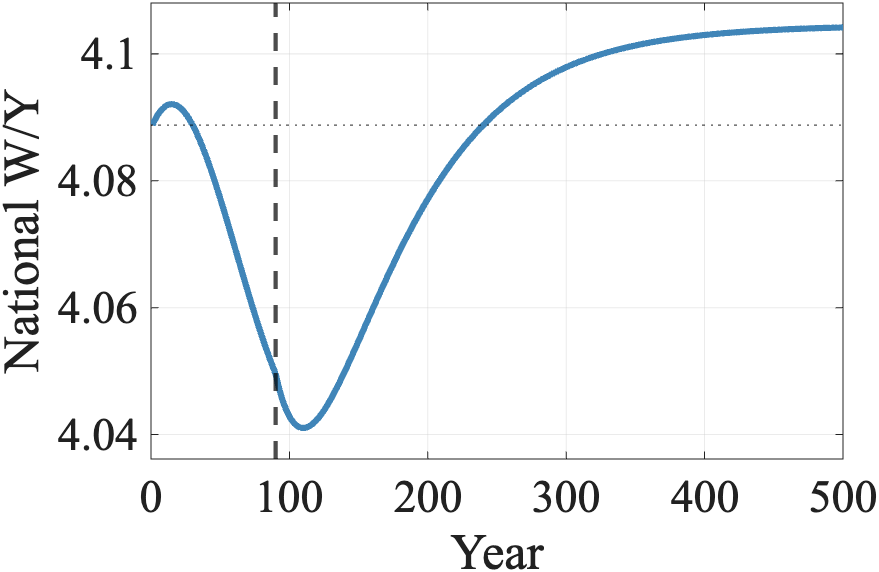
\includegraphics[width=\textwidth]{../Output/big_nu/graph_myopia/dynamic_moments/dynamic_moments_national_wy.png}
  \end{minipage}
  \begin{minipage}{\textwidth}
  \vspace{0.5em}
  \footnotesize{\textbf{Note:} Aggregate macroeconomic time series under Myopia, 2010--2500+. Agents optimise assuming current parameters persist indefinitely, solving value indices $\boldsymbol{\Xi}_t^{\text{myopia}}$ as static fixed points at each period $t$ without backward induction. Panel (a): national total disposable earnings $Y_t = \sum_{\ell,z} \tilde{w}_{\ell,t} (L_{\ell,t} + z \Lambda_t(\ell,z))$. Panel (b): national gross annual migration rate $m_t = \sum_{\ell,z} \Lambda_t(\ell,z) [1 - \mu_{\ell \ell,t}(z)] / \sum_\ell L_{\ell,t}$. Panel (c): national wealth mass $W_t = \sum_{\ell,z} \bar{a}_t(\ell,z) \Lambda_t(\ell,z)$. Panel (d): wealth-to-earnings ratio $(W/Y)_t = W_t / Y_t$.} \end{minipage}
  \label{fig:trans_dyn_myopia}
\end{figure}

Aggregate earnings and the inter-state migration rate follow roughly the same trajectory as in the baseline scenario, only with a slight delay (the migration rate peaks in 2100 in the Myopia scenario, compared to 2090 in the baseline). More importantly, because there is no anticipation of future damages, agents do not engage in precautionary saving to smooth the expected gradual drop in wages and amenities. Between 2010 and 2100, aggregate wealth and the wealth-to-income ratio decrease. As agents are hit by progressive climate damages that they fail to anticipate, they treat each successive deterioration as an unexpected, permanent shock, forcing them to consume out of their wealth rather than accumulate savings in anticipation. This lack of preparation has negative welfare consequences along the transition path: the welfare drop by 2100 in the Myopia scenario is four times larger than in the baseline scenario. After 2100, once climate fundamentals stabilise, workers find their asset holdings are below the new steady-state target. They must gradually increase their saving rate to rebuild their precautionary saving, causing aggregate wealth and the wealth-to-income ratio to slowly recover towards the new steady state. 

Finally, the speed of convergence to the new steady state is significantly slower under myopia. The transition takes approximately 400 periods (years), compared to 300 periods in the baseline scenario. This slower convergence occurs because agents enter the post-2100 period with depleted wealth and must spend decades adjusting their saving behaviour \textit{ex post} to rebuild precautionary balances, rather than accumulating them smoothly \textit{ex ante}. The transition path is therefore longer and more costly in welfare terms.

\subsection{Evaluating Adaptive Margins: Counterfactual Analysis}
To assess the importance of migration and saving in the model, I conduct two counterfactual scenarios: one where migration is suppressed and another where saving is suppressed. These counterfactuals allow me to isolate the effects of these mechanisms on wealth accumulation, migration patterns, and welfare outcomes.

\subsubsection*{\large Counterfactual 1: Suppressing Spatial Mobility (Autarky)}
\begin{figure}[!htb]
  \centering
  \caption{Dynamic Moments Levels (No Migration)}
  \label{fig:no_migration_levels}
  \begin{minipage}[t]{0.45\textwidth}
    \centering
    \small{(a) $\Delta$ Wealth (from $t=1$)}
    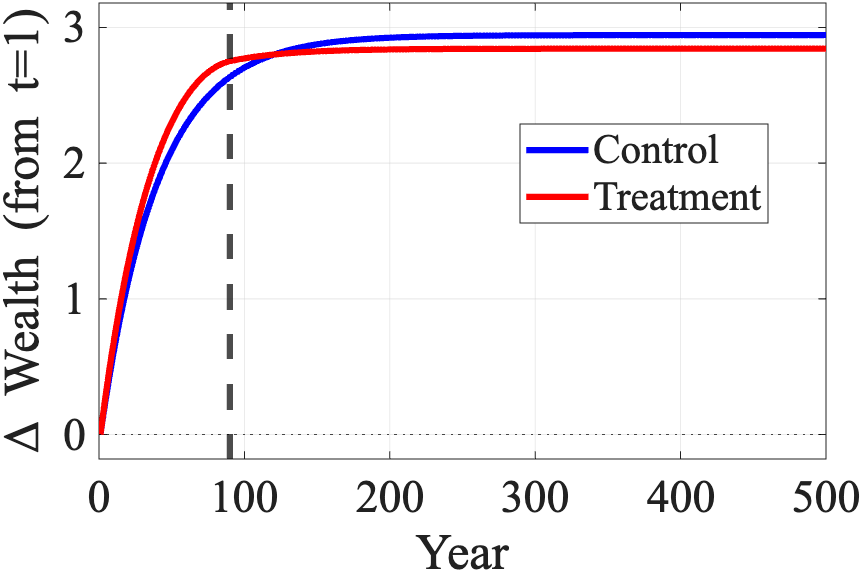
\includegraphics[width=\textwidth]{../Output/big_nu/graph_no_migration_did/did_dynamic_moments_levels_wealth.png}
  \end{minipage}\hfill
  \begin{minipage}[t]{0.45\textwidth}
    \centering
    \small{(b) $\Delta$ W/Y (from $t=1$)}
    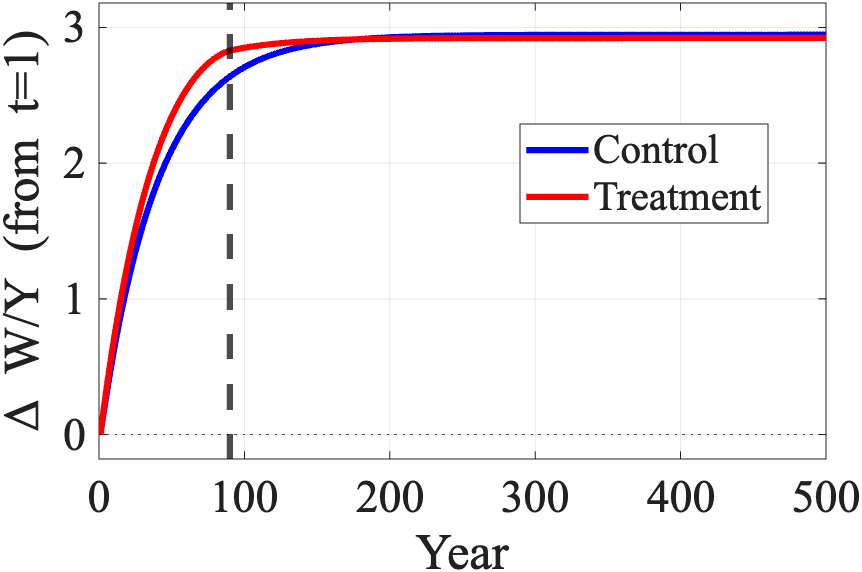
\includegraphics[width=\textwidth]{../Output/big_nu/graph_no_migration_did/did_dynamic_moments_levels_wy.png}
  \end{minipage}
  \begin{minipage}{\textwidth}
  \vspace{0.5em}
  \footnotesize{\textbf{Note:} Evolution of aggregate wealth and wealth-to-income ratio in levels (relative to $t=1$) under No Migration for both Treatment and Control groups. By tracking the levels alongside the differences, we isolate the pure local behavioural response to the climate shock.}
  \end{minipage}
\end{figure}


\paragraph{Shutting Down Migration.} In the No Migration scenario, I set the bilateral migration costs to be prohibitively high ($\psi_{j\ell} = 10^8$ for $j \neq \ell$), effectively preventing any interstate migration. Methodologically, I maintain the same initial steady state with active migration as the baseline. The economy then transitions along two distinct paths: a control path with no migration and no climate change, and a treatment path with no migration but incorporating climate change. This Difference-in-Differences (DiD) approach isolates the effect of climate change under autarky and ensures that the welfare comparisons are evaluated against a consistent initial benchmark. As explained in Section~2.3 regarding the control scenario, wealth still increases significantly due to the loss of the spatial option value, as shown by the level changes in Figure~\ref{fig:no_migration_levels}.

\begin{figure}[!htb]
  \centering
  \caption{Dynamic Moments Diff (No Migration (DiD))}
  \begin{minipage}[t]{0.4\textwidth}
    \centering
    \small{(a) Earnings Diff}
    \includegraphics[width=\textwidth]{../Output/big_nu/graph_no_migration_did/did_dynamic_moments_diff_earnings.png}
  \end{minipage}\hfill
  \begin{minipage}[t]{0.4\textwidth}
    \centering
    \small{(b) Migration Diff}
    \includegraphics[width=\textwidth]{../Output/big_nu/graph_no_migration_did/did_dynamic_moments_diff_migration.png}
  \end{minipage} \\[2ex]
  \begin{minipage}[t]{0.4\textwidth}
    \centering
    \small{(c) Wealth Diff}
    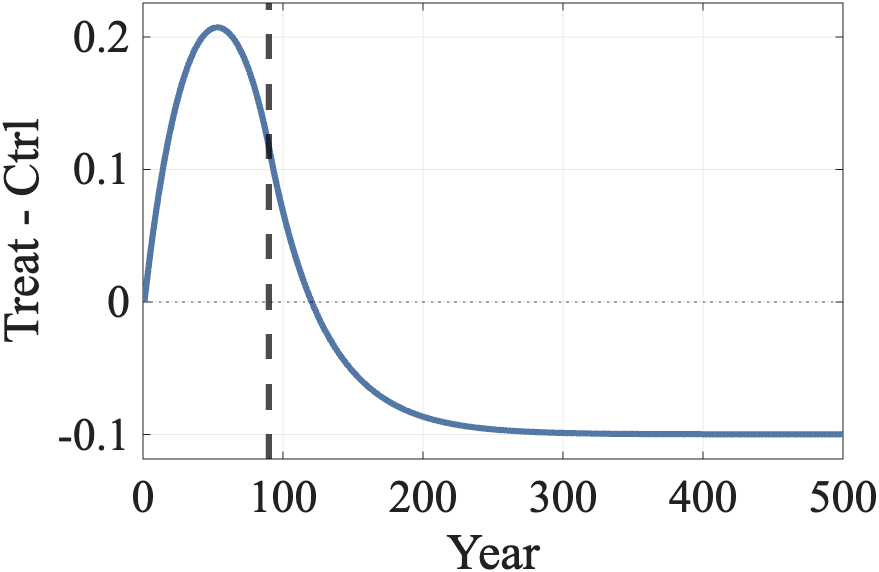
\includegraphics[width=\textwidth]{../Output/big_nu/graph_no_migration_did/did_dynamic_moments_diff_wealth.png}
  \end{minipage}\hfill
  \begin{minipage}[t]{0.4\textwidth}
    \centering
    \small{(d) W/Y Diff}
    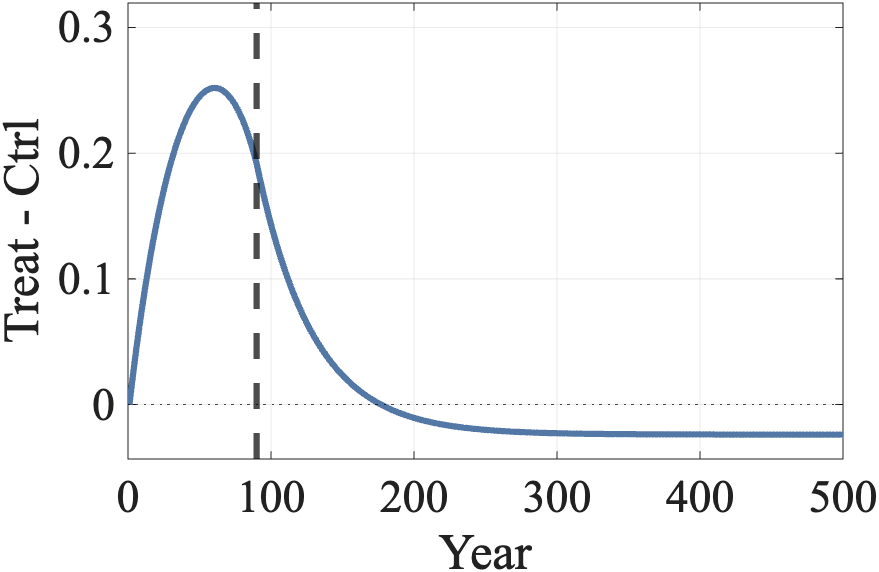
\includegraphics[width=\textwidth]{../Output/big_nu/graph_no_migration_did/did_dynamic_moments_diff_wy.png}
  \end{minipage}
  \begin{minipage}{\textwidth}
  \vspace{0.5em}
  \footnotesize{\textbf{Note:} Difference-in-Differences (DiD) macro dynamic trajectories under No Migration autarky counterfactual. Metrics measure pure climate treatment differential $\Delta^{\text{DiD}} X_t = X_t^{\text{Treat}} - X_t^{\text{Ctrl}}$ relative to zero-shock control under autarky. Panel (a): annual earnings treatment diff $\Delta^{\text{DiD}} Y_t$. Panel (b): migration treatment diff $\Delta^{\text{DiD}} m_t \equiv 0$ due to infinite moving friction. Panel (c): national wealth treatment diff $\Delta^{\text{DiD}} W_t$. Panel (d): wealth-to-earnings ratio treatment diff $\Delta^{\text{DiD}} (W/Y)_t$.} \end{minipage}
  \label{fig:dyn_mom_no_migration}
\end{figure}

\paragraph{National aggregates.} Results are shown in Figure~\ref{fig:dyn_mom_no_migration}. The migration rate is zero by construction. Aggregate earnings drop by 1.1 percent, reflecting the population-weighted average of the wage shock across states. One can observe the same wealth and wealth-to-income ratio increase before the climate shock is realised. This increase is even more pronounced than in the baseline scenario because the absence of migration amplifies the precautionary saving motive. Because agents cannot rely on relocating to less affected states, they accumulate more wealth to self-insure against the anticipated decline in wages and amenities. This amplifies the rise in the aggregate wealth and wealth-to-income ratio compared to the baseline scenario. Because there is no reallocation of population towards more productive states in the terminal steady state, the aggregate wealth and wealth-to-income ratio decline, following the aggregate earnings losses.

\begin{figure}[htb]
  \centering
  \caption{Transition Maps (No Migration)}
  \begin{minipage}[t]{0.4\textwidth}
    \centering
    \small{(a) $\Delta$ Mean Welfare (CE)}
    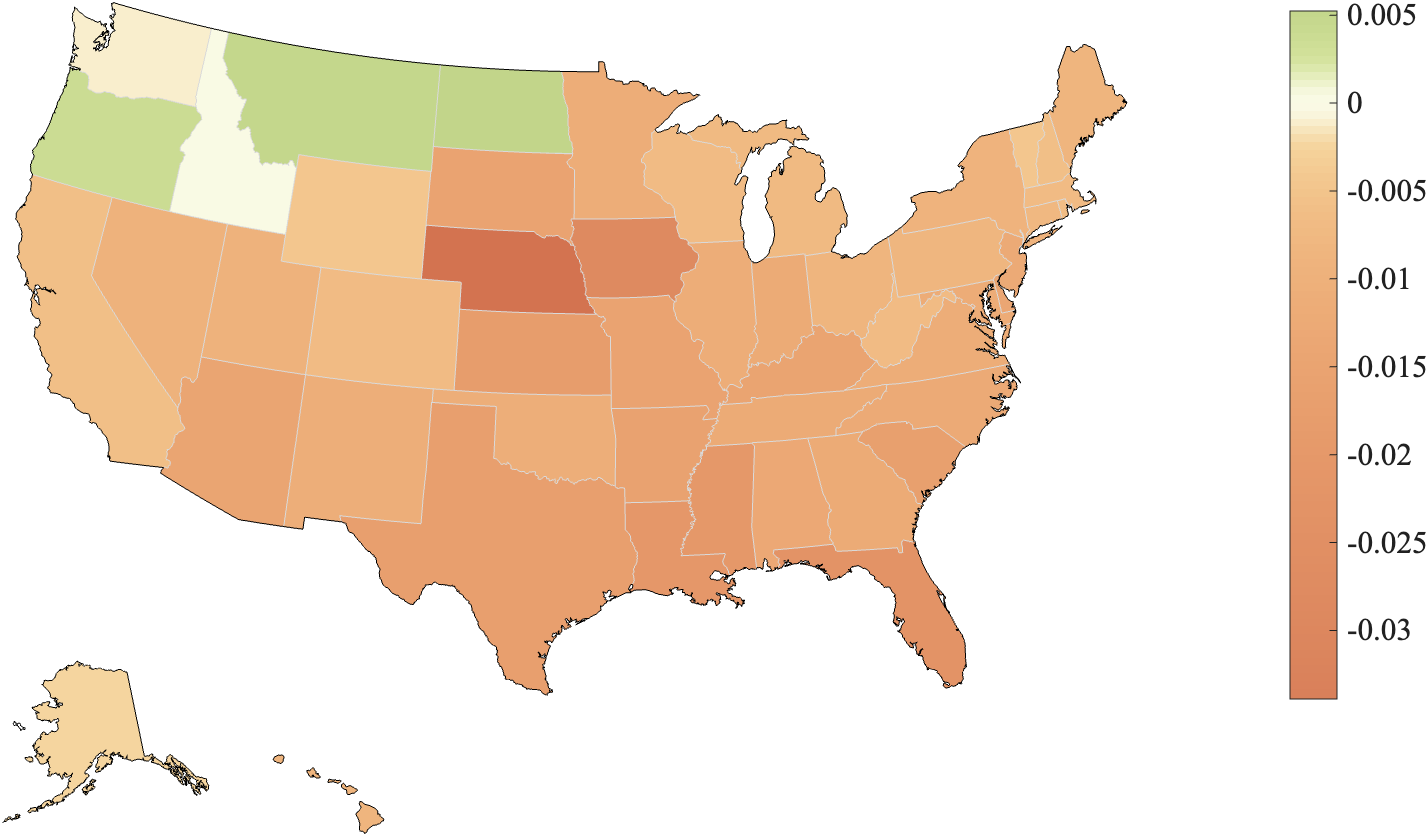
\includegraphics[width=\textwidth]{../Output/big_nu/graph_no_migration_did/transition_maps/transition_maps_delta_mean_welfare_ce.png}
  \end{minipage}\hfill
  \begin{minipage}[t]{0.4\textwidth}
    \centering
    \small{(b) $\Delta$ W/Y Ratio in level}
    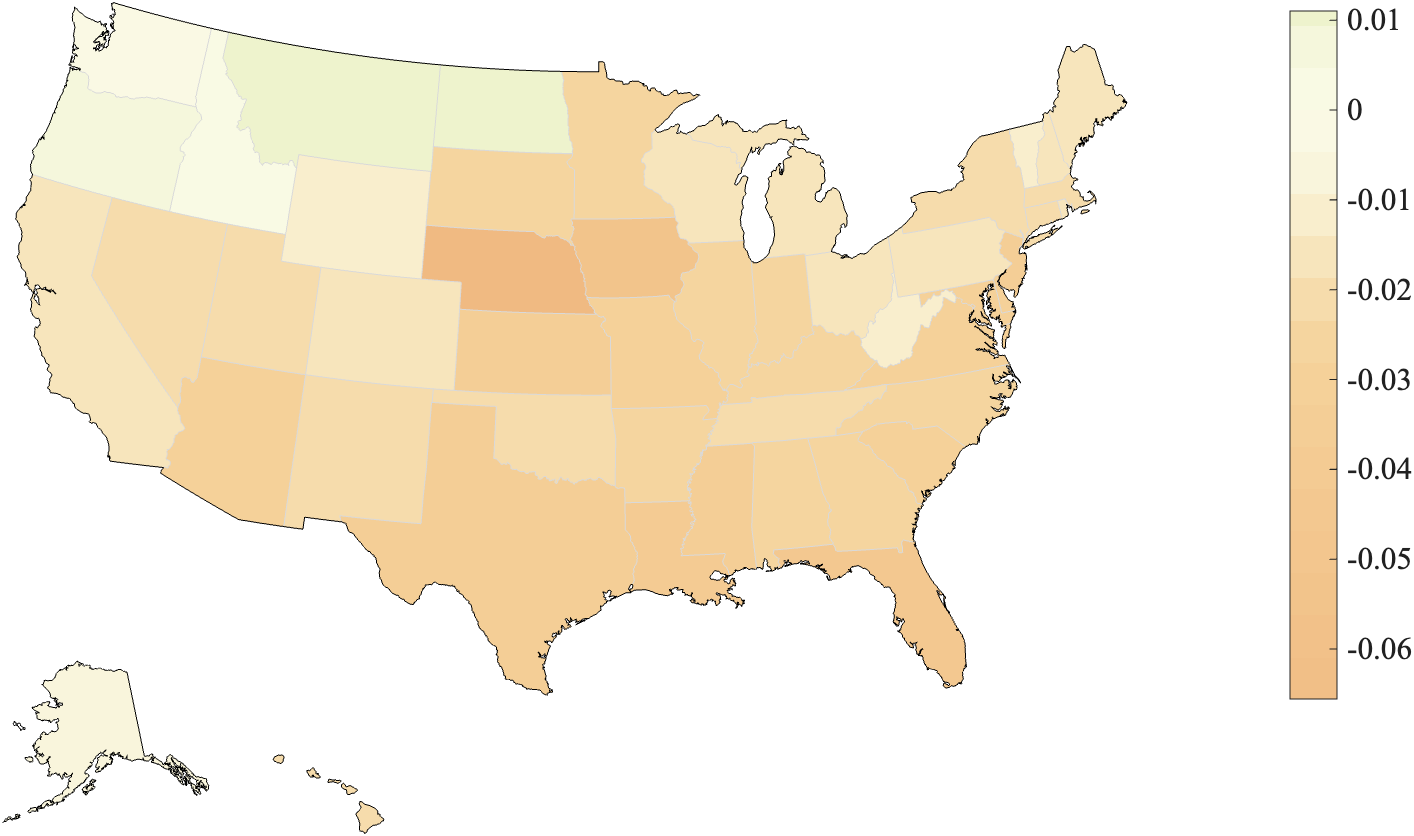
\includegraphics[width=\textwidth]{../Output/big_nu/graph_no_migration_did/transition_maps/transition_maps_wealth_income_ratio_changes.png}
  \end{minipage}
  \vspace{1em}
  \begin{minipage}[t]{0.4\textwidth}
    \centering
    \small{(c) $\Delta$ Local Population (\%)}
    \includegraphics[width=\textwidth]{../Output/big_nu/graph_no_migration_did/transition_maps/transition_maps_local_pop_changes_pct.png}
  \end{minipage}\hfill
  \begin{minipage}[t]{0.4\textwidth}
    \centering
    \small{(d) $\Delta$ Mean Wealth (\%)}
    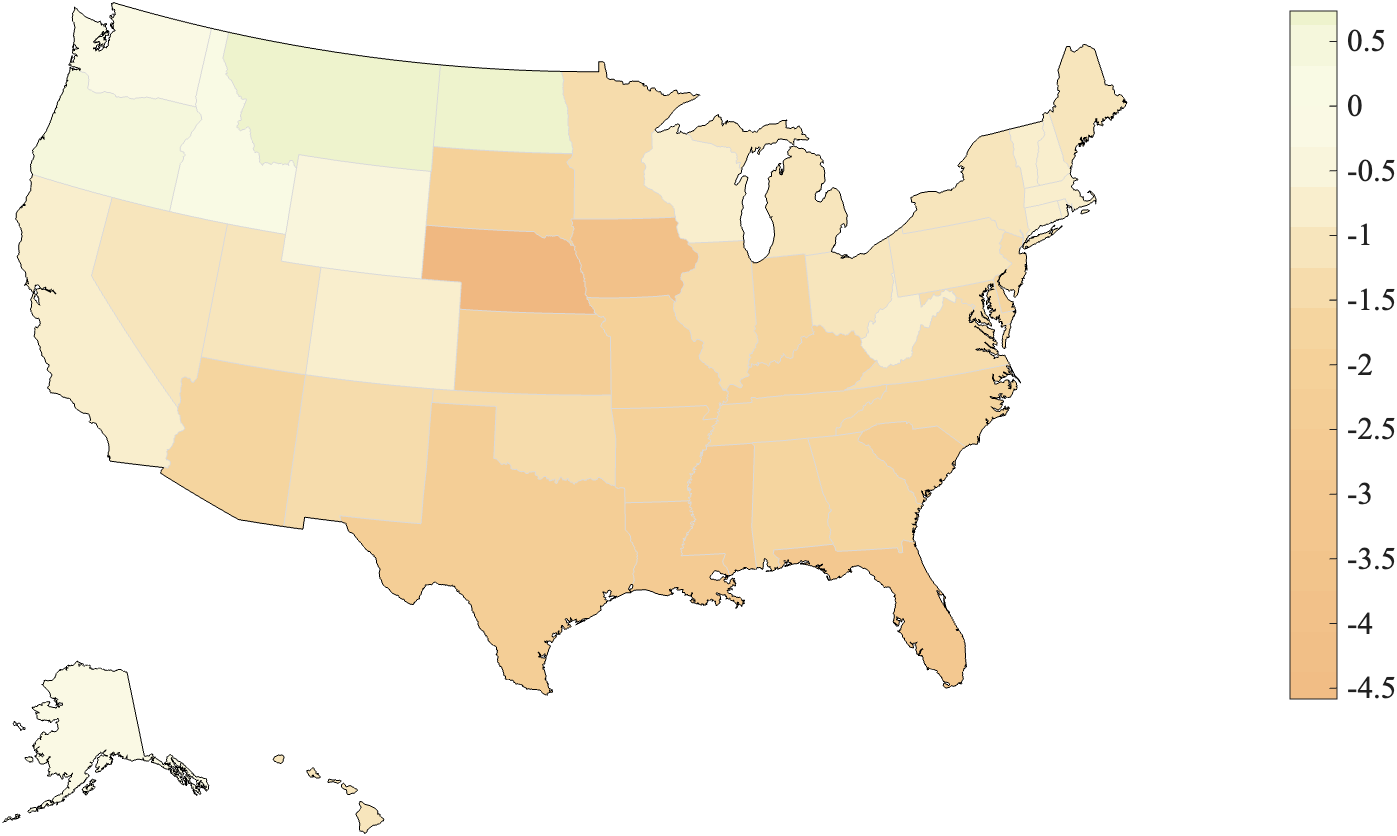
\includegraphics[width=\textwidth]{../Output/big_nu/graph_no_migration_did/transition_maps/transition_maps_pop_changes_pp.png}
  \end{minipage}
  \begin{minipage}{\textwidth}
  \vspace{0.5em}
  \footnotesize{\textbf{Note:} Spatial maps comparing the terminal steady state under 2100 climate parameters ($SS_\text{term}$) to the initial 2010 baseline steady state ($SS_\text{init}$) under No Migration autarky. Panel (a): change in mean Certainty Equivalent welfare $\Delta \text{CE}_\ell = \overline{\text{CE}}_{\ell, \text{term}} - \overline{\text{CE}}_{\ell, \text{init}}$. Panel (b): change in state wealth-to-earnings ratio $\Delta (W/Y)_\ell = (W/Y)_{\ell, \text{term}} - (W/Y)_{\ell, \text{init}}$. Panel (c): relative population change $\Delta L_\ell\% \equiv 0$. Panel (d): percentage change in state mean per-capita wealth $\Delta \bar{a}_\ell\%$.} \end{minipage}
  \label{fig:spatial_hetero_no_migration}
\end{figure}

\paragraph{Spatial heterogeneity.} Results are presented in Figure~\ref{fig:spatial_hetero_no_migration}. While the uniformity of population changes is mechanical, notably, there is very little heterogeneity in the wealth and wealth-to-income ratio changes across states. The absence of migration prevents the spatial sorting of workers based on productivity and amenities, and eliminates the influence of idiosyncratic preference shocks on spatial reallocation. This contrasts with the baseline scenario, where migration permits differential adjustments to state-level climate damages and amenities. This mechanism impacts the wealth decomposition shown in Figure~\ref{fig:wealth_decomp_no_migration}. The spatial option value, transition, and composition margins are entirely absent. Changes in wealth are driven uniquely by the damage-dampening and risk margins, which affect states more uniformly. The absence of migration yields a more homogeneous distribution of wealth and income losses which shows how, in response to climate change, migration amplifies spatial heterogeneity and exhibits the complementarity between saving and migration. Without migration as an adaptive mechanism, the economy experiences a more pronounced decline in welfare, as agents cannot escape the negative effects of climate change by moving to less affected states. Figure \ref{fig:welfare_comp_pc} shows that at the terminal steady state the welfare loss in the No Migration scenario is three times larger than in the baseline scenario. Nevertheless, more Northern states experience a small increase in welfare than in the baseline scenario because they are less affected by climate change and benefit from the absence of migration from Southern states (see Figure \ref{fig:spatial_hetero_no_migration}).

\begin{figure}[!htb]
  \centering
    \caption{Wealth Decomposition (No Migration)}
  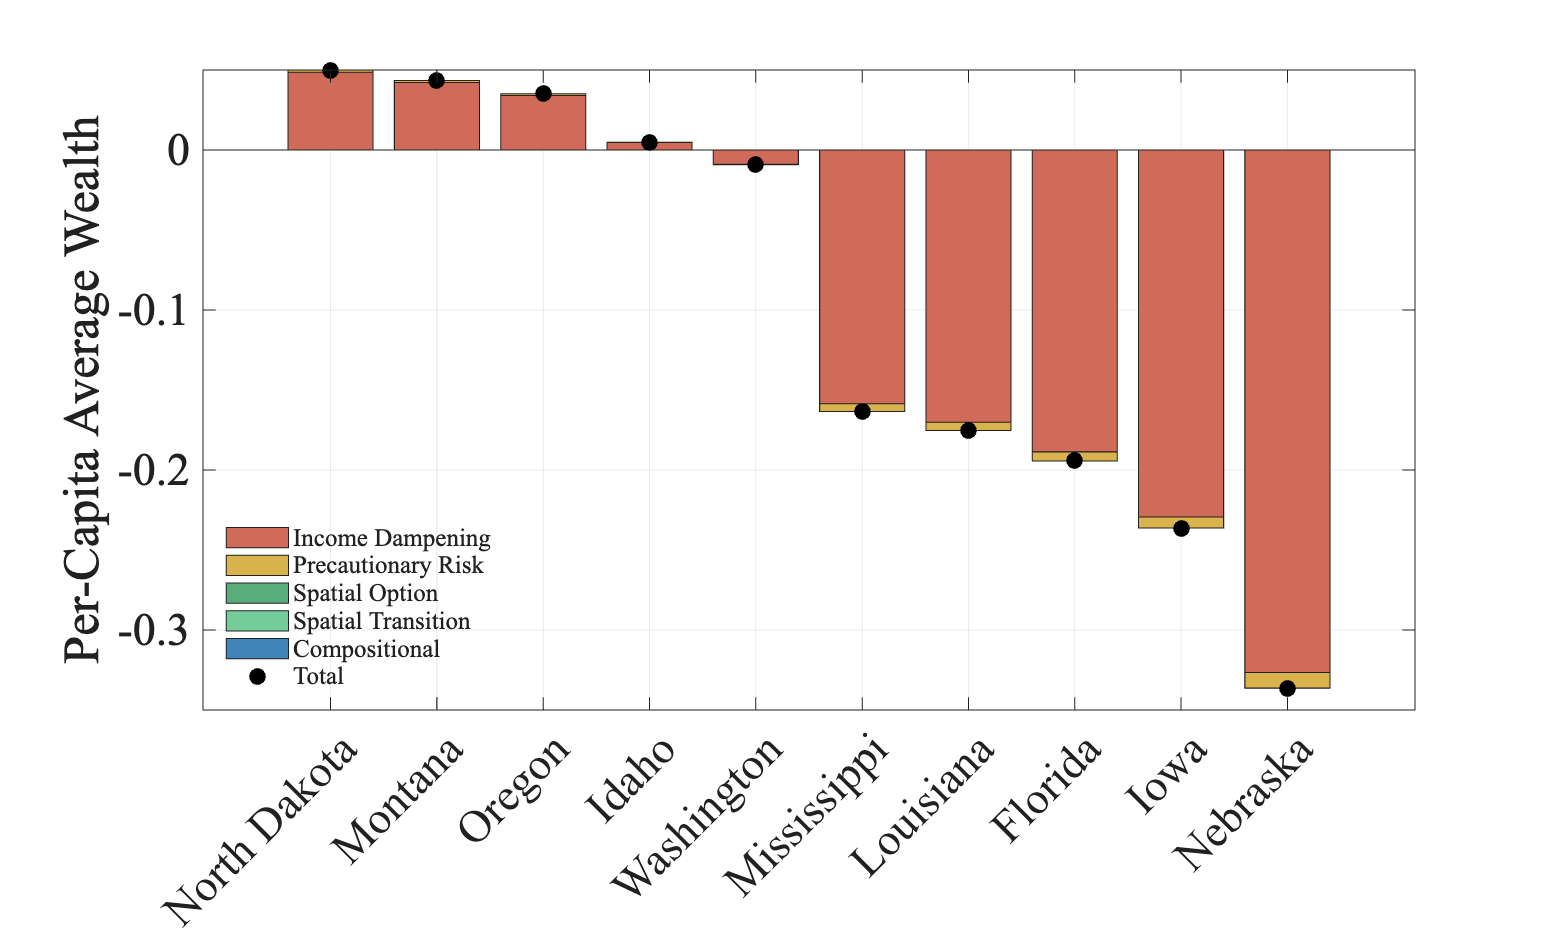
\includegraphics[width=\textwidth]{../Output/big_nu/graph_no_migration_did/exact_percapita_decomposition_bar_did_no_migration_Treat_vs_Ctrl.png}
  \begin{minipage}{\textwidth}
  \vspace{0.5em}
  \footnotesize{\textbf{Note:} Structural shift-share decomposition of the state-level per-capita wealth change $\Delta \bar{a}_\ell = \bar{a}_{\ell, \text{term}} - \bar{a}_{\ell, \text{init}}$ under No Migration into five margins: (1) Income Dampening: savings adjustments to income changes evaluated at the baseline autarky network; (2) Precautionary Risk: shifts in savings due to altered income variance evaluated at autarky; (3) Spatial option: network premium from accumulating wealth over the baseline spatial network versus autarky; (4) Spatial Transition: change in the migration network evaluated at the new savings behaviour; (5) Compositional: changes in local productivity shares. Since migration is shut down, the three spatial margins are identically zero and not represented.}
  \end{minipage}
  \label{fig:wealth_decomp_no_migration}
\end{figure}

\subsubsection*{\large Counterfactual 2: Suppressing Wealth Accumulation (Hand-to-Mouth)}
\paragraph{Shutting Down Saving} To evaluate the counterfactual scenario in which the saving mechanism is suppressed, I construct a variant of the model where agents operate as hand-to-mouth consumers. This modification is necessary because the closed-form resolution of the baseline model relies on the Euler equation that governs the optimal consumption-saving path. In this alternative framework, the core economic environment (spatial frictions, idiosyncratic preference shocks, and the income process) remains identical to the baseline. The unique change lies in the derivation of the continuation value, $\Xi_{\ell,t}(z^\prime)$, which is reconstructed to evaluate lifetime expected utility under the binding constraint that current income must be allocated to today's consumption. In this scenario, worker asset holdings $a$ are zero, and the Certainty Equivalent adjustment drops the wealth term.

In this hand-to-mouth specification, workers consume their full disposable income each period: $c_{\ell,t} = \tilde{y}_{\ell,t} + \tilde{w}_{\ell,t}z^\prime + \tilde{w}_{\ell,t}\eta^\prime$. Substituting this into the intra-period utility and applying the expectation operator over the transitory shock $\eta^\prime$, the new recursive continuation value is:

\begin{equation}
\Xi_{\ell,t}(z^\prime) = -\frac{1}{\gamma} \ln \left( \exp\left(F_{\ell,t}(z^\prime)\right) + \beta \Omega_{\ell,t}(z^\prime) \right)
\label{eq:Xi_nosaving}
\end{equation}

where $F_{\ell,t}(z^\prime)$ is the flow utility from consuming today's income:
\begin{equation}
F_{\ell,t}(z^\prime) = -\gamma \tilde{y}_{\ell,t} - \gamma \tilde{w}_{\ell,t} z^\prime - \tilde{A}_{\ell,t} + \frac{1}{2}(\gamma \tilde{w}_{\ell,t})^2 \sigma_{\eta,\ell}^2
\end{equation}

and $\Omega_{\ell,t}(z^\prime)$ is the spatial value capturing the option to migrate in the subsequent period, incorporating the extreme value preference shocks:
\begin{equation}
\Omega_{\ell,t}(z^\prime) = \bar{\lambda} \left[ \frac{1}{J} \sum_{m=1}^J e^{-\nu \psi_{\ell m}} \left( \mathbb{E}_{z^{\prime\prime}|z^\prime, m} \left[ e^{-\gamma \Xi_{m,t+1}(z^{\prime\prime})} \right] \right)^{-\nu} \right]^{-1/\nu}
\end{equation}
Note that in Equation \ref{eq:Xi_nosaving}, the exponentiated flow utility ($e^{F_{\ell,t}}$) and the continuation value ($\Omega_{\ell,t}$) are additive in the levels of the value function. This additive structure reflects the hand-to-mouth nature of consumption, where current income is fully consumed and does not contribute to future utility through saving. Then taking the logarithm to solve for $\Xi$ forces them into a non-linear log-sum. Whereas, Equation \ref{eq:Xi}, in the baseline, yields a multiplicative aggregation in levels, keeping $\Xi$ additively separable (affine). The full derivation of this equation is provided in Appendix~\ref{app:proofs}.

\begin{figure}[!htb]
  \centering
  \caption{Dynamic Moments (No Saving)}
  \begin{minipage}[t]{0.4\textwidth}
    \centering
    \small{(a) Earnings}
    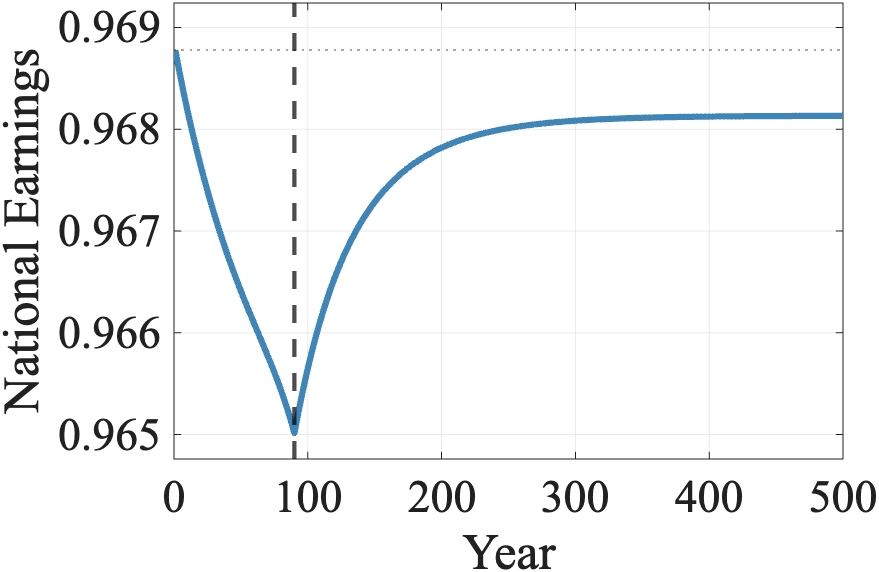
\includegraphics[width=\textwidth]{../Output/big_nu/graph_no_saving_struct/dynamic_moments/dynamic_moments_national_earnings.png}
  \end{minipage}\hfill
  \begin{minipage}[t]{0.4\textwidth}
    \centering
    \small{(b) Mobility}
    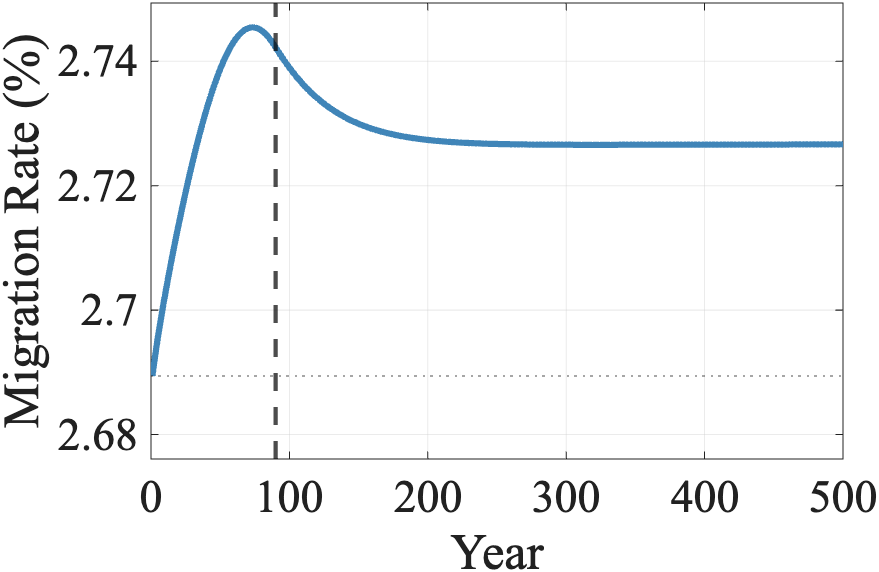
\includegraphics[width=\textwidth]{../Output/big_nu/graph_no_saving_struct/dynamic_moments/dynamic_moments_national_mobility.png}
  \end{minipage} \\[2ex]
  \begin{minipage}[t]{0.4\textwidth}
    \centering
    \small{(c) Wealth}
    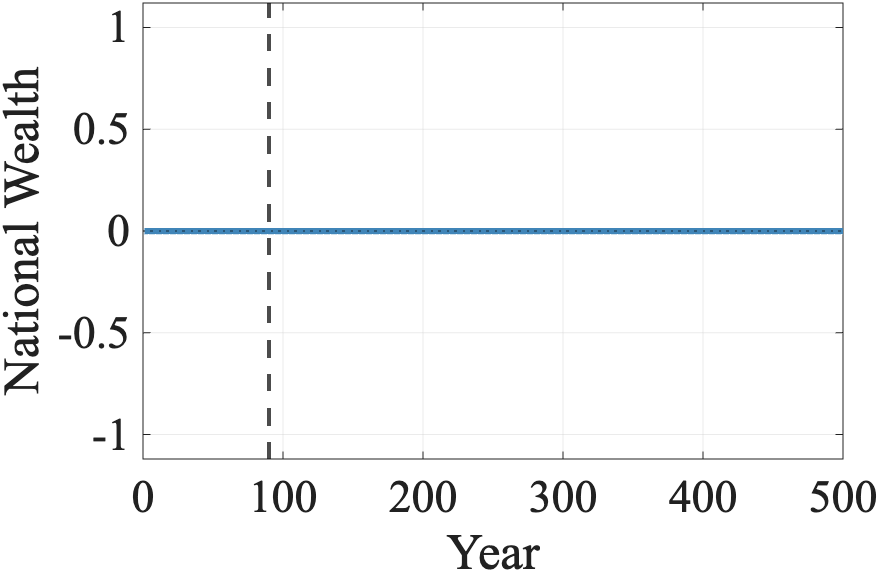
\includegraphics[width=\textwidth]{../Output/big_nu/graph_no_saving_struct/dynamic_moments/dynamic_moments_national_wealth.png}
  \end{minipage}\hfill
  \begin{minipage}[t]{0.4\textwidth}
    \centering
    \small{(d) W/Y Ratio}
    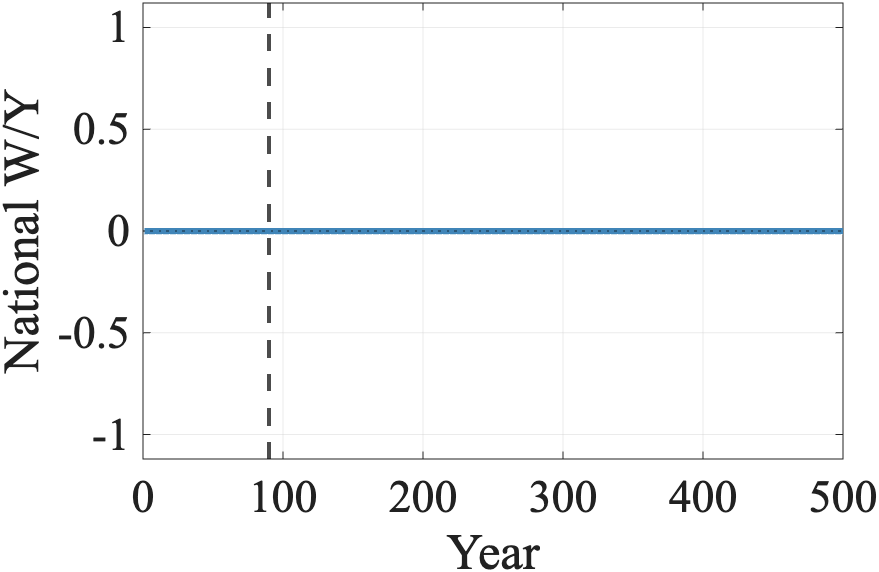
\includegraphics[width=\textwidth]{../Output/big_nu/graph_no_saving_struct/dynamic_moments/dynamic_moments_national_wy.png}
  \end{minipage}
  \begin{minipage}{\textwidth}
  \vspace{0.5em}
  \footnotesize{\textbf{Note:} Aggregate macroeconomic time series under Hand-to-Mouth workers, 2010--2500+. Workers are constrained to consume disposable income $c_t = \tilde{y}_{\ell,t}(z,\eta)$ with zero asset accumulation ($a_t \equiv 0$). Value indices solve the hand-to-mouth recursion $e^{-\gamma \Xi_\ell^{\text{NS}}(z)} = e^{F_\ell(z)} + \beta \Omega_\ell(z)$. Panel (a): national total earnings $Y_t = \sum_{\ell,z} \tilde{w}_{\ell,t} (L_{\ell,t} + z \Lambda_t(\ell,z))$. Panel (b): national gross migration rate $m_t = \sum_{\ell,z} \Lambda_t(\ell,z) [1 - \mu_{\ell \ell,t}(z)] / \sum_\ell L_{\ell,t}$. Panel (c): total wealth mass $W_t \equiv 0$. Panel (d): wealth-to-earnings ratio $(W/Y)_t \equiv 0$.} \end{minipage}
  \label{fig:dyn_mom_no_saving}
\end{figure}
\paragraph{National Aggregate.} Figure~\ref{fig:dyn_mom_no_saving} shows the national aggregate dynamics for the No Saving scenario. By default, wealth and the wealth-to-income ratio are zero. In the initial steady state, with no saving both the population distribution and the interstate migration rate change: earnings are on average lower, meaning that more people live in poorer states, which happen to be Southern States. The aggregate migration rate stands at 2.7\%, higher than the baseline. This reflects substitutability between saving and migration. Without the ability to save and thereby smooth consumption variance from idiosyncratic income shocks, workers are forced to rely on spatial mobility to smooth shocks, increasing the inter-state mobility rate. As in the baseline scenario, aggregate earnings initially decrease until 2100 before recovering to roughly their initial steady-state level, thanks to spatial reallocation. The inter-state mobility rate peaks in 2090 at roughly 2.75\% before settling at a higher terminal value. This permanent increase is driven by a compositional shift in the population. In the No Saving economy, high-wage Northern states impose a higher uninsurable variance penalty ($\frac{1}{2}(\gamma \tilde{w}_{\ell,t})^2 \sigma_{\eta,\ell}^2$) than the baseline, making them high-turnover regions, while the low-wage South acts as a low-turnover region because of a lower uninsurable variance penalty. As climate damages force population out of the Southern states and into higher-variance Northern and middle states, the national aggregate migration rate rises because a larger share of the population lives in high-turnover environments.

\paragraph{Spatial Heterogeneity.} The heterogeneity in welfare and population change is shown in Figure~\ref{fig:spatial_hetero_no_saving}. The spatial distribution of population reallocation follows the same patterns as in the baseline scenario, with Southern states losing population and Northern states gaining. However, the magnitude of this reallocation is visually less pronounced in the No Saving scenario (e.g., Florida loses approximately 60\% of its population, compared to 80\% in the baseline, while Northern states see less influx). The smaller percentage drop in the South is the result of the initial population distribution: the No Saving scenario begins with a higher Southern population base, meaning an identical absolute migratory outflow yields a smaller relative percentage decline. Second, the missing population influx to the North is driven by the uninsurable variance penalty. In a hand-to-mouth environment, agents must consume their entire income, forcing them to bear the full income variance: $\frac{1}{2}(\gamma \tilde{w}_{\ell,t})^2 \sigma_{\eta,\ell}^2$. Because this uninsurable risk premium scales with the square of the local wage, more productive Northern states become less attractive. When climate refugees flee the South, this variance penalty acts as a barrier to entry for high-wage havens, forcing migrants to disperse across sub-optimal, lower-variance states and dampening the aggregate directional reallocation.

\begin{figure}[!htb]
  \centering
  \caption{Transition Maps (No Saving)}
  \begin{minipage}[t]{0.4\textwidth}
    \centering
    \small{(a) $\Delta$ Mean Welfare (CE)}
    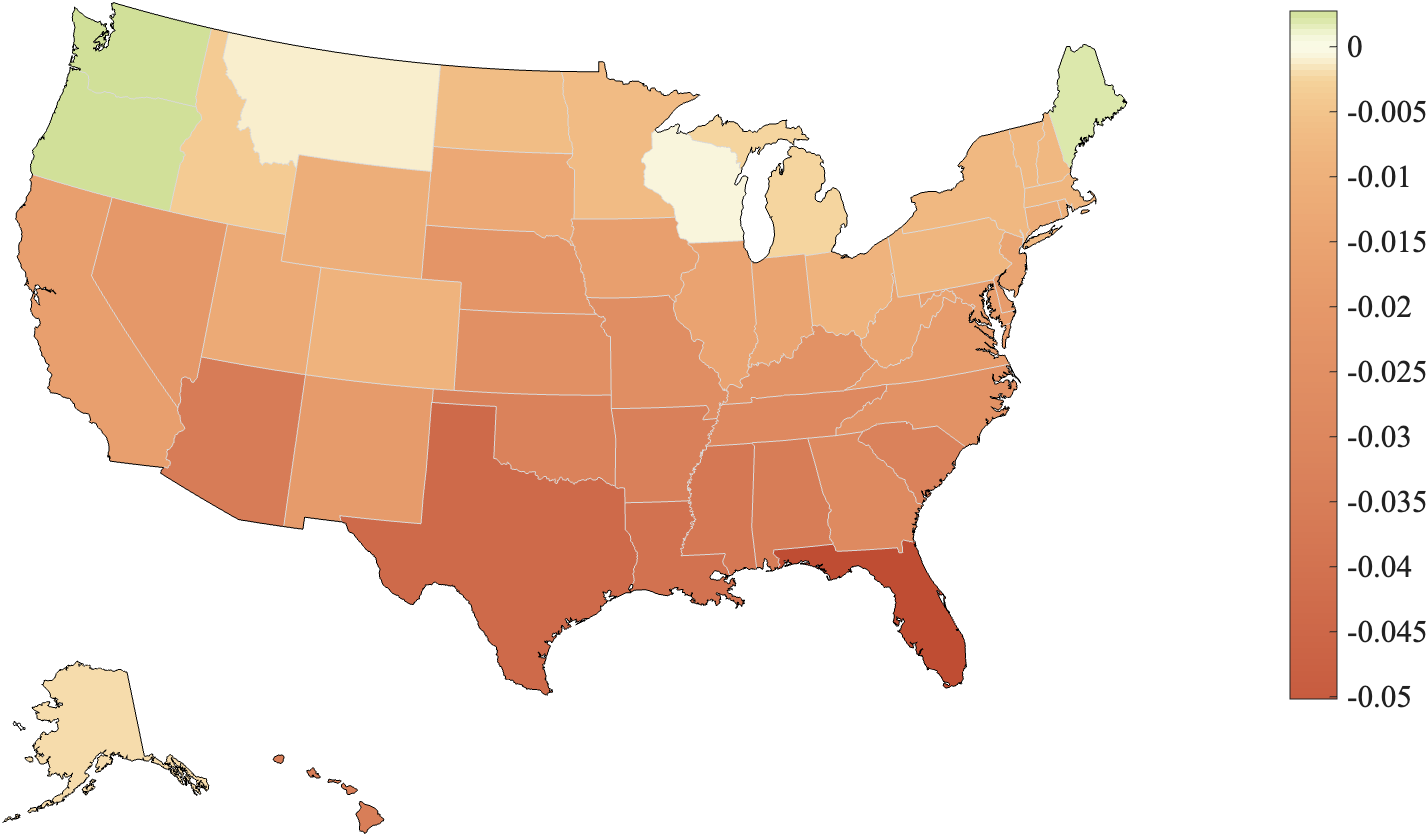
\includegraphics[width=\textwidth]{../Output/big_nu/graph_no_saving_struct/transition_maps/transition_maps_delta_mean_welfare_ce.png}
  \end{minipage}\hfill
  \begin{minipage}[t]{0.4\textwidth}
    \centering
    \small{(b) $\Delta$ Local Population (\%)}
    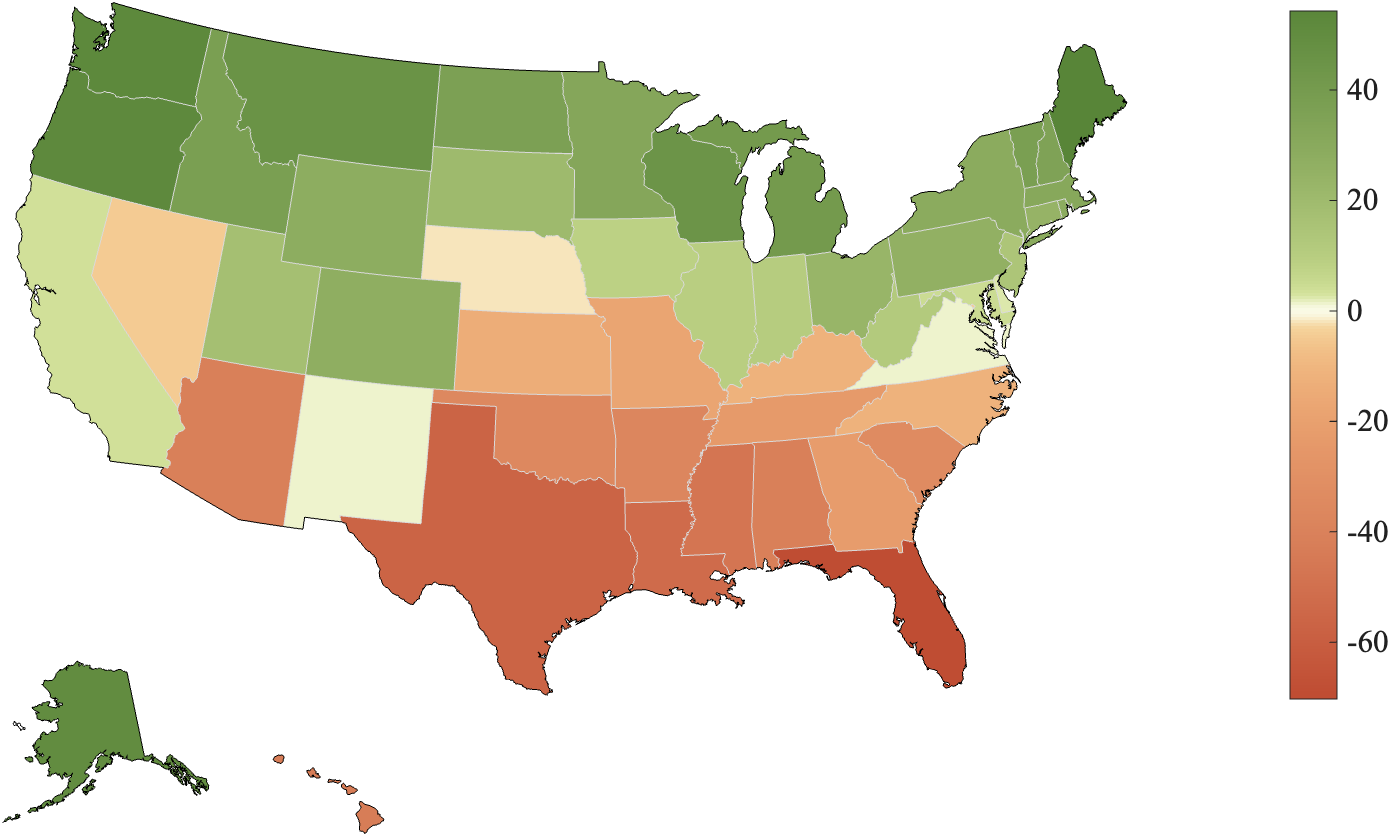
\includegraphics[width=\textwidth]{../Output/big_nu/graph_no_saving_struct/transition_maps/transition_maps_local_pop_changes_pct.png}
  \end{minipage}\hfill
  \begin{minipage}{\textwidth}
  \vspace{0.5em}
  \footnotesize{\textbf{Note:} Spatial maps comparing the terminal steady state under 2100 climate parameters ($SS_\text{term}$) to the initial 2010 baseline steady state ($SS_\text{init}$) under Hand-to-Mouth workers. Panel (a): change in mean Certainty Equivalent welfare $\Delta \text{CE}_\ell = \overline{\Xi}_{\ell, \text{term}}^{\text{NS}} - \overline{\Xi}_{\ell, \text{init}}^{\text{NS}}$, which collapses strictly to non-asset value index $\Xi^{\text{NS}}$. Panel (b): relative population percentage change $\Delta L_\ell\% = 100 \times (L_{\ell, \text{term}} - L_{\ell, \text{init}})/L_{\ell, \text{init}}$.} \end{minipage}
  \label{fig:spatial_hetero_no_saving}
\end{figure}
\paragraph{Welfare and Spatial Inequality.} Welfare losses are more pronounced in the No Saving scenario, with the national average loss reaching 2.9\% (Figure~\ref{fig:welfare_comp_pc}), compared to 0.5\% in the baseline scenario. This is due to the fact that saving allows agents to smooth unexpected shocks and climate change severely exacerbates this fragility. The spatial distribution of welfare losses follows the baseline gradient, with Southern states experiencing the most severe losses. Another result of the No Saving scenario is the asymmetric evolution of within-state welfare variance: it increases in the Southern states and decreases in the Northern states (with a +2.5 and -2.5 variation). This is a consequence of the exponential concavity of the hand-to-mouth value function.\footnote{In the baseline scenario with savings the flow utility is a constant fraction of the total value function, with Equation \ref{eq:cpol} one can show that this fraction equals $r/(1+r)$. In the No Saving scenario, the flow utility over the value function is: $ \frac{\exp(F_\ell(z))}{\exp(F_\ell(z)) + \beta \mathbb{E}[V_{\ell'}]}$, which tends towards zero for high-$z$ workers.} In the South, less productive workers are more sensitive to local flow utility and when climate damages hit, their welfare drops substantially; for high-productivity workers, they are more resilient because of the spatial option value. It widens the local welfare gap. In the North, the degradation of the spatial option value (driven by the damaged South) penalises the high-productivity workers whose welfare is heavily dominated by this option value. Because less productive workers in the North are protected from this drop by local flow utility, it equalises welfare across productivity types. Inter-state welfare's variance marginally declines.
\begin{figure}[!htb]
  \centering
  \caption{Inequality Maps and Transition (No Saving)}
  \begin{minipage}[t]{0.4\textwidth}
    \centering
    \small{(a) $\Delta$ Welfare Inequality (Std Dev \%)}
    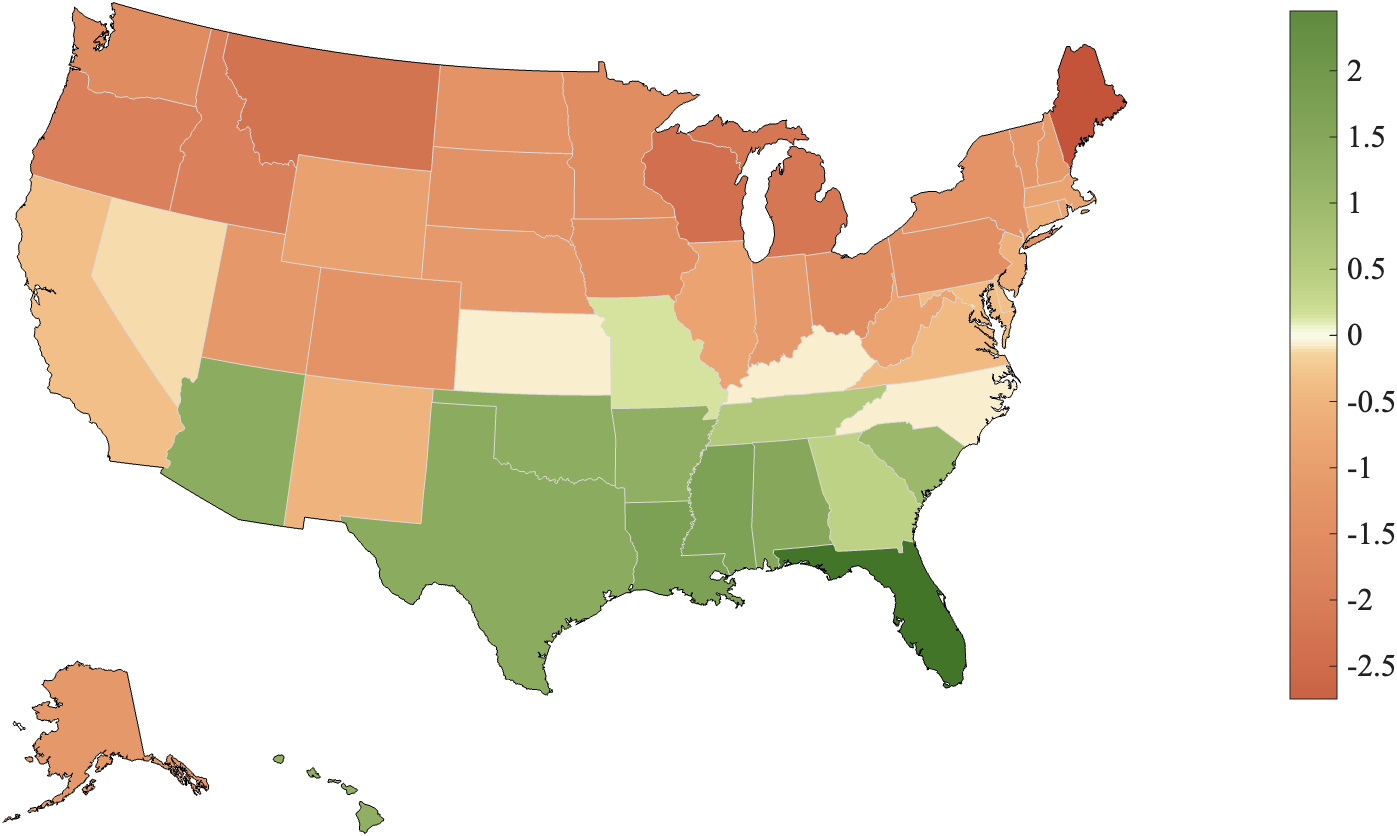
\includegraphics[width=\textwidth]{../Output/big_nu/graph_no_saving_struct/welfare_wealth_inequality_maps/welfare_wealth_inequality_maps_welfare_inequality.png}
  \end{minipage}\hfill
  \begin{minipage}[t]{0.4\textwidth}
    \centering
    \small{(b) $\Delta$ Welfare Inequality (Std Dev \%)}
    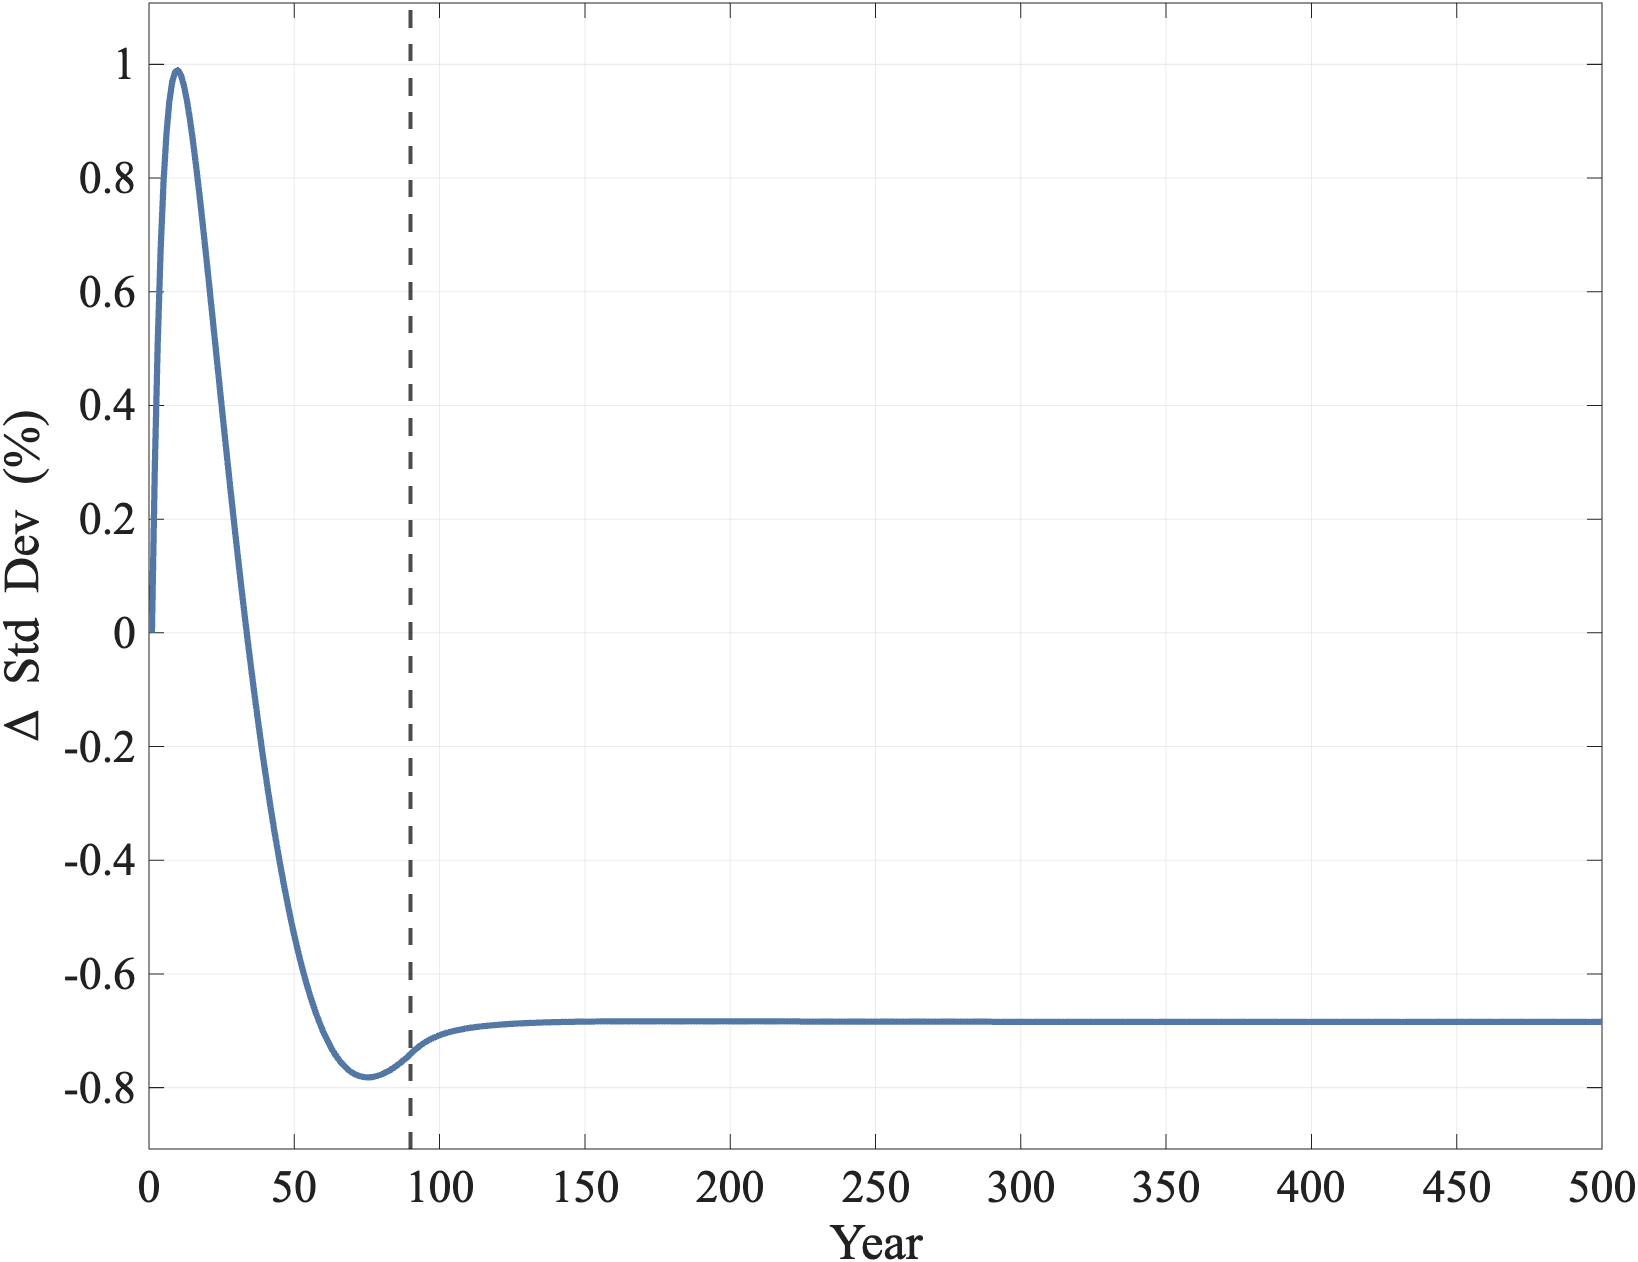
\includegraphics[width=\textwidth]{../Output/big_nu/graph_no_saving_struct/welfare_transition/welfare_transition_welfare_inequality.png}
  \end{minipage}
  \begin{minipage}{\textwidth}
  \vspace{0.5em}
  \footnotesize{\textbf{Note:} Spatial and dynamic variance metrics under Hand-to-Mouth workers. Panel (a): percentage change in the within-state welfare standard deviation $\text{Var}_z(\Xi_\ell^{\text{NS}}(z)) = \frac{1}{L_\ell} \sum_z \Lambda(\ell,z) [\Xi_\ell^{\text{NS}}(z) - \overline{\Xi}_\ell^{\text{NS}}]^2$ in 2100. Panel (b): dynamic transition of national cross-state welfare inequality $\text{Ineq}_t^{\text{CE}} = \sum_\ell p_{\ell,t} [\overline{\Xi}_{\ell,t}^{\text{NS}} - \overline{\Xi}_t^{\text{NS,agg}}]^2$.} \end{minipage}
  \label{fig:ineq_no_saving}
\end{figure}

\subsection{Cross-Scenario Analysis}
\label{sec:audit}
Figure~\ref{fig:welfare_comp_pc} presents the national aggregate dynamics for all scenarios. 
\paragraph{Earnings.}
Over all the scenarios, with the exception of the No Migration scenario, the aggregate earnings drop is low, and for the baseline it even increases by 0.4\%, which is due to the reallocation of population towards high-wage states that are less hit by climate change. The No Migration scenario shows a drop of 1.1\% in aggregate earnings, which is the population-weighted average of the wage shock across states. 
\begin{figure}[!htb]
  \centering
  \caption{Macro Comparison: Savings, Migration, Earnings, and Wealth}
  \vspace{1em}
  
  \begin{minipage}[t]{0.45\textwidth}
    \centering
    \small{(a) Earnings}
    
    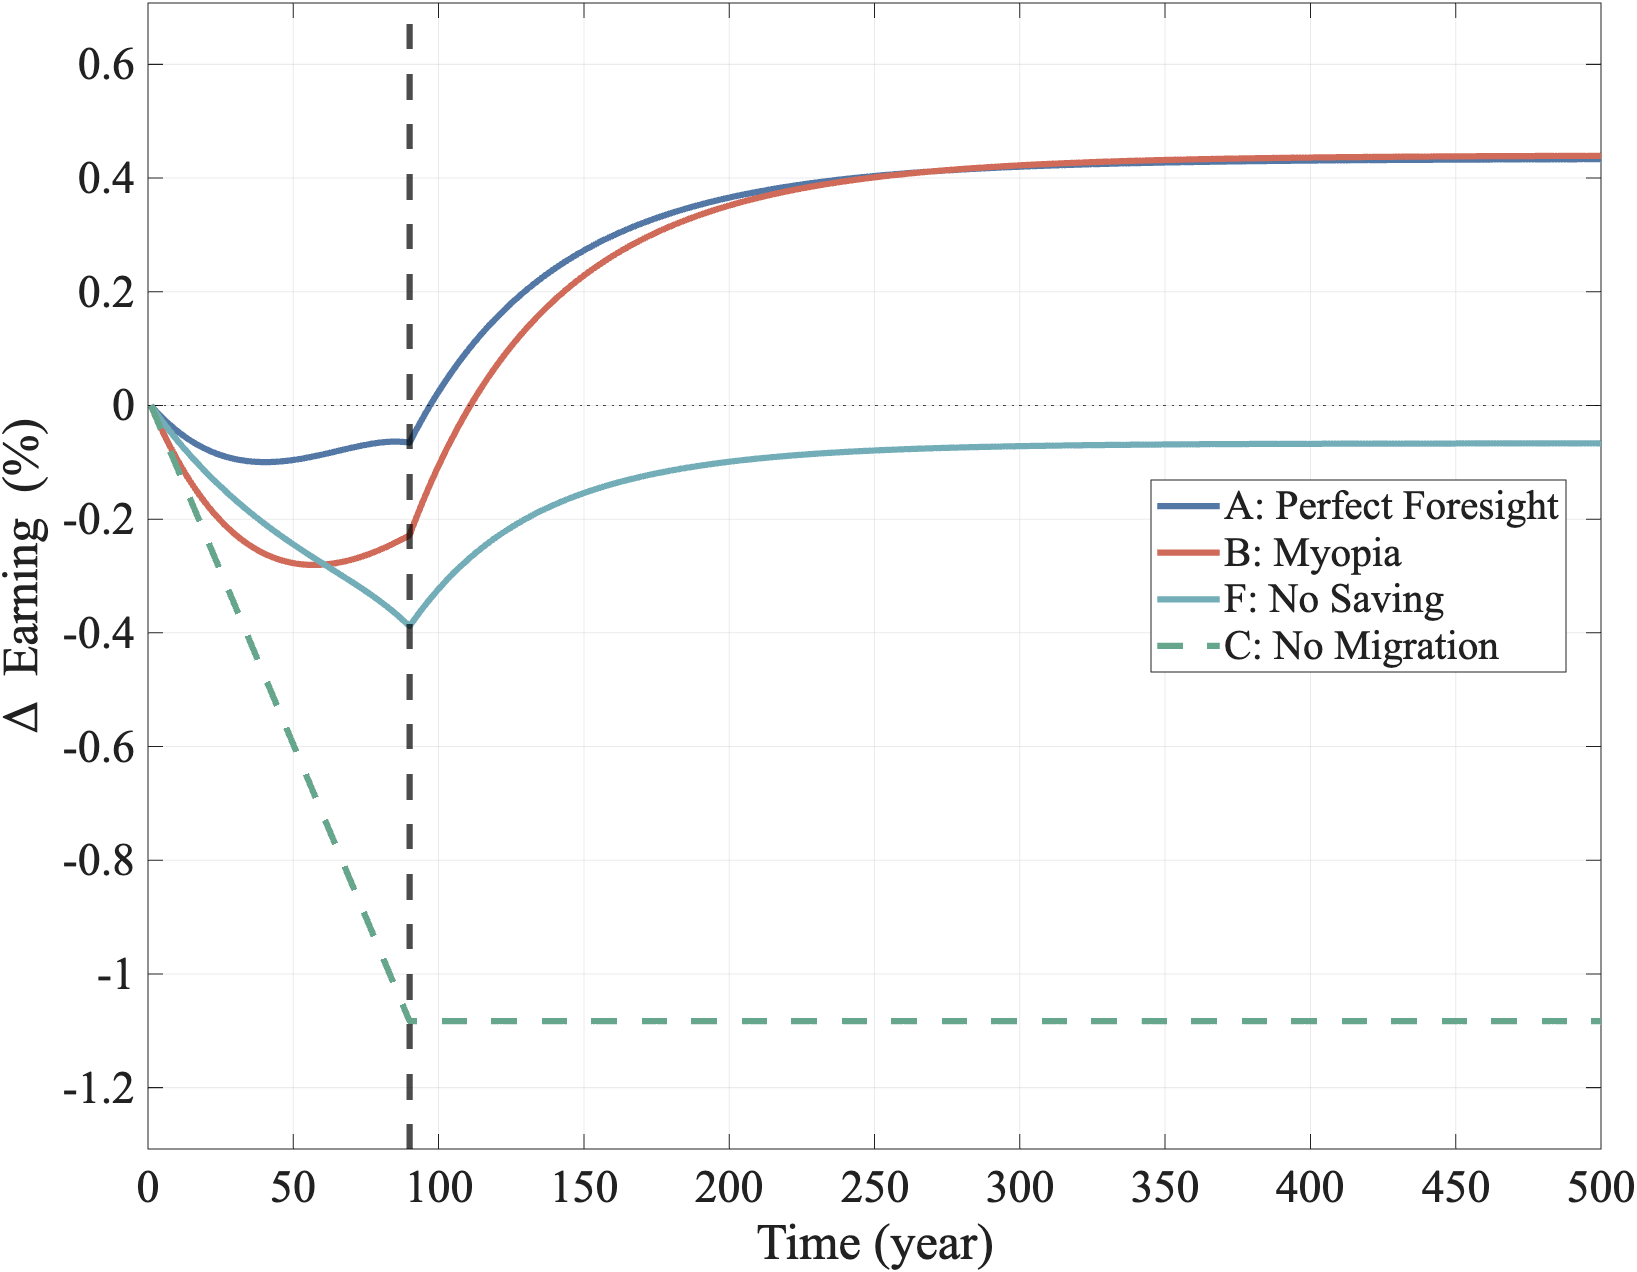
\includegraphics[width=\textwidth]{../Output/big_nu/graph_macro_audit/macro_earning_frictions/macro_earning_frictions_macro_earning_delta_earning_pc.png}
  \end{minipage}
  \hfill
  \begin{minipage}[t]{0.45\textwidth}
    \centering
    \small{(b) Wealth-to-Earnings}
    
    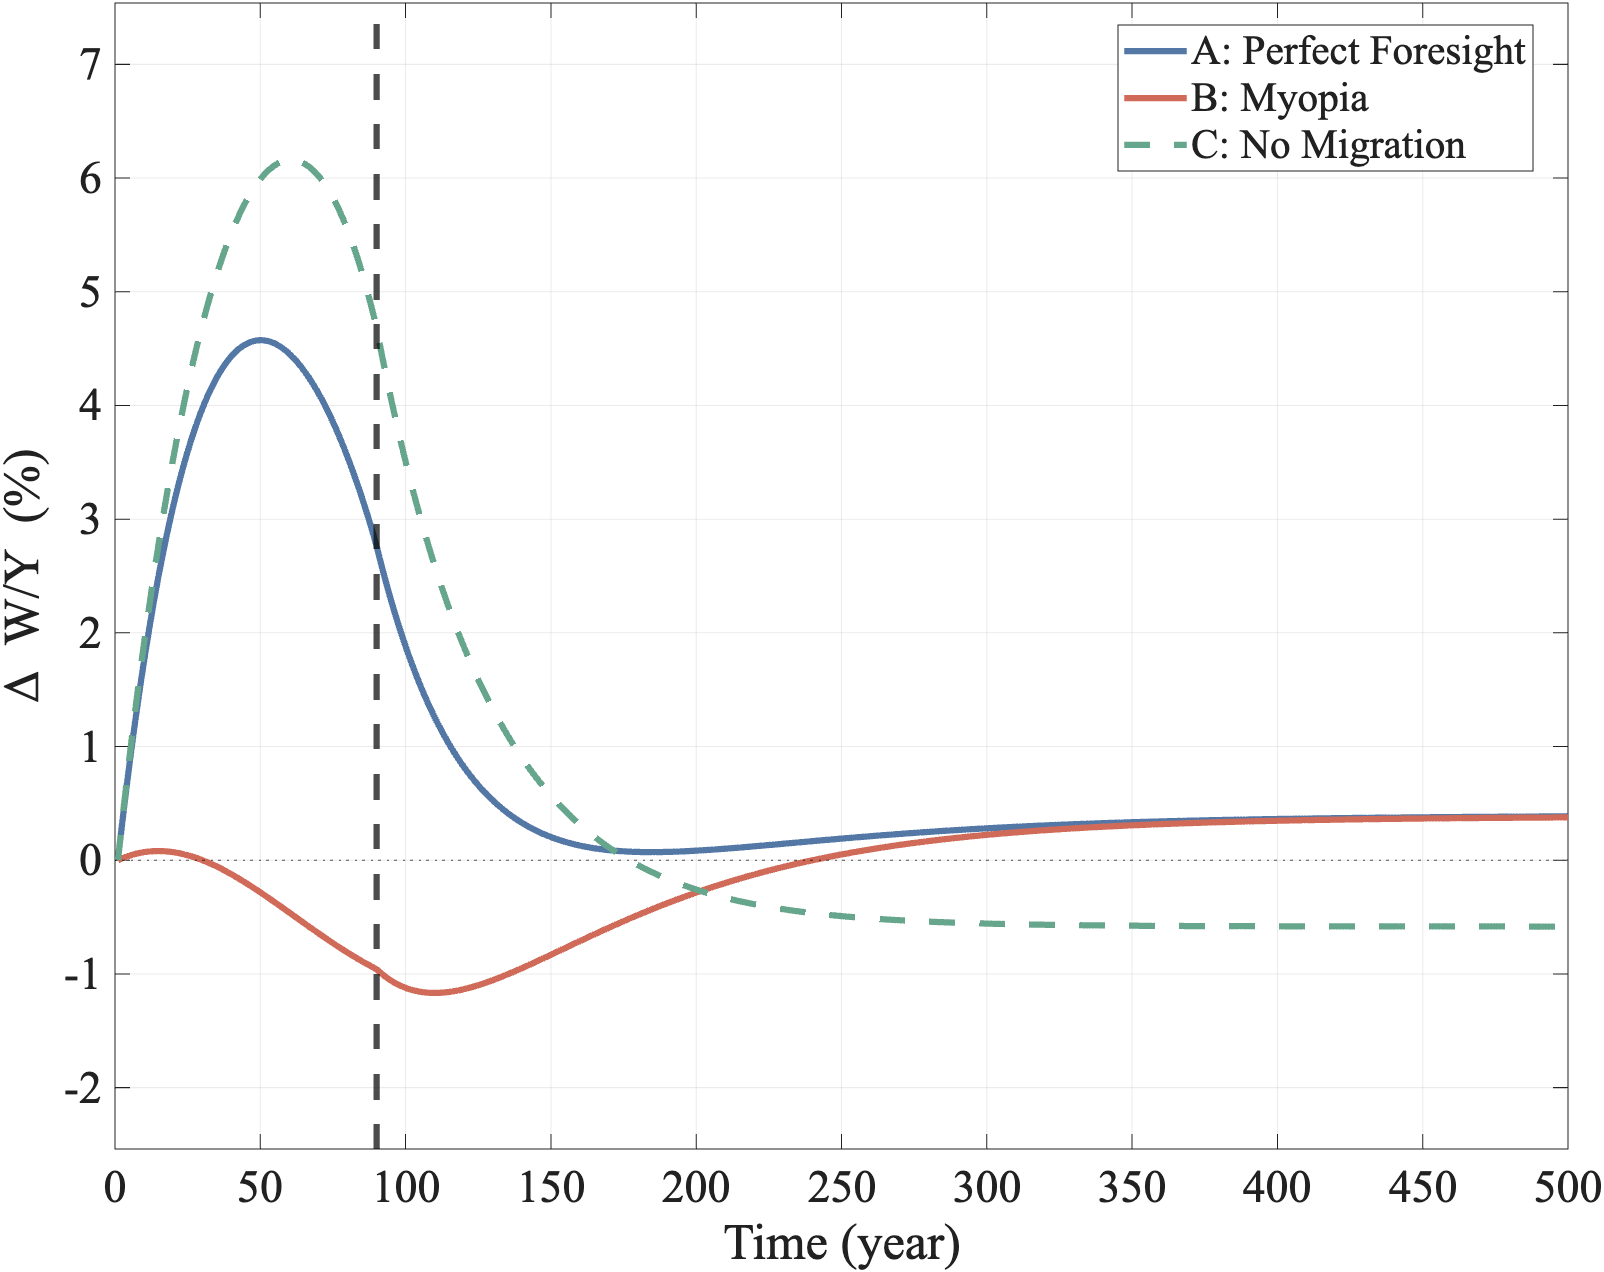
\includegraphics[width=\textwidth]{../Output/big_nu/graph_macro_audit/macro_wy_frictions/macro_wy_frictions_macro_wy_delta_wy_pct.png}
  \end{minipage}
  
  \vspace{2em} 
  \begin{minipage}[t]{0.45\textwidth}
    \centering
    \small{(c) Total Wealth}
    
    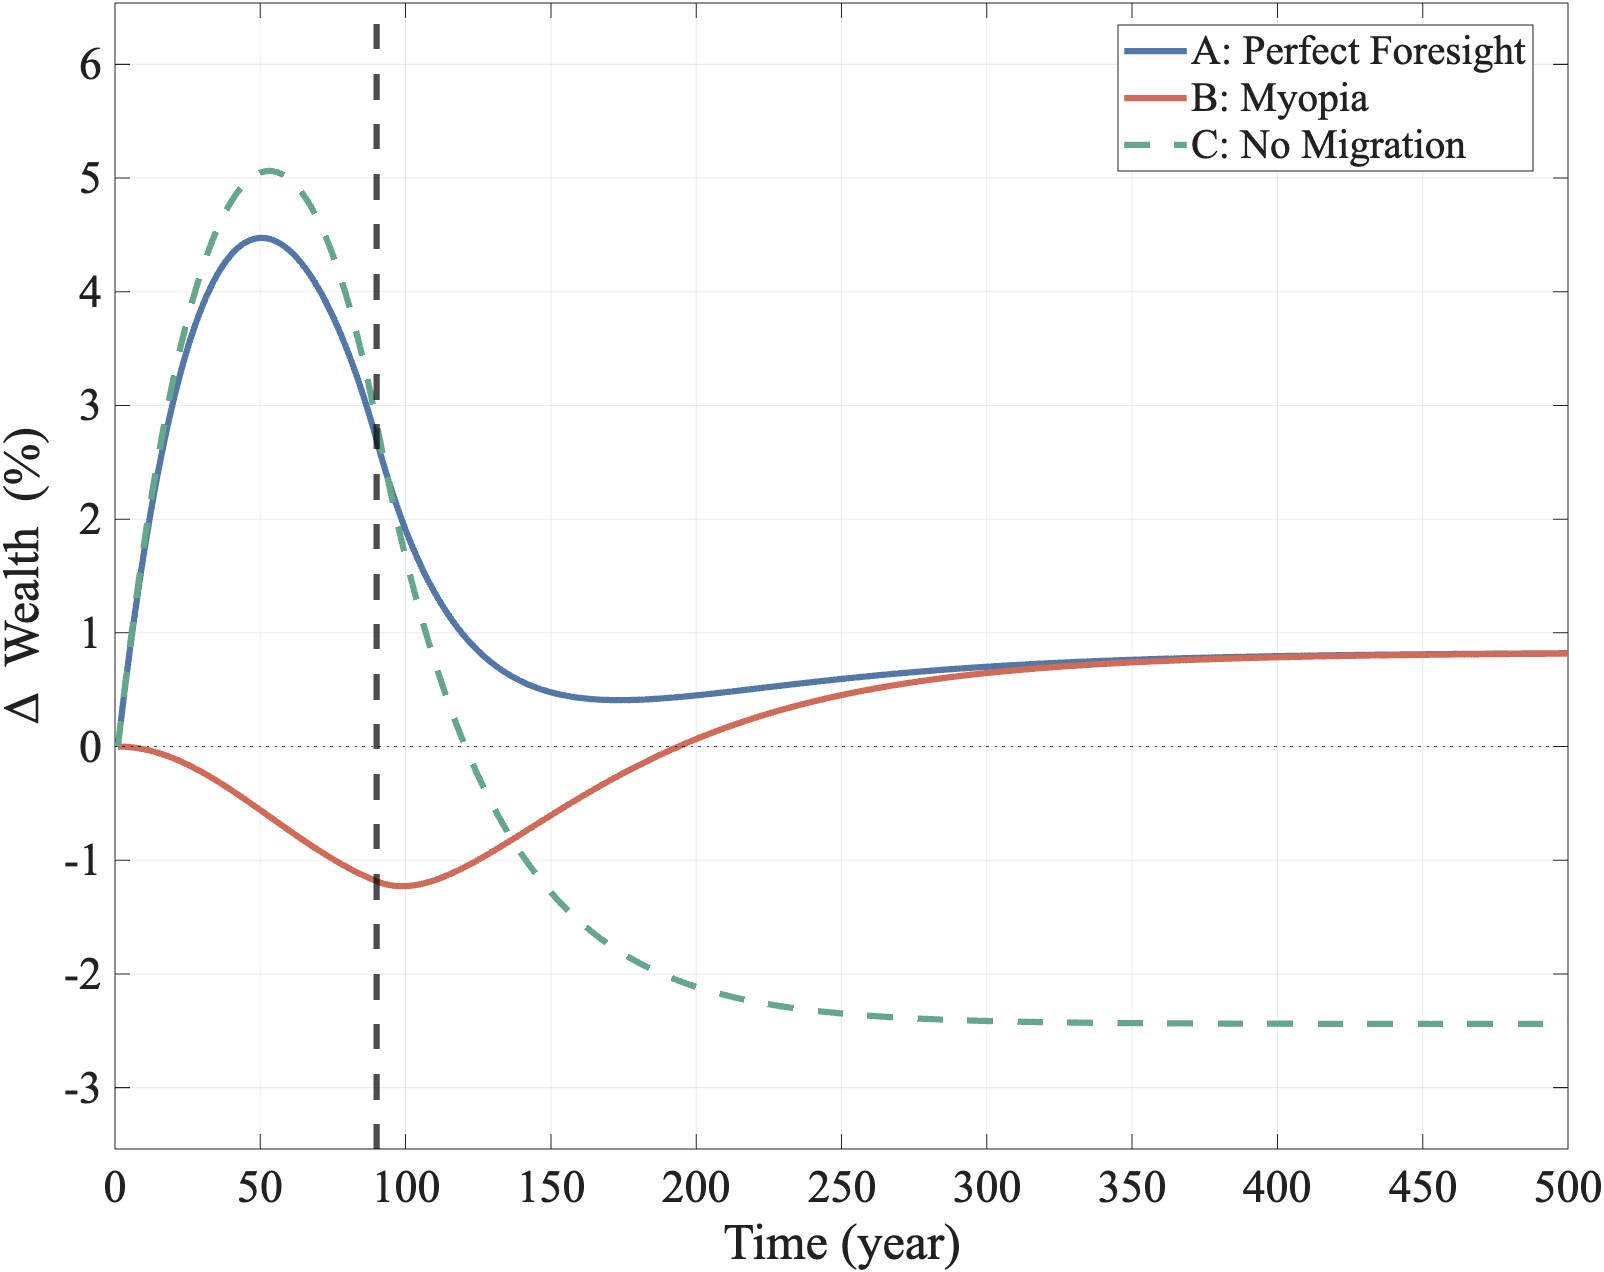
\includegraphics[width=\textwidth]{../Output/big_nu/graph_macro_audit/macro_wealth_frictions/macro_wealth_frictions_macro_wealth_delta_wealth_pct.png}
  \end{minipage}
  \hfill
  \begin{minipage}[t]{0.45\textwidth}
    \centering
    \small{(d) Welfare (CE)}
    
    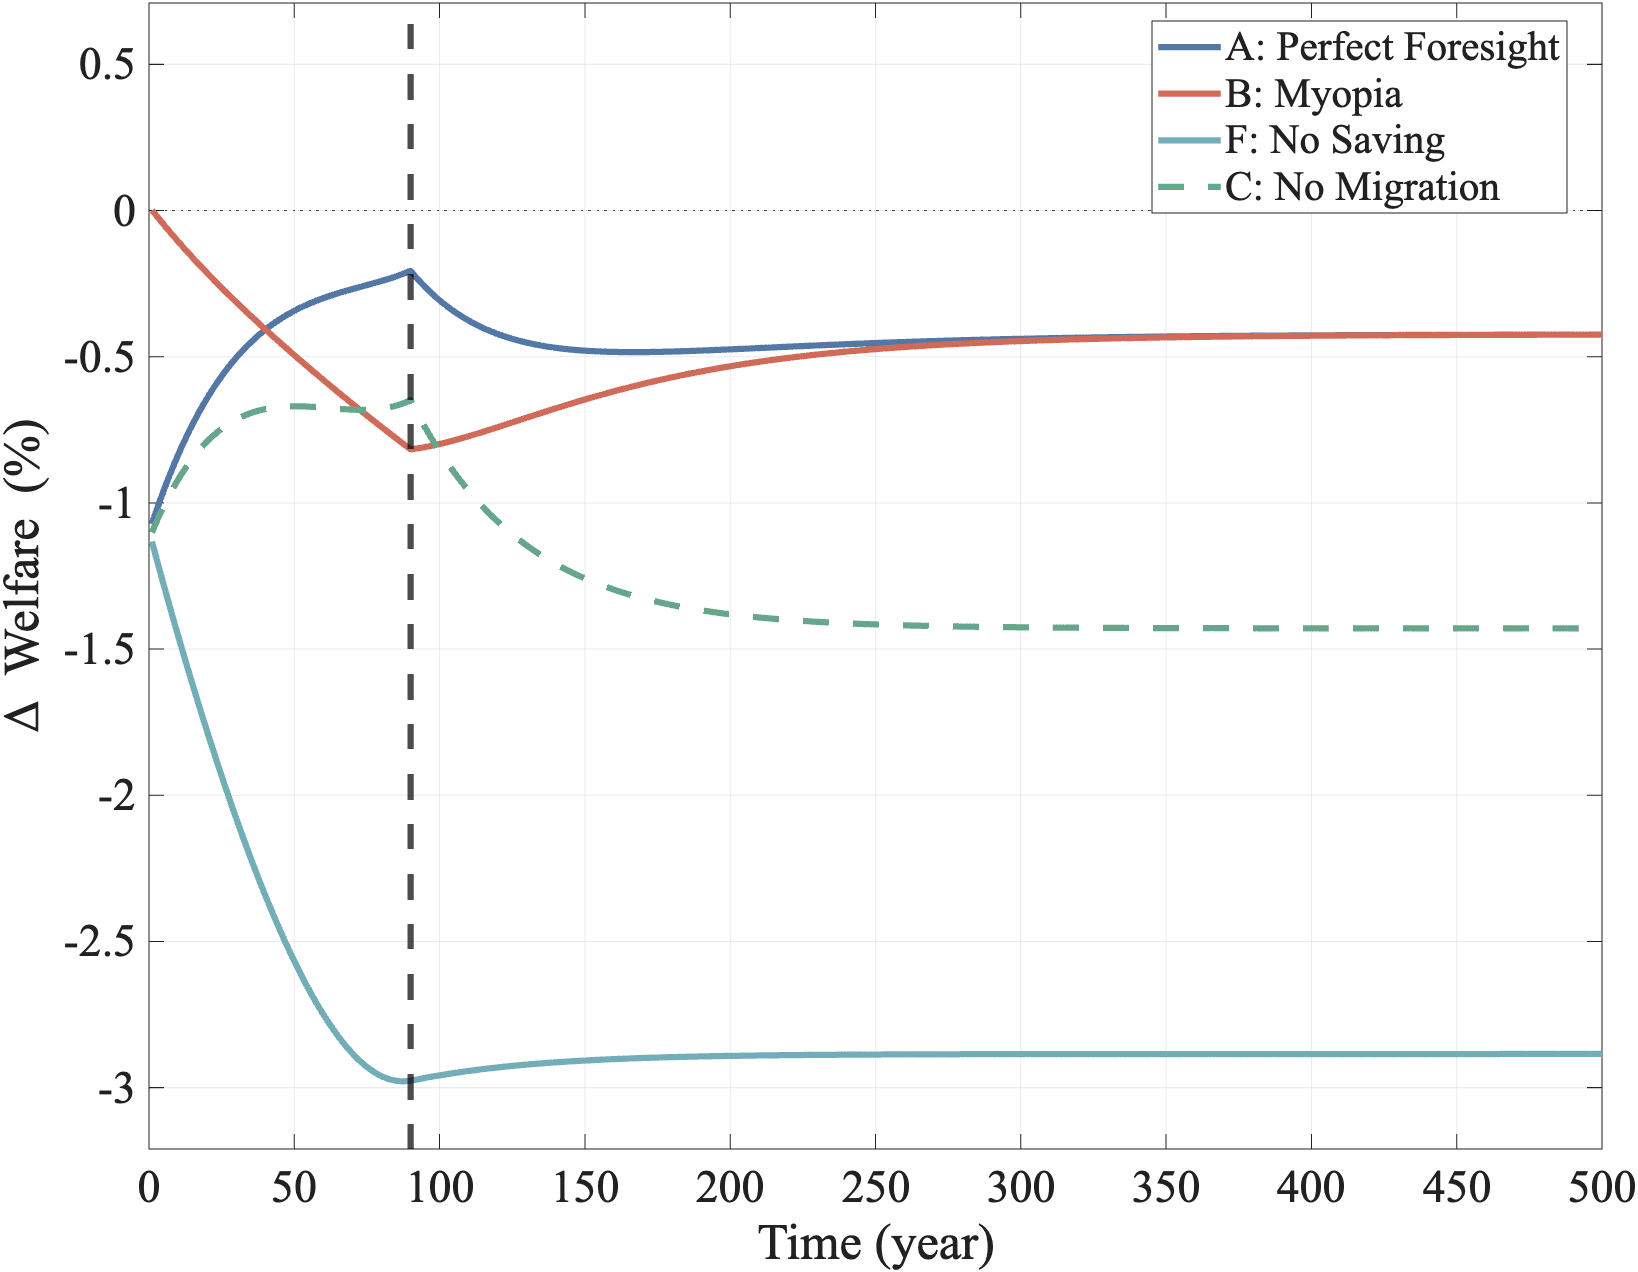
\includegraphics[width=\textwidth]{../Output/big_nu/graph_welfare_audit/welfare_audit_all_scenarios_ce_pct_frictions.png}
  \end{minipage} 
  
  \vspace{0.5em}
  \begin{minipage}{\textwidth}
    \footnotesize{\textbf{Note:} Cross-scenario macro comparison of national aggregate dynamics (for Perfect Foresight, Myopia, No Saving and Autarky scenarios). Panel (a): comparative time series of national total earnings $Y_t = \sum_{\ell,z} \tilde{w}_{\ell,t} (L_{\ell,t} + z \Lambda_t(\ell,z))$. Panels (b) and (c): comparative time series of wealth-to-earnings ratio $(W/Y)_t = W_t / Y_t$ and national wealth mass $W_t = \sum_{\ell,z} \bar{a}_t(\ell,z) \Lambda_t(\ell,z)$. Panel (d): percentage change in aggregate consumption-equivalent (CE) welfare relative to initial aggregate material consumption.} 
  \end{minipage}
  \label{fig:welfare_comp_pc}
\end{figure}

\paragraph{Wealth.} The evolution of wealth and wealth-to-income ratio shows the role of anticipation in generating precautionary savings. The Myopia scenario, without anticipation, is the only one that exhibits a drop in wealth and wealth-to-income ratio before 2100. The No Migration scenario generates a higher peak in the W/Y ratio ($+6\%$ compared to $+4.5\%$ in the baseline), confirming the substitutability between saving and migration during the transition as the absence of migration amplifies the precautionary saving motive. Because of the absence of migration and reallocation of population in higher wage regions at the terminal steady state, the aggregate wealth decreases more than in the baseline (up to -2.5\% for the wealth), showing complementarity between saving and migration at the aggregate level.

\paragraph{Welfare.} At $t = 1$, so right after the climate shock is realised, the welfare loss is the lowest in the Myopia scenario because agents did not anticipate the coming damages and so wrongly expect the rainy days to not come.\footnote{In the context of climate change, it would perhaps be more accurate to talk about the sunny days...} The other scenarios show a welfare loss of 1\% at $t = 1$, which is the result of the anticipation of future damages and results in precautionary saving. Because agents in the Myopia scenario did not anticipate future damages, they do not engage in precautionary saving and thus have more resources to consume in the short run. However, as time progresses and climate damages materialise, the Myopia scenario experiences a larger welfare loss compared to the baseline. At $t = 90$, the Myopia scenario shows a welfare loss of 0.8\%, while the baseline scenario shows a welfare loss of 0.2\% thanks to the accumulation of wealth. The No Migration scenario also exhibits a larger welfare loss at $t = 90$ than the baseline, with a decline of 0.65\%, because of the impossibility to move. According to the model, in the short-run it is therefore better to anticipate climate change without moving than to move without anticipation. For the No Saving scenario, the welfare loss is the largest at $t = 90$ with a decline of 3\%, showing that, in the model, saving is a more important mechanism than migration to smooth climate damages. At the terminal steady state, all scenarios show a welfare loss, with the Myopia and baseline scenario stabilising with a decline of 0.5\% and the No Migration scenario shows a welfare loss of 1.5\% three times larger. The No Saving scenario stabilises at -2.8\%. 

\section{Discussion}
\label{sec:discussion}

\paragraph{CARA Utility Function.}
As stated, the model uses a CARA utility function to ensure that the closed-form solution of the model is tractable and has no borrowing constraint. The CARA utility function has the property that the absolute risk aversion is constant and presents no income effect. Economically, this implicitly assumes complete credit markets where agents can finance moving costs. It makes the model blind to spatial poverty traps, wherein low-wealth households are liquidity-constrained and trapped in geographic areas highly exposed to climate damages. By ignoring these frictions, the framework likely overstates the insurance value of migration for the most vulnerable populations.

\paragraph{Partial Equilibrium and Capital Accumulation.}
The framework is a partial equilibrium endowment economy with no production sector. By fixing the interest rate at $r = 0.03$, the model behaves like a small open economy. In a closed general equilibrium setting, the accumulation of wealth during the 2010-2100 period would drive down the equilibrium interest rate and reduce the return on assets. Furthermore, the absence of endogenous production means the model abstracts from direct climate damages to the physical capital stock, which could depress the marginal product of labour and lower wages (assuming complementarity between capital and labour). Overall, the assumption of an exogenous interest rate and lack of capital accumulation facilitates wealth accumulation, and overstates the efficacy of saving as an adaptation mechanism.

\paragraph{Agglomeration and Dispersion Forces.}
The model does not include agglomeration and dispersion forces. For instance, one could expect that the migration of workers from the South to the North would increase congestion in the North, increasing housing costs and reducing amenities, which would reduce the incentive to migrate. The effect of the population change on wage is unclear as more people in the same location might generate positive externalities with economies of scale or create more congestion on the labour market. Overall, it might overstate the ability of workers to adapt to climate change by moving.

\paragraph{Comparison with the Literature.}
The aggregate welfare loss generated by the baseline model is an order of magnitude smaller than estimates found in other spatial climate studies that focused on the US (e.g., \citet{hsiang_estimating_2017}; \citet{bilal_anticipating_nodate}). This difference is driven by the capacity agents have to endogenously adapt through both spatial mobility and precautionary saving. For instance, \citet{hsiang_estimating_2017} is an econometric analysis that mechanically prevents agents from adjusting. \citet{bilal_anticipating_nodate} restrict the adaptive capacity of labour by modelling mobile hand-to-mouth workers and immobile capitalists that can save. Indeed, in my No Saving counterfactual, which restricts agent behaviour to a framework more closely aligned with standard spatial models, the welfare drop scales to an order of magnitude comparable with the existing literature. While the baseline model may underestimate absolute welfare losses due to the omissions discussed above, it serves as a first step in demonstrating that omitting forward-looking anticipation, saving and migration biases the welfare costs of climate change upward.

\section{Conclusion}

This paper develops a dynamic, quantitative spatial model that integrates saving and migration as joint adaptive mechanisms in response to spatially heterogeneous climate change. While standard spatial models often abstract from saving to preserve tractability, adapting to localised climate shocks requires both spatial reallocation and intertemporal consumption smoothing. By extending the framework of \citet{dvorkin_geography_2025} with a CARA preference structure, this model goes beyond the curse of dimensionality, yielding closed-form decision rules that preserve the heterogeneity of uninsurable income and location preference shocks. Calibrated to the US economy at the state level using damage projections from \citet{hsiang_estimating_2017}, the model provides a tractable set-up to evaluate the transitional dynamics of climate adaptation.

The baseline results underscore the critical role of forward-looking behaviour in mitigating climate damages. Anticipating the deterioration of local fundamentals between 2010 and 2100, workers engage in significant spatial reallocation and accumulate precautionary savings. This dual response smooths the decline in consumption, restricting aggregate welfare losses to a moderate 0.5\%. But aggregate results hide spatial disparities. Climate change reshapes the economic geography of the United States: more impacted regions, notably the Southeast, experience population drop exceeding on average 40\% of their local population and a contraction in their accumulated wealth, while northern and northwestern states absorb these climate migrants and accumulate capital. 

Counterfactual analyses reveal a complex relationship between mobility and wealth, demonstrating that saving and migration both act as substitutes and complements. On the one hand, they can be considered as substitute forms of insurance against local shocks. When mobility is suppressed, workers are forced to rely only on saving, leading to a higher aggregate wealth-to-income ratio to insure against the coming climate change in the 2010-2100 period. Similarly, in an economy of hand-to-mouth agents workers rely more on the migration network to escape climate damages, increasing the inter-state migration rate. In both scenarios, eliminating one adaptive margin amplifies the aggregate welfare losses.

On the other hand, the model shows complementarity between saving and migration, symmetrically across both margins. In the No Saving scenario, precautionary wealth ensures more effective spatial adaptation. As workers bear the full burden of local idiosyncratic income variance which scales with local wages, highly productive Northern states (which would otherwise serve as optimal climate havens) become more risky and workers that move because of climate change go into sub-optimal and lower-variance states. In the No Migration counterfactual, when spatial mobility is suppressed, the spatial discrepancy in wealth accumulation across states is minimised. This occurs because the option to migrate, coupled with uninsurable idiosyncratic location preference shocks, generates a spatial precautionary saving motive: workers in the baseline economy accumulate heterogeneous wealth to insure against the risk of drawing a strong preference for a location with degraded economic fundamentals. Thus, just as savings enable the risk-taking required for optimal mobility, the mobility drives the spatial distribution of wealth.

While this framework provides novel insights into climate adaptation and links between saving and migration, it also points to potential development for future research. First, the tractability of the CARA utility function comes at the cost of suppressing wealth effects on migration. This hides a "climate poverty trap", where the poorest agents are unable to afford the costs of migration and remain in degraded regions. Second, the current endowment economy framework treats wages, housing costs, and the interest rate as exogenous sequences. In reality, the spatial reallocation might trigger general equilibrium price effects. Finally, in the face of climate change, the relationship between saving and migration is likely even more complex than modelled here; climate-change-induced migration might activate inter-regional financial networks, such as remittances and wealth transfers to support relatives remaining in the origin location.


\newpage
\appendix
\numberwithin{equation}{section}
\numberwithin{figure}{section}
\numberwithin{table}{section}
% ---------------------------------------------------------
% APPENDIX
% ---------------------------------------------------------
\section{Proofs and Mathematical Derivations}
\label{app:proofs}
\subsection{Workers' Program Solutions}
The closed-form expressions for individual consumption and saving, and their state- and national-level aggregations, are derived in \citet{dvorkin_geography_2025}. See Appendix B of their paper for the full derivation.

\subsection{Aggregation of Individual Consumption and Saving}
Let $\Lambda_{\ell, t}(z^\prime)$ be the density of workers with shock $z^\prime$ in labour market $\ell$ at the end of period time $t$ and $f_\ell$ the pdf of the $\epsilon$. First, the evolution of the population distribution across locations is given by:
\begin{equation}
\Lambda_{\ell,t}(z^\prime) = (1-\delta) \sum_{j=1}^J \int \Lambda_{j,t-1}(z) \mu_{j\ell,t}(z) f_\ell(z^\prime - \rho z) \mathrm{d}z + \sum_{j=1}^J \mu_{j\ell,t}(0) f_\ell(z^\prime) \left( \delta \int \Lambda_{j,t-1}(z) \mathrm{d}z \right)
\end{equation}
where $\delta$ is the exogenous probability of death. The first term captures surviving workers who relocate from any origin $j$ to destination $\ell$ and draw a new persistent shock $z^\prime$, while the second term accounts for newborns (who start with median productivity $z=0$) choosing location $\ell$ and then drawing their first shock $z^\prime$. 

Given the linearity of the optimal decision rules with respect to cash-on-hand, I can aggregate consumption and wealth at the local level. Under a stationary interest rate $r$, the evolution of average consumption $\bar{c}_{\ell,t}(z^\prime)$ and average asset holdings $\bar{a}_{\ell,t+1}(z^\prime)$ for workers with shock $z^\prime$ in labour market $\ell$ are characterised by:
\begin{align}
\bar{c}_{\ell,t}(z^\prime) &= \sum_{j=1}^J \int \frac{\Lambda_{j,t-1}(z)\mu_{j\ell,t}(z)f_\ell(z^\prime - \rho z)}{\Lambda_{\ell,t}(z^\prime)} (1-\delta) \left( \Xi_{\ell,t}(z^\prime) + \frac{r}{1+r} \tilde{y}_{\ell,t} + \frac{r}{1+r} \bar{a}_{j,t}(z) \right) \mathrm{d}z \nonumber \\
&\quad + \sum_{j=1}^J \frac{\mu_{j\ell,t}(0) f_\ell(z^\prime)}{\Lambda_{\ell,t}(z^\prime)} \left( \Xi_{\ell,t}(z^\prime) + \frac{r}{1+r} \tilde{y}_{\ell,t} + \frac{r}{1+r} \bar{a}^0 \right) \left( \delta \int \Lambda_{j,t-1}(z) \mathrm{d}z \right) 
\end{align}
\begin{align}
\bar{a}_{\ell,t+1}(z^\prime) &= \sum_{j=1}^J \int \frac{\Lambda_{j,t-1}(z)\mu_{j\ell,t}(z)f_\ell(z^\prime - \rho z)}{\Lambda_{\ell,t}(z^\prime)} (1-\delta) \left( \tilde{y}_{\ell,t} + \bar{a}_{j,t}(z) + (1+r)(\tilde{w}_{\ell,t}z^\prime - \Xi_{\ell,t}(z^\prime)) \right) \mathrm{d}z \nonumber \\
&\quad + \sum_{j=1}^J \frac{\mu_{j\ell,t}(0) f_\ell(z^\prime)}{\Lambda_{\ell,t}(z^\prime)} \left( \tilde{y}_{\ell,t} + \bar{a}^0 + (1+r)(\tilde{w}_{\ell,t}z^\prime - \Xi_{\ell,t}(z^\prime)) \right) \left( \delta \int \Lambda_{j,t-1}(z) \mathrm{d}z \right)
\end{align}
where $a^0$ is the exogenous initial wealth endowed to newborns, and $\bar{a}_{j,t}(z)$ is the average asset holding of workers in labour market $j$ with shock $z$ at the end of period $t-1$. Finally, the aggregate level of wealth and consumption per period $t$ are given by:
\begin{align}
  \bar{a}_{t+1} &= \sum_{\ell=1}^J \int \Lambda_{\ell,t}(z^\prime) \bar{a}_{\ell,t+1}(z^\prime) \mathrm{d}z^\prime, \\
  \bar{c}_{t} &= \sum_{\ell=1}^J \int \Lambda_{\ell,t}(z^\prime) \bar{c}_{\ell,t}(z^\prime) \mathrm{d}z^\prime.
\end{align}

\subsection{Derivation of $\Xi$ in the No Saving Scenario}
\label{sec:appendix_no_saving}
In the baseline model, workers possess the ability to save, which yields an optimal consumption path governed by an Euler equation. When this saving margin is suppressed, workers become hand-to-mouth. They consume their full disposable income in every period:
\begin{equation}
c_{\ell,t} = \tilde{y}_{\ell,t} + \tilde{w}_{\ell,t}z^\prime + \tilde{w}_{\ell,t}\eta^\prime
\end{equation}
where $\tilde{y}_{\ell,t} = (1 - D^w_{\ell,t})w_{\ell,t} - q_{\ell,t}(1+ D^q_{\ell,t})$ and $\tilde{w}_{\ell,t} = (1 - D^w_{\ell,t})w_{\ell,t}$.

Let $v_{j,t}(z)$ denote the \textit{ex-ante} expected lifetime utility of a worker in location $j$ with productivity $z$, defined as $v_{j,t}(z) = -\frac{1}{\gamma} e^{-\gamma \Xi_{j,t}(z)}$. The worker's problem is to choose a destination $\ell$ to maximise their utility, subject to moving frictions $e^{\psi_{j\ell}}$ and preference shocks $\varepsilon_\ell$:
\begin{equation}
v_{j,t}(z) = \mathbb{E}_{\varepsilon} \left[ \max_{\ell} \left\{ \varepsilon_\ell e^{\psi_{j\ell}} U_{\ell,t}(z) \right\} \right]
\end{equation}
where $U_{\ell,t}(z)$ is the expected continuation value conditional on selecting destination $\ell$ (prior to the realisation of the new income shocks $z^\prime$ and $\eta^\prime$):
\begin{equation}
U_{\ell,t}(z) = \mathbb{E}_{z^\prime, \eta^\prime | z, \ell} \left[ -\frac{1}{\gamma} e^{-\gamma c_{\ell,t} - \tilde{A}_{\ell,t}} + \beta v_{\ell,t+1}(z^\prime) \right]
\end{equation}

I first evaluate the intra-period expected utility over the normally distributed transitory shock $\eta^\prime \sim \mathcal{N}(0, \sigma_{\eta, \ell}^2)$. Using the moment-generating function of the normal distribution, the expected flow utility simplifies to:
\begin{equation}
\mathbb{E}_{\eta^\prime} \left[ -\frac{1}{\gamma} e^{-\gamma (\tilde{y}_{\ell,t} + \tilde{w}_{\ell,t}z^\prime + \tilde{w}_{\ell,t}\eta^\prime) - \tilde{A}_{\ell,t}} \right] = -\frac{1}{\gamma} \exp\left(F_{\ell,t}(z^\prime)\right)
\end{equation}
where $F_{\ell,t}(z^\prime) \equiv -\gamma \tilde{y}_{\ell,t} - \gamma \tilde{w}_{\ell,t} z^\prime - \tilde{A}_{\ell,t} + \frac{1}{2}(\gamma \tilde{w}_{\ell,t})^2 \sigma_{\eta,\ell}^2$.

Substituting this result and the definition of the \textit{ex-ante} value function $v_{\ell,t+1}(z^\prime)$ back into the conditional continuation value $U_{\ell,t}(z)$, I obtain:
\begin{equation}
U_{\ell,t}(z) = -\frac{1}{\gamma} \mathbb{E}_{z^\prime | z, \ell} \left[ \exp\left(F_{\ell,t}(z^\prime)\right) + \beta \exp\left(-\gamma \Xi_{\ell,t+1}(z^\prime)\right) \right]
\end{equation}

By the properties of the Weibull distribution $\varepsilon_\ell$ (with shape parameter $\nu$ and a normalised scale parameter $\bar{\lambda}$), the expectation of the maximum of these discrete choices yields the closed-form inclusive value:
\begin{equation}
v_{j,t}(z) = -\frac{1}{\gamma} \bar{\lambda} \left[ \sum_{m=1}^J \left( e^{\psi_{jm}} \mathbb{E}_{z^\prime | z, m} \left[ \exp\left(F_{m,t}(z^\prime)\right) + \beta \exp\left(-\gamma \Xi_{m,t+1}(z^\prime)\right) \right] \right)^{-\nu} \right]^{-1/\nu}
\end{equation}

Equating this to our initial definition $v_{j,t}(z) = -\frac{1}{\gamma} e^{-\gamma \Xi_{j,t}(z)}$, taking the natural logarithm, and rearranging the terms allows me to isolate the recursive continuation value $\Xi$:
\begin{equation}
\Xi_{j,t}(z) = -\frac{1}{\gamma} \ln \left( \exp\left(F_{j,t}(z)\right) + \beta \Omega_{j,t}(z) \right)
\end{equation}
where $\Omega_{j,t}(z)$ aggregates the spatial option value across all possible destinations $m$:
\begin{equation}
\Omega_{j,t}(z) = \bar{\lambda} \left[ \frac{1}{J} \sum_{m=1}^J e^{-\nu \psi_{j m}} \left( \mathbb{E}_{z^\prime|z, m} \left[ e^{-\gamma \Xi_{m,t+1}(z^\prime)} \right] \right)^{-\nu} \right]^{-1/\nu}
\end{equation}
This establishes the fixed-point equation required to solve the model backward in the absence of an Euler equation.

\section{Algorithm Description}
\label{app:algorithms}
\subsection{Fixed point for $\Xi$}
Given all estimated and calibrated parameters, the stationary $\Xi^*_\ell(z)$
is the fixed point of operator $\mathcal{T}$ defined by eq.~\eqref{eq:Xi}.
\paragraph{Algorithm}: initialise $\Xi^{(0)} = 0$, iterate until convergence. All numerical expectations are computed using a Rouwenhorst method over the $z$ grid, with a log-sum-exp trick for numerical stability. Warm-starting from the previous $\Xi$ iterate is used inside the calibration exercise and the Myopia scenario to reduce the number of fixed-point iterations per step. 



\subsection{Computation of the Stationary Distribution}

\paragraph{State space and transition matrix.}
The economy has $J \times N_z$ discrete states $k = (\ell, z)$. Under the stationary Markov chain, the transition probability from state $k = (j, z)$ to state $k' = (\ell, z')$ is:
\begin{equation}
  T_{k,k'} = \underbrace{ (1 - \delta) \,\mu_{j\ell}(z) \Pi^\ell_{z, z'}}_{T_{k,k^\prime}^{\text{surv}}}  \;+\;\underbrace{\delta\,\mu_{j\ell}(0)\,\Pi^\ell_{0,z'}}_{T_{k,k^\prime}^{\text{birth}}} ,
\end{equation}
where $\mu_{j\ell}(z)$ is the migration probability from $j$ to $\ell$ conditional on $z$, and $\Pi^\ell$ is the Rouwenhorst transition matrix for the persistent shock in state $\ell$. The full $(J N_z) \times (J N_z)$ matrix $\mathbf{T}$ is then stored.

\paragraph{Population distribution via linear solve.}
New cohorts of mass $\delta$ are born in their \textit{origin} state with a productivity draw at the median grid point $z = 0$, allocated proportionally to the population shares $\{\bar p_\ell\}_{1\le \ell \le J}$. The stationary distribution solves $\boldsymbol{\Lambda} \cdot \mathbf{T} = \boldsymbol{\Lambda}$, where $\boldsymbol{\Lambda}$ is the stationary population mass vector. In MATLAB, this stationary distribution is computed by extracting the left eigenvector associated with the dominant eigenvalue of $1$, using the sparse eigenvalue solver: \verb|[eig_vec, ~] = eigs(T_mat', 1, 'lr')|.

\paragraph{Wealth distribution via linear solve.}
Mean per-capita wealth is recovered from the same system. Define the \textit{income term} for each state $(\ell, z')$ as the savings that accrue to an agent entering that state:
\begin{equation}
  S_\ell(z') = \tilde y_\ell + (1+r)\bigl[\tilde w_\ell z' - \Xi_\ell(z')\bigr].
\end{equation}
The wealth mass vector $\mathbf{A}$ satisfies an analogous Neumann equation:
\begin{equation}
  \mathbf{A} = \boldsymbol{b}_A \cdot (\mathbf{I} - \mathbf{T^{\text{surv}}})^{-1},
  \label{eq:A_inv}
\end{equation}
where $b_A(k) = \Lambda(k) \cdot S(k)$, which can be augmented at the birth states by $\bar p_\ell \cdot \delta \cdot a_0$ to account for newborn endowments (not the case here as I assume no newborn endowments). Mean wealth in state $\ell$ is then $\bar a_\ell = \sum_{z} A(\ell, z) / \sum_{z} \Lambda(\ell, z)$.
\subsection{Computation of the Dynamic Transition}
\label{sec:transition}

Because the original paper compares only two steady states, I introduce a transition-path algorithm. A key property of the CARA specification is that the value-function index $\Xi_\ell(z)$ does not depend on asset holdings~$a$ (cf.\ Section~\ref{sec:model}). This implies that migration probabilities $\mu_{j\ell}(z)$ are also independent of~$a$, which yields a three-stage decomposition: the value function, the population distribution, and the wealth distribution can each be solved sequentially, without joint iteration.
\begin{equation}
  \underbrace{\Xi_T \to \Xi_{T-1} \to \cdots \to \Xi_1}_{\text{Backward: no $\Lambda$, no $a$}}
  \quad\longrightarrow\quad
  \underbrace{\Lambda_1 \to \Lambda_2 \to \cdots \to \Lambda_T}_{\text{Forward: no $a$}}
  \quad\longrightarrow\quad
  \underbrace{\bar a_1 \to \bar a_2 \to \cdots \to \bar a_T}_{\text{Forward: uses both}}
  \label{eq:three_stage}
\end{equation}
Under CRRA or log utility, the value function $V(a,z,\ell)$ would depend on wealth, coupling all three objects and requiring joint value-function iteration on a discretised asset grid at each period.

\paragraph{Parameter paths.}
For each time-varying fundamental $x \in \{w,\, \tilde w,\, \tilde y,\, \sigma^2_\varepsilon,\, \sigma^2_\eta,\, A,\, q\}$, a transition path is constructed over $T_{\text{shock}}$ periods. In the baseline specification, a linear ramp is used:
\begin{equation}
  x_\ell(t) = x_{\ell,0}\!\left(1 - \frac{t}{T_{\text{shock}}}\right) + x_{\ell,T_{\text{shock}}} \cdot \frac{t}{T_{\text{shock}}}, \qquad t = 0,\ldots,T_{\text{shock}}.
  \label{eq:linear_path}
\end{equation}
For $t > T_{\text{shock}}$ the parameters are held constant at their terminal values, padding the horizon to $T_{\text{sim}} = 500$ to allow convergence. Step and exponential ramps are also implemented.

\paragraph{Stage 1: Backward induction on $\Xi$.}
The terminal condition is $\Xi_T = \Xi^*_{SS,T}$, the fixed point of eq.~\eqref{eq:Xi} under the terminal parameters. The algorithm sweeps backward from $t = T{-}1$ to $t = 1$. At each step, the time-varying parameters $(P_t, P_{t+1})$ are read from the path, the location-specific Rouwenhorst matrices $\{\Pi^\ell_{t+1}\}_\ell$ are rebuilt for $t{+}1$, and a single application of eq.~\eqref{eq:Xi} yields $\Xi_t$ from $\Xi_{t+1}$.

\paragraph{Stage 2: Forward simulation of $\Lambda$.}
Starting from $\Lambda_1 = \Lambda^*_{SS,0}$, the population distribution is propagated forward as a matrix product. At each $t$, the migration probability array $\mu_{j\ell}(z)$ is computed from $\Xi_t$ and $B_{1,\ell m,t}$. A  $(JN_z)\times(JN_z)$ transition matrix $\mathbf{T}_t$ is then assembled, with entries:
\begin{equation}
  T_t\bigl((j,z),\,(\ell,z')\bigr)
  = (1-\delta)\,\mu_{j\ell}(z)\,\Pi^\ell_{z,z'}
  \;+\;\delta\,\mu_{j\ell}(z{=}0)\,\Pi^\ell_{0,z'},
  \label{eq:T_sparse}
\end{equation}
where the first term governs surviving agents and the second governs newborns replacing the dead (born at $z=0$, allocated using the same migration probabilities evaluated at the median grid point). The forward update reduces to:
\begin{equation}
  \boldsymbol{\Lambda}_{t+1} = \boldsymbol{\Lambda}_t \cdot \mathbf{T}_t, \qquad
  \boldsymbol{\Lambda}_t \in \mathbb{R}^{1 \times JN_z},
  \label{eq:Lambda_forward}
\end{equation}
followed by renormalisation to unit mass.

\paragraph{Stage 3: Forward computation of wealth.}
Per-capita wealth $\bar a_t(\ell,z)$ is updated forward from the initial condition $\bar a_0 = \bar a^\text{init}$ (this is per-capita wealth at $t = 0$, not the newborn endowment). Because the CARA savings rule (eq.~\ref{eq:apol}) is affine in~$a$, mean wealth evolves linearly. Decomposing the wealth mass arriving at state $(\ell, z')$ into three components:
\begin{equation}
  \underbrace{r\!\sum_{j,z}\Lambda_t(j,z)\,\bar a_t(j,z)\,T^{\mathrm{surv}}_{(j,z),(\ell,z')}}_{\text{survivor wealth transfer}}
  +\;\underbrace{\Lambda_{t+1}(\ell,z')\cdot S_\ell(z')}_{\text{income at destination}}
  +\;\underbrace{\text{NB}_{(\ell,z')}\cdot a_0}_{\text{newborn endowment}},
  \label{eq:a_bar_update}
\end{equation}
where $S_\ell(z') = \tilde y_\ell + (1{+}r)[\tilde w_\ell z' - \Xi_\ell(z')]$ is the net savings increment for an agent arriving at $(\ell,z')$ with zero initial wealth, and $T^{\mathrm{surv}}$ is the survivor-only transition matrix (first term of eq.~\ref{eq:T_sparse}). The survivor wealth transfer is again a single matrix--vector product; per-capita wealth is then recovered by dividing by $\Lambda_{t+1}$.

\paragraph{Aggregate moments.} At each period~$t$, the algorithm computes the different moments of the economy.

\subsection{Estimation of Mobility Costs and Amenities}
\label{sec:mobility}


Dvorkin and Greaney take differences in log-mobility across destinations to identify the composite $[(A_\ell - A_j) - (1-\tilde r)\psi_{j\ell}]$ for all $(j, \ell)$ pairs, \textbf{but \emph{not} amenities and moving costs separately.} To identify amenities and moving costs separately, I implement a two-layer calibration routine structured as nested loops.


\paragraph{Outer loop: \texttt{fsolve} on aggregate moments.}Three scalar parameters $(\psi_{\text{fixed}},\, \psi_{\text{dist}},\, \bar\lambda)$ are jointly identified by solving a system of three moment conditions:
\begin{align}
  \mathcal{M}_1(\theta) &= \frac{\hat m_{\text{mob}} - \bar m_{\text{mob}}}{\bar m_{\text{mob}}} = 0 \label{eq:m1}\\
  \mathcal{M}_2(\theta) &= \frac{\hat d_{\text{avg}} - \bar d_{\text{avg}}}{\bar d_{\text{avg}}} = 0 \label{eq:m2}\\
  \mathcal{M}_3(\theta) &= \frac{\widehat{W/Y} - \overline{W/Y}}{\overline{W/Y}} = 0 \label{eq:m3}
\end{align}
where $\hat m_{\text{mob}}$ is the model aggregate out-migration rate (target: 2.5\%), $\hat d_{\text{avg}}$ is the model average log-distance of moves weighted by flow volumes (target: matched to empirical ACS flows), and $\widehat{W/Y}$ is the model aggregate wealth-to-earnings ratio (target: 4.09). The solver operates on the reparameterised vector $\theta = (\log\psi_{\text{fixed}},\, \log\psi_{\text{dist}},\, \log\bar\lambda)^{\top}$ to enforce positivity. MATLAB's \texttt{fsolve} is used (so this is a root-finding algorithm).

\paragraph{Inner loop: mapping on amenities.} For each evaluation of the outer-loop objective, the $J$ amenity values $\{A_\ell\}$ are recovered by a contraction mapping that inverts the model's predicted population density to match the data. The algorithm proceeds as follows:

\begin{enumerate}[noitemsep]
  \item Define the data population target $\{\tilde p_\ell\}_{1\le \ell \le J}$, where $\tilde p_\ell$ is the empirical population share of state $\ell$.
  \item Initialise $A_\ell^{(0)}$ from the static frictionless approximation:
    \begin{equation}
      A_\ell^{(0)} = \frac{1}{\nu} \log \tilde p_\ell - \hat B_{1,\ell}, \quad
      \hat B_{1,\ell} = \gamma\frac{r}{1+r}\tilde y_\ell - \tfrac{1}{2}(\frac{r}{1+r}\gamma\tilde w_\ell)^2\sigma^2_{\eta,\ell},
      \label{eq:A_init}
    \end{equation}
    centred so that $\sum_\ell A_\ell = 0$.
  \item Iterate the contraction mapping update until convergence:
    \begin{equation}
      A_\ell^{(k+1)} = A_\ell^{(k)} + \frac{1}{\nu}
      \Bigl[\log \tilde p_\ell - \log \hat p_\ell^{(k)}\Bigr], \label{eq:BLP}
    \end{equation}
    where $\hat p_\ell^{(k)} = L_\ell^{(k)}$ and $L_\ell^{(k)} = \sum_{iz} \Lambda(l,iz)$ is the total model population mass in state $\ell$ at iteration $k$, obtained from \texttt{compute\_SS\_moments}. Amenities are re-centred after each update.
\end{enumerate}
Convergence is declared when $\max_\ell |A_\ell^{(k+1)} - A_\ell^{(k)}| < \varepsilon$. 

\subsection{Difference-in-Differences Identification}
To isolate the effect of climate change under alternative migration regimes, the framework implements a Difference-in-Differences (DiD) approach. This method compares two dynamic transition paths that both diverge from the  same initial stationary equilibrium (the 2010 baseline with normal migration frictions).
At $t=1$, a counterfactual migration friction regime $\boldsymbol{\psi}_{\text{variant}}$ is introduced (e.g., a migration ban where $\psi_{j\ell} = 10^8$ for $j \neq \ell$, or scaled moving costs). The economy is then simulated forward under two parallel arms:
\begin{enumerate}[noitemsep]
    \item The Control Arm ($X_t^{\text{Ctrl}}$): The new migration friction is imposed, but the climate parameters remain constant at their 2010 baseline values (no climate change).
    \item The Treatment Arm ($X_t^{\text{Treat}}$): The new migration friction is imposed, and the economy is simultaneously exposed to the projected climate change shocks transitioning from 2010 to 2100.
\end{enumerate}
The Difference-in-Differences isolator for any aggregate or state-level outcome $X_t$ is defined as:
\begin{equation}
    \Delta^{\text{DiD}} X_t = X_t^{\text{Treat}}\left(P_{\text{climate}}, \boldsymbol{\psi}_{\text{variant}}\right) - X_t^{\text{Ctrl}}\left(P_{\text{no\_climate}}, \boldsymbol{\psi}_{\text{variant}}\right)
\end{equation}
Because both the treatment and control arms start from the identical steady state and are subjected to the new migration policy at $t=1$, the pre-shock difference is zero. Therefore, the difference at any time $t$ provides the effect of the climate shock under the counterfactual mobility regime. This isolates the climate impact from the transitional dynamics induced by the change in migration frictions.
For welfare evaluation, the aggregate Certainty Equivalent (CE) loss from climate change at time $t$ under the counterfactual regime is:
\begin{equation}
    \Delta^{\text{DiD}} \text{CE}_t^{\text{agg}} = \text{CE}_t^{\text{agg, Treat}} - \text{CE}_t^{\text{agg, Ctrl}}
\end{equation}
By comparing this isolated welfare loss against the baseline scenario with free migration, I can quantify the insurance value of spatial mobility.

\subsection{Algorithm for the Spatial Decomposition}
\label{sec:algorithm_spatial_decomp}

The objective of the spatial decomposition is to disentangle aggregate wealth changes between the baseline steady state ($t=0$) and the counterfactual steady state ($t=1$) into behavioural and compositional margins. The decomposition aims at isolating behavioural responses (e.g., precautionary savings) from the demographic effects caused by climate-induced migration, while respecting the mathematical identity of lifetime wealth accumulation. 

Let $s_{\ell,t}(z)$ denote the local savings flow in state $\ell$ with productivity shock $z$ at time $t$, and let $\tilde{T}_t$ denote the time-reversed Markov transition matrix over the state space. Total accumulated wealth is given by the recursive sum $a_t = (I - \tilde{T}_t)^{-1} s_t$.

\paragraph{Step 1: Compute Autarky Counterfactuals.} 
To prevent spatial option values from contaminating the deterministic income channel, I construct first an autarky counterfactual. By imposing infinite moving costs ($\psi_{\ell m} \to \infty$ for $\ell \neq m$), I compute the autarky continuation value $\Xi_{\text{aut}, t}$ and extract the baseline autarky transition matrix $\tilde{T}_{\text{aut}, 0}$ (which is a block-diagonal matrix as people cannot move).

\paragraph{Step 2: Decompose the Saving Rule.}
The change in the local savings flow, $\Delta s_{\ell}(z) = s_{\ell,1}(z) - s_{\ell,0}(z)$, is separated into three fundamental channels:
\begin{align}
    \Delta s_{\text{Dam}} &= \frac{\Delta \tilde{y}_\ell}{1+r} + \Delta \tilde{w}_\ell z - \Delta \mathbb{E}_{z^\prime|z}[\Xi_{\ell,\text{aut}}(z^\prime)] \\
    \Delta s_{\text{Risk}} &= \frac{1}{\gamma} \Delta \log \mathbb{E}_{z^\prime|z}[e^{-\gamma \Xi_{\ell}(z^\prime)}] + \Delta \mathbb{E}_{z^\prime|z}[\Xi_{\ell}(z^\prime)] + \Delta \text{Risk}_{\text{Trans}} \\
    \Delta s_{\text{Spat}} &= \Delta s_{\ell}(z) - \Delta s_{\text{Dam}} - \Delta s_{\text{Risk}}
\end{align}
These discrete-time components correspond to the mechanisms isolated in Equation \eqref{eq:intensive_margin_decomposition}. $\Delta s_{\text{Dam}}$ serves as the numerical analogue to the Damage Dampening effect ($\Delta s_{\text{Dam}} \approx - z \rho^s (1-\rho) w \Delta^{SS} D^w_\ell$). $\Delta s_{\text{Risk}}$ isolates the shift in precautionary savings due to altered income variance ($\Delta s_{\text{Risk}} \propto \Delta \sigma_{C, \ell}^2$). $\Delta s_{\text{Spat}}$ absorbs the residual value of the spatial option.

\paragraph{Step 3: Accumulate Flows into Wealth Stocks.}
Because climate change simultaneously alters both savings behaviour ($\Delta s$) and the spatial network ($\Delta \tilde{T}$), standard shift-share identities face cross-term interactions. To isolate the behavioural effect and align with a \textit{no-migration} counterfactual, the saving rule margins are accumulated using the baseline autarky network $\tilde{T}_{\text{aut}, 0}$:
\begin{align}
    a_{\text{Dam}} &= (I - \tilde{T}_{\text{aut}, 0})^{-1} \Delta s_{\text{Dam}} \\
    a_{\text{Risk}} &= (I - \tilde{T}_{\text{aut}, 0})^{-1} \Delta s_{\text{Risk}}
\end{align}
By breaking the spatial network, we prevent a dilution  effect, where an influx of migrants changes the state-average wealth of receiving states. The \textit{Spatial Option} channel is then formulated to absorb the network premium (the difference between accumulating wealth over the baseline spatial network versus autarky), preserving the sum identity:
\begin{equation}
    a_{\text{Spat}} = (I - \tilde{T}_0)^{-1} \Delta s - a_{\text{Dam}} - a_{\text{Risk}}
\end{equation}

\paragraph{Step 4: Isolate Spatial Transition and Compositional Sorting.}
The effect of agents changing their migration trajectories (the shift in the transition matrix) is captured by the \textit{Spatial Transition} channel. To maintain the accounting identity $a_1 - a_0 = a_{\text{Dam}} + a_{\text{Risk}} + a_{\text{Spat}} + a_{\text{Trans}}$, this channel absorbs the behavioural cross-term by evaluating the network change at the \textit{new} savings behaviour $s_1$:
\begin{equation}
    a_{\text{Trans}} = a_1 - (I - \tilde{T}_0)^{-1} s_1
\end{equation}
The micro-responses are aggregated to the state level $\ell$. To complete the shift-share decomposition on the state-level averages $\bar{a}_{\ell,t}$, I weight the former margins by the baseline demographic shares $\pi_0$, and assign the remaining spatial variation to \textit{Compositional Sorting} of the productivity distribution:
\begin{align}
    \bar{a}_{\ell,1} - \bar{a}_{\ell,0} &= \sum_{z} \pi_0(z|\ell) \left[ a_{\text{Dam}} + a_{\text{Risk}} + a_{\text{Spat}} + a_{\text{Trans}} \right] + \sum_{z} \left( \pi_1(z|\ell) - \pi_0(z|\ell) \right) a_{\ell,1}(z)
\end{align}

\section{Additional Results and Scenarios}
\label{app:additional}
\subsection{High Mig. Cost}

% 1. Dynamic Moments Diff (4 in a line)
\begin{figure}[H]
  \centering
  \caption{Dynamic Moments Diff (High Mig. Cost (DiD))}
  \begin{minipage}[t]{0.4\textwidth}
    \centering
    \small{(a) Earnings Diff}
    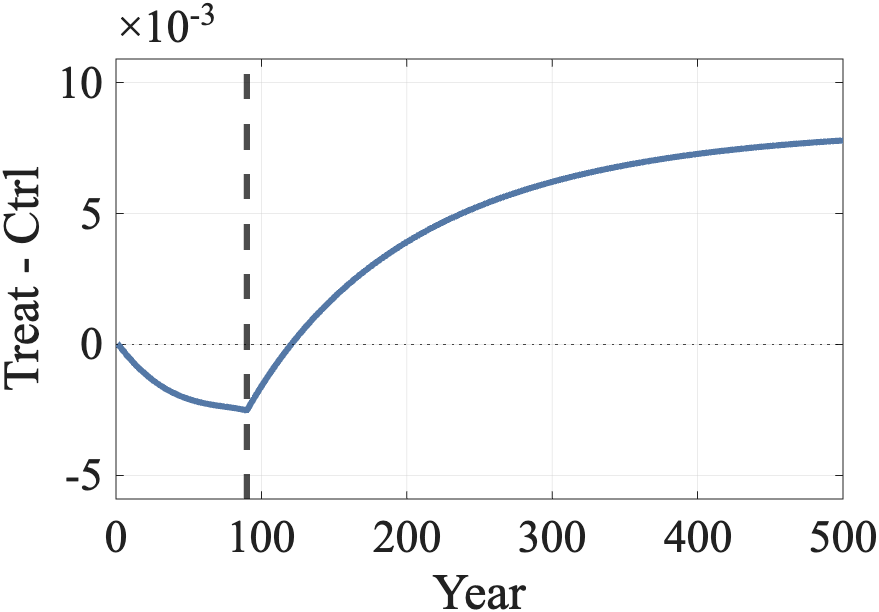
\includegraphics[width=\textwidth]{../Output/big_nu/graph_small_migration_did/did_dynamic_moments_diff_earnings.png}
  \end{minipage}\hfill
  \begin{minipage}[t]{0.4\textwidth}
    \centering
    \small{(b) Migration Diff}
    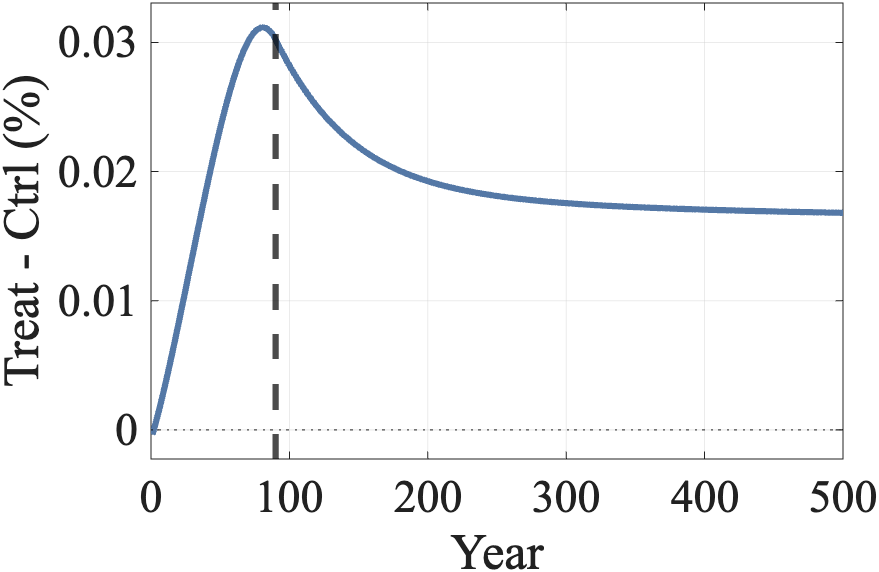
\includegraphics[width=\textwidth]{../Output/big_nu/graph_small_migration_did/did_dynamic_moments_diff_migration.png}
  \end{minipage} \\[2ex]
  \begin{minipage}[t]{0.4\textwidth}
    \centering
    \small{(c) Wealth Diff}
    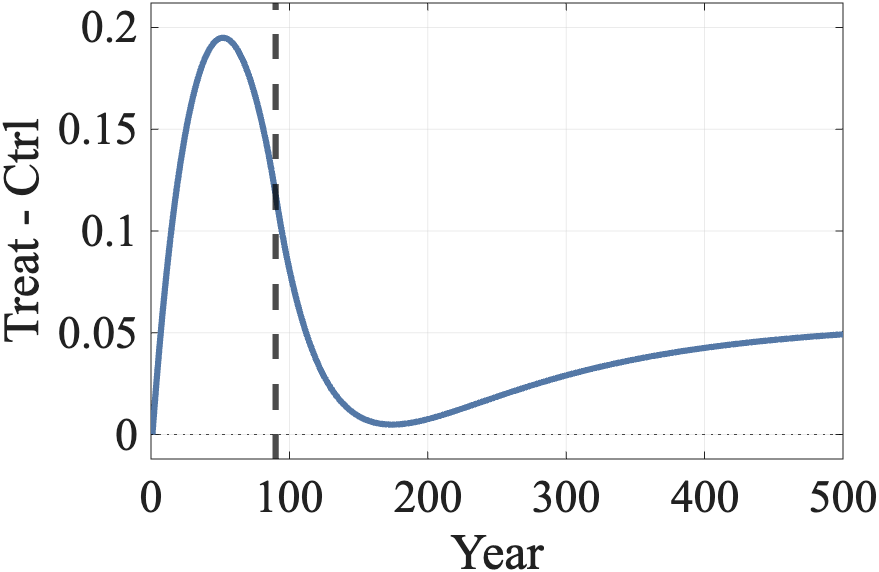
\includegraphics[width=\textwidth]{../Output/big_nu/graph_small_migration_did/did_dynamic_moments_diff_wealth.png}
  \end{minipage}\hfill
  \begin{minipage}[t]{0.4\textwidth}
    \centering
    \small{(d) W/Y Diff}
    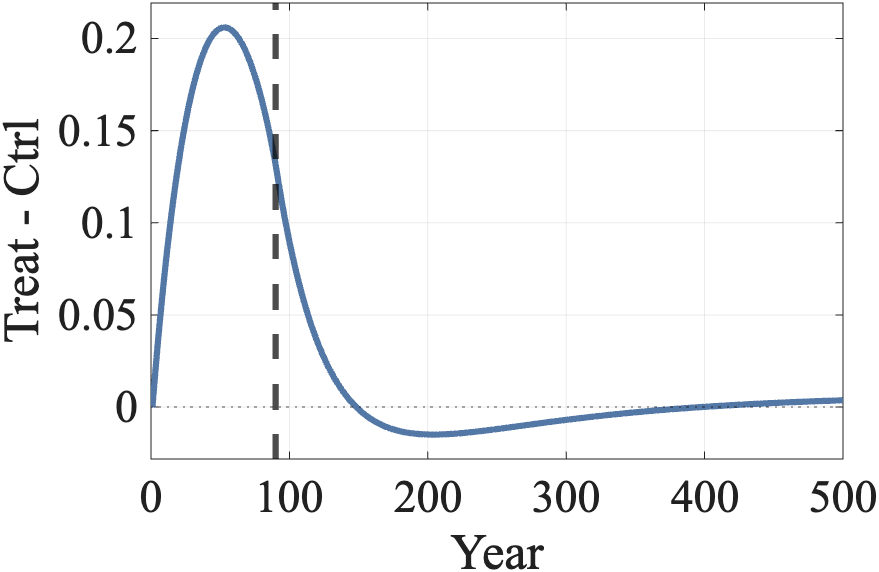
\includegraphics[width=\textwidth]{../Output/big_nu/graph_small_migration_did/did_dynamic_moments_diff_wy.png}
  \end{minipage}
  \begin{minipage}{\textwidth}
  \vspace{0.5em}
  \footnotesize{\textbf{Note:} Difference-in-Differences (DiD) macro dynamic trajectories under High Mig. Cost / 10\% moving cost increase counterfactual. Metrics measure climate treatment differential $\Delta^{\text{DiD}} X_t = X_t^{\text{Treat}} - X_t^{\text{Ctrl}}$. Panel (a): annual earnings treatment diff $\Delta^{\text{DiD}} Y_t$. Panel (b): gross migration rate treatment diff $\Delta^{\text{DiD}} m_t$. Panel (c): total wealth treatment diff $\Delta^{\text{DiD}} W_t$. Panel (d): wealth-to-earnings ratio treatment diff $\Delta^{\text{DiD}} (W/Y)_t$.} \end{minipage}
  \label{fig:high_mig_1}
\end{figure}

% 2. Transition Maps (2x2)
\begin{figure}[H]
  \centering
  \caption{Transition Maps (High Mig. Cost)}
  \begin{minipage}[t]{0.4\textwidth}
    \centering
    \small{(a) $\Delta$ Mean Welfare (CE)}
    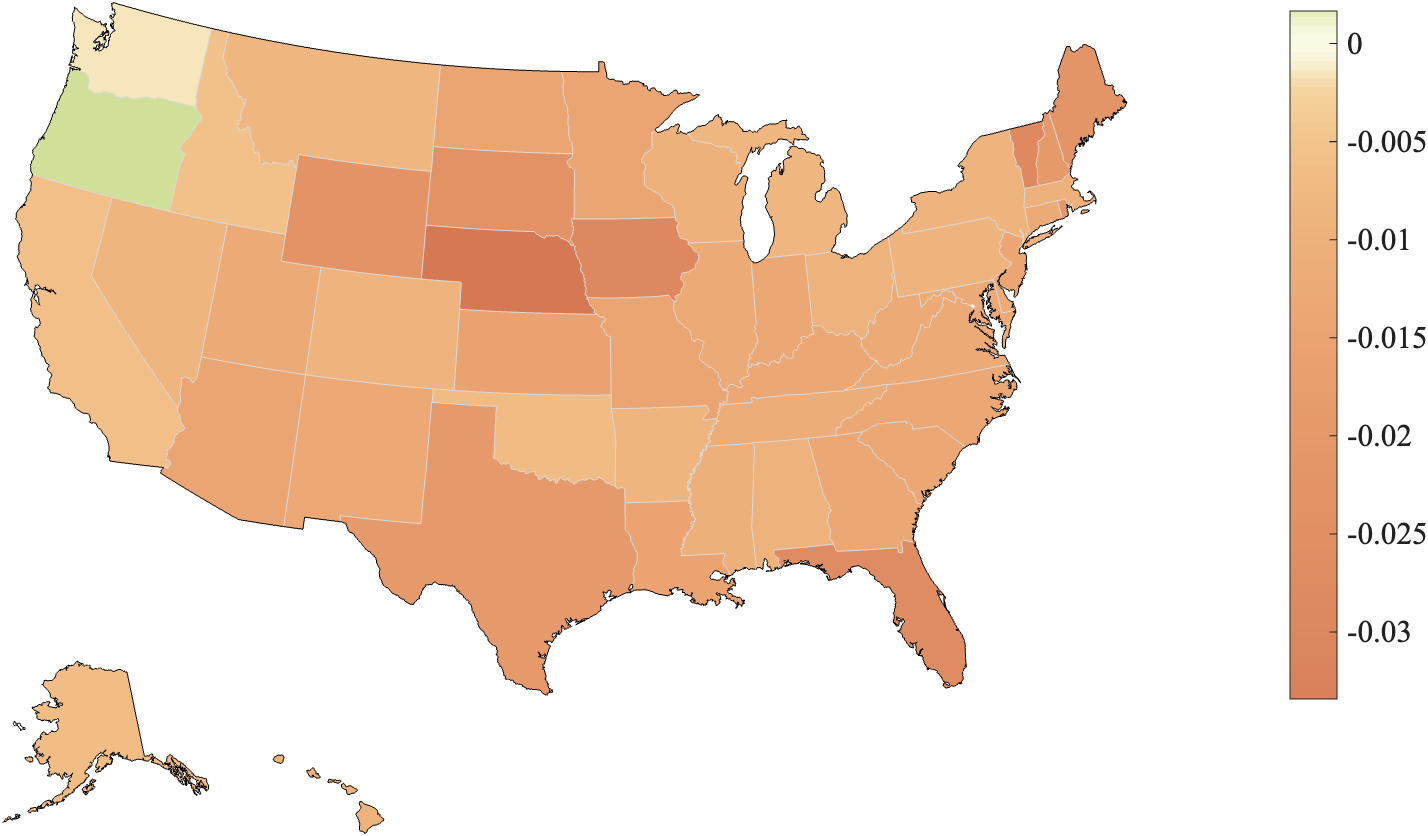
\includegraphics[width=\textwidth]{../Output/big_nu/graph_small_migration_did/transition_maps/transition_maps_delta_mean_welfare_ce.png}
  \end{minipage}\hfill
  \begin{minipage}[t]{0.4\textwidth}
    \centering
    \small{(b) $\Delta$ W/Y Ratio in level}
    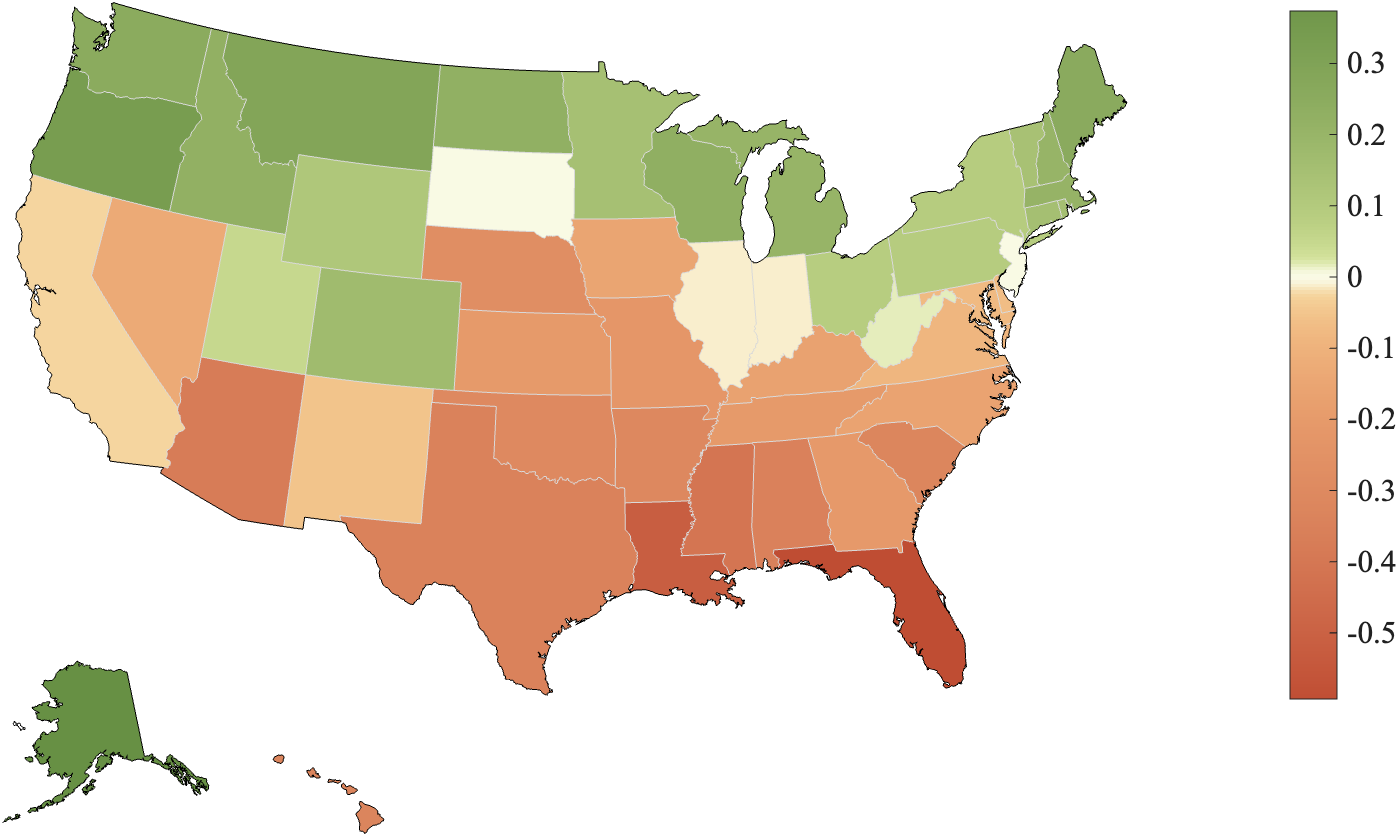
\includegraphics[width=\textwidth]{../Output/big_nu/graph_small_migration_did/transition_maps/transition_maps_wealth_income_ratio_changes.png}
  \end{minipage}
  \vspace{1em}
  \begin{minipage}[t]{0.4\textwidth}
    \centering
    \small{(c) $\Delta$ Local Population (\%)}
    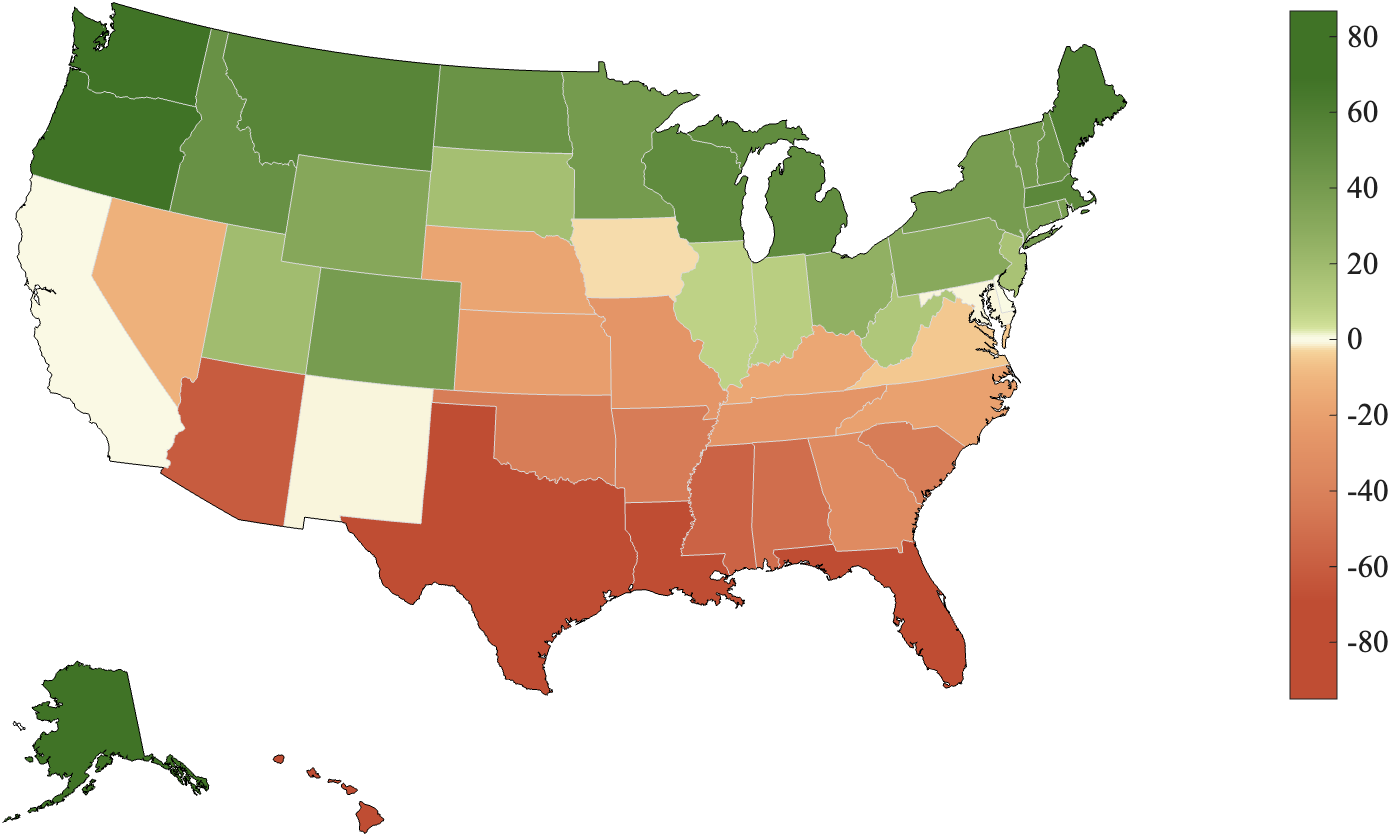
\includegraphics[width=\textwidth]{../Output/big_nu/graph_small_migration_did/transition_maps/transition_maps_local_pop_changes_pct.png}
  \end{minipage}\hfill
  \begin{minipage}[t]{0.4\textwidth}
    \centering
    \small{(d) $\Delta$ Mean Wealth (\%)}
    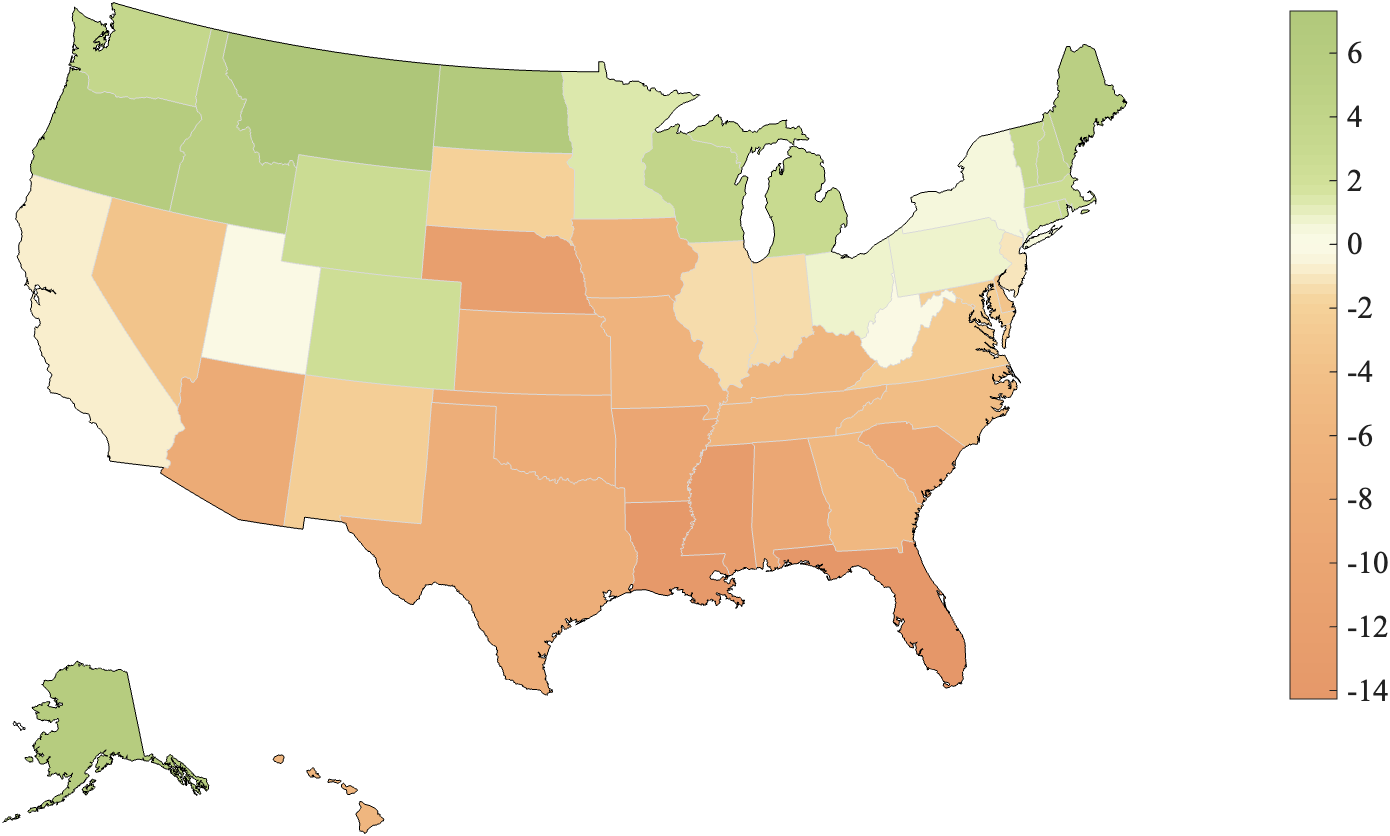
\includegraphics[width=\textwidth]{../Output/big_nu/graph_small_migration_did/transition_maps/transition_maps_pop_changes_pp.png}
  \end{minipage}
  \begin{minipage}{\textwidth} 
  \vspace{0.5em}
  \footnotesize{\textbf{Note:} Spatial maps comparing the terminal steady state under 2100 climate parameters ($SS_\text{term}$) to the initial 2010 baseline steady state ($SS_\text{init}$) under Scenario High Mig. Cost / 10\% moving cost increase. Panel (a): change in mean Certainty Equivalent welfare $\Delta \text{CE}_\ell = \overline{\text{CE}}_{\ell, \text{term}} - \overline{\text{CE}}_{\ell, \text{init}}$. Panel (b): change in state wealth-to-earnings ratio $\Delta (W/Y)_\ell = (W/Y)_{\ell, \text{term}} - (W/Y)_{\ell, \text{init}}$. Panel (c): relative population percentage change $\Delta L_\ell\% = 100 \times (L_{\ell, \text{term}} - L_{\ell, \text{init}})/L_{\ell, \text{init}}$. Panel (d): percentage change in state mean per-capita wealth $\Delta \bar{a}_\ell\%$.}
  \end{minipage}
  \label{fig:high_mig_2}
\end{figure}

% 3. Welfare Inequality Maps only (1x2)
\begin{figure}[H]
  \centering
  \caption{Inequality Maps (High Mig. Cost)}
  \begin{minipage}[t]{0.4\textwidth}
    \centering
    \small{(a) $\Delta$ Welfare Inequality (Std Dev \%)}
    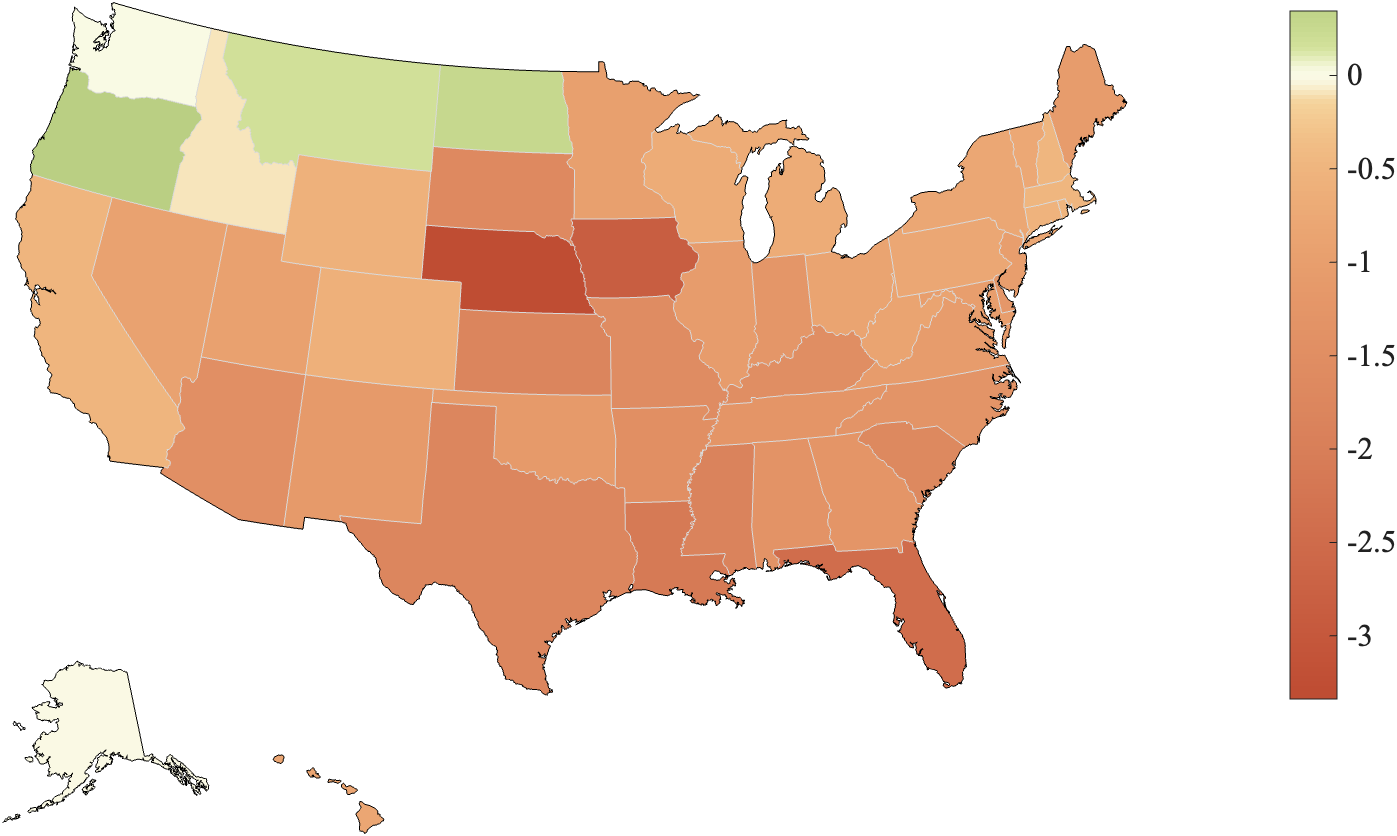
\includegraphics[width=\textwidth]{../Output/big_nu/graph_small_migration_did/welfare_wealth_inequality_maps/welfare_wealth_inequality_maps_welfare_inequality.png}
  \end{minipage}\hfill
  \begin{minipage}[t]{0.4\textwidth}
    \centering
    \small{(b) $\Delta$ Wealth Inequality (Std Dev \%)}
    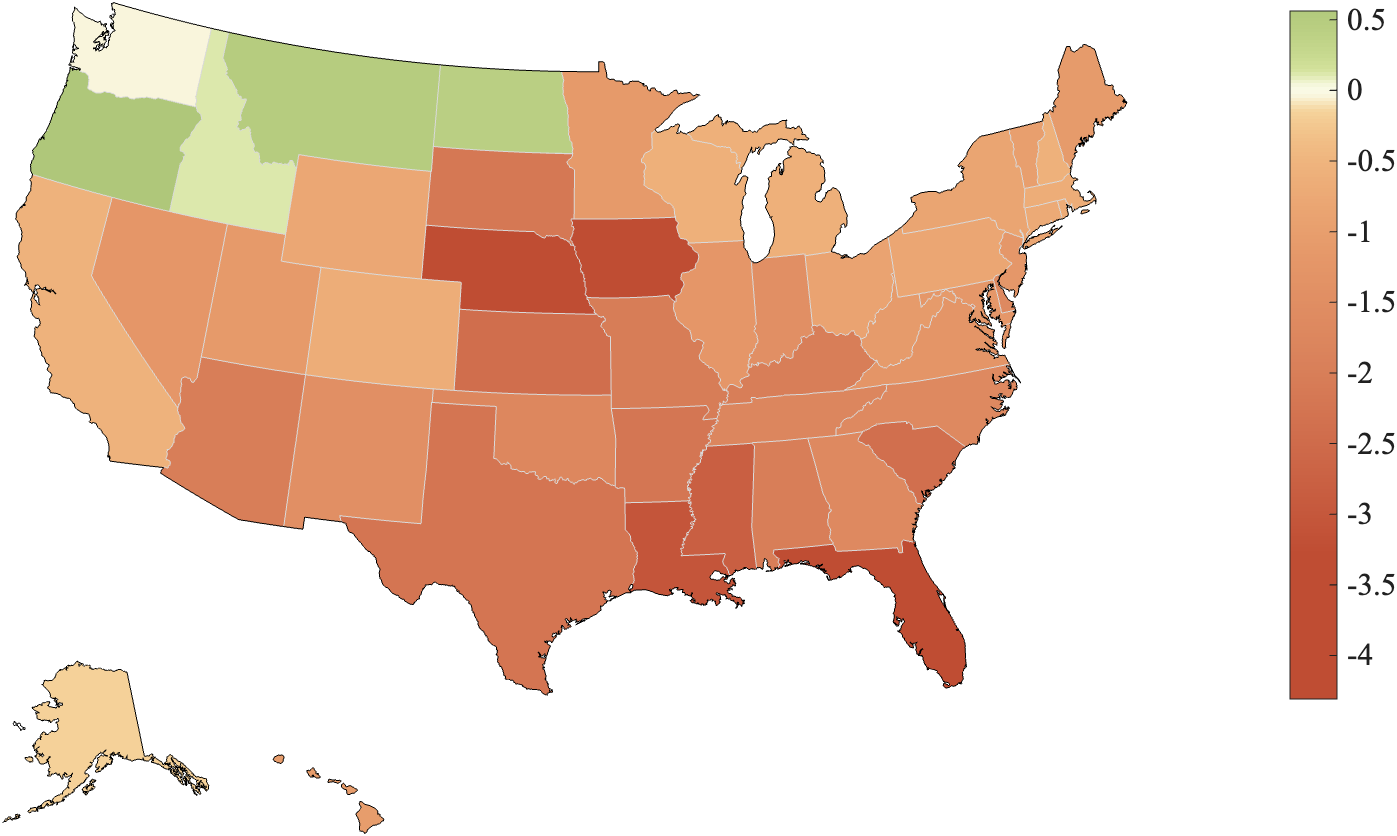
\includegraphics[width=\textwidth]{../Output/big_nu/graph_small_migration_did/welfare_wealth_inequality_maps/welfare_wealth_inequality_maps_wealth_inequality.png}
  \end{minipage}
  \begin{minipage}{\textwidth}
  \vspace{0.5em}
  \footnotesize{\textbf{Note:} Spatial inequality maps under High Mig. Cost / 10\% moving cost increase. Panel (a): percentage change in the within-state welfare standard deviation $\text{Var}_z(\text{CE}_\ell(z)) = \frac{1}{L_\ell} \sum_z \Lambda(\ell,z) [\text{CE}_\ell(z) - \overline{\text{CE}}_\ell]^2$ between the two steady states. Panel (b): percentage change in the within-state wealth standard deviation $\text{Var}_z(\bar{a}_\ell(z)) = \frac{1}{L_\ell} \sum_z \Lambda(\ell,z) [\bar{a}_\ell(z) - \bar{a}_\ell]^2$ between the two steady states.} \end{minipage}
  \label{fig:high_mig_3}
\end{figure}

\begin{figure}[H]
  \centering
    \caption{Wealth Decomposition (Low Mig. Cost)}
  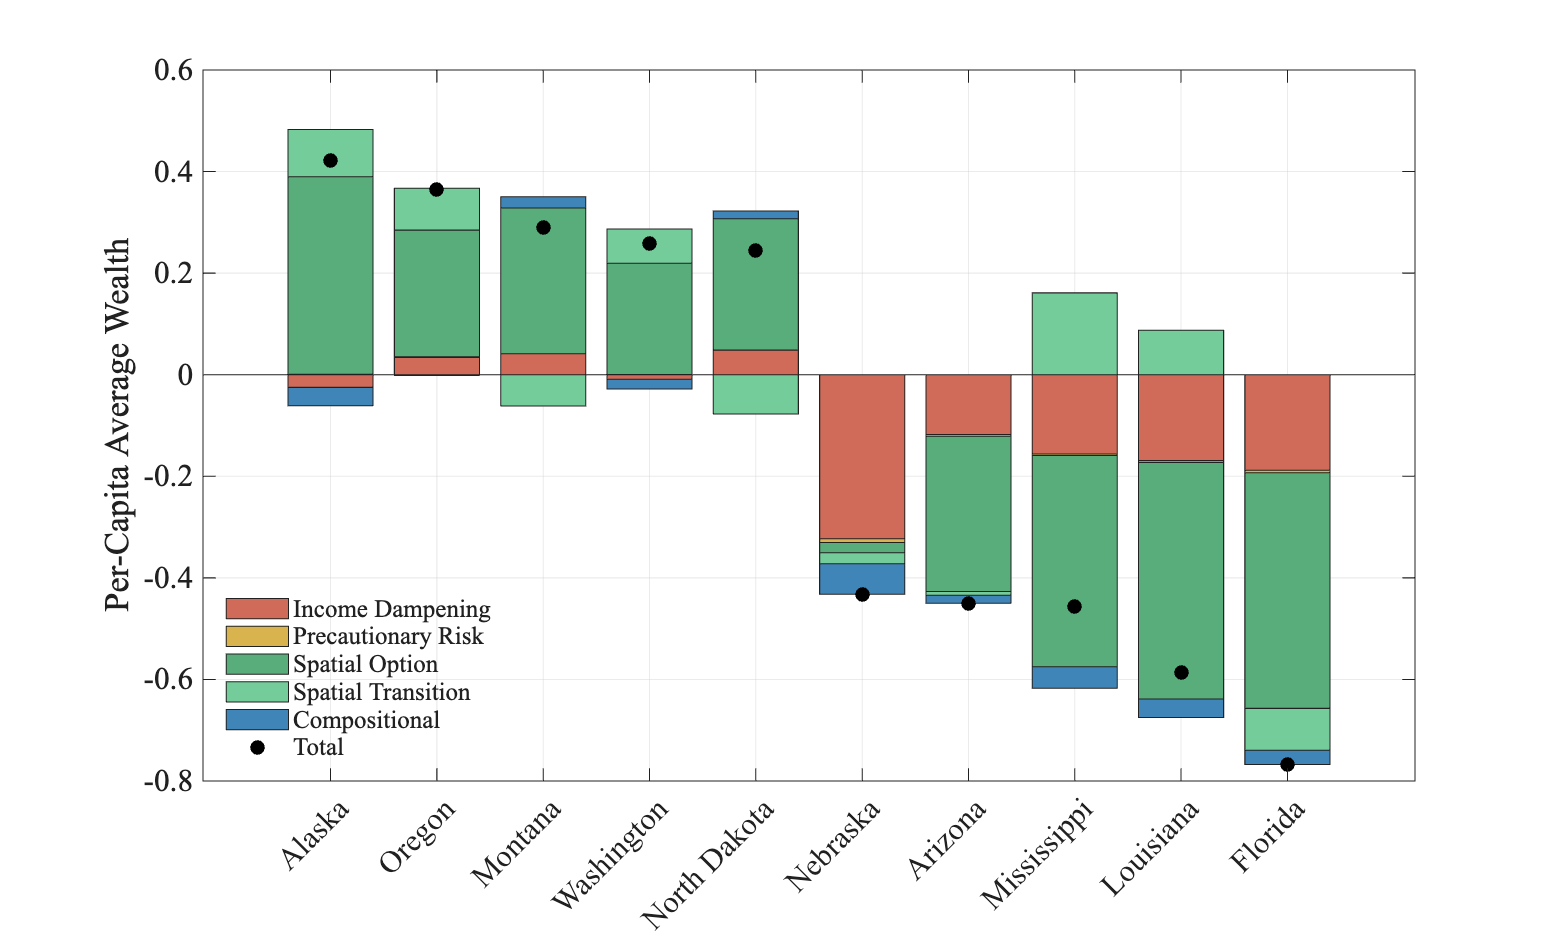
\includegraphics[width=\textwidth]{../Output/big_nu/graph_small_migration_did/exact_percapita_decomposition_bar_did_small_migration_Treat_vs_Ctrl.png}
  \begin{minipage}{\textwidth}
  \vspace{0.5em}
  \footnotesize{\textbf{Note:} Structural shift-share decomposition of the state-level per-capita wealth change $\Delta \bar{a}_\ell = \bar{a}_{\ell, \text{term}} - \bar{a}_{\ell, \text{init}}$ under Low Mig. Cost into five margins: (1) Income Dampening: savings adjustments to income changes evaluated at the baseline autarky network; (2) Precautionary Risk: shifts in savings due to altered income variance evaluated at autarky; (3) Spatial + Amenity: network premium from accumulating wealth over the baseline spatial network versus autarky; (4) Spatial Transition: change in the migration network evaluated at the new savings behaviour; (5) Compositional: changes in local productivity shares.}
  \end{minipage}
  \label{fig:low_mig_4}
\end{figure}

\subsection{Low Mig. Cost}

% 1. Dynamic Moments Diff (4 in a line)
\begin{figure}[H]
  \centering
  \caption{Dynamic Moments Diff (Low Mig. Cost (DiD))}
  \begin{minipage}[t]{0.4\textwidth}
    \centering
    \small{(a) Earnings Diff}
    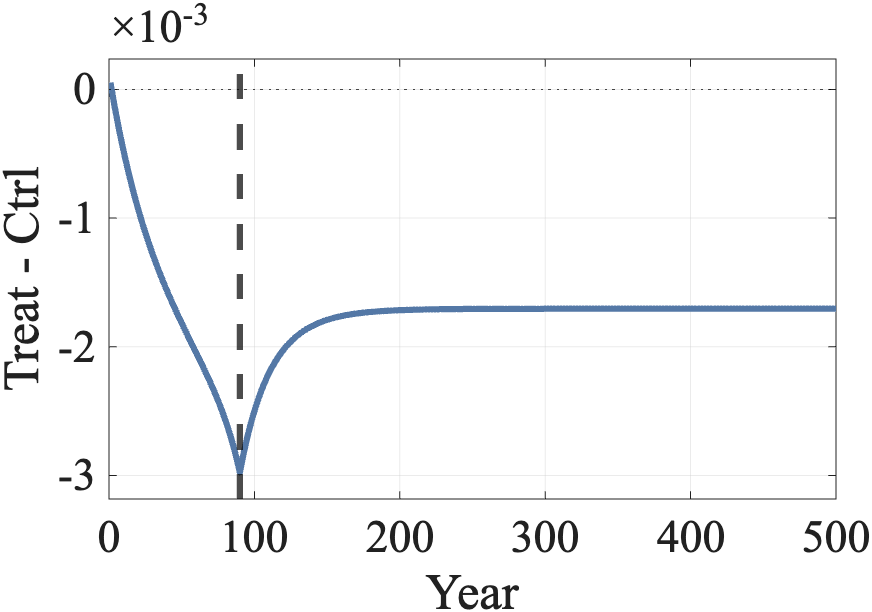
\includegraphics[width=\textwidth]{../Output/big_nu/graph_big_migration_did/did_dynamic_moments_diff_earnings.png}
  \end{minipage}\hfill
  \begin{minipage}[t]{0.4\textwidth}
    \centering
    \small{(b) Migration Diff}
    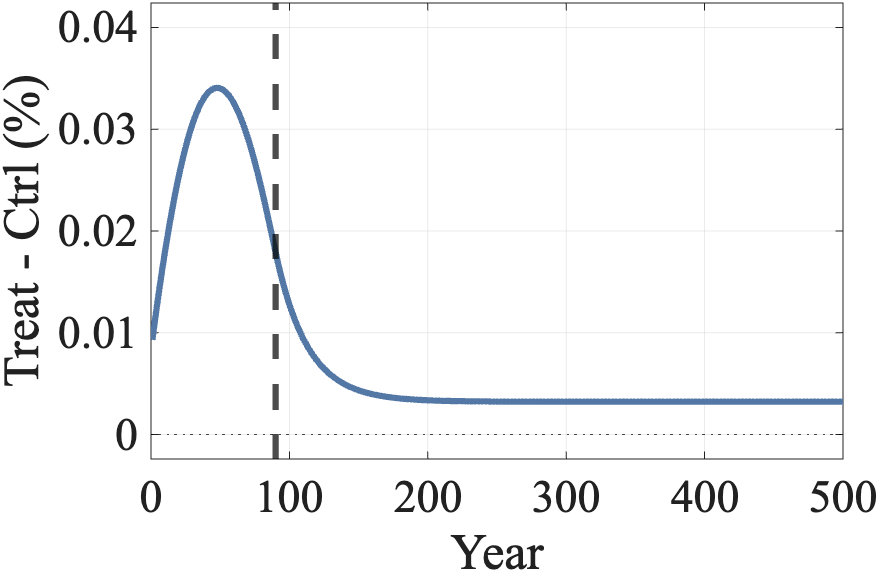
\includegraphics[width=\textwidth]{../Output/big_nu/graph_big_migration_did/did_dynamic_moments_diff_migration.png}
  \end{minipage} \\[2ex]
  \begin{minipage}[t]{0.4\textwidth}
    \centering
    \small{(c) Wealth Diff}
    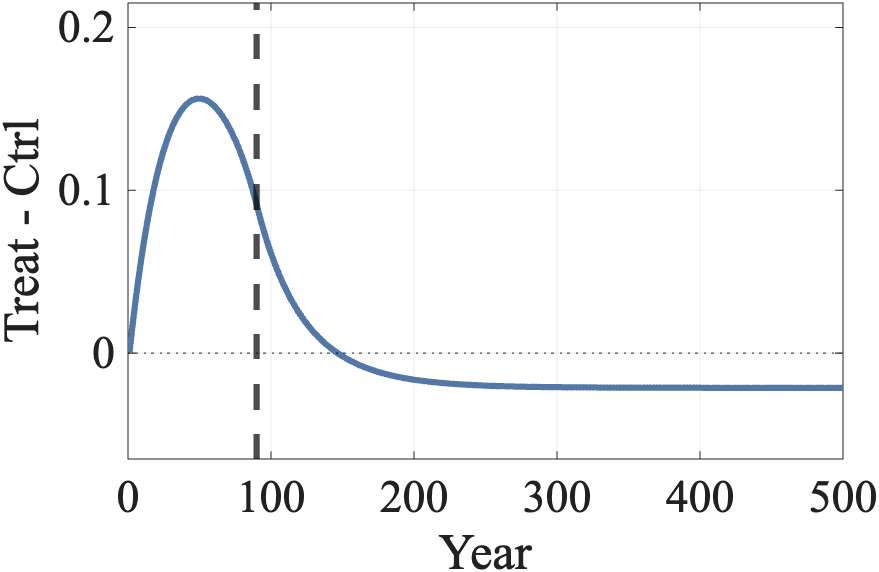
\includegraphics[width=\textwidth]{../Output/big_nu/graph_big_migration_did/did_dynamic_moments_diff_wealth.png}
  \end{minipage}\hfill
  \begin{minipage}[t]{0.4\textwidth}
    \centering
    \small{(d) W/Y Diff}
    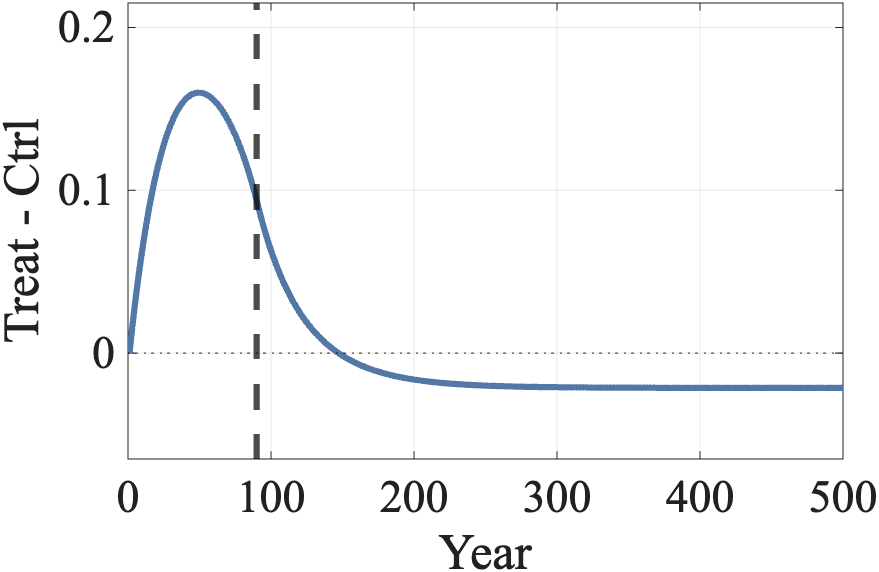
\includegraphics[width=\textwidth]{../Output/big_nu/graph_big_migration_did/did_dynamic_moments_diff_wy.png}
  \end{minipage}
  \begin{minipage}{\textwidth}
  \vspace{0.5em}
  \footnotesize{\textbf{Note:} Difference-in-Differences (DiD) macro dynamic trajectories under Low Mig. Cost / 10\% moving cost reduction counterfactual. Metrics measure climate treatment differential $\Delta^{\text{DiD}} X_t = X_t^{\text{Treat}} - X_t^{\text{Ctrl}}$. Panel (a): annual earnings treatment diff $\Delta^{\text{DiD}} Y_t$. Panel (b): gross migration rate treatment diff $\Delta^{\text{DiD}} m_t$. Panel (c): total wealth treatment diff $\Delta^{\text{DiD}} W_t$. Panel (d): wealth-to-earnings ratio treatment diff $\Delta^{\text{DiD}} (W/Y)_t$.} \end{minipage}
  \label{fig:low_mig_1}
\end{figure}

% 2. Transition Maps (2x2)
\begin{figure}[H]
  \centering
  \caption{Transition Maps (Low Mig. Cost)}
  \begin{minipage}[t]{0.4\textwidth}
    \centering
    \small{(a) $\Delta$ Mean Welfare (CE)}
    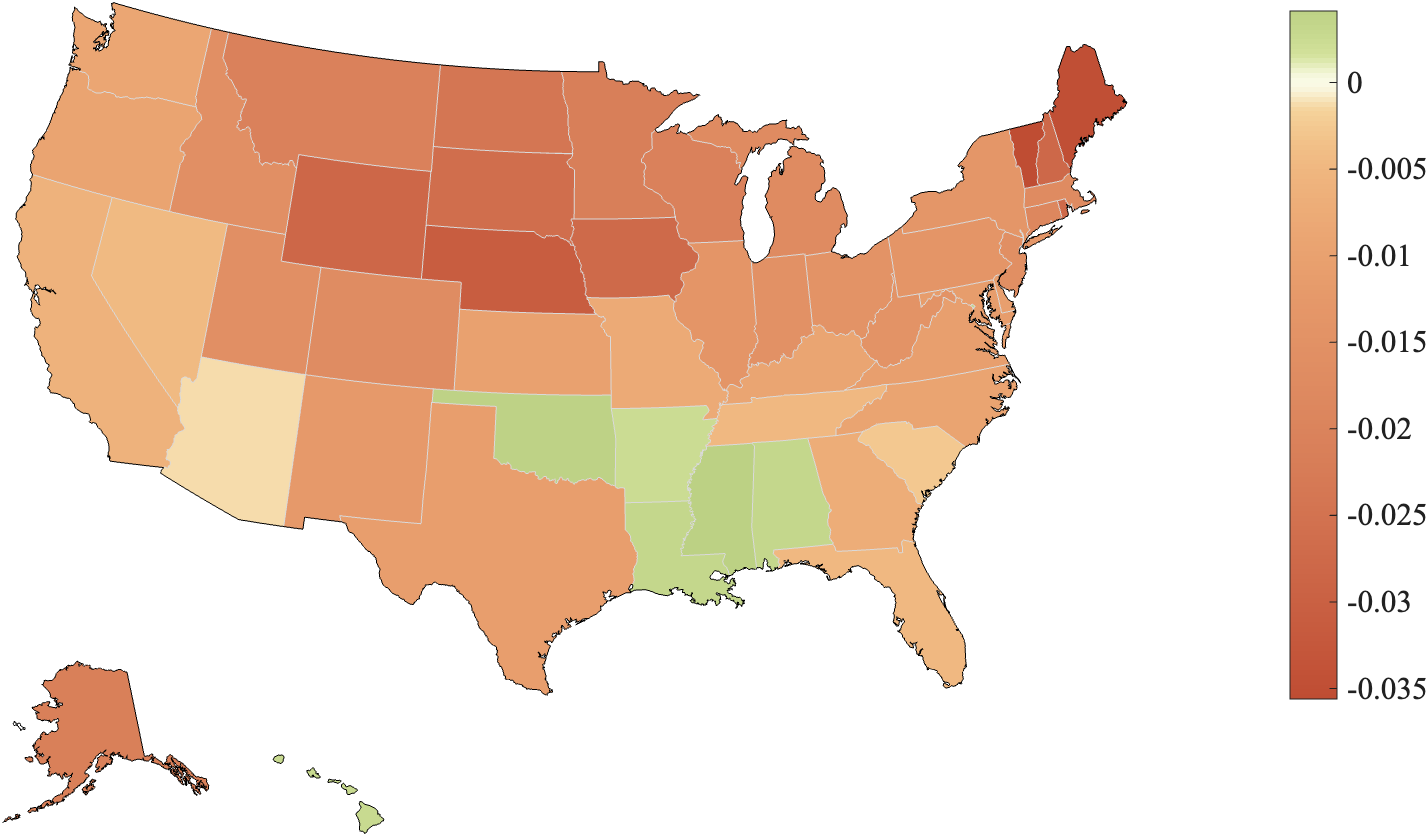
\includegraphics[width=\textwidth]{../Output/big_nu/graph_big_migration_did/transition_maps/transition_maps_delta_mean_welfare_ce.png}
  \end{minipage}\hfill
  \begin{minipage}[t]{0.4\textwidth}
    \centering
    \small{(b) $\Delta$ W/Y Ratio in level}
    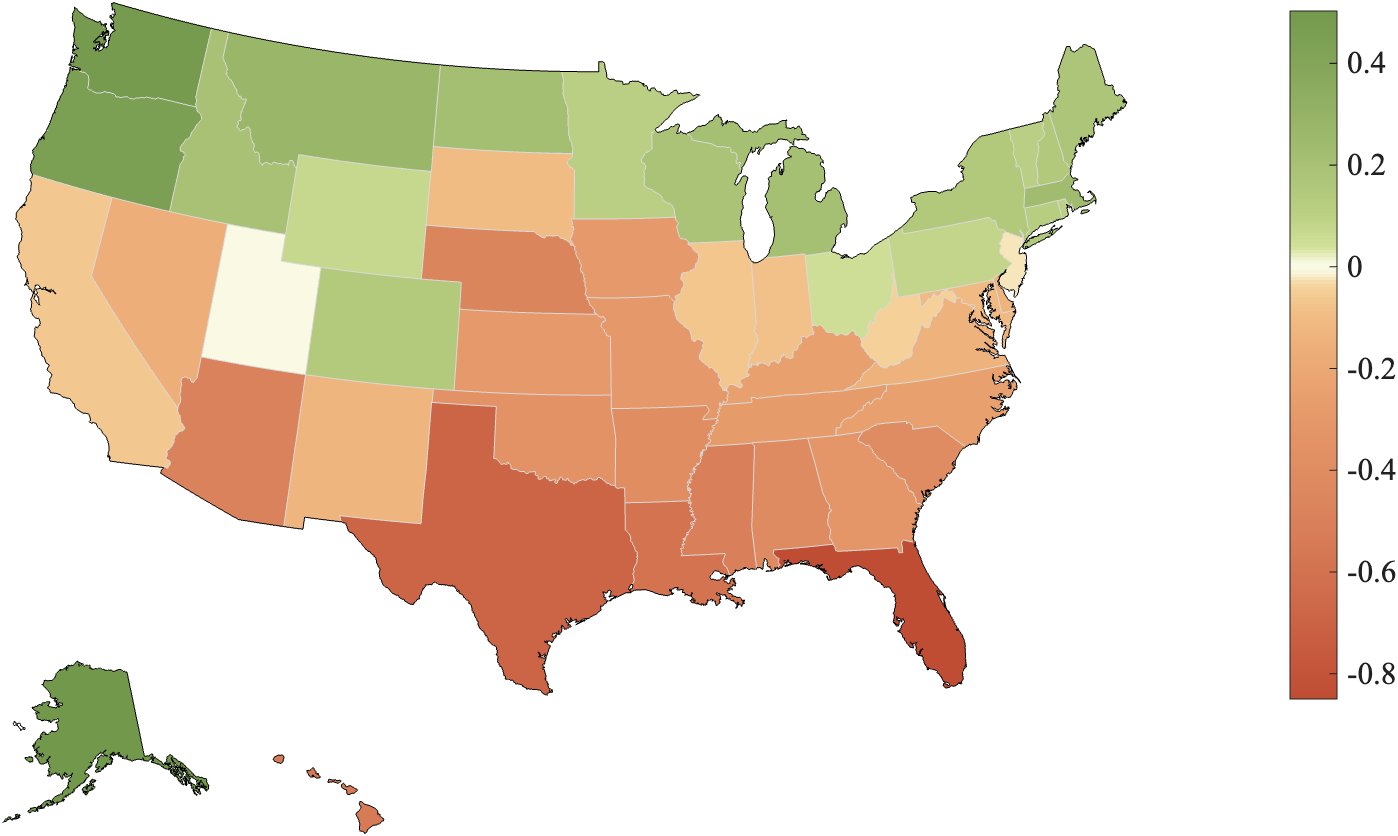
\includegraphics[width=\textwidth]{../Output/big_nu/graph_big_migration_did/transition_maps/transition_maps_wealth_income_ratio_changes.png}
  \end{minipage}
  \vspace{1em}
  \begin{minipage}[t]{0.4\textwidth}
    \centering
    \small{(c) $\Delta$ Local Population (\%)}
    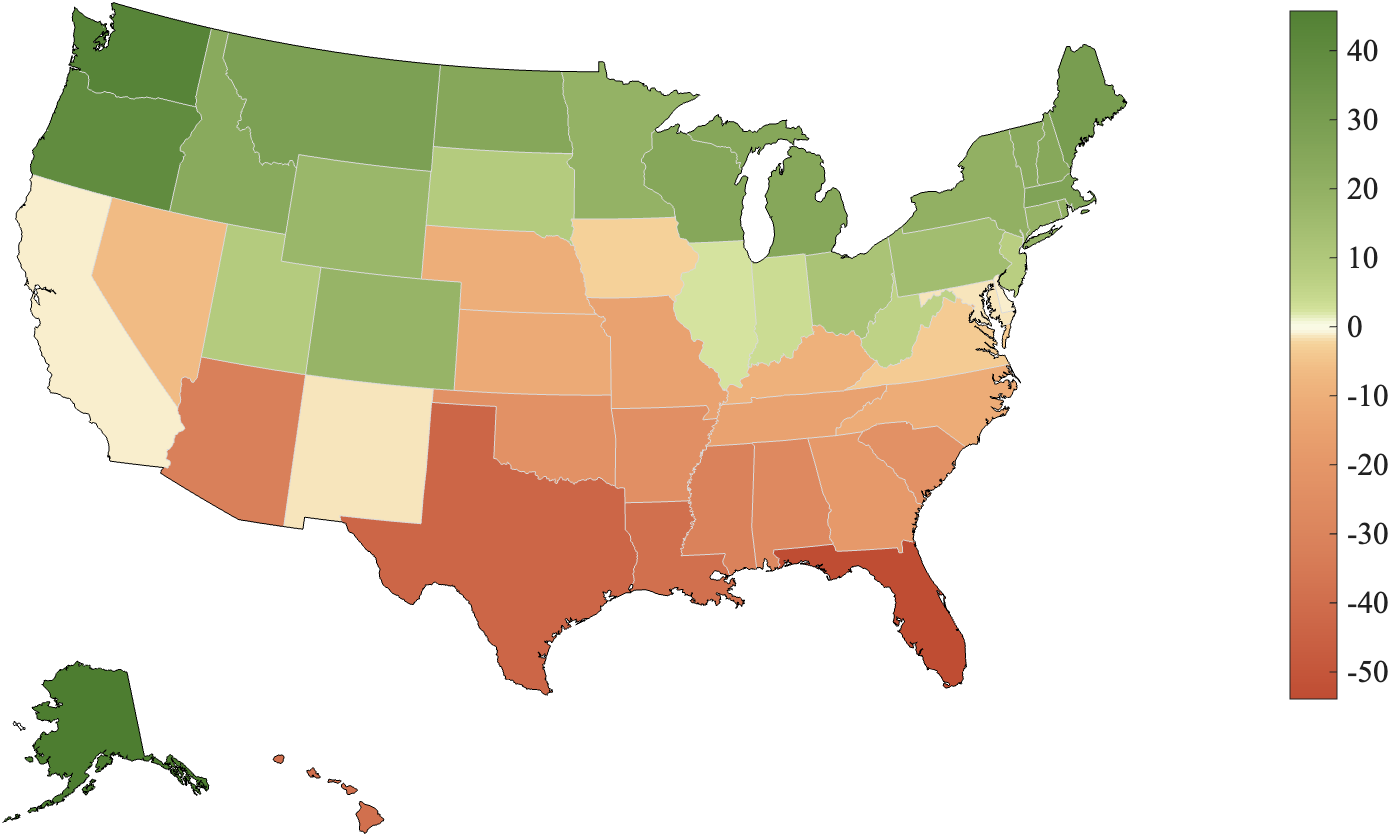
\includegraphics[width=\textwidth]{../Output/big_nu/graph_big_migration_did/transition_maps/transition_maps_local_pop_changes_pct.png}
  \end{minipage}\hfill
  \begin{minipage}[t]{0.4\textwidth}
    \centering
    \small{(d) $\Delta$ Mean Wealth (\%)}
    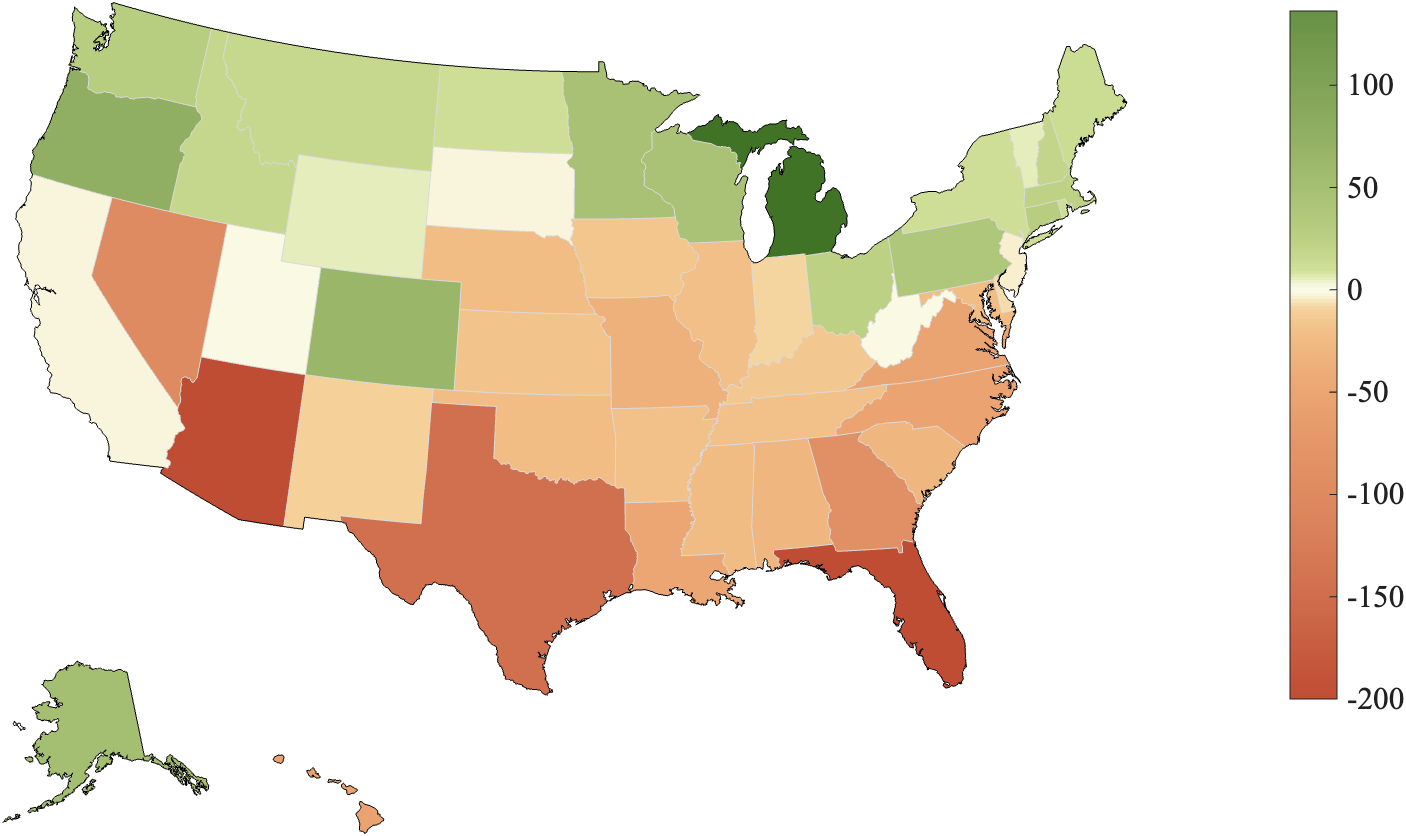
\includegraphics[width=\textwidth]{../Output/big_nu/graph_big_migration_did/transition_maps/transition_maps_pop_changes_pp.png}
  \end{minipage}
  \begin{minipage}{\textwidth}
  \vspace{0.5em}
  \footnotesize{\textbf{Note:} Spatial maps comparing the terminal steady state under 2100 climate parameters ($SS_\text{term}$) to the initial 2010 baseline steady state ($SS_\text{init}$) under Low Mig. Cost / 10\% moving cost reduction. Panel (a): change in mean Certainty Equivalent welfare $\Delta \text{CE}_\ell = \overline{\text{CE}}_{\ell, \text{term}} - \overline{\text{CE}}_{\ell, \text{init}}$. Panel (b): change in state wealth-to-earnings ratio $\Delta (W/Y)_\ell = (W/Y)_{\ell, \text{term}} - (W/Y)_{\ell, \text{init}}$. Panel (c): relative population percentage change $\Delta L_\ell\% = 100 \times (L_{\ell, \text{term}} - L_{\ell, \text{init}})/L_{\ell, \text{init}}$. Panel (d): percentage change in state mean per-capita wealth $\Delta \bar{a}_\ell\%$.} \end{minipage}
  \label{fig:low_mig_2}
\end{figure}

% 3. Welfare Inequality Maps only (1x2)
\begin{figure}[H]
  \centering
  \caption{Inequality Maps (Low Mig. Cost)}
  \begin{minipage}[t]{0.4\textwidth}
    \centering
    \small{(a) $\Delta$ Welfare Inequality (Std Dev \%)}
    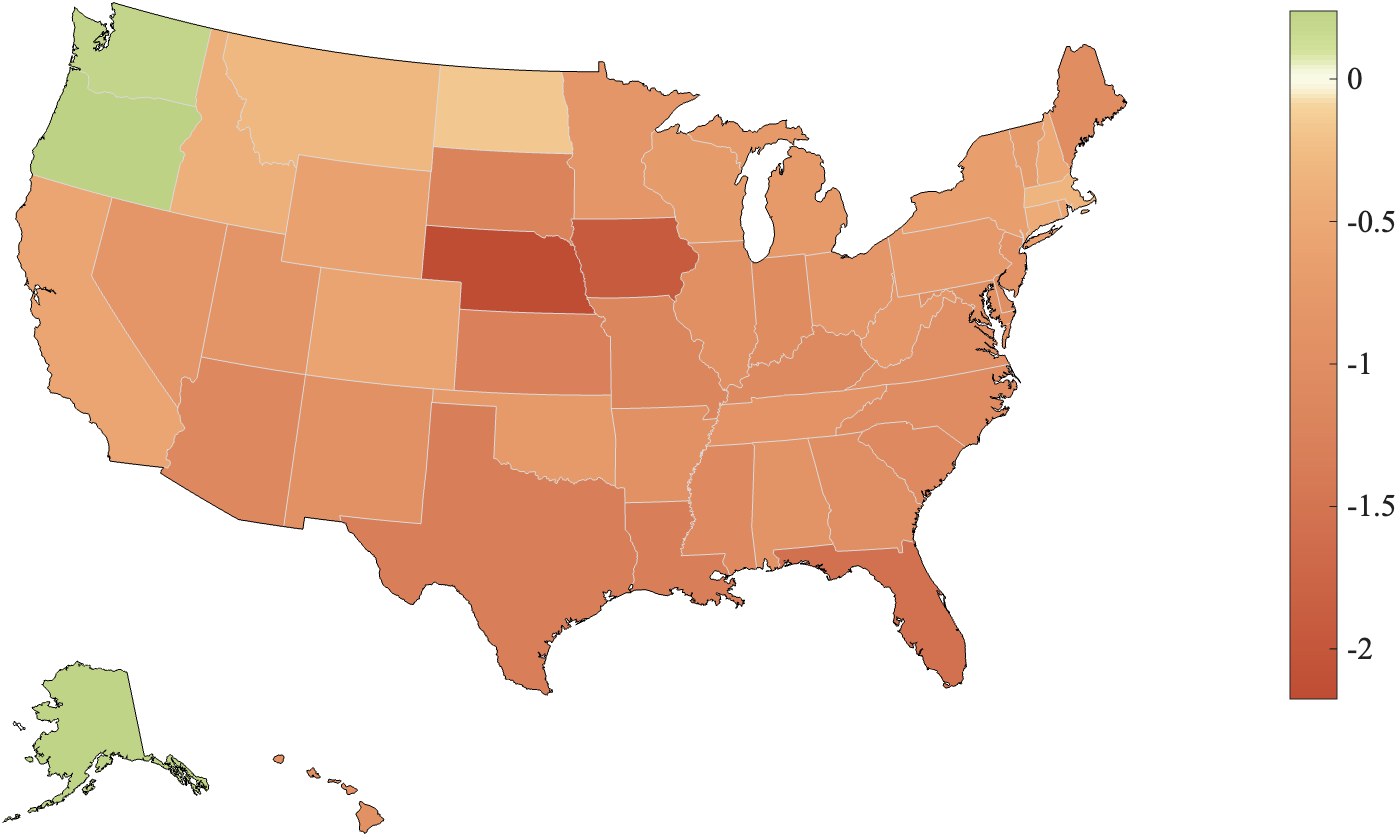
\includegraphics[width=\textwidth]{../Output/big_nu/graph_big_migration_did/welfare_wealth_inequality_maps/welfare_wealth_inequality_maps_welfare_inequality.png}
  \end{minipage}\hfill
  \begin{minipage}[t]{0.4\textwidth}
    \centering
    \small{(b) $\Delta$ Wealth Inequality (Std Dev \%)}
    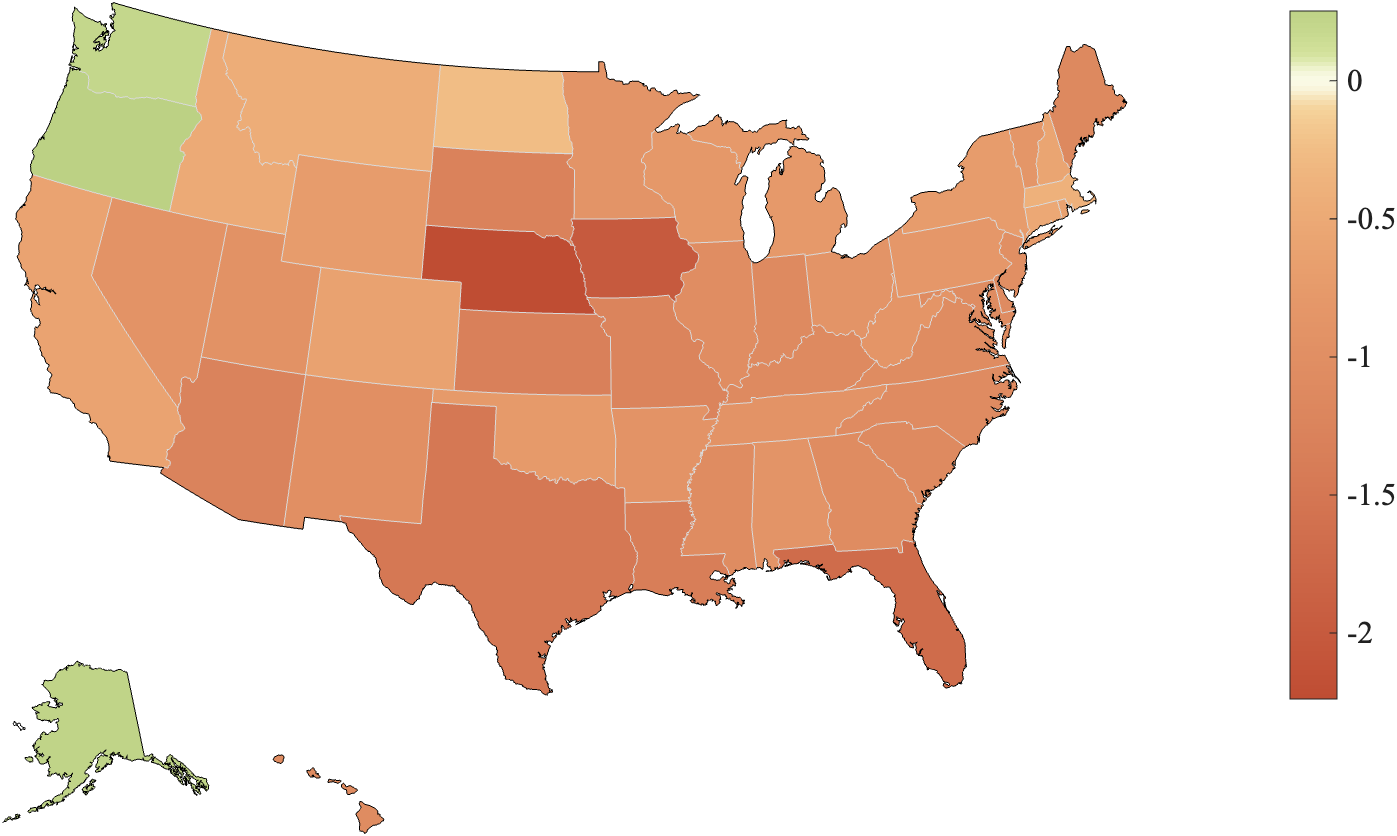
\includegraphics[width=\textwidth]{../Output/big_nu/graph_big_migration_did/welfare_wealth_inequality_maps/welfare_wealth_inequality_maps_wealth_inequality.png}
  \end{minipage}
  \begin{minipage}{\textwidth}
  \vspace{0.5em}
  \footnotesize{\textbf{Note:} Spatial inequality maps under Low Mig. Cost / 10\% moving cost reduction. Panel (a): percentage change in the within-state welfare standard deviation $\text{Var}_z(\text{CE}_\ell(z)) = \frac{1}{L_\ell} \sum_z \Lambda(\ell,z) [\text{CE}_\ell(z) - \overline{\text{CE}}_\ell]^2$ between the two steady states. Panel (b): percentage change in the within-state wealth standard deviation $\text{Var}_z(\bar{a}_\ell(z)) = \frac{1}{L_\ell} \sum_z \Lambda(\ell,z) [\bar{a}_\ell(z) - \bar{a}_\ell]^2$ between the two steady states.} \end{minipage}
  \label{fig:low_mig_3}
\end{figure}

\begin{figure}[H]
  \centering
    \caption{Wealth Decomposition (High Mig. Cost)}
  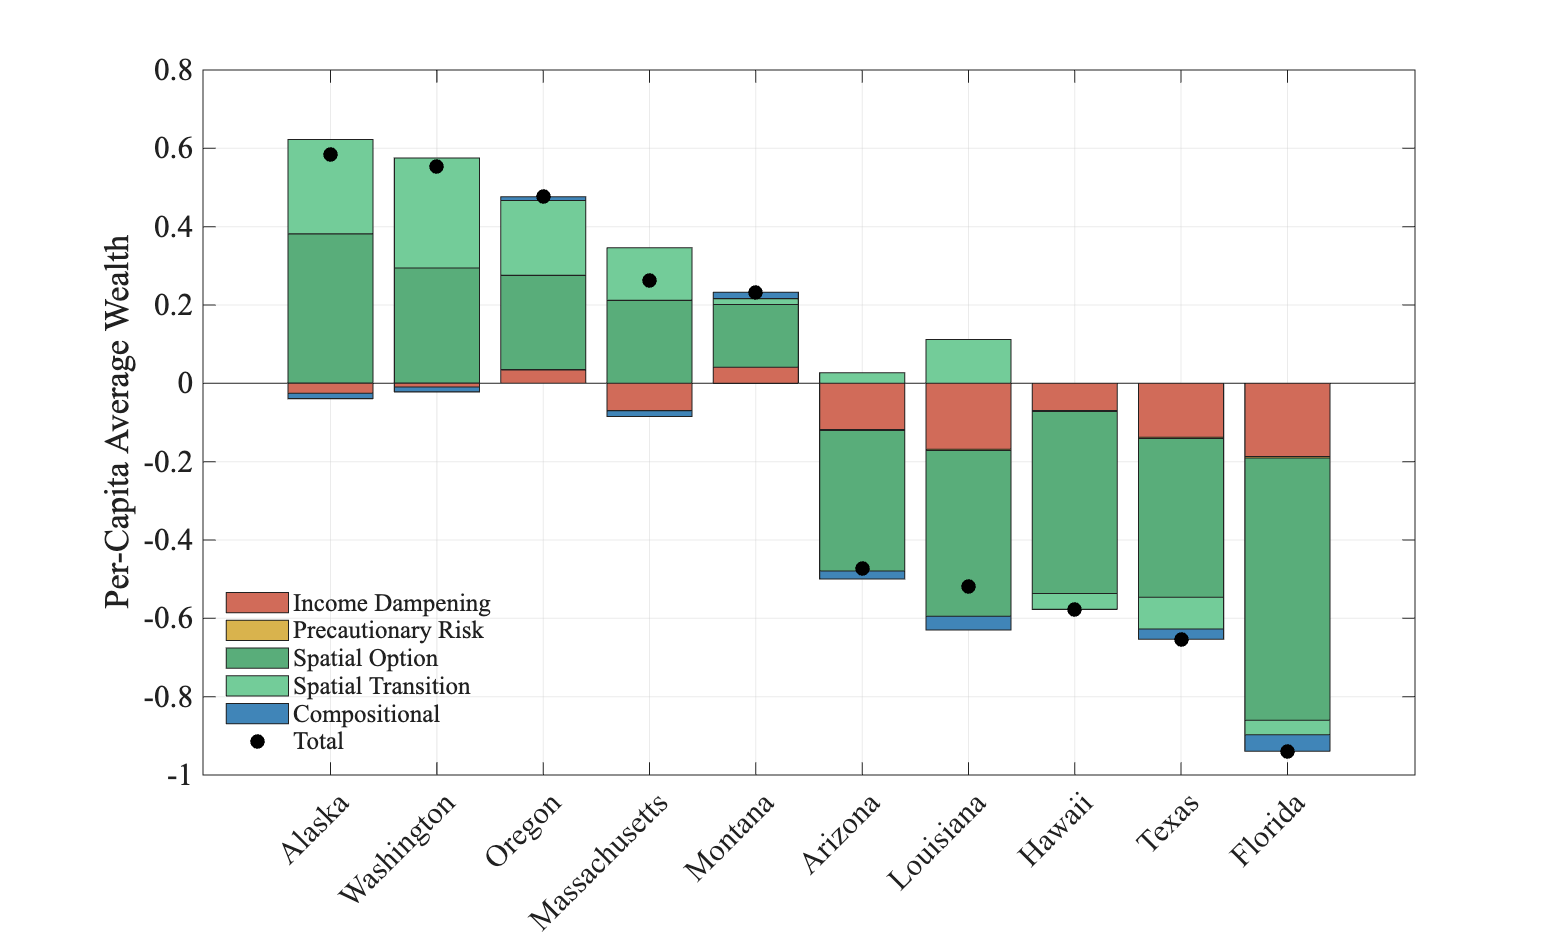
\includegraphics[width=\textwidth]{../Output/big_nu/graph_big_migration_did/exact_percapita_decomposition_bar_did_big_migration_Treat_vs_Ctrl.png}
  \begin{minipage}{\textwidth}
  \vspace{0.5em}
  \footnotesize{\textbf{Note:} Structural shift-share decomposition of the state-level per-capita wealth change $\Delta \bar{a}_\ell = \bar{a}_{\ell, \text{term}} - \bar{a}_{\ell, \text{init}}$ under High Mig. Cost into five margins: (1) Income Dampening: savings adjustments to income changes evaluated at the baseline autarky network; (2) Precautionary Risk: shifts in savings due to altered income variance evaluated at autarky; (3) Spatial + Amenity: network premium from accumulating wealth over the baseline spatial network versus autarky; (4) Spatial Transition: change in the migration network evaluated at the new savings behaviour; (5) Compositional: changes in local productivity shares.}
  \end{minipage}
  \label{fig:high_mig_4}
\end{figure}

\subsection{Variance Shocks}

Climate change is expected to not only have an effect on the level of the fundamentals in an economy but also on their uncertainty due to extreme events. However, the study by \citet{hsiang_estimating_2017} does not provide uncertainty estimates on climate damages, but it is possible to construct a variance shock scenario by assuming that agents anticipate a future increase in the variance of idiosyncratic shocks. This can be modelled as a localised increase in variance $\sigma^2_{\eta, t}$ in certain regions or sectors, capturing the idea that climate change increases the frequency of extreme events such as storms, droughts, floods, wildfires, or others that agents cannot anticipate, thereby increasing the idiosyncratic risk they face. Small variations (on the order of 3–4\%) in $\sigma^2_{\eta, t}$ have little effect on agent behaviour, and these results are not reported. The magnitude of the variance shock in the simulations is set proportionally to the magnitude of the wage shock, with a multiplier of 50 to generate significant effects: $\Delta \sigma^2_{\eta, \ell} = 50 \cdot |\Delta w_\ell|$.

The following scenario was thus considered: More unpredictable extreme events affect individuals due to climate change. The variance of idiosyncratic shocks increases progressively and linearly until reaching its maximum level in 2100 and remains there permanently.
    \begin{equation}
        \sigma^2_{\eta, \ell, t} = \bar{\sigma}^2_{\eta, \ell} \left( 1 + 50 \cdot |\Delta w_\ell| \cdot \left(\frac{t}{T_{\text{shock}}}\right) \right)
    \end{equation}

Figure~\ref{fig:variance_shock_map} illustrates the spatial distribution of the variance increase at its maximum level.
\begin{figure}[!htb]
  \centering
  \caption{$\Delta \sigma^2_\eta$ (Peak increase, \%)}
  \label{fig:variance_shock_map}
  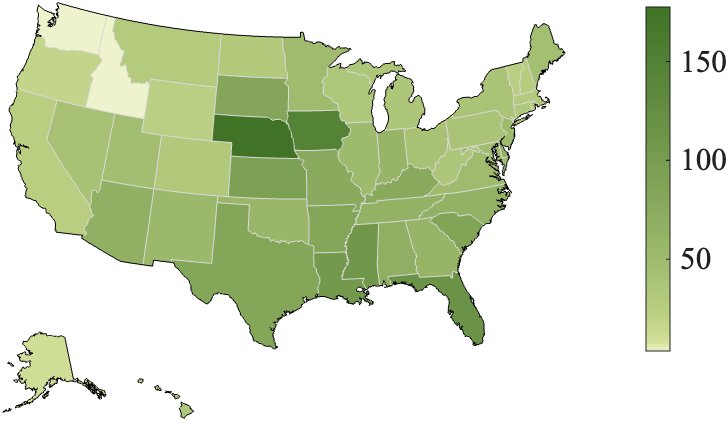
\includegraphics[width=0.5\textwidth]{../Output/big_nu/graph_uncertainty_variance_shocks/variance_map.png}
  \begin{minipage}{\textwidth}
  \vspace{0.5em}
  \footnotesize{\textbf{Note:} Spatial distribution of the climate-induced idiosyncratic shock variance increase $\Delta \sigma^2_{\eta,\ell} = 50 \cdot |\Delta w_\ell|$ (in \%) designed to capture the uncertainty of climate change damage.} \end{minipage}
\end{figure}

\begin{figure}[H]
  \centering
  \caption{Dynamic Moments (Variance Shock)}
  \begin{minipage}[t]{0.4\textwidth}
    \centering
    \small{(a) Earnings}
    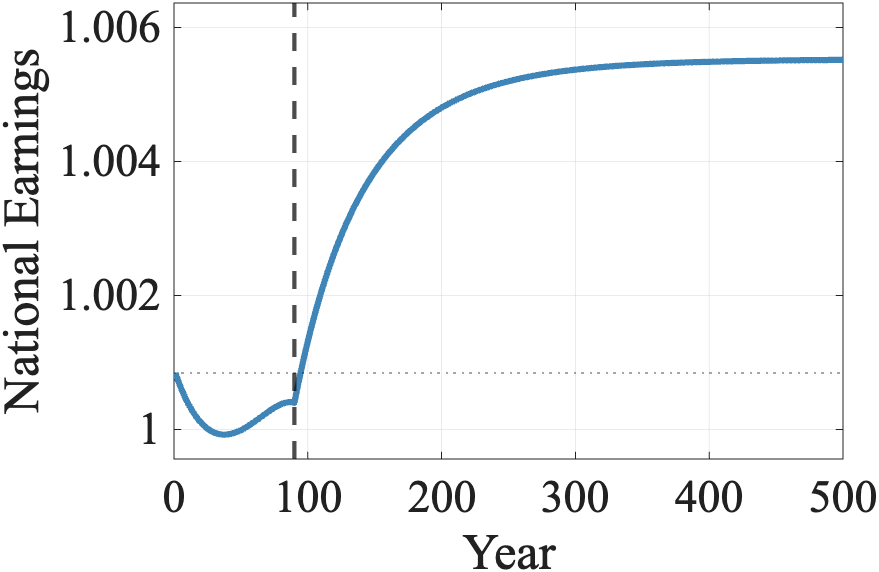
\includegraphics[width=\textwidth]{../Output/big_nu/graph_uncertainty_variance_shocks/dynamic_moments/dynamic_moments_national_earnings.png}
  \end{minipage}\hfill
  \begin{minipage}[t]{0.4\textwidth}
    \centering
    \small{(b) Mobility}
    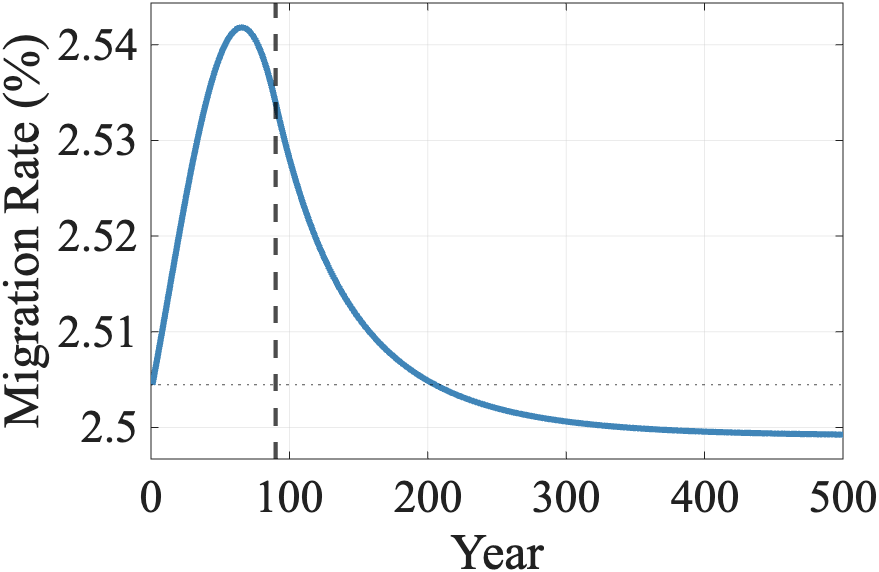
\includegraphics[width=\textwidth]{../Output/big_nu/graph_uncertainty_variance_shocks/dynamic_moments/dynamic_moments_national_mobility.png}
  \end{minipage} \\[2ex]
  \begin{minipage}[t]{0.4\textwidth}
    \centering
    \small{(c) Wealth}
    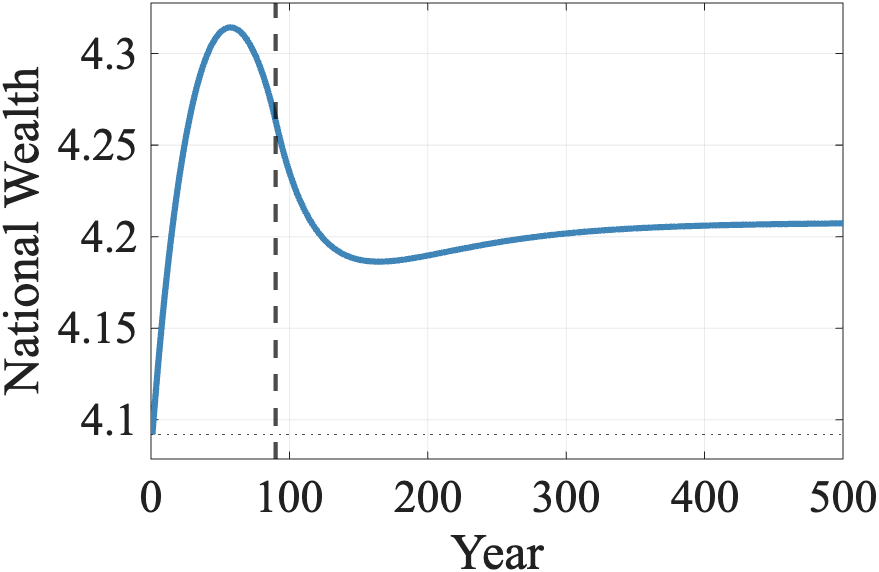
\includegraphics[width=\textwidth]{../Output/big_nu/graph_uncertainty_variance_shocks/dynamic_moments/dynamic_moments_national_wealth.png}
  \end{minipage}\hfill
  \begin{minipage}[t]{0.4\textwidth}
    \centering
    \small{(d) W/Y Ratio}
    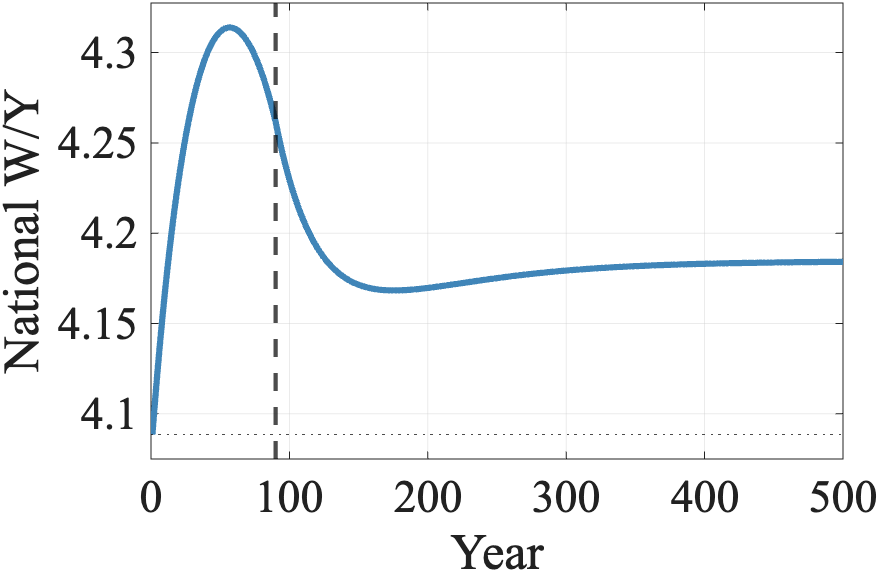
\includegraphics[width=\textwidth]{../Output/big_nu/graph_uncertainty_variance_shocks/dynamic_moments/dynamic_moments_national_wy.png}
  \end{minipage} \begin{minipage}{\textwidth} 
  \vspace{0.5em}
  \footnotesize{\textbf{Note:} Aggregate macroeconomic time series when introducing climate change variance-induced uncertainty, 2010--2500+. Panel (a): national total disposable labour earnings. Panel (b): national gross annual inter-state migration rate. Panel (c): total national wealth holdings. Panel (d): aggregate wealth-to-earnings ratio.} \end{minipage}
\end{figure}

\begin{figure}[H]
  \centering
  \caption{Transition Maps (Variance Shock)}
  \begin{minipage}[t]{0.4\textwidth}
    \centering
    \small{(a) $\Delta$ Mean Welfare (CE)}
    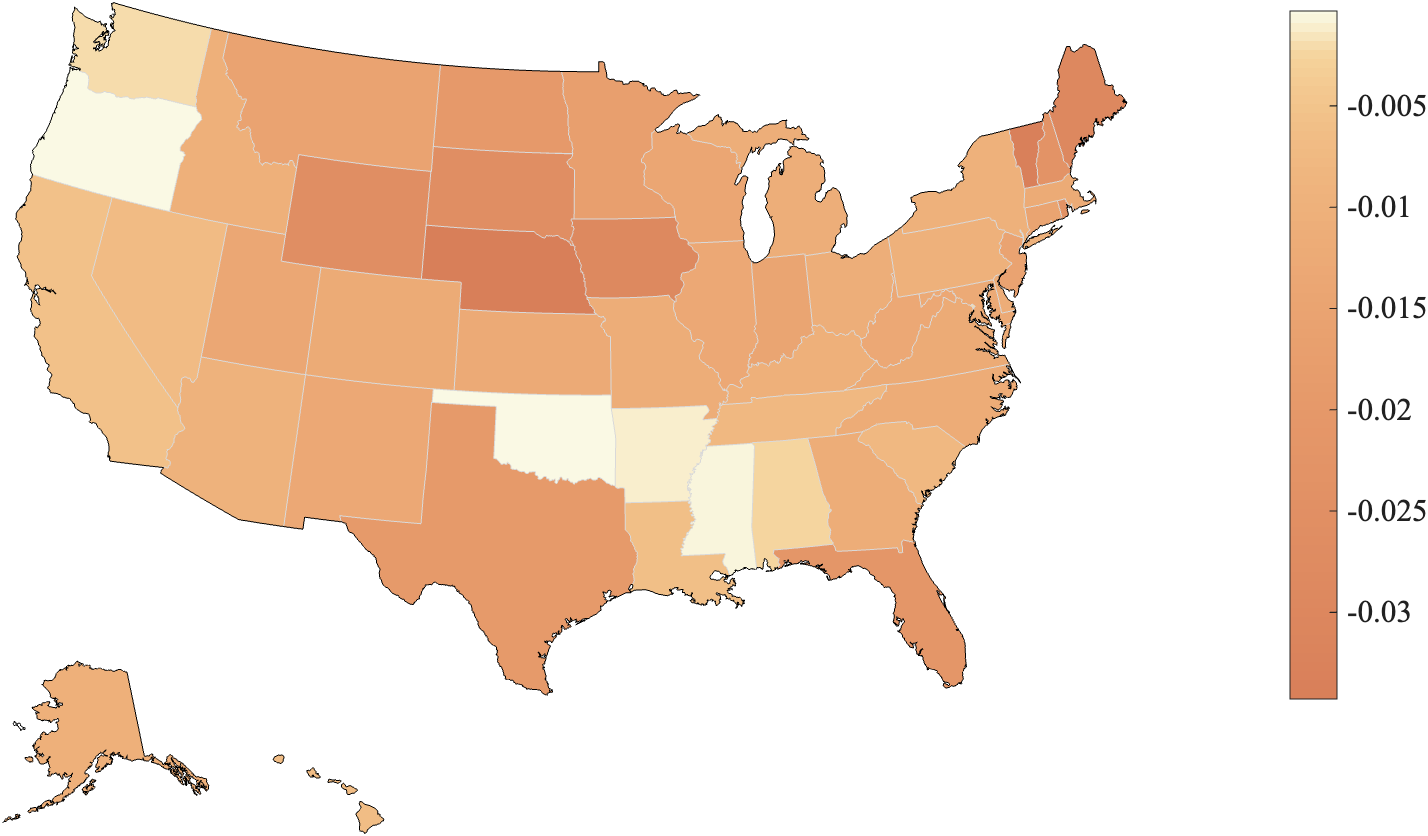
\includegraphics[width=\textwidth]{../Output/big_nu/graph_uncertainty_variance_shocks/transition_maps/transition_maps_delta_mean_welfare_ce.png}
  \end{minipage}\hfill
  \begin{minipage}[t]{0.4\textwidth}
    \centering
    \small{(b) $\Delta$ W/Y Ratio in level}
    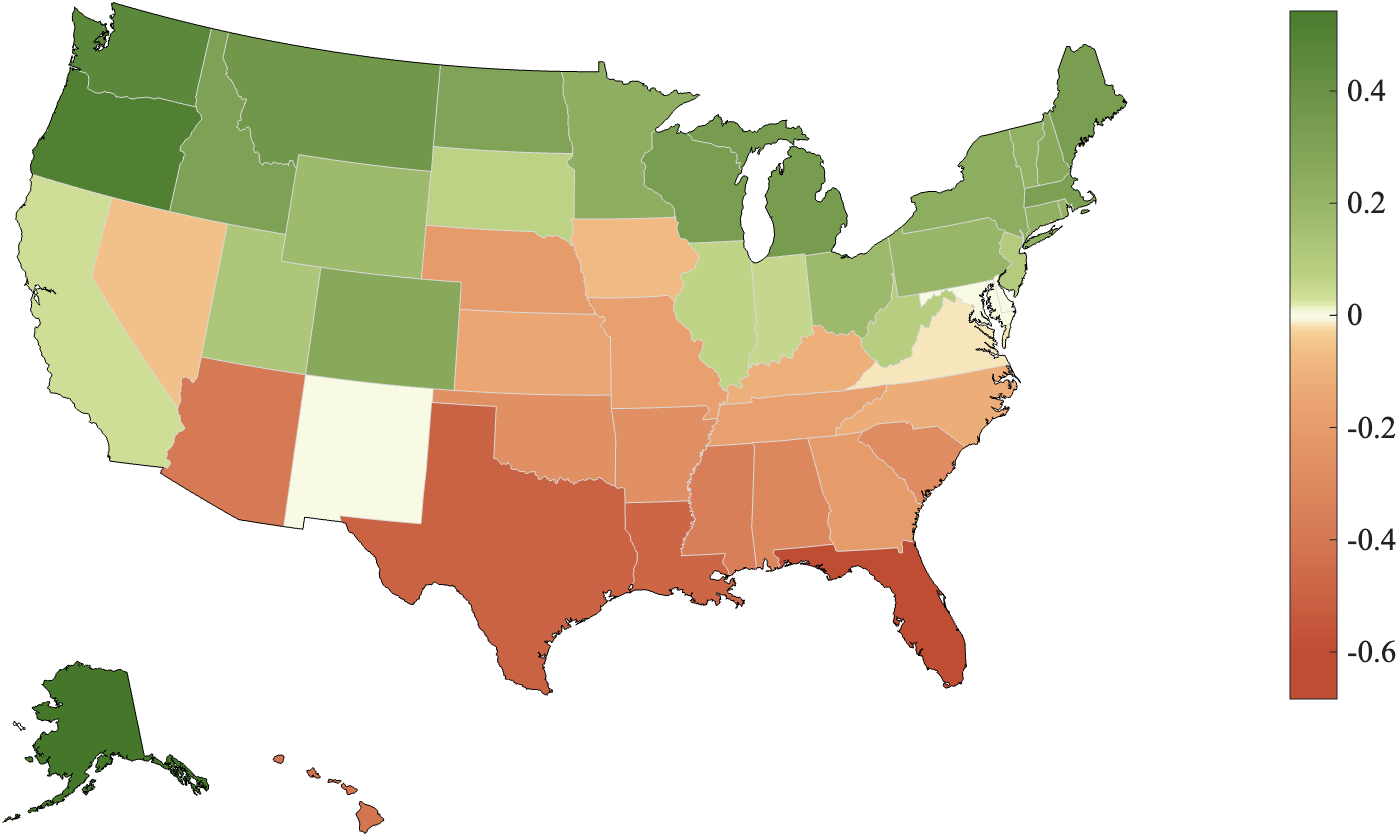
\includegraphics[width=\textwidth]{../Output/big_nu/graph_uncertainty_variance_shocks/transition_maps/transition_maps_wealth_income_ratio_changes.png}
  \end{minipage}\\[2ex]
  \begin{minipage}[t]{0.4\textwidth}
    \centering
    \small{(c) $\Delta$ Local Population (\%)}
    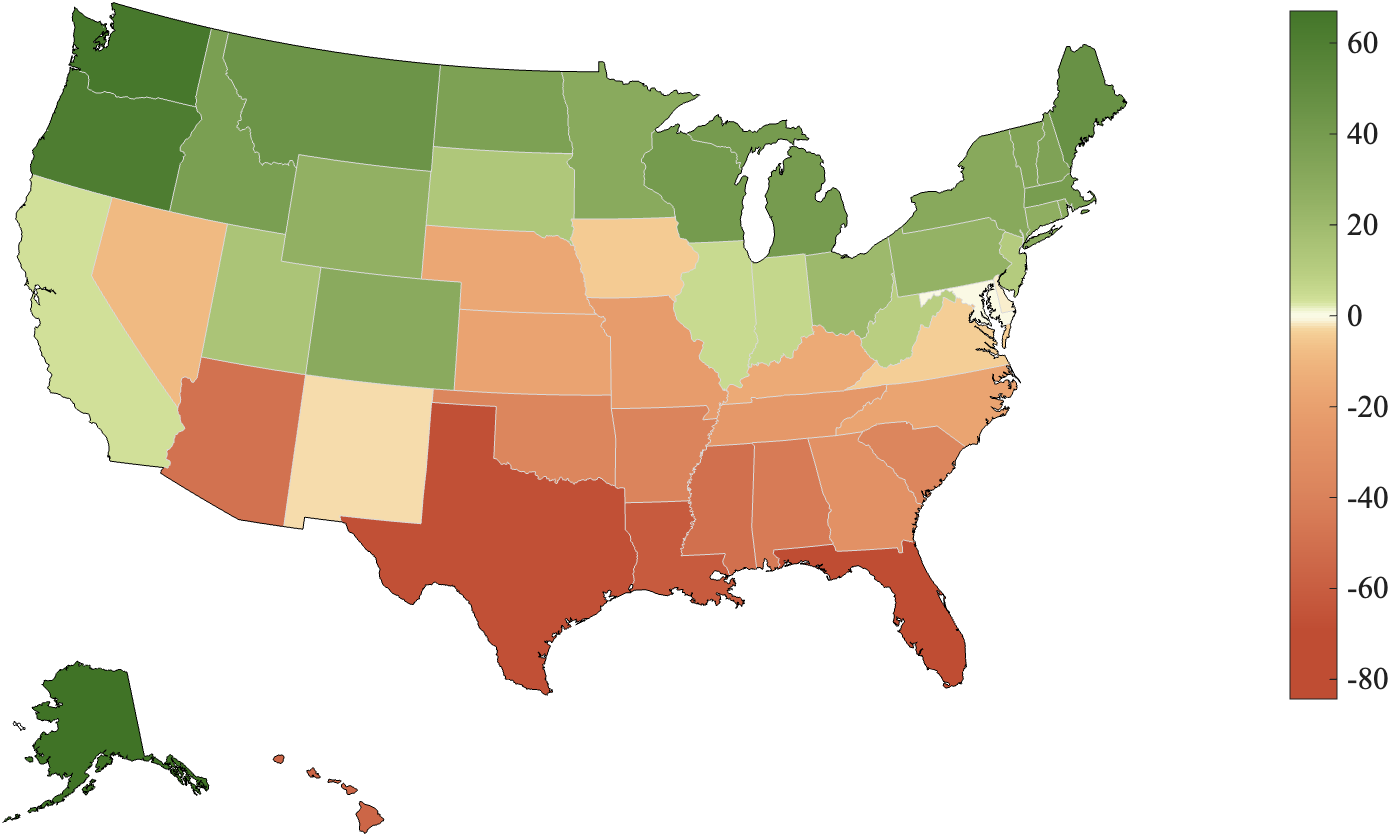
\includegraphics[width=\textwidth]{../Output/big_nu/graph_uncertainty_variance_shocks/transition_maps/transition_maps_local_pop_changes_pct.png}
  \end{minipage}\hfill
  \begin{minipage}[t]{0.4\textwidth}
    \centering
    \small{(d) $\Delta$ Mean Wealth (\%)}
    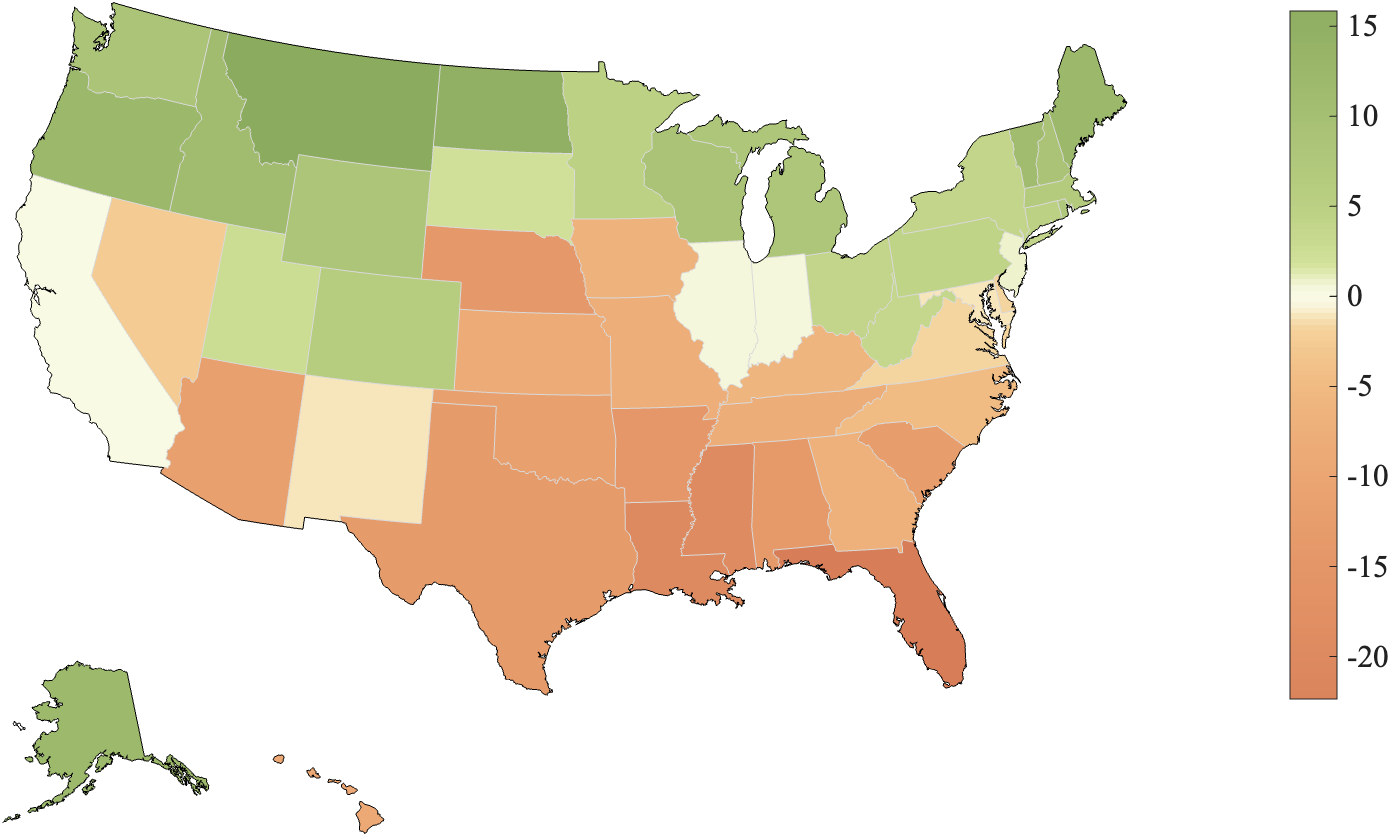
\includegraphics[width=\textwidth]{../Output/big_nu/graph_uncertainty_variance_shocks/transition_maps/transition_maps_pop_changes_pp.png}
  \end{minipage}
   \begin{minipage}{\textwidth}
  \vspace{0.5em}
  \footnotesize{\textbf{Note:} Spatial maps comparing the terminal steady state under 2100 climate parameters ($SS_\text{term}$) to the initial 2010 baseline steady state ($SS_\text{init}$) when introducing climate change variance-induced uncertainty. Panel (a): change in mean Certainty Equivalent welfare. Panel (b): change in state wealth-to-earnings ratio. Panel (c): relative population percentage change. Panel (d): percentage change in state mean per-capita wealth $\Delta \bar{a}_\ell\%$.} \end{minipage}
\end{figure}

\begin{figure}[H]
  \centering
    \caption{Wealth's Change Decomposition (Variance Shock)}
  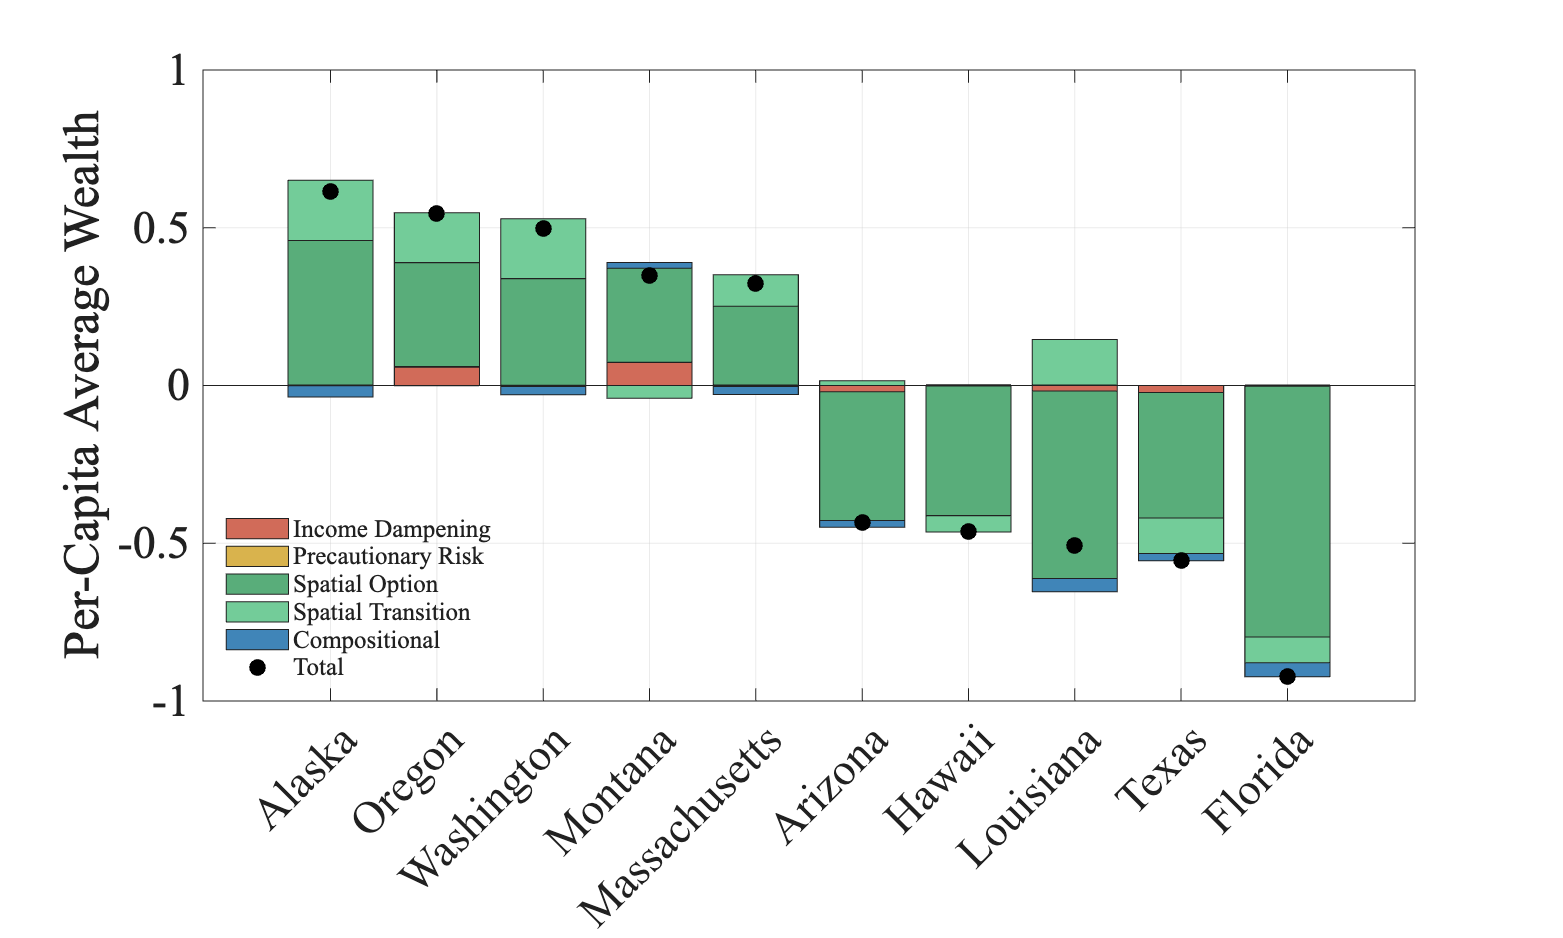
\includegraphics[width=\textwidth]{../Output/big_nu/graph_uncertainty_variance_shocks/exact_percapita_decomposition_bar_no_counterfactual_no_counterfactual.png}
  \begin{minipage}{\textwidth}
  \vspace{0.5em}
  \footnotesize{\textbf{Note:} Structural shift-share decomposition of the state-level per-capita wealth change $\Delta \bar{a}_\ell = \bar{a}_{\ell, \text{term}} - \bar{a}_{\ell, \text{init}}$ with climate change variance-induced uncertainty into five margins: (1) Income Dampening (2) Precautionary Risk (3) Spatial option (4) Spatial Transition (5) Compositional.}
  \end{minipage}
\end{figure}

\begin{figure}[H]
  \centering
  \caption{Inequality Maps and Transition (Variance Shock)}
  \begin{minipage}[t]{0.4\textwidth}
    \centering
    \small{(a) $\Delta$ Welfare Inequality (Std Dev \%)}
    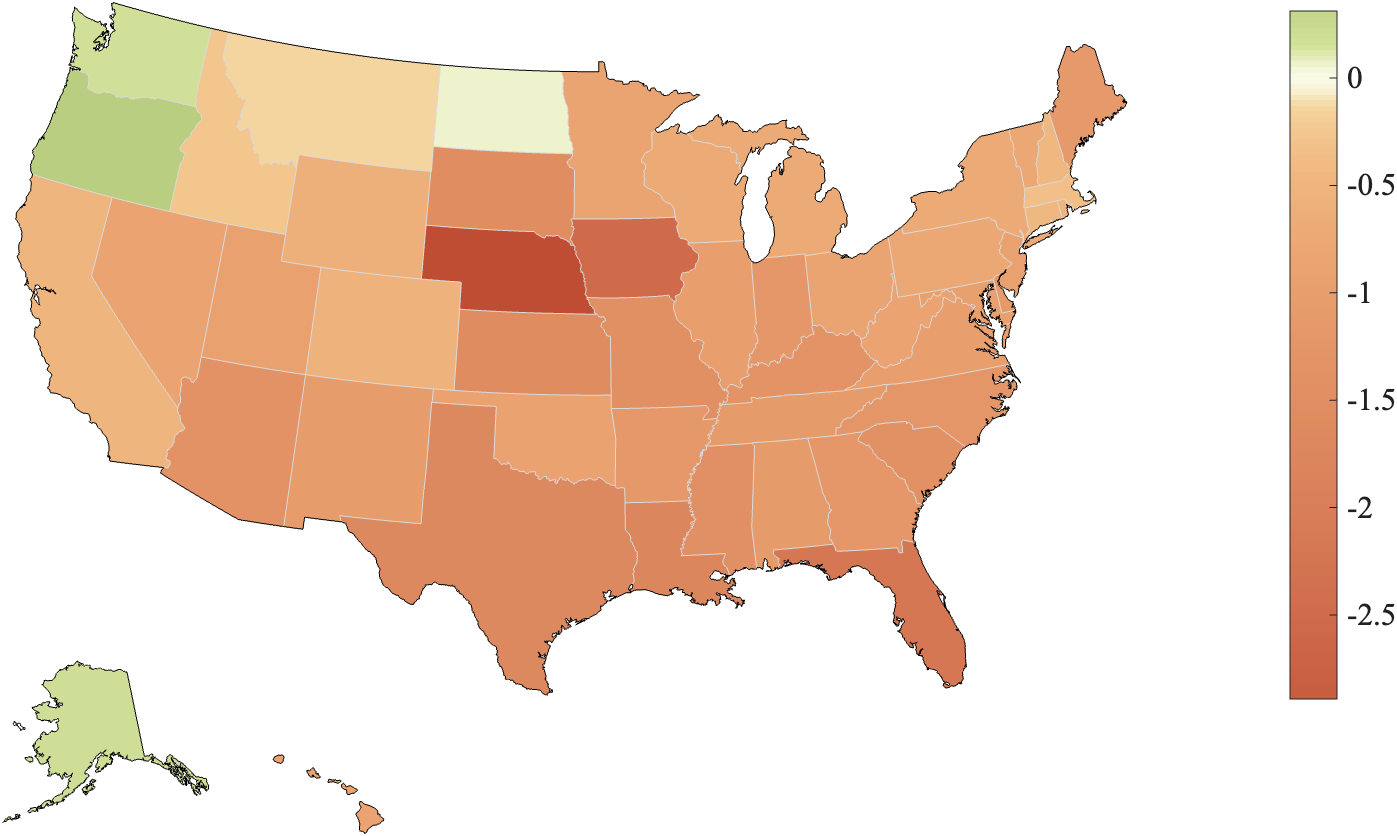
\includegraphics[width=\textwidth]{../Output/big_nu/graph_uncertainty_variance_shocks/welfare_wealth_inequality_maps/welfare_wealth_inequality_maps_welfare_inequality.png}
  \end{minipage}\hfill
  \begin{minipage}[t]{0.4\textwidth}
    \centering
    \small{(b) $\Delta$ Wealth Inequality (Std Dev \%)}
    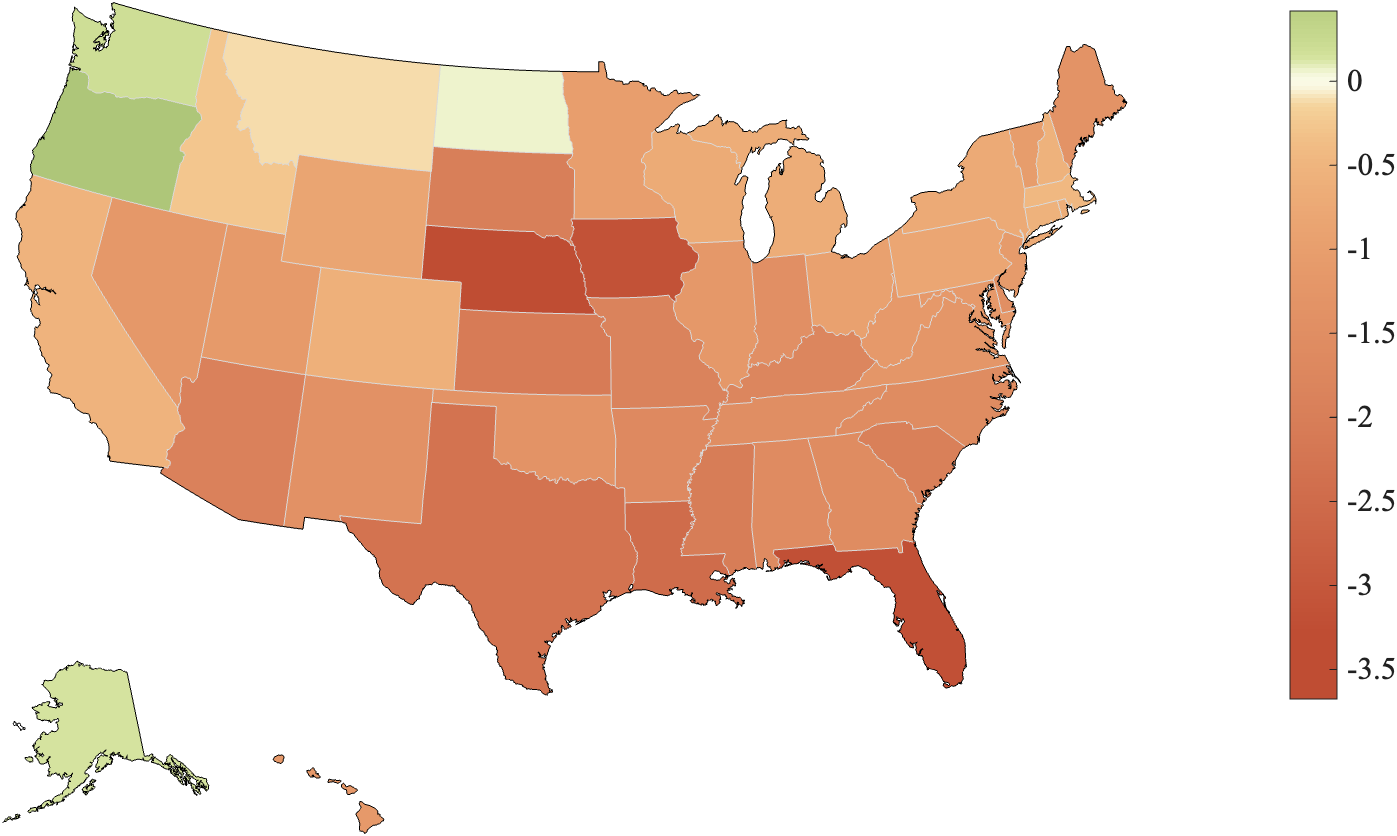
\includegraphics[width=\textwidth]{../Output/big_nu/graph_uncertainty_variance_shocks/welfare_wealth_inequality_maps/welfare_wealth_inequality_maps_wealth_inequality.png}
  \end{minipage}
  \vspace{1em}
  \begin{minipage}[t]{0.4\textwidth}
    \centering
    \small{(c) $\Delta$ Welfare Inequality (Std Dev \%)}
    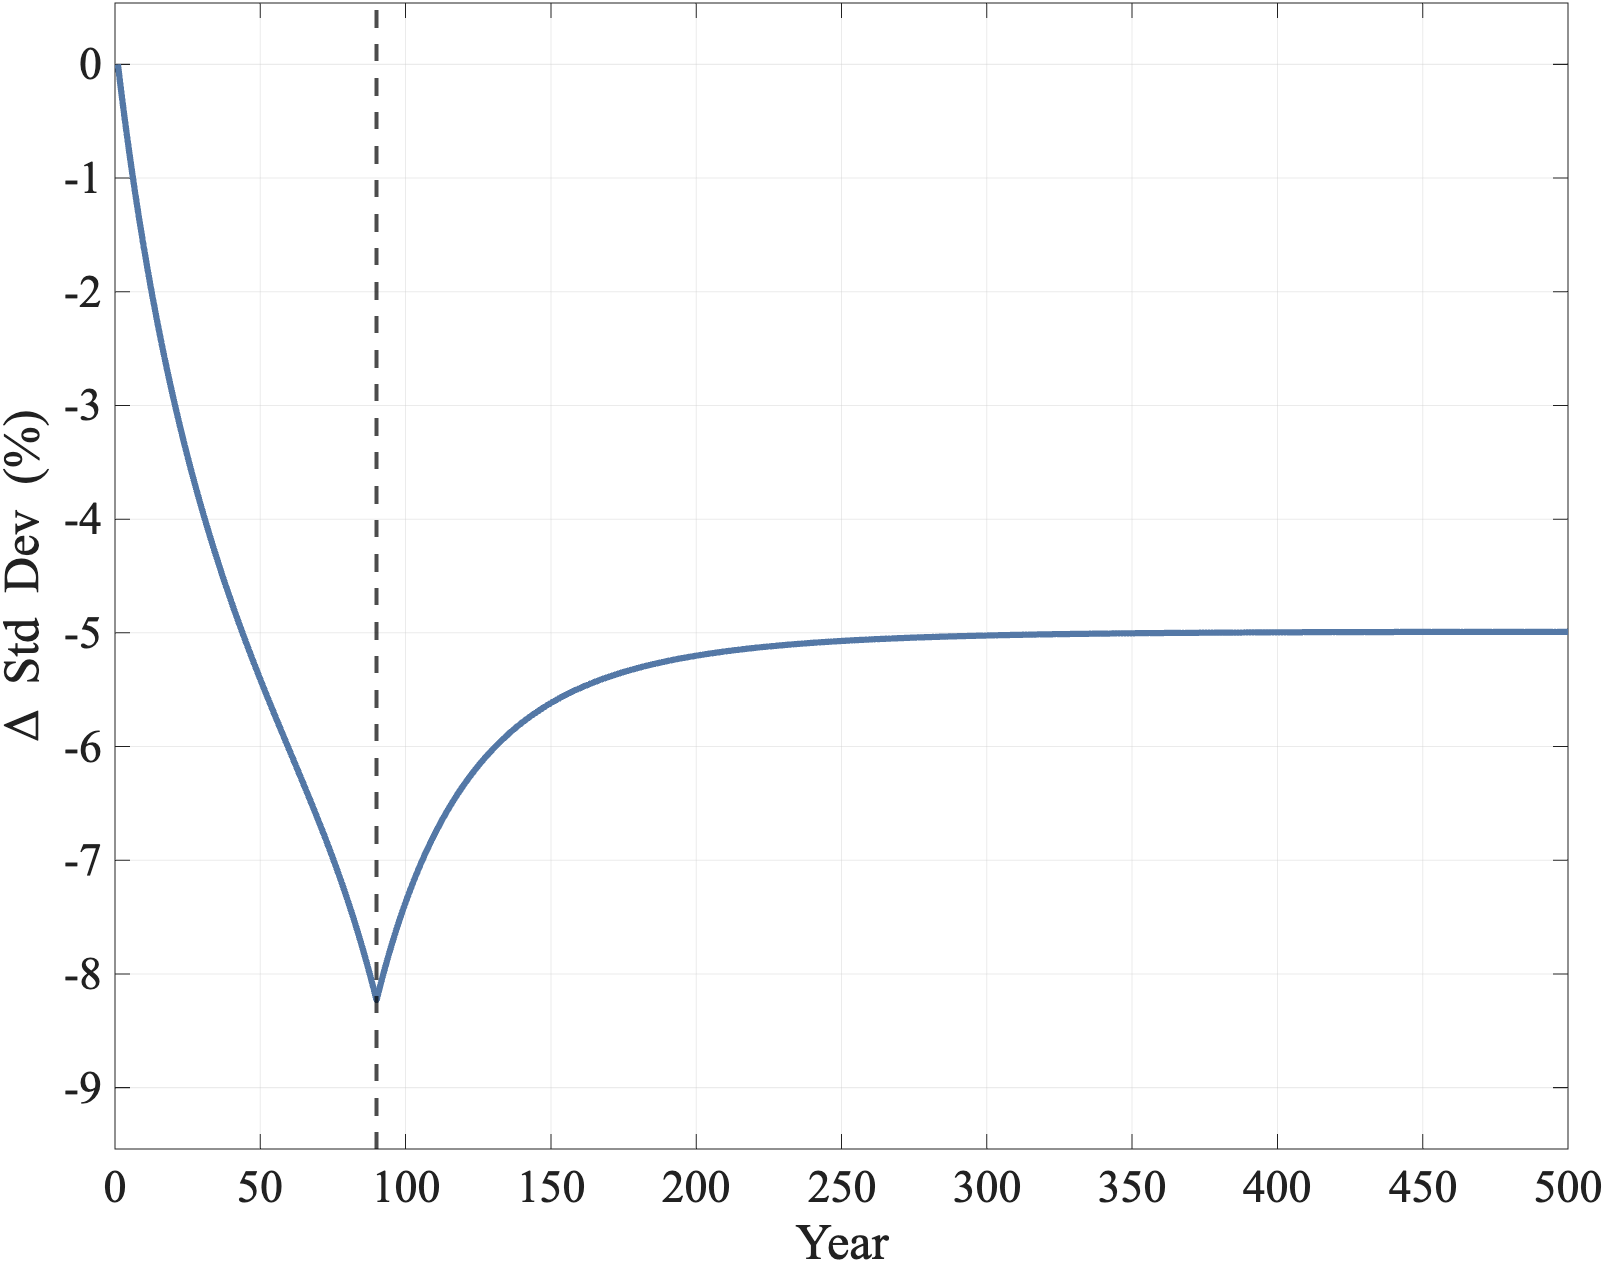
\includegraphics[width=\textwidth]{../Output/big_nu/graph_uncertainty_variance_shocks/welfare_transition/welfare_transition_welfare_inequality.png}
  \end{minipage}\hfill
  \begin{minipage}[t]{0.4\textwidth}
    \centering
    \small{(d) $\Delta$ Wealth Inequality (Std Dev \%)}
    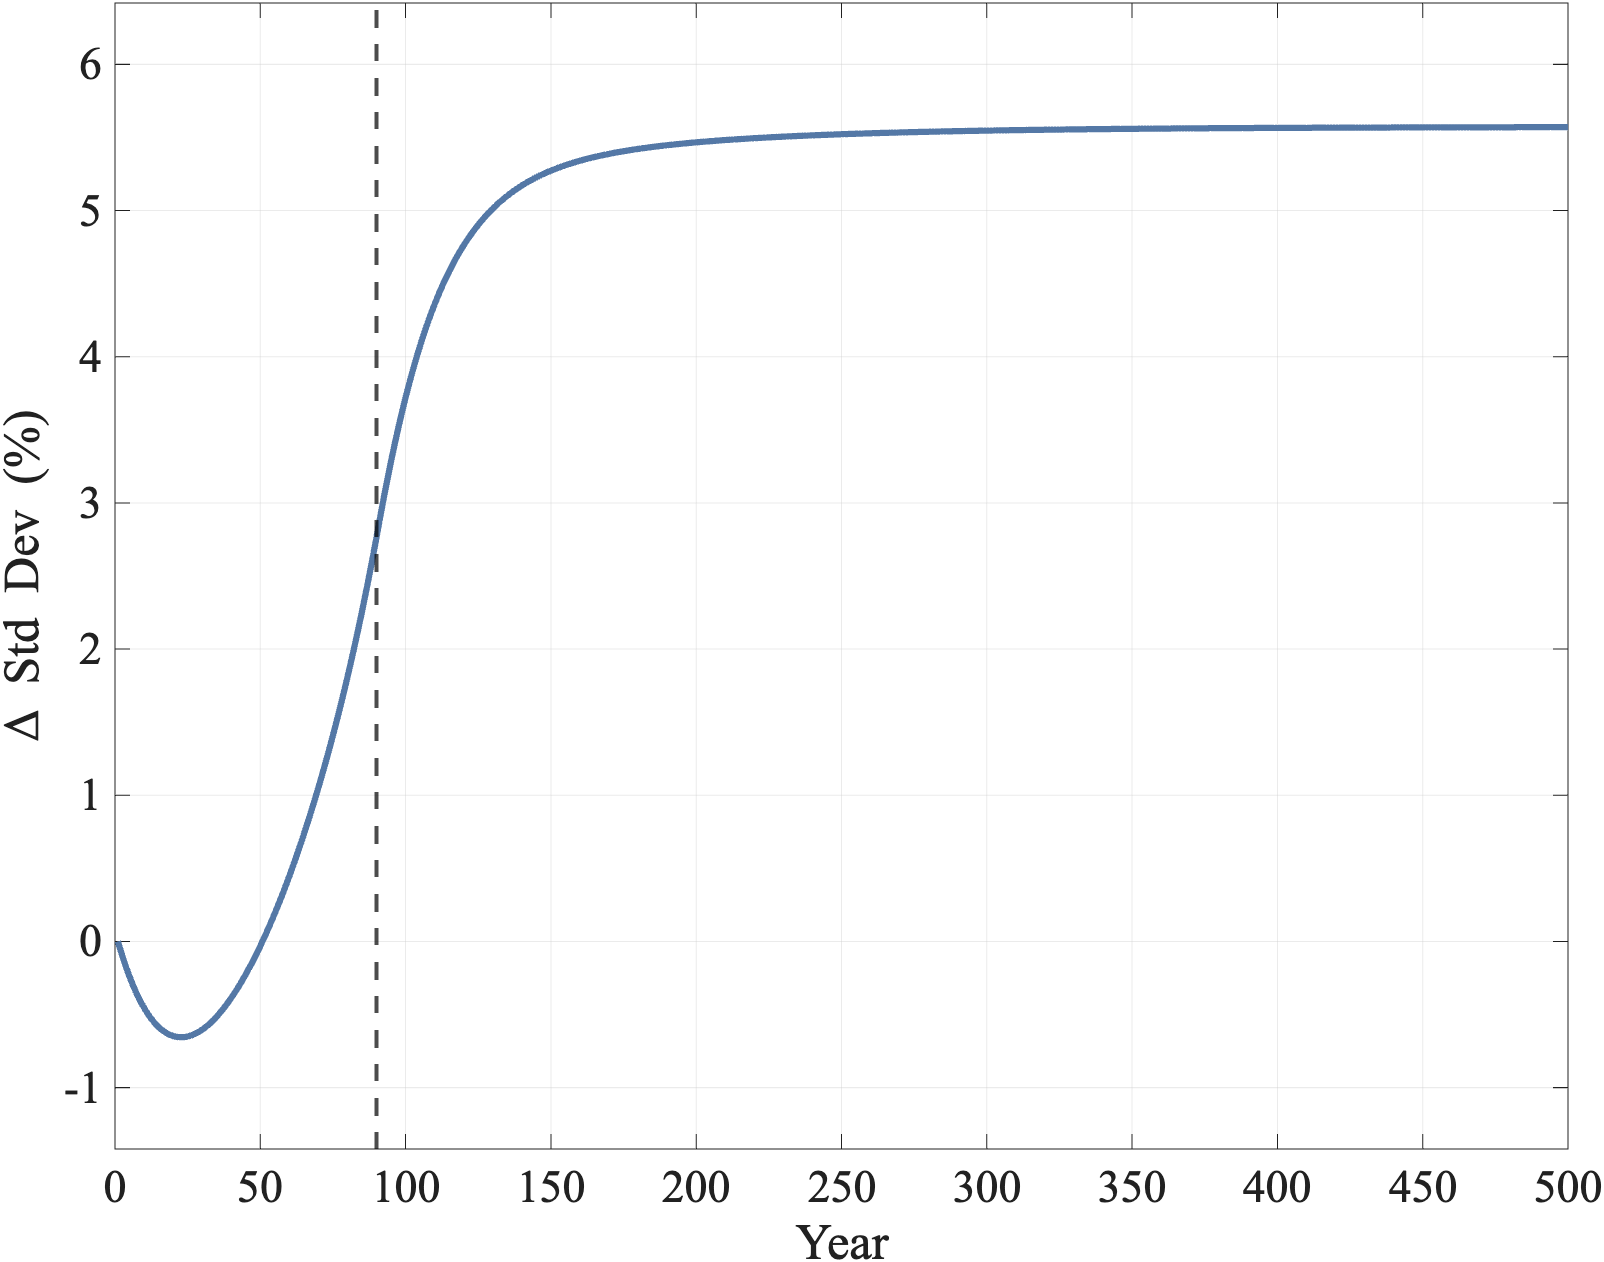
\includegraphics[width=\textwidth]{../Output/big_nu/graph_uncertainty_variance_shocks/welfare_transition/welfare_transition_wealth_inequality.png}
  \end{minipage}
  \begin{minipage}{\textwidth}
  \vspace{0.5em}
  \footnotesize{\textbf{Note:} Spatial and dynamic inequality metrics with climate change variance-induced uncertainty. Panel (a): percentage change in the within-state welfare standard deviation between the two steady states. Panel (b): percentage change in the within-state wealth standard deviation between the two steady states. Panel (c): dynamic transition of national cross-state welfare inequality. Panel (d): dynamic transition of national cross-state wealth inequality.} \end{minipage}
\end{figure}

\subsection{Variance Shocks No Migration}

% 1. Dynamic Moments Diff (4 in a line)
\begin{figure}[H]
  \centering
  \caption{Dynamic Moments Diff (Variance Shocks No Migration (DiD))}
  \begin{minipage}[t]{0.4\textwidth}
    \centering
    \small{(a) Earnings Diff}
    \includegraphics[width=\textwidth]{../Output/big_nu/graph_uncertainty_variance_shocks_no_migration_did/did_dynamic_moments_diff_earnings.png}
  \end{minipage}\hfill
  \begin{minipage}[t]{0.4\textwidth}
    \centering
    \small{(b) Migration Diff}
    \includegraphics[width=\textwidth]{../Output/big_nu/graph_uncertainty_variance_shocks_no_migration_did/did_dynamic_moments_diff_migration.png}
  \end{minipage} \\[2ex]
  \begin{minipage}[t]{0.4\textwidth}
    \centering
    \small{(c) Wealth Diff}
    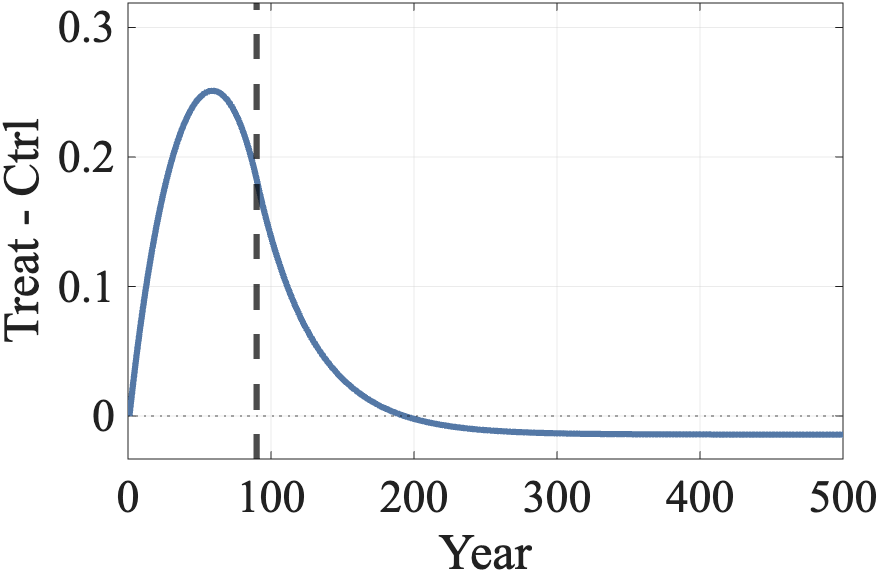
\includegraphics[width=\textwidth]{../Output/big_nu/graph_uncertainty_variance_shocks_no_migration_did/did_dynamic_moments_diff_wealth.png}
  \end{minipage}\hfill
  \begin{minipage}[t]{0.4\textwidth}
    \centering
    \small{(d) W/Y Diff}
    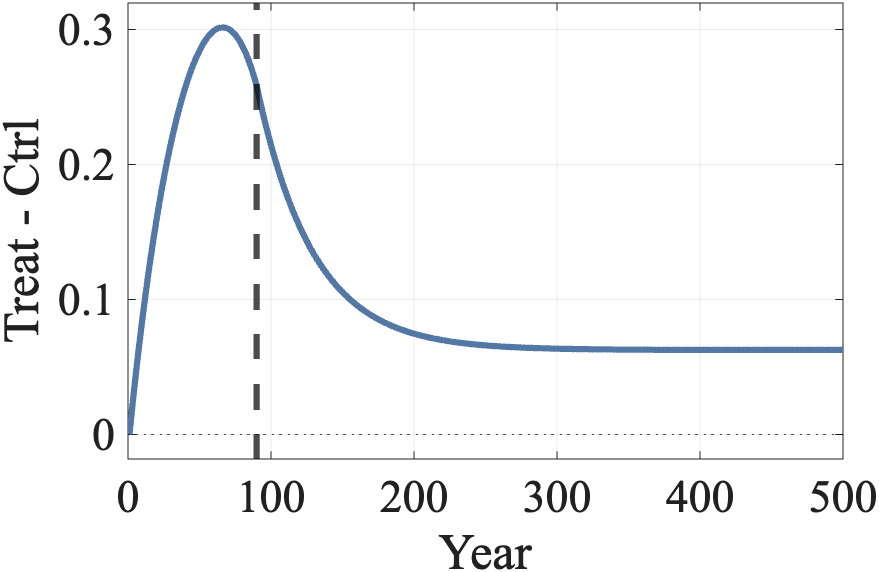
\includegraphics[width=\textwidth]{../Output/big_nu/graph_uncertainty_variance_shocks_no_migration_did/did_dynamic_moments_diff_wy.png}
  \end{minipage}
  \begin{minipage}{\textwidth}
  \vspace{0.5em}
  \footnotesize{\textbf{Note:} Difference-in-Differences (DiD) macro dynamic trajectories under Variance Shocks + No Migration autarky joint counterfactual. Metrics measure climate treatment differential $\Delta^{\text{DiD}} X_t = X_t^{\text{Treat}} - X_t^{\text{Ctrl}}$. Panel (a): annual earnings treatment diff $\Delta^{\text{DiD}} Y_t$. Panel (b): migration treatment diff $\Delta^{\text{DiD}} m_t \equiv 0$. Panel (c): total wealth treatment diff $\Delta^{\text{DiD}} W_t$. Panel (d): wealth-to-earnings ratio treatment diff $\Delta^{\text{DiD}} (W/Y)_t$.} \end{minipage}
  \label{fig:var_shock_1}
\end{figure}

% 2. Transition Maps (2x2)
\begin{figure}[H]
  \centering
  \caption{Transition Maps (Variance Shocks No Migration)}
  \begin{minipage}[t]{0.4\textwidth}
    \centering
    \small{(a) $\Delta$ Mean Welfare (CE)}
    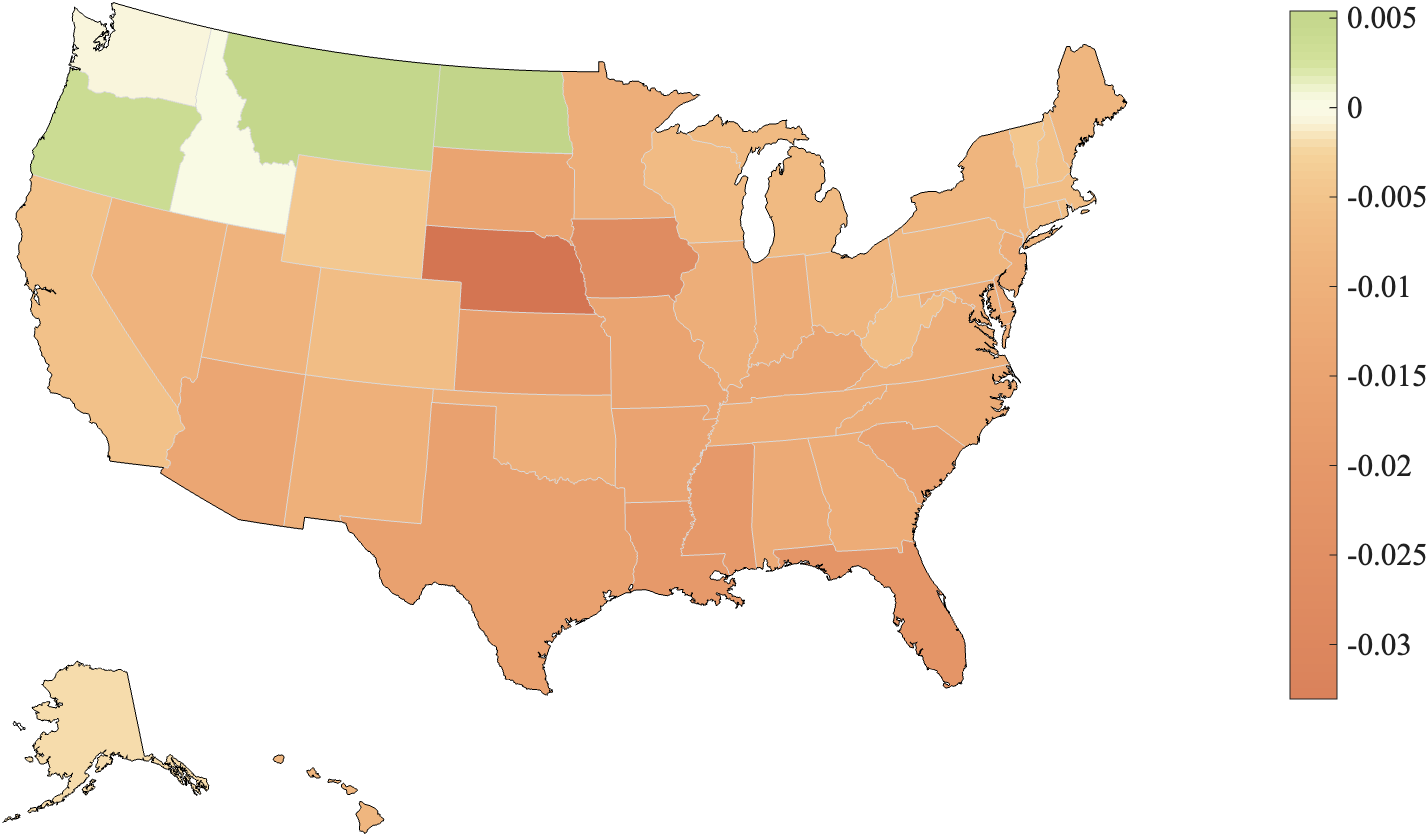
\includegraphics[width=\textwidth]{../Output/big_nu/graph_uncertainty_variance_shocks_no_migration_did/transition_maps/transition_maps_delta_mean_welfare_ce.png}
  \end{minipage}\hfill
  \begin{minipage}[t]{0.4\textwidth}
    \centering
    \small{(b) $\Delta$ W/Y Ratio in level}
    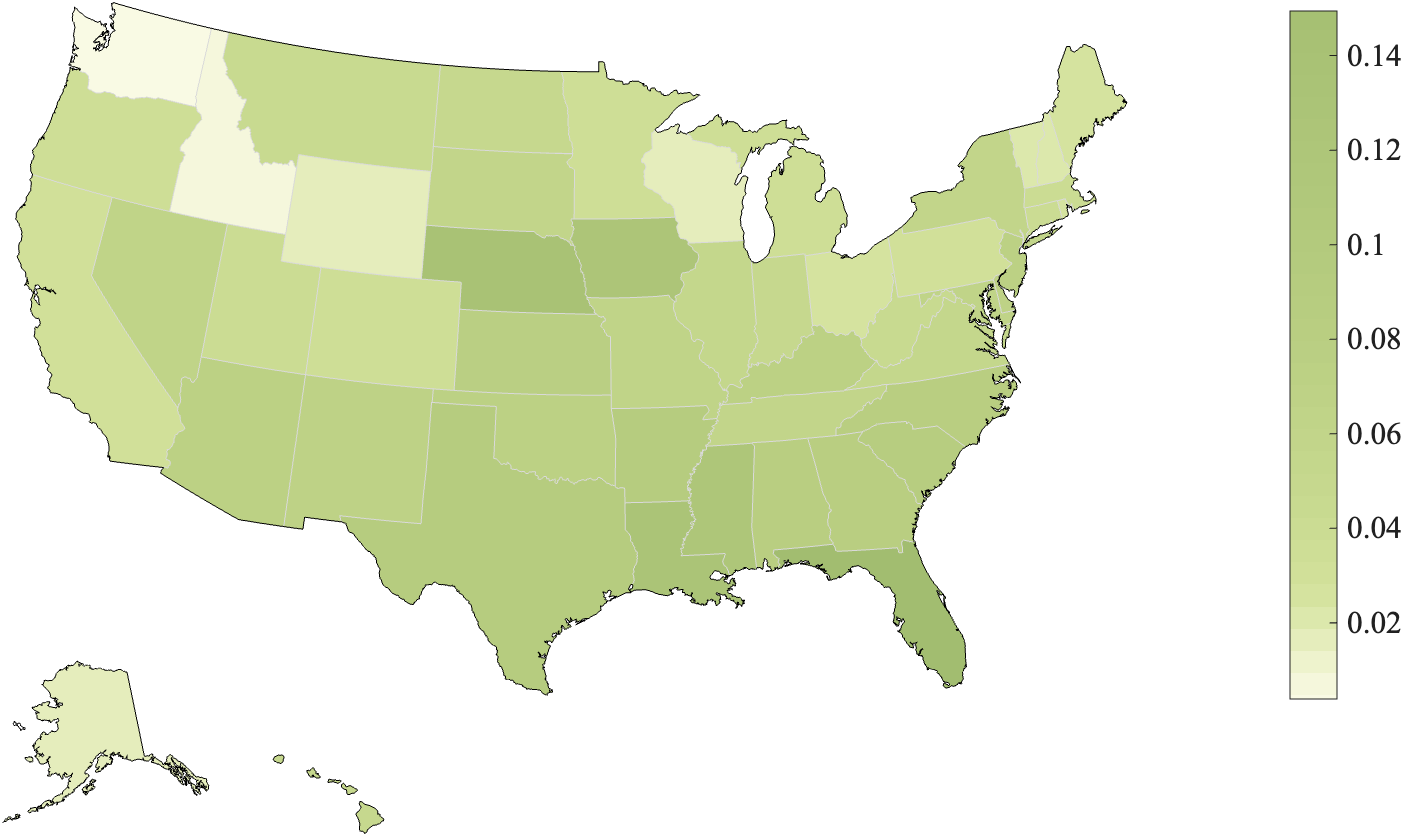
\includegraphics[width=\textwidth]{../Output/big_nu/graph_uncertainty_variance_shocks_no_migration_did/transition_maps/transition_maps_wealth_income_ratio_changes.png}
  \end{minipage}
  \vspace{1em}
  \begin{minipage}[t]{0.4\textwidth}
    \centering
    \small{(c) $\Delta$ Local Population (\%)}
    \includegraphics[width=\textwidth]{../Output/big_nu/graph_uncertainty_variance_shocks_no_migration_did/transition_maps/transition_maps_local_pop_changes_pct.png}
  \end{minipage}\hfill
  \begin{minipage}[t]{0.4\textwidth}
    \centering
    \small{(d) $\Delta$ Mean Wealth (\%)}
    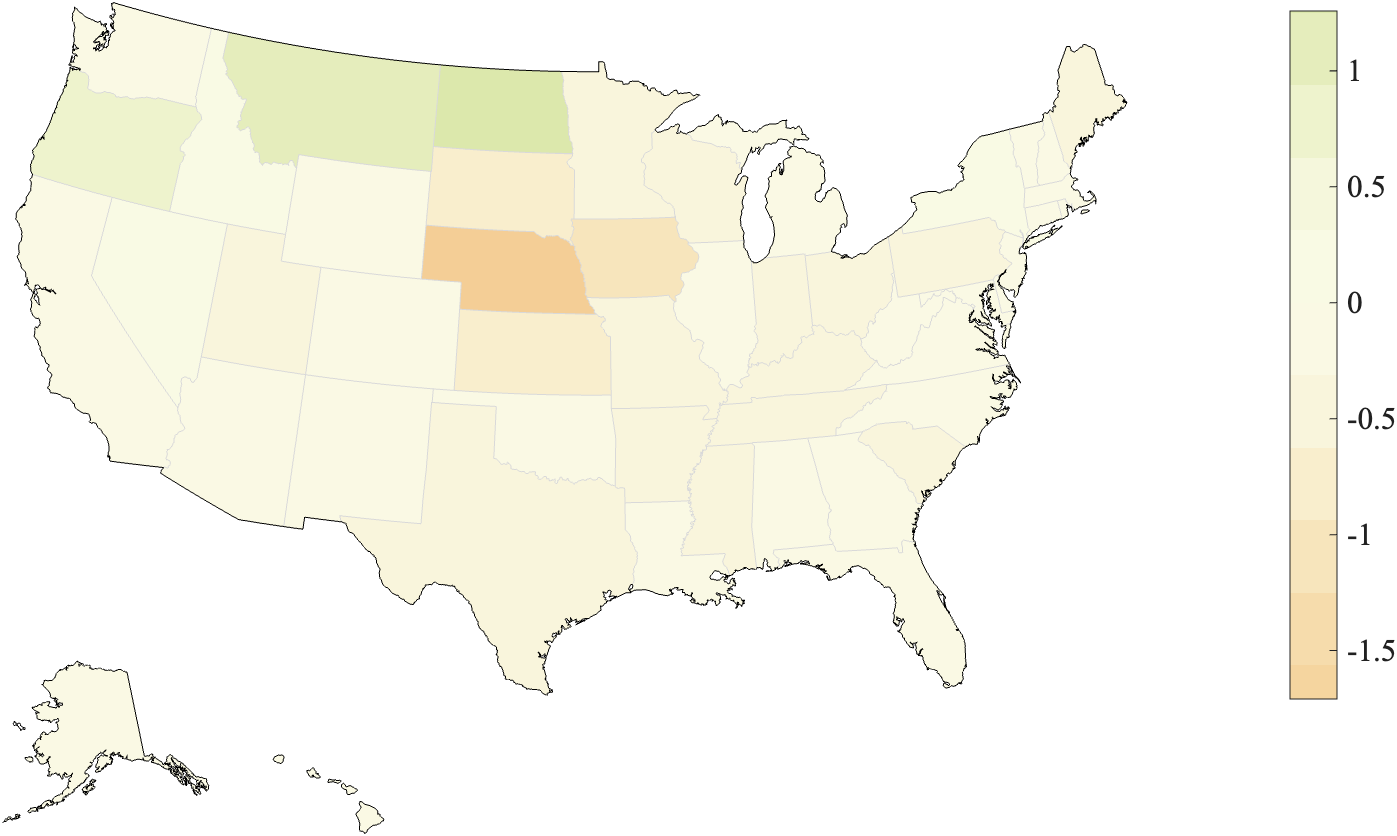
\includegraphics[width=\textwidth]{../Output/big_nu/graph_uncertainty_variance_shocks_no_migration_did/transition_maps/transition_maps_pop_changes_pp.png}
  \end{minipage}
  \begin{minipage}{\textwidth}
  \vspace{0.5em}
  \footnotesize{\textbf{Note:} Spatial maps comparing the terminal steady state under 2100 climate parameters ($SS_\text{term}$) to the initial 2010 baseline steady state ($SS_\text{init}$) under Variance Shocks + No Migration autarky. Panel (a): change in mean Certainty Equivalent welfare $\Delta \text{CE}_\ell = \overline{\text{CE}}_{\ell, \text{term}} - \overline{\text{CE}}_{\ell, \text{init}}$, showing massive welfare losses in high-variance states. Panel (b): change in state wealth-to-earnings ratio $\Delta (W/Y)_\ell = (W/Y)_{\ell, \text{term}} - (W/Y)_{\ell, \text{init}}$, capturing intense localized precautionary savings. Panel (c): relative population change $\Delta L_\ell\% \equiv 0$. Panel (d): percentage change in state mean per-capita wealth $\Delta \bar{a}_\ell\%$.} \end{minipage}
  \label{fig:var_shock_2}
\end{figure}

% 3. Welfare Inequality Maps only (1x2)
\begin{figure}[H]
  \centering
  \caption{Inequality Maps (Variance Shocks No Migration)}
  \begin{minipage}[t]{0.4\textwidth}
    \centering
    \small{(a) $\Delta$ Welfare Inequality (Std Dev \%)}
    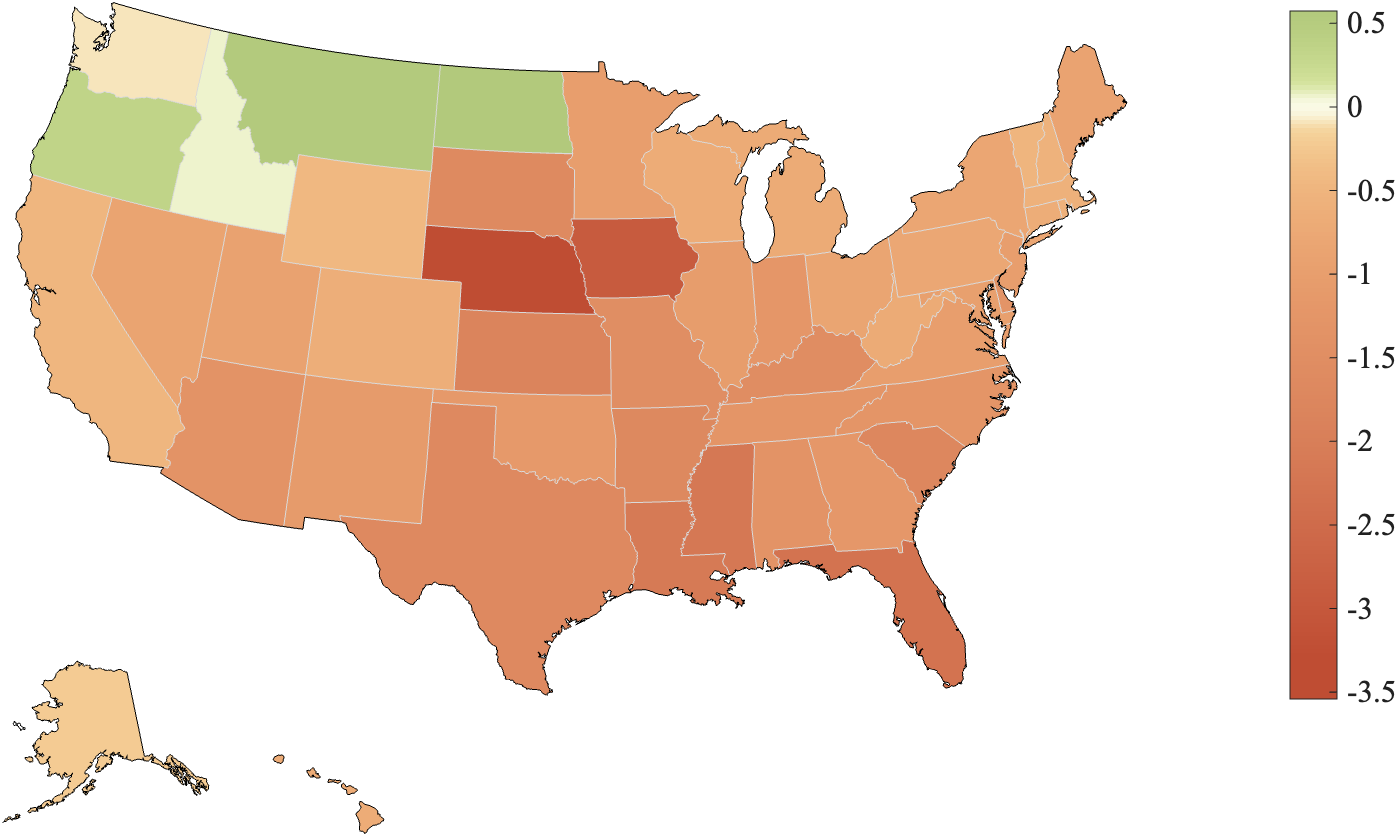
\includegraphics[width=\textwidth]{../Output/big_nu/graph_uncertainty_variance_shocks_no_migration_did/welfare_wealth_inequality_maps/welfare_wealth_inequality_maps_welfare_inequality.png}
  \end{minipage}\hfill
  \begin{minipage}[t]{0.4\textwidth}
    \centering
    \small{(b) $\Delta$ Wealth Inequality (Std Dev \%)}
    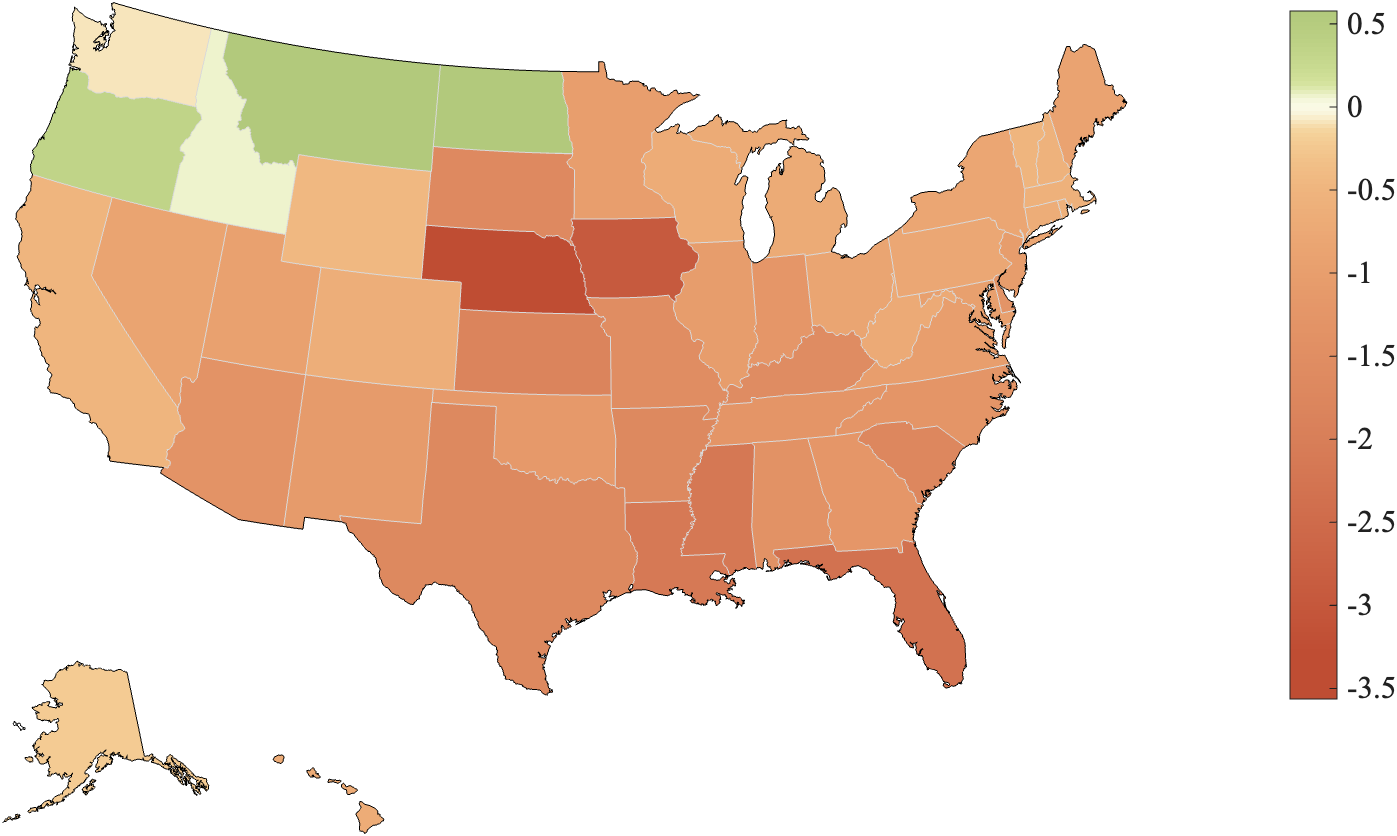
\includegraphics[width=\textwidth]{../Output/big_nu/graph_uncertainty_variance_shocks_no_migration_did/welfare_wealth_inequality_maps/welfare_wealth_inequality_maps_wealth_inequality.png}
  \end{minipage}
  \begin{minipage}{\textwidth}
  \vspace{0.5em}
  \footnotesize{\textbf{Note:} Spatial inequality maps under Variance Shocks + No Migration autarky. Panel (a): percentage change in the within-state welfare standard deviation $\text{Var}_z(\text{CE}_\ell(z)) = \frac{1}{L_\ell} \sum_z \Lambda(\ell,z) [\text{CE}_\ell(z) - \overline{\text{CE}}_\ell]^2$ between the two steady states. Panel (b): percentage change in the within-state wealth standard deviation $\text{Var}_z(\bar{a}_\ell(z)) = \frac{1}{L_\ell} \sum_z \Lambda(\ell,z) [\bar{a}_\ell(z) - \bar{a}_\ell]^2$ between the two steady states.} \end{minipage}
  \label{fig:var_shock_3}
\end{figure}

\subsection{Internally Calibrated $\nu$}
This section shows the model's results under the baseline scenario when the shape parameter of the Weibull distribution $\nu$ is calibrated internally to match an empirical target of 0.11 exhibited by \cite{dvorkin_geography_2025}. 

\begin{table}[!htb]
    \centering
    \caption{Parameters' values when $\nu$ is internally calibrated.}
    \label{tab:small_nu_params}
    \begin{tabular}{llcc}
        \toprule
        \textbf{Description} & \textbf{Parameter} & \textbf{Value} & \textbf{Calibration} \\
        \midrule
        Migration elasticity (Weibull shape) & $\nu$ & $2.1557$ & Internal \\
        Preference shock scale parameter & $\bar{\lambda}$ & $0.1631$ & Internal \\
        Fixed migration cost & $\psi_{\text{fix}}$ & $2.9911$ & Internal \\
        Distance elasticity & $\psi_{\text{dist}}$ & $0.7413$ & Internal \\
        Local amenities & $A_\ell$ &  From $-1.2417$ (D.C.) & Internal \\
        & & to $1.2417$ (California) & \\
        \bottomrule
    \end{tabular}
    
    \vspace{0.2cm}
    \begin{minipage}{0.9\textwidth}
        \small \textbf{Note:} This table reports the structural parameters of the model when $\nu$ is internally calibrated.
    \end{minipage}
\end{table}

\begin{figure}[!htb]
  \centering
  \caption{Dynamic Moments (Perfect Foresight)}
  \label{fig:trans_dyn_small_nu_pf}
  \begin{minipage}[t]{0.4\textwidth}
    \centering
    \small{(a) Earnings}
    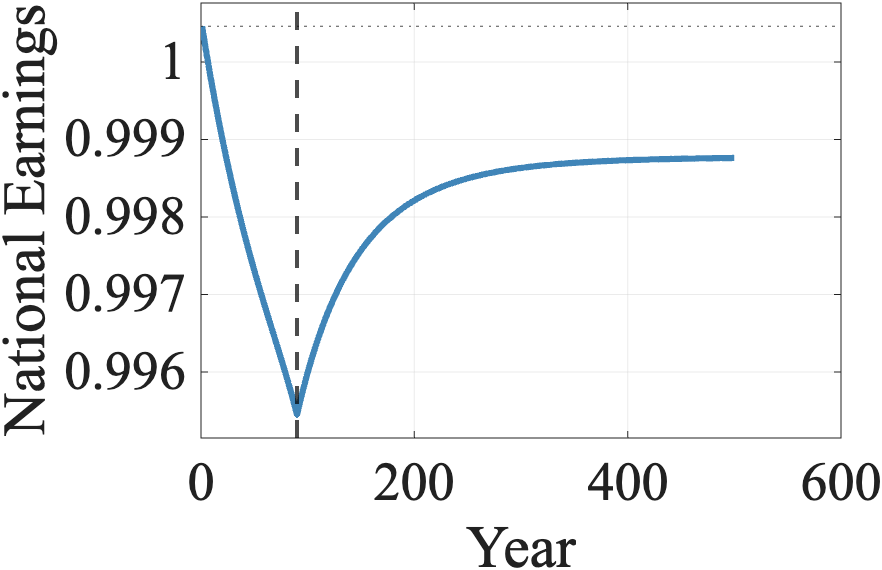
\includegraphics[width=\textwidth]{../Output/small_nu/graph_perfect_foresight/dynamic_moments/dynamic_moments_national_earnings.png}
  \end{minipage}\hfill
  \begin{minipage}[t]{0.4\textwidth}
    \centering
    \small{(b) Mobility}
    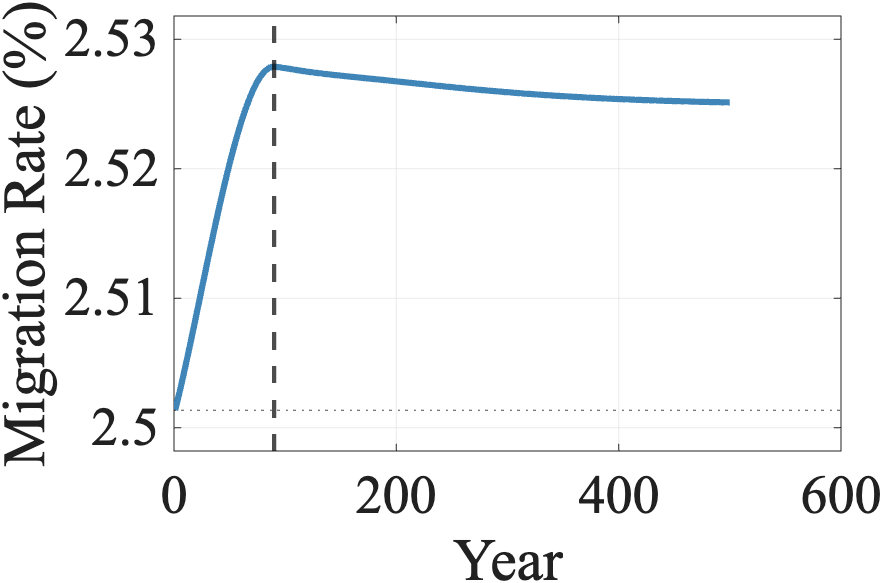
\includegraphics[width=\textwidth]{../Output/small_nu/graph_perfect_foresight/dynamic_moments/dynamic_moments_national_mobility.png}
  \end{minipage} \\[2ex]
  \begin{minipage}[t]{0.4\textwidth}
    \centering
    \small{(c) Wealth}
    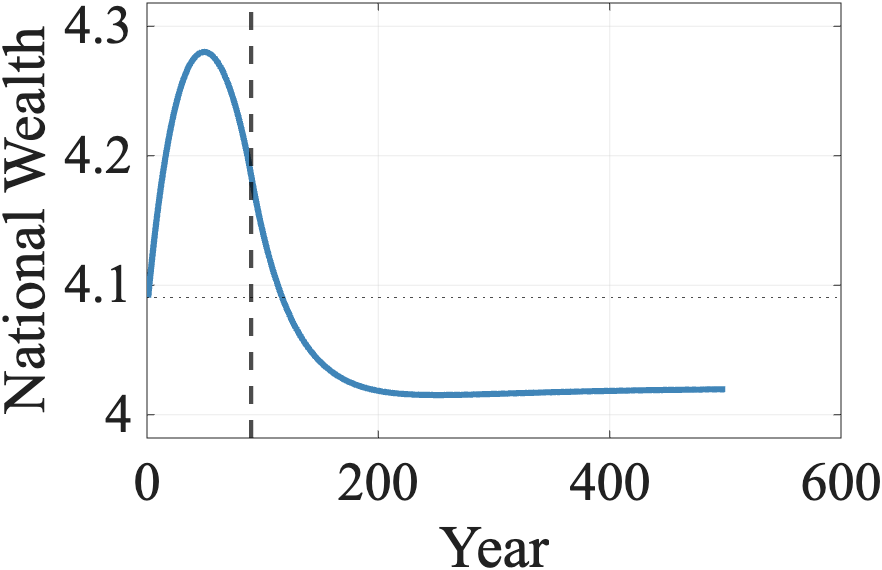
\includegraphics[width=\textwidth]{../Output/small_nu/graph_perfect_foresight/dynamic_moments/dynamic_moments_national_wealth.png}
  \end{minipage}\hfill
  \begin{minipage}[t]{0.4\textwidth}
    \centering
    \small{(d) W/Y Ratio}
    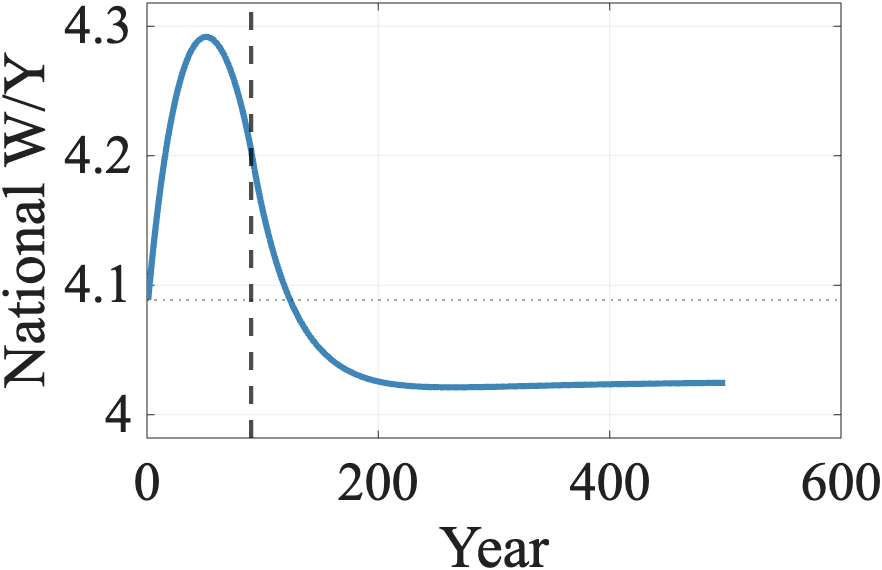
\includegraphics[width=\textwidth]{../Output/small_nu/graph_perfect_foresight/dynamic_moments/dynamic_moments_national_wy.png}
  \end{minipage} \begin{minipage}{\textwidth} 
  \vspace{0.5em}
  \footnotesize{\textbf{Note:} Aggregate macroeconomic time series under Perfect Foresight, 2010--2500+, with internal calibration of the Weibull shape parameter $\nu$.} \end{minipage}
\end{figure}

\begin{figure}[!htb]
  \centering
  \caption{Transition Maps (Perfect Foresight)}
  \label{fig:trans_map_small_nu_pf}
  \begin{minipage}[t]{0.4\textwidth}
    \centering
    \small{(a) $\Delta$ Mean Welfare (CE)}
    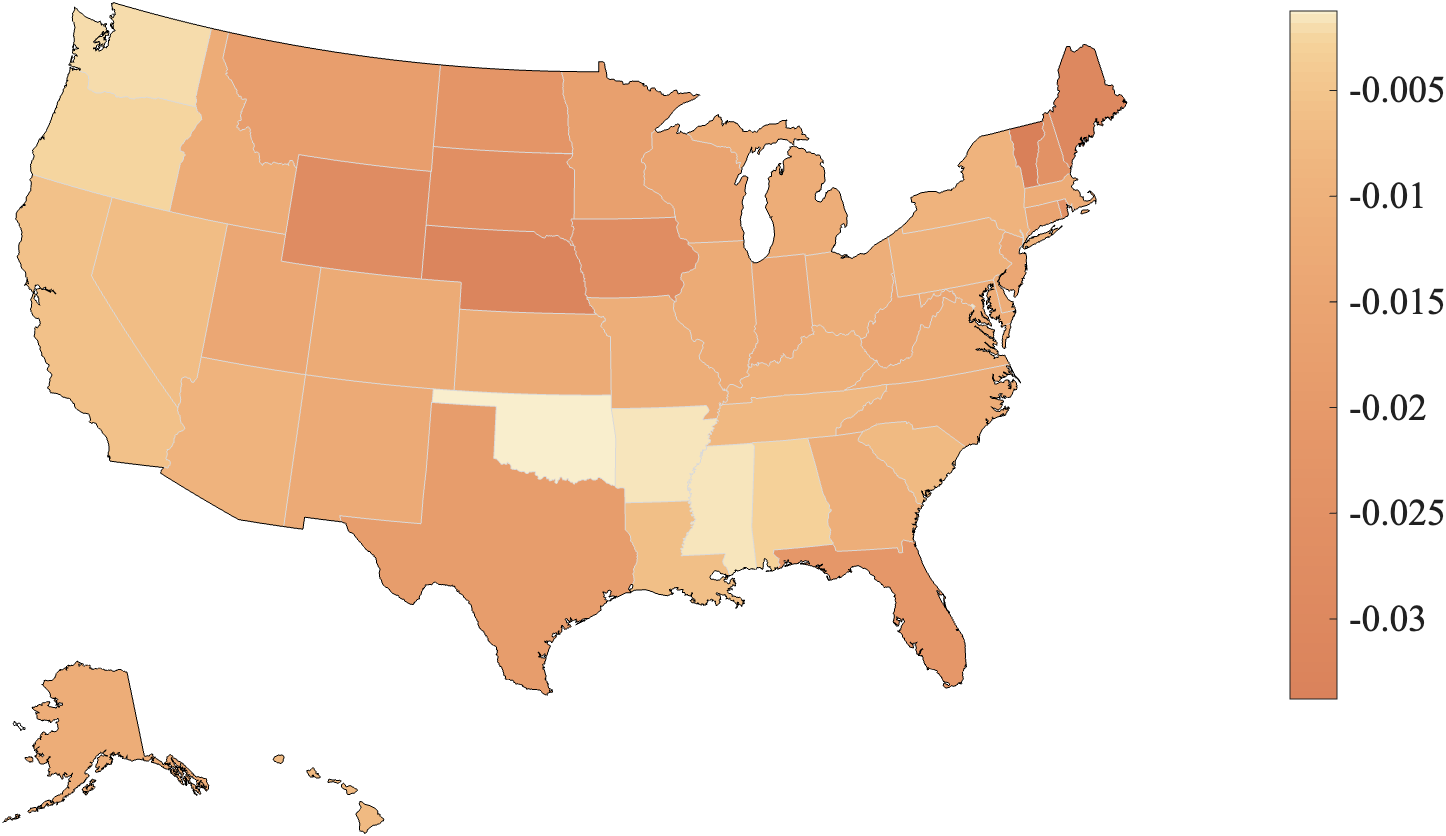
\includegraphics[width=\textwidth]{../Output/small_nu/graph_perfect_foresight/transition_maps/transition_maps_delta_mean_welfare_ce.png}
  \end{minipage}\hfill
  \begin{minipage}[t]{0.4\textwidth}
    \centering
    \small{(b) $\Delta$ W/Y Ratio in level}
    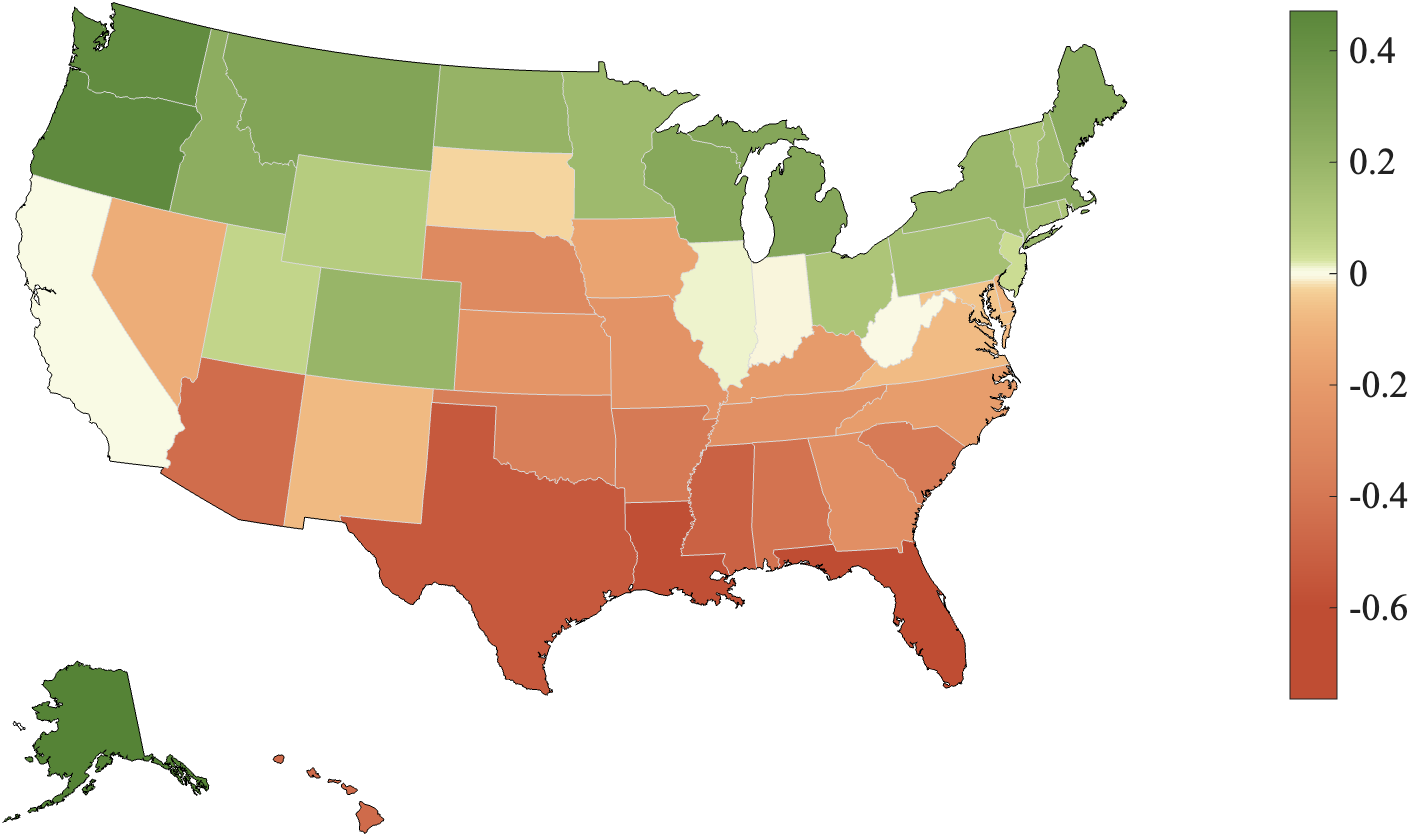
\includegraphics[width=\textwidth]{../Output/small_nu/graph_perfect_foresight/transition_maps/transition_maps_wealth_income_ratio_changes.png}
  \end{minipage}\\[2ex]
  \begin{minipage}[t]{0.4\textwidth}
    \centering
    \small{(c) $\Delta$ Local Population (\%)}
    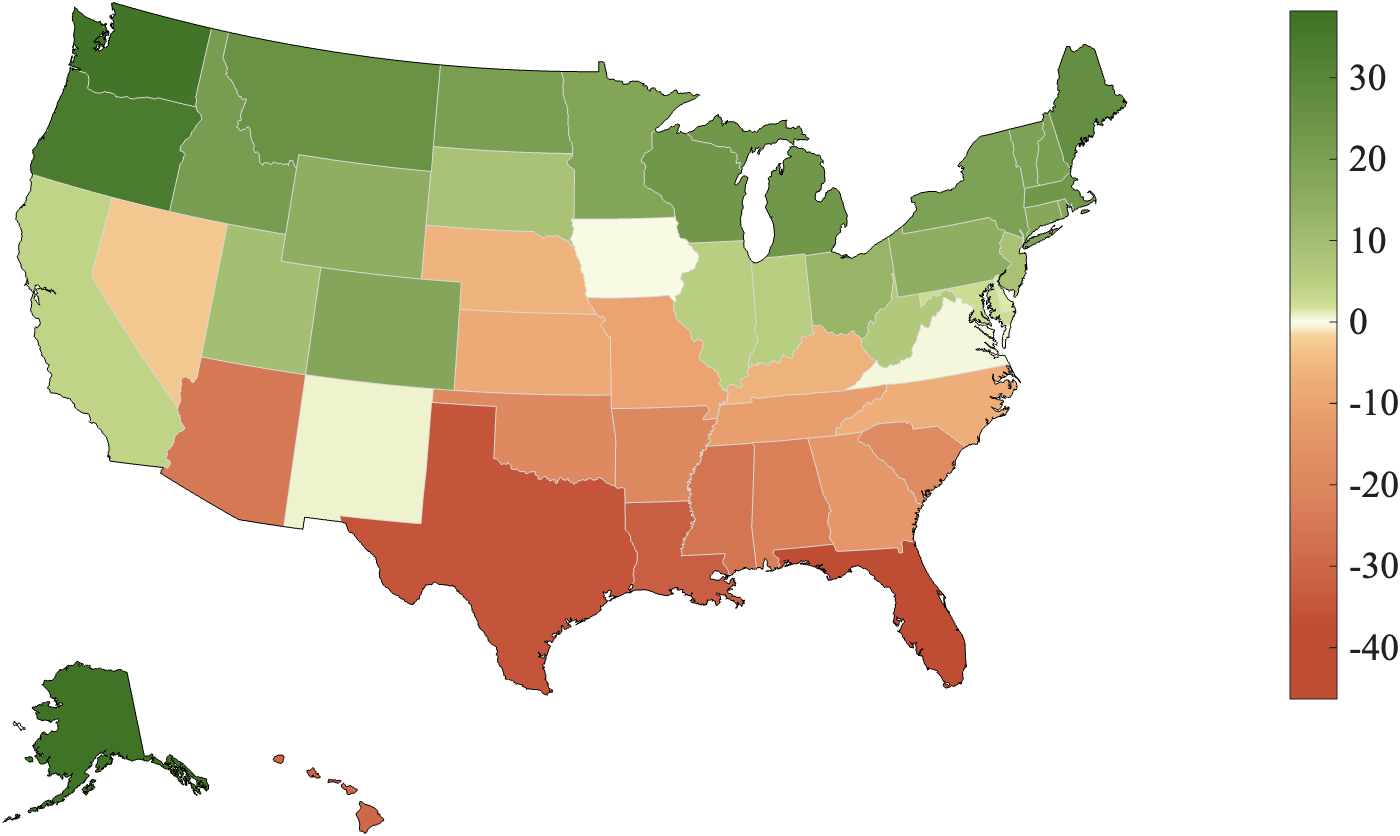
\includegraphics[width=\textwidth]{../Output/small_nu/graph_perfect_foresight/transition_maps/transition_maps_local_pop_changes_pct.png}
  \end{minipage}\hfill
  \begin{minipage}[t]{0.4\textwidth}
    \centering
    \small{(d) $\Delta$ Mean Wealth (\%)}
    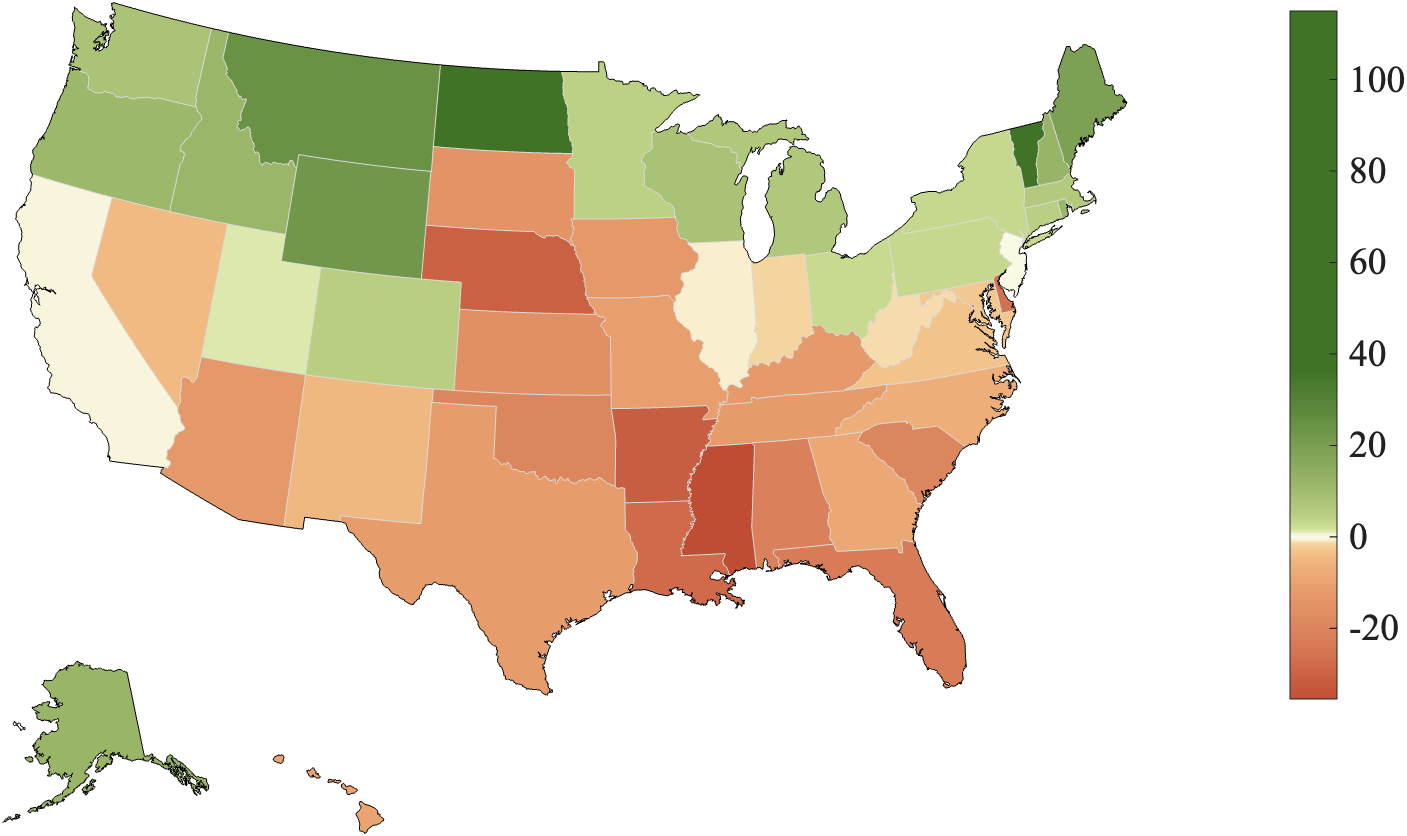
\includegraphics[width=\textwidth]{../Output/small_nu/graph_perfect_foresight/transition_maps/transition_maps_pop_changes_pp.png}
  \end{minipage}
   \begin{minipage}{\textwidth}
  \vspace{0.5em}
  \footnotesize{\textbf{Note:} Spatial maps comparing the terminal steady state under 2100 climate parameters ($SS_\text{term}$) to the initial 2010 baseline steady state ($SS_\text{init}$) under Perfect Foresight with internal calibration of the Weibull shape parameter $\nu$}. \end{minipage}
\end{figure}

\begin{figure}[!htb]
  \centering
    \caption{Wealth's Change Decomposition (Perfect Foresight)}
  \label{fig:trans_wy_small_nu}
  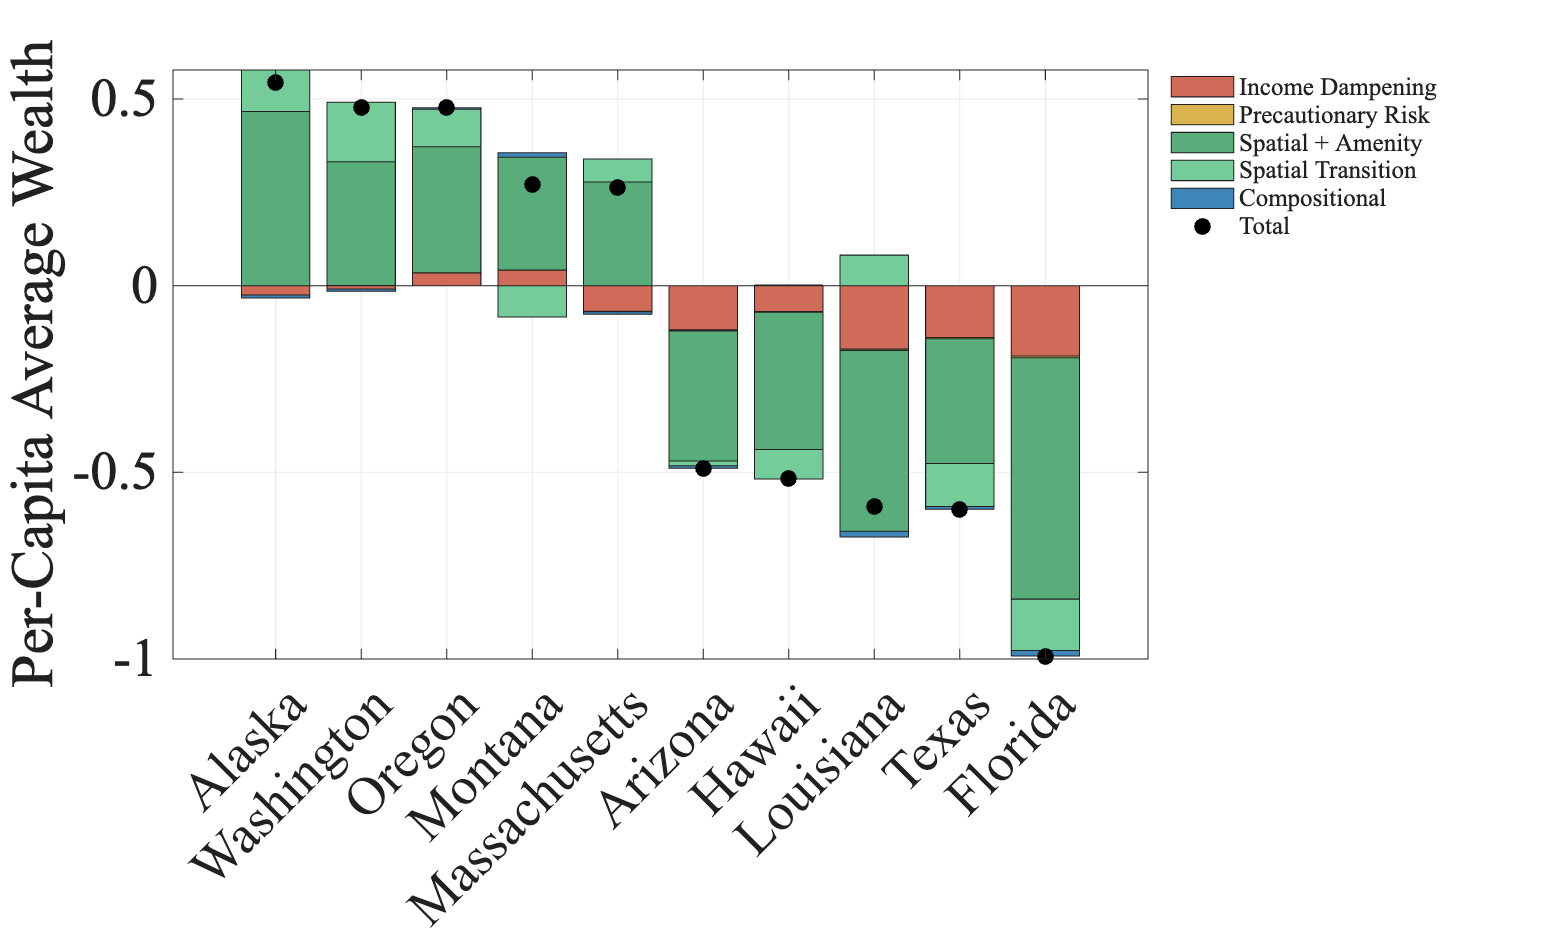
\includegraphics[width=\textwidth]{../Output/small_nu/graph_perfect_foresight/exact_percapita_decomposition_bar_no_counterfactual_no_counterfactual.png}
  \begin{minipage}{\textwidth}
  \vspace{0.5em}
  \footnotesize{\textbf{Note:} Structural shift-share decomposition of the state-level per-capita wealth change $\Delta \bar{a}_\ell = \bar{a}_{\ell, \text{term}} - \bar{a}_{\ell, \text{init}}$ under Perfect Foresight with internal calibration of the Weibull shape parameter $\nu$.} \end{minipage}
\end{figure}


\section{Summary Tables}
\label{sec:summary}
\begin{table}[H]
    \centering
    \footnotesize
    \renewcommand{\arraystretch}{0.85}
    \caption{State-Specific Income Process Parameters}
    \label{tab:state_income_process}
    \begin{tabular}{lcc}
        \toprule
        \textbf{State} & \textbf{Persistent Variance} ($\sigma_{\epsilon,\ell}^2$) & \textbf{Transitory Variance} ($\sigma_{\eta,\ell}^2$) \\
        \midrule
        Alabama & 0.0110 & 0.0980 \\
        Alaska & 0.0140 & 0.1080 \\
        Arizona & 0.0150 & 0.0920 \\
        Arkansas & 0.0130 & 0.0940 \\
        California & 0.0210 & 0.1000 \\
        Colorado & 0.0180 & 0.0940 \\
        Connecticut & 0.0170 & 0.0930 \\
        Delaware & 0.0130 & 0.0910 \\
        District of Columbia & 0.0230 & 0.0890 \\
        Florida & 0.0150 & 0.1110 \\
        Georgia & 0.0150 & 0.1090 \\
        Hawaii & 0.0160 & 0.1090 \\
        Idaho & 0.0170 & 0.0730 \\
        Illinois & 0.0200 & 0.0900 \\
        Indiana & 0.0150 & 0.0750 \\
        Iowa & 0.0150 & 0.0770 \\
        Kansas & 0.0180 & 0.0760 \\
        Kentucky & 0.0150 & 0.0830 \\
        Louisiana & 0.0160 & 0.1000 \\
        Maine & 0.0170 & 0.0620 \\
        Maryland & 0.0200 & 0.0990 \\
        Massachusetts & 0.0170 & 0.1070 \\
        Michigan & 0.0140 & 0.0860 \\
        Minnesota & 0.0170 & 0.0660 \\
        Mississippi & 0.0140 & 0.0940 \\
        Missouri & 0.0160 & 0.0780 \\
        Montana & 0.0150 & 0.0800 \\
        Nebraska & 0.0150 & 0.0660 \\
        Nevada & 0.0140 & 0.1120 \\
        New Hampshire & 0.0190 & 0.0700 \\
        New Jersey & 0.0230 & 0.1080 \\
        New Mexico & 0.0170 & 0.1020 \\
        New York & 0.0190 & 0.1120 \\
        North Carolina & 0.0150 & 0.1060 \\
        North Dakota & 0.0130 & 0.0730 \\
        Ohio & 0.0160 & 0.0640 \\
        Oklahoma & 0.0140 & 0.1030 \\
        Oregon & 0.0170 & 0.0750 \\
        Pennsylvania & 0.0180 & 0.0730 \\
        Rhode Island & 0.0150 & 0.0770 \\
        South Carolina & 0.0140 & 0.0870 \\
        South Dakota & 0.0130 & 0.0670 \\
        Tennessee & 0.0170 & 0.0830 \\
        Texas & 0.0180 & 0.0930 \\
        Utah & 0.0170 & 0.0790 \\
        Vermont & 0.0140 & 0.0750 \\
        Virginia & 0.0210 & 0.0910 \\
        Washington & 0.0210 & 0.0700 \\
        West Virginia & 0.0130 & 0.0990 \\
        Wisconsin & 0.0160 & 0.0520 \\
        Wyoming & 0.0110 & 0.0750 \\
        \bottomrule
    \end{tabular}
\end{table}

\begin{table}[H]
    \centering
    \footnotesize
    \renewcommand{\arraystretch}{0.85}
    \caption{Wages, Amenities, Wealth, and Housing Cost by State (Initial Steady State)}
    \label{tab:state_wages_amenities_wealth}
    \begin{tabular}{lcccc}
        \toprule
        \textbf{State} & \textbf{Base Wage} ($w_\ell$) & \textbf{Amenity} ($A_\ell$) & \textbf{Mean Wealth} ($W_{2010}$) & \textbf{Housing Cost} ($q_\ell$) \\
        \midrule
        Alabama & 0.9133 & -0.0719 & 2.5339 & 0.1777 \\
        Alaska & 1.1131 & -0.2356 & 4.8188 & 0.3436 \\
        Arizona & 0.9762 & 0.2482 & 3.8989 & 0.2813 \\
        Arkansas & 0.8893 & -0.1617 & 2.0065 & 0.1781 \\
        California & 1.0932 & 0.9019 & 6.5662 & 0.4741 \\
        Colorado & 1.0262 & 0.3112 & 3.9108 & 0.3716 \\
        Connecticut & 1.1241 & -0.0063 & 4.2522 & 0.3974 \\
        Delaware & 1.0042 & -0.5975 & 2.1063 & 0.2855 \\
        District of Columbia & 1.2081 & -0.6123 & 3.0741 & 0.5351 \\
        Florida & 0.9413 & 0.6755 & 4.1439 & 0.3278 \\
        Georgia & 0.9513 & 0.2244 & 3.4810 & 0.2414 \\
        Hawaii & 1.0462 & 0.4887 & 5.2336 & 0.4612 \\
        Idaho & 0.9213 & -0.1664 & 2.3937 & 0.2226 \\
        Illinois & 1.0202 & 0.2964 & 4.1519 & 0.3099 \\
        Indiana & 0.9403 & 0.0523 & 2.8481 & 0.2213 \\
        Iowa & 0.9283 & -0.1466 & 2.3246 & 0.2101 \\
        Kansas & 0.9303 & -0.1096 & 2.3743 & 0.2252 \\
        Kentucky & 0.9093 & -0.0562 & 2.3009 & 0.1988 \\
        Louisiana & 0.9343 & 0.0003 & 2.8066 & 0.2145 \\
        Maine & 0.9333 & -0.2902 & 2.1248 & 0.2311 \\
        Maryland & 1.1241 & 0.1067 & 4.5578 & 0.3945 \\
        Massachusetts & 1.1211 & 0.1744 & 4.8976 & 0.3900 \\
        Michigan & 0.9722 & 0.1617 & 3.5828 & 0.2422 \\
        Minnesota & 1.0502 & -0.0087 & 3.9610 & 0.2917 \\
        Mississippi & 0.8933 & -0.1698 & 2.0648 & 0.1758 \\
        Missouri & 0.9553 & 0.0024 & 2.9890 & 0.2197 \\
        Montana & 0.9013 & -0.2886 & 1.9010 & 0.2215 \\
        Nebraska & 0.9333 & -0.2455 & 2.1482 & 0.2262 \\
        Nevada & 1.0052 & 0.0224 & 3.6135 & 0.2962 \\
        New Hampshire & 1.0322 & -0.2145 & 2.7107 & 0.3590 \\
        New Jersey & 1.1231 & 0.3553 & 5.0190 & 0.4358 \\
        New Mexico & 0.9483 & -0.1604 & 2.5931 & 0.2365 \\
        New York & 1.0542 & 0.6095 & 5.0313 & 0.4030 \\
        North Carolina & 0.9463 & 0.1814 & 3.3470 & 0.2273 \\
        North Dakota & 0.9503 & -0.5701 & 1.8537 & 0.2342 \\
        Ohio & 0.9563 & 0.1719 & 3.4207 & 0.2267 \\
        Oklahoma & 0.9063 & -0.0367 & 2.4081 & 0.1991 \\
        Oregon & 1.0212 & 0.1484 & 4.1304 & 0.3161 \\
        Pennsylvania & 0.9892 & 0.2440 & 3.8763 & 0.2668 \\
        Rhode Island & 1.0362 & -0.3966 & 2.5395 & 0.3394 \\
        South Carolina & 0.9143 & 0.0635 & 2.5417 & 0.2237 \\
        South Dakota & 0.8933 & -0.5632 & 1.4708 & 0.1865 \\
        Tennessee & 0.8953 & 0.1587 & 2.5030 & 0.2183 \\
        Texas & 0.9513 & 0.5702 & 4.4759 & 0.2819 \\
        Utah & 0.9732 & 0.0311 & 3.1221 & 0.2809 \\
        Vermont & 0.9463 & -0.5425 & 1.6446 & 0.2967 \\
        Virginia & 1.0552 & 0.2129 & 4.1508 & 0.3446 \\
        Washington & 1.1051 & 0.2129 & 5.5138 & 0.3588 \\
        West Virginia & 0.8863 & -0.3431 & 1.6283 & 0.1851 \\
        Wisconsin & 0.9693 & 0.0364 & 3.1280 & 0.2436 \\
        Wyoming & 0.9633 & -0.6687 & 1.8486 & 0.2498 \\
        \bottomrule
    \end{tabular}
\end{table}

\begin{table}[H]
    \centering
    \footnotesize
    \renewcommand{\arraystretch}{0.85}
    \caption{Wages, Amenities, and Housing Cost by State (Terminal Steady State)}
    \label{tab:state_wages_amenities_housing_terminal}
    \begin{tabular}{lccc}
        \toprule
        \textbf{State} & \textbf{Terminal Wage} ($w_\ell$) & \textbf{Terminal Amenity} ($A_\ell$) & \textbf{Terminal Housing Cost} ($q_\ell$) \\
        \midrule
        Alabama & 0.9008 & -0.2245 & 0.1784 \\
        Alaska & 1.1107 & -0.1317 & 0.3435 \\
        Arizona & 0.9630 & 0.1024 & 0.2823 \\
        Arkansas & 0.8743 & -0.3068 & 0.1788 \\
        California & 1.0878 & 0.8538 & 0.4745 \\
        Colorado & 1.0197 & 0.3354 & 0.3719 \\
        Connecticut & 1.1168 & 0.0211 & 0.3975 \\
        Delaware & 0.9912 & -0.6396 & 0.2861 \\
        District of Columbia & 1.1960 & -0.7003 & 0.5358 \\
        Florida & 0.9194 & 0.4412 & 0.3287 \\
        Georgia & 0.9397 & 0.1277 & 0.2420 \\
        Hawaii & 1.0390 & 0.3253 & 0.4624 \\
        Idaho & 0.9219 & -0.1306 & 0.2228 \\
        Illinois & 1.0095 & 0.2724 & 0.3104 \\
        Indiana & 0.9288 & 0.0332 & 0.2218 \\
        Iowa & 0.9009 & -0.1524 & 0.2105 \\
        Kansas & 0.9131 & -0.1851 & 0.2257 \\
        Kentucky & 0.8953 & -0.1286 & 0.1994 \\
        Louisiana & 0.9143 & -0.1824 & 0.2151 \\
        Maine & 0.9249 & -0.1853 & 0.2312 \\
        Maryland & 1.1133 & 0.0683 & 0.3953 \\
        Massachusetts & 1.1146 & 0.2170 & 0.3901 \\
        Michigan & 0.9653 & 0.2029 & 0.2427 \\
        Minnesota & 1.0394 & 0.0267 & 0.2922 \\
        Mississippi & 0.8738 & -0.3409 & 0.1764 \\
        Missouri & 0.9407 & -0.0836 & 0.2203 \\
        Montana & 0.9064 & -0.2213 & 0.2216 \\
        Nebraska & 0.8941 & -0.2637 & 0.2267 \\
        Nevada & 0.9966 & -0.0483 & 0.2970 \\
        New Hampshire & 1.0266 & -0.1483 & 0.3590 \\
        New Jersey & 1.1115 & 0.3473 & 0.4365 \\
        New Mexico & 0.9379 & -0.1991 & 0.2370 \\
        New York & 1.0457 & 0.6254 & 0.4035 \\
        North Carolina & 0.9342 & 0.1080 & 0.2279 \\
        North Dakota & 0.9558 & -0.5051 & 0.2345 \\
        Ohio & 0.9482 & 0.1730 & 0.2273 \\
        Oklahoma & 0.8959 & -0.1809 & 0.1998 \\
        Oregon & 1.0249 & 0.2077 & 0.3162 \\
        Pennsylvania & 0.9814 & 0.2494 & 0.2673 \\
        Rhode Island & 1.0301 & -0.3422 & 0.3395 \\
        South Carolina & 0.8983 & -0.0624 & 0.2243 \\
        South Dakota & 0.8785 & -0.5370 & 0.1868 \\
        Tennessee & 0.8839 & 0.0610 & 0.2189 \\
        Texas & 0.9353 & 0.4182 & 0.2827 \\
        Utah & 0.9642 & 0.0271 & 0.2813 \\
        Vermont & 0.9415 & -0.4505 & 0.2968 \\
        Virginia & 1.0444 & 0.1668 & 0.3452 \\
        Washington & 1.1043 & 0.2754 & 0.3587 \\
        West Virginia & 0.8799 & -0.3566 & 0.1855 \\
        Wisconsin & 0.9626 & 0.0871 & 0.2439 \\
        Wyoming & 0.9589 & -0.6140 & 0.2499 \\
        \bottomrule
    \end{tabular}
\end{table}

\begin{table}[H]
\centering
\small
\renewcommand{\arraystretch}{1.3}
\begin{tabular}{>{\raggedright}p{3.2cm}
                >{\raggedright}p{5.0cm}
                >{\raggedright\arraybackslash}p{5.4cm}}
\toprule
\textbf{Step} & \textbf{Dvorkin \& Greaney} & \textbf{My approach} \\
\midrule
Income process & Re-estimated with spatial selection correction
               & Baseline taken from Table 9 \\
\addlinespace
Parameters & Re-estimated from microdata
                & Calibrated via Moments matching \\
\addlinespace
Moving cost spec. & Residual with the amenities
                  & Two-parameter: $\psi_{\text{fixed}} + \psi_{\text{dist}} \cdot \log(1 + d_{j\ell})$ \\
\addlinespace
Outer calibration & Analytic identification from log-mobility differences
                  & \texttt{fsolve} (Gradient ascent) on 3 moments: mobility rate, avg.\ log-distance, $W/Y$ ratio \\
\addlinespace
Amenity identification & Residual with the migration costs
                       & Contraction mapping on population share residuals \\
\addlinespace
Stationary distribution & --- & Matrix inversion $(I-T)^{-1}$, no iterative loop \\
\addlinespace
Equilibrium concept & Stationary (two SS compared)
                    & Transition path + sequence of equilibria \\
\addlinespace
Dynamics & None (two SS)
         & Backward VFI over time-varying wage path \\
\addlinespace
Climate & Not modelled
        & Exogenous $(w_{\ell,t}, A_{\ell,t}, q_{\ell,t})$ and $\sigma^2_{\varepsilon,t}$  \\
\addlinespace
Geographic scale & 51 US states
                 & 51 US states\\
\bottomrule
\end{tabular}
\caption{Comparison of the Dvorkin \& Greaney (2025) strategy and the proposed thesis extensions.}
\label{tab:comparison}
\end{table}

% ---------------------------------------------------------
% DATA SECTION APPENDIX
% ------------------------------------------------------
\section{Data description}
\label{app:data}

\paragraph{IRS State-to-State Migration} Derived from the Internal Revenue Service (IRS) Statistics of Income (SOI) Division State-to-State Migration Data for Tax Years 2015--2016 \citep{irs2016migration}. The dataset represents administrative longitudinal tracking of U.S. household location choices, capturing approximately 95\%--98\% of tax-filing units by matching Social Security Numbers (SSNs) across consecutive calendar years 2015 and 2016.

%\paragraph{USDA Natural Amenities Scale} Compiled from the USDA Economic Research Service (ERS) Natural Amenities Scale \citep{mcgranahan1999natural}. The scale combines six physical environmental attributes across 3,111 contiguous U.S. counties: (1) mean January temperature, (2) mean January hours of sunlight, (3) low July relative humidity, (4) low July heat moderation relative to January, (5) topographic variation code, and (6) log surface water area share. County natural amenity scores ($\text{nat\_amenity\_scale}_c \in \{1,\dots,7\}$) are joined with 1990 Decennial Census county population counts (\texttt{cencounts.csv}). The state-level natural amenity score is calculated as a population-weighted average:
%\begin{equation}
%\label{eq:pop_weighted_amenity}
%\text{pop\_weighted\_amenity}_s = \frac{\sum_{c \in \mathcal{C}_s} \text{nat\_amenity\_scale}_c \cdot \text{pop1990}_c}{\sum_{c \in \mathcal{C}_s} \text{pop1990}_c}
%\end{equation}
%where $\mathcal{C}_s$ denotes the set of counties in state $s$, and $\text{pop1990}_c$ is county population in 1990.


%\paragraph{NAEP Educational Performance Index.} Obtained from the National Centre for Education Statistics (NCES), Institute of Education Sciences, U.S. Department of Education \citep{nces2015naep}. The National Assessment of Educational Progress (NAEP), \textit{The Nation's Report Card}, provides representative public school student achievement scores for Grade 8 Mathematics and Grade 8 Reading. To isolate institutional public school quality from student socioeconomic background, the pipeline filters explicitly for students designated as \textbf{"Not eligible"} for the National School Lunch Program (NSLP). For both subjects, average scale scores $\bar{y}_{s,\text{math}}$ and $\bar{y}_{s,\text{reading}}$ are standardised across the 51 locations into z-scores:
% \begin{align}
%\label{eq:naep_z_scores}
%\text{math\_z}_s &= \frac{\bar{y}_{s,\text{math}} - \mu_{\text{math}}}%{\sigma_{\text{math}}}, \quad \text{reading\_z}_s = \frac{\bar{y}_{s,\text{reading}} - \mu_{\text{reading}}}{\sigma_{\text{reading}}} \\[6pt]
%\label{eq:edu_amenity_index}
%u_{\text{edu}, s} &= \frac{\text{math\_z}_s + \text{reading\_z}_s}{2}
%\end{align}


%\paragraph{Fraser Institute Economic Freedom Index.} Institutional policy quality is measured using the Fraser Institute Economic Freedom of North America (EFNA) subnational index \citep{stansel2020economic, stansel2013economic}, which evaluates government spending, tax productivity, and labour market freedom (0--10 scale). Annual scores from 2005 to 2010 (\texttt{EconFreedom.csv}) are averaged by state and standardised to $u_{\text{freedom}, s}$. 

\paragraph{BEA Agricultural Share.} Agricultural sectoral exposure $s_{\text{agri}, s}$ is derived from the Bureau of Economic Analysis (BEA) Regional Economic Accounts (SAGDP2 Gross Domestic Product by State) \citep{bea2015sagdp} by taking the 2010--2015 average ratio of Agricultural GDP (\texttt{LineCode == 3}) to Total GDP (\texttt{LineCode == 1}).

\paragraph{FBI Uniform Crime Reporting Statistics.} Derived from the Federal Bureau of Investigation (FBI) Uniform Crime Reporting (UCR) Program \citep{fbi2015ucr}. Annual violent crime rates (homicide, rape, robbery, aggravated assault) and property crime rates (burglary, larceny-theft, motor vehicle theft) per 100,000 residents are averaged over 2010--2015 \citep{mccollister_cost_2010}. The baseline safety amenity score $u_{\text{crime}, s}$ is constructed as the inverse z-score of state violent crime rates.

%\paragraph{Census CBP Urban Consumption Variety } Compiled from the U.S. Census Bureau County Business Patterns (CBP) 2015 dataset \citep{census2015cbp}. The CBP dataset provides administrative annual establishment counts and employment figures by subnational geographic unit and North American Industry Classification System (NAICS) industry codes. To capture local urban consumption variety and service-sector amenity availability, I filter establishment counts for two key consumer service sectors: NAICS 71 (Arts, Entertainment, and Recreation) and NAICS 72 (Accommodation and Food Services). The raw state-level variety share $s_{\text{variety}, s}$ is computed relative to total state establishments $N_{s, \text{NAICS 00}}$:


%\paragraph{Census Experienced Population-Weighted Density.} Retrieved from the U.S. Census Bureau 2010 Decennial Census tract-level population counts and land area geometries \citep{census2010decennial, census2015cbp}. To avoid distortions caused by vast uninhabited land areas in Western states, I compute \textit{population-weighted experienced tract density} :

\paragraph{CPS Outgoing Rotation Group (CPS-ORG).} To anchor the model's nominal values and calculate the national average annual income ($\bar{Y}_{\text{US}}$) required to monetise utility-equivalent amenity shocks, I use microdata from the Current Population Survey Outgoing Rotation Group (CPS-ORG) spanning 2010 to 2015. The sample is restricted to prime-age employed individuals (aged 25--60) with valid weekly earnings (\texttt{EARNWEEK2}). After trimming the top and bottom 1 per cent of the weekly earnings distribution to remove outliers, the national average weekly earnings are computed using the official CPS earnings weights (\texttt{EARNWT}) and annualised to obtain the national aggregate $\bar{Y}_{\text{US}}$.

\paragraph{BEA State Personal Income and Energy Expenditures.} To construct the housing cost shock channel ($D^q_{\ell, t}$), which primarily captures the direct effect of climate change on energy demand, I utilise state-level data from the Bureau of Economic Analysis (BEA) Regional Economic Accounts. I compute the baseline energy expenditure share for each state by taking the ratio of total residential electricity expenditures to total state personal income for the year 2010. This state-specific energy share is then interacted with the county-level projected percentage changes in energy expenditures from \citet{hsiang_estimating_2017} to calculate the effective housing cost shock for each location.

\bibliographystyle{plainnat}
\bibliography{references}

\end{document}